%%%%%%%%%%%%%%%%%%%%%%%%%%%%%%%%%%%%%%%%%%%%%%%%%%%%%%%%%%%%%%%%%%%%%%
% Preamble and packages

\documentclass[openright,12pt,a4paper]{memoir} 
\usepackage{graphicx}
\usepackage{array} % for tables 
\usepackage{multirow} % for tables 
\usepackage{multicol} % for tables
\usepackage{tabularx} % for tables
\usepackage{booktabs}
\usepackage{cite}
\usepackage{tabularx}
\usepackage[round]{natbib}
\usepackage{threeparttable}
\DisemulatePackage{setspace}
\usepackage{setspace}
\usepackage{longtable}
\usepackage{tabu}
\usepackage{pdflscape}
\usepackage{caption}
\usepackage{url} 
\usepackage[normalem]{ulem}
\useunder{\uline}{\ul}{}
\usepackage[sectionbib]{chapterbib}
\usepackage{amssymb}
\usepackage{textcomp}
\usepackage{pdfpages} % to include pdf documents (for example CV in the end)
\usepackage{geometry}
\usepackage{titlesec}

%%%%%%%%%%%%%%%%%%%%%%%%%%%%%%%%%%%%%%%%%%%%%%%%%%%%%%%%%%%%%%%%%%%%%%%


% defines new column type
\newcolumntype{Z}{$$>$${\raggedright\arraybackslash}X}

% add a little vertical padding to cramped tables
\setlength{\extrarowheight}{2pt}


%%%%%%%%%%%%%%%%%%%%%%%%%%%%%%%%%%%%%%%%%%%%%%%%%%%%%%%%%%%%%%%%%%
%%% Examples of Memoir customization
%%% enable, disable or adjust these as desired

%%% PAGE DIMENSIONS
% a4paper is by default 210mm wide and 279 mm wide

% default document in memoir is twoside (recto-verso) and openright (new chapter begins on recto page)

\usepackage[a4paper,width=150mm,top=25mm,bottom=15mm, bindingoffset=3mm]{geometry}


% size of the text area
 % \settrims{0pt}{0pt}
 % \settypeblocksize{230mm}{147mm}{*}
%  \setlength{\spinemargin}{27mm}
%  \setlength{\foremargin}{36mm}
%	  \setlength{\spinemargin}{35mm}
%  \setlength{\foremargin}{27mm}

% \setulmargins{45mm}{30mm}{*}
%\setulmargins{35mm}{45mm}{*}
%\setlength{\footskip}{3.0\baselineskip}
%\setlength{\marginparwidth}{0mm}
%\setlength{\marginparsep}{0mm}
%\setlength{\textwidth}{140mm}
%\settrimmedsize{0.9\stockheight}{0.9\stockwidth}{*}
%\setlength{\trimtop}{0pt}
%\setlength{\trimedge}{0pt}
%\addtolength{\trimedge}{-\paperwidth}
%\settypeblocksize{*}{\lxvchars}{1.618} % we want to the text block to have golden proportionals
 % \setulmargins{*}{*}{1.618} % 50pt upper margins
%\setlrmargins{*}{*}{1.3}
%  \setlrmargins{*}{*}{1} % golden ratio again for left/right margins
  \setheaderspaces{*}{*}{1.618}
	%\geometry{voffset=10pt}
  %\checkandfixthelayout % to make sure that the layout parameters make sense

	\raggedbottom
%\titlespacing*{\chapter}{0pt}{-50pt}{60pt}
%\titleformat{\chapter}[frame]{}{\thechapter}{0pt}{}
%\titlespacing*{\chapter}{0cm}{-\topskip}{0pt}[0pt]

%\addtolength{\textwidth}{0cm}
%\addtolength{\textheight}{1.5cm}
%\addtolength{\textwidth}{-2cm}
%\addtolength{\textheight}{+0.5cm}

%%% \maketitle CUSTOMISATION
% For more than trivial changes, you may as well do it yourself in a titlepage environment
%\pretitle{\begin{center}\sffamily\Huge\MakeUppercase}
%\posttitle{\par\end{center}\vskip 0.5em}

%%% ToC (table of contents) APPEARANCE
  \maxtocdepth{subsection} % include subsections
%\renewcommand{\cftchapterpagefont}{}
%\renewcommand{\cftchapterfont}{}     % no bold!

%%% HEADERS & FOOTERS
  \pagestyle{headings} % try also: empty , plain , headings , ruled , Ruled , companion
	\clearmark{section}
	
	\makeatletter
\createmark{chapter}{both}{shownumber}{\@chapapp\ }{. \ }  % display Chapter names in headers only
\makeatother

%%% CHAPTERS
  \chapterstyle{southall} % try also: default , section , hangnum , companion , article, demo

  \renewcommand{\chaptitlefont}{\LARGE\sffamily\raggedright} % set sans serif chapter title font
  \renewcommand{\chapnumfont}{\LARGE\sffamily\raggedright} % set sans serif chapter number font
	
\titlespacing*{\chapter}{0pt}{0pt}{40pt}


%%% TABLES
  \newcolumntype{C}[1]{$$>$${\centering}m{#1}} % defines the default layout of the tables (C$=$centerling, L$=$left)
  \newcolumntype{L}[1]{$$>$${\centering}m{#1}}

%%% SECTIONS
%\hangsecnum % hang the section numbers into the margin to match \chapterstyle{hangnum}
  \maxsecnumdepth{section} % number subsections

  \setsecheadstyle{\Large\sffamily\raggedright} % set sans serif section font
  \setsubsecheadstyle{\large\sffamily\raggedright} % set sans serif subsection font

%%% Abstract
  \setlength{\absleftindent}{0mm}
  \setlength{\absrightindent}{0mm}

  \renewcommand{\absnamepos}{center}
  \setlength{\abstitleskip}{+0cm}
	



%% END Memoir customization


%%%%%%%%%%%%%%%%%%%%%%%%%%%%%%%%%%%%%%%%%%%%%%%%%%%%%%%%%%%%%%%%%%%%%%%%%%%%%%%%%%%%%%%%%%%%%%%%%%%%%%%%%%%%%%%%%%%%%%%%%%%%%%%%%%%%%%%%%%%%%

%%%%%%%%%%%%%%%%%%%%%%%%%%%%%%%%%%%%%%%%%%%%%%%%%%%%%%%%%%%%%%%%%%%%%%%%%%%%%%%%%%%%%%%%%%%%%%%%%%%%%%%%%%%%%%%%%%%%%%%%%%%%%%%%%%%%%%%%%%%%%
%%% BEGIN DOCUMENT

\begin{document}
\doublespacing
\pagenumbering{roman}

%%%%% TITLEPAGE 
\begin{titlingpage}
\centering
\begin{onehalfspacing}
\vspace{40mm} % vspace = vertical space between upper margin and main title
\LARGE{\textbf{HYDROLOGICAL CONTROLS ON THE FUNCTIONAL ECOLOGY OF RIPARIAN PLANT COMMUNITIES}} \\
% fontsize can be adjusted to your gusto
\vspace{25mm}
\includegraphics[width=12cm,keepaspectratio=true]{flood.jpg} \\
\vspace{15mm}
\large{\textbf{James R. Lawson}}\\
\small{Department of Biological Sciences, Macquarie University}\\
\vspace{20mm}
\small{\textit{Thesis submitted for the degree of Doctor of Philosophy, September 2015}}\\
\end{onehalfspacing}
\end{titlingpage}
%%%%%%%%%%%%%%%%%%%%%%%%%%%%%%%%%%%%%%%%%%%%%%%%%%%%%%%%%%%

%%%%%%%%%%%%%%%%%%%%%%%%%%%%%%%%%%%%%%%%%%%%%%%%%%%%%%%%%%%%5
% FRONTMATTER
% includes citation, acknowledgements, Table of contents, table of figures
% page numbering with roman numbers 
\frontmatter
\clearpage % newpage
\renewcommand{\abstractname}{}
\setlength{\absparindent}{0mm}

\begin{abstract} % Normally used for abstracts, but in this case here, we use it for citation and acknowledgments page. May not be the neatest way to do it, but it works. 
\vspace{50mm}
\begin{center}
\textit{For Noel.}
\end{center}
\end{abstract}

\clearpage % newpage
\renewcommand{\abstractname}{Certificate}
\setlength{\absparindent}{0mm}
\begin{abstract} % Normally used for abstracts, but in this case here, we use it for citation and acknowledgments page. May not be the neatest way to do it, but it works. 
This thesis constitutes an original contribution and has not been submitted, in any form, for a higher degree at any other university or institution. \\

The work of others has been used to prepare some aspects of this thesis and their contribution is clearly acknowledged in each chapter. \\

For Chapter 4, Cassandra James provided vegetation survey data, and Rachael Gallagher provided the majority of the trait data. I initiated and led the project, curated the trait dataset, performed the analysis and wrote the manuscript. \\

All other projects described here were designed, carried out, analysed and prepared for publication by me. \\

I certify that all information sources and literature used are cited in this thesis. \\

The research presented here did not require the approval of the Macquarie University Ethics Review Committee. \\


\begin{flushright} % align to the right of the page
James R. Lawson
\end{flushright}
\end{abstract}

\cleardoublepage % ends the page and makes sure that all tables, figures etc up to this point are printed before juming to a new page. This is especially useful when floating figures are included.


\renewcommand{\abstractname}{Acknowledgements} 
\setlength{\absparindent}{0mm}

\begin{abstract}
My heartfelt thanks goes to my supervisor Michelle Leishman. You made a leap of faith and took me under your wing. You were always kind but objective, never overbearing, and you showed me that it's possible to do great science and have a full life outside work at the same time. You have set an example that I will always strive to follow. \\

Thanks also to Kirstie Fryirs, my associate supervisor and friend, for sharing your enthusiasm and profound knowledge of river systems. \\

Rachael Gallagher, you met with me to chat about my project on one of my first days as a new PhD student. We were instant friends, and your mentorship and friendship has been invaluable to me. \\ 

Tanja Lenz, you taught me how to be a botanist, and became a dear friend. \\

Anthony Manea, my supervisor-brother, the trip wouldn't have been half what it was without you. \\

To PIREL members, past and present: Julia, Christina, Jess, Claire, Samiya, Laura. You made our lab a wonderful place to be in every day, and I am deeply grateful that I could have such kind and inspiring friends at work. Thanks also to many more wonderful people in the Department of Biological Sciences who gave advice or helped me. \\

Thank you to Ashley Vey and Julia Atkinson who assisted in the field. I also wish to thank the New South Wales Parks and Wildlife Service and Parks Victoria and their dedicated officers who provided logistical advice and support. Thanks also to the landowners who were kind enough to let us work on their properties and invited us into their homes. \\

Thanks to Ross Ulbricht, for helping me to understand n-dimensional space. \\

Thanks to my friends Emma, Juli, Koos, Laura, Marina, Pato, Saskia, Tina and Toni, for the fantastic journey we have shared together. No matter where in the world you may be in the future, you will be in my heart. \\ 

Thanks to Mum, Dad, Anna and Mike. I couldn't be who I am without you, and your love and support means everything to me. \\

To Urvashi, my deepest gratitude. For working long hot days in the field and well into the night in our tent. For your endless belief in me. For your unfailing love. I could not have done this without you at my side. \\

I would also like to thank my examiners David Merritt, Julie Stromberg and Robert Naiman for their honest, meticulous commentary, which has helped improved this thesis.

Finally, I am grateful for the financial support provided by Macquarie University, and the Australian Government for providing the stipend for my candidature. \\
\end{abstract}

%\clearpage

%\renewcommand{\abstractname}{Abstract}
%\setlength{\absparindent}{5mm}
%\begin{abstract}
%\addcontentsline{toc}{Abstract} % to add this chapter title to table of contents

%Riparian ecosystems are biophysically complex, highly biodiverse and provide a broad array of essential ecosystem services to both humans and surrounding landscapes. Extensive catchment modification and alteration of natural river flows have resulted in widespread degradation of riparian ecosystems worldwide, with human population expansion and climatic change likely to exacerbate this situation over the next century. Basic information about the ecology of riparian plant communities in Australia is needed to inform riparian conservation and rehabilitation efforts.

%In this thesis, I used a functional trait approach to investigate how hydrology and other environmental variables template the ecology of riparian plant communities in temperate and subtropical eastern Australia. Functional traits such as wood density or seed mass provide fundamental information about the ecological strategies of plants, and facilitate comparison of communities in terms of how component species respond to and influence their environment.

%Chapters 2 and 3 present the findings of a field campaign across south-eastern Australia, and describe the role of fluvial disturbance and flow variability in determining functional trait composition and diversity in riparian plant communities. Chapter 4 investigates the role of environmental heterogeneity as a control on taxonomic and functional trait diversity in riparian plant communities of south-eastern Queensland, with an emphasis on the impacts of flow modification and land-use intensification. Chapter 5 describes a manipulative glasshouse experiment on the interactive effects of inundation and elevated atmospheric CO2 on gas exchange, growth, and functional traits of three riparian tree species native to south-eastern Australia. 

%In south-eastern Australia (Chapters 2 and 3), community wood density and functional trait diversity increased strongly with metrics describing flood magnitude and flow heterogeneity. In south-eastern Queensland (Chapter 4), species richness decreased and abundance of exotic species increased as hydrological conditions became more heterogeneous. Flow homogenisation by dams increased species richness, contrary to expectation. Functional trait diversity was associated with only a limited set of hydrological metrics, and was not influenced by flow modification or catchment land use. I found differing effects of atmospheric CO\textsubscript{2} concentration and waterlogging status on growth, gas exchange and functional traits between species (Chapter 5).

%This work highlights the importance of natural hydrological heterogeneity and anthropogenic alteration of flows availability as determinants of diversity in riparian vegetation communities.
%\end{abstract}


\cleardoublepage

%%%%%%%%%%%%%%%%%%%%%%%%%%%%%%%%%%%%%%%%%%%%%%%%%%%%%%%%%%%%%%
\tableofcontents* % the asterisk means that the contents itself isn't put into the ToC.
\clearpage % new page

%\listoffigures* % this only works if all figures have been referenced with \label{}
%\clearpage

%\listoftables* % this only works if all tables have been referenced with \label{}
%\clearpage

%%%%%%%%%%%%%%%%%%%%%%%%%%%%%%%%%%%%%%%%%%%%%%%%%%%%%%%%%%%%%%%%%
% MAIN BODY OF THESIS
\mainmatter
%\pagenumbering{arabic}
\chapter*[Abstract]{Abstract} % /chapter is a command used on the documentclass book or memoir
%\unchapter*[Abstract]{Abstract}
%\addcontentsline{toc}{chapter}{Abstract} % to add this chapter title to table of contents

%\clearpage
%\renewcommand{\abstractname}{}
%\setlength{\absparindent}{5mm}
\renewcommand{\abstractname}{\vspace{-\baselineskip}}

\begin{abstract}
\addcontentsline{toc}{chapter}{Abstract} % to add this chapter title to table of contents
Riparian ecosystems are biophysically complex, highly biodiverse and provide a broad array of essential ecosystem services to both humans and surrounding landscapes. Extensive catchment modification and alteration of natural river flows have resulted in widespread degradation of riparian ecosystems worldwide, with human population expansion and climatic change likely to exacerbate this situation over the next century. Basic information about the ecology of riparian plant communities in Australia is needed to inform riparian conservation and rehabilitation efforts.

In this thesis, I used a functional trait approach to investigate how hydrology and other environmental variables template the ecology of riparian plant communities in temperate and subtropical eastern Australia. Functional traits such as wood density or seed mass provide fundamental information about the ecological strategies of plants, and facilitate comparison of communities in terms of how component species respond to and influence their environment.

Chapters 2 and 3 present the findings of a field campaign across south-eastern Australia, and describe the role of fluvial disturbance and flow variability in determining functional trait composition and diversity in riparian plant communities. Chapter 4 investigates the role of environmental heterogeneity as a control on taxonomic and functional trait diversity in riparian plant communities of south-eastern Queensland, with an emphasis on the impacts of flow modification and land-use intensification. Chapter 5 describes a manipulative glasshouse experiment on the interactive effects of inundation and elevated atmospheric CO\textsubscript{2} on gas exchange, growth, and functional traits of three riparian tree species native to south-eastern Australia. 

In south-eastern Australia (Chapters 2 and 3), community wood density and functional trait diversity increased strongly with metrics describing flood magnitude and flow heterogeneity. In south-eastern Queensland (Chapter 4), species richness decreased and abundance of exotic species increased as hydrological conditions became more heterogeneous. Flow homogenisation by dams increased species richness, contrary to expectation. Functional trait diversity was associated with only a limited set of hydrological metrics, and was not influenced by flow modification or catchment land use. I found differing effects of atmospheric CO\textsubscript{2} concentration and waterlogging status on growth, gas exchange and functional traits between species (Chapter 5).

This work highlights the importance of natural hydrological heterogeneity and anthropogenic alteration of flow availability as determinants of diversity in riparian vegetation communities.
\end{abstract}
\clearpage


%%%%%%%%%%%%%%%%%%%%%%%%%%%%%%%%%%%%%%%%%%%%%%%%%%%%%%%%%%%%
% CHAPTER 1

\chapter[Introduction]{Introduction}
\newpage

\noindent{Riparian ecosystems are biophysically complex and highly diverse taxonomically, structurally and functionally \citep{Naiman1993, Poff2002, Nilsson2002}. They provide a disproportionately high quantity of ecosystem goods and services relative to the fraction of the landscape that they occupy \citep{Capon2013} and play a critical role in maintaining regional biodiversity \citep{Naiman1993}. Riparian landscapes have been heavily modified by humans; in many parts of the world this modification has taken place rapidly and has resulted in significant habitat degradation and biodiversity loss \citep{Arthington2010}. In particular, catchment-scale clearing of vegetation, impoundment and flow regulation have altered the hydrology of river systems globally \citep{Nilsson2000}. As demand for water increases with growing human populations, river systems are likely to become increasingly modified. Changing climatic conditions over the next century are also expected to cause shifts in hydrological patterns. Predictions are regionally specific but typically include changes to total discharge, flow seasonality and flow variability \citep{stocker2013climate}. In regions with projected increases in climatic variability, changes to the prevalence, intensity and timing of extreme flooding or drought events can be expected \citep{Hennessy2008}. This combination of flow regulation and alterations to baseline discharges may well produce dramatically altered future flow regimes, with significant consequences for the diversity and functional composition of riparian vegetation communities \citep{Poff2010}.}
Due to their central role in maintaining diversity and ecosystem functioning at the landscape scale \citep{Naiman1993}, riparian ecosystems are the target of substantial management effort \citep{Goodwid1997}. Vegetation assemblages receive particular attention in riparian management as they set the coarse physical structure of biotic communities and play an important role in generating and maintaining the characteristic geomorphology of river systems \citep{Richardson2007, Corenblit2007}. Conservation planning in fluvial landscapes therefore requires context-specific understanding of environmental controls on plant community assembly. 

\section{The importance of flow regime to riparian plant communities}
Flow regime is thought to be a dominant abiotic control on the composition and structure of riparian plant communities \citep{Poff1997}. Stream flows affect plant communities directly by causing flooding disturbance and driving variation in nutrient and moisture availability \citep{Naiman1997}, as well as by interaction with sediment and geomorphic processes \citep{Corenblit2007}. The inherently heterogeneous nature of fluvial interaction with vegetated landforms results in structurally complex, patchy landscapes containing strong energy and resource gradients \citep{Naiman2005}. Spatial and temporal heterogeneity in the magnitude, frequency, duration, timing, rates of change and predictability of flow discharge \citep{Poff1997, Kennard2010} translates to heterogeneous influence of stream flows on riparian patches \citep{Poff1997, Naiman2008}. Niche-oriented models of riparian ecology  hold that it is this environmental heterogeneity which supports the high degree of biodiversity observed in riparian ecosystems \citep{Palmer1997, Bornette2008}.

Given the profound influence of fluvial hydrology on riparian vegetation communities, determining specific flow-ecology relationships has long been a goal in riparian research \citep{Auble1994, Lytle2004}. To date, this research has been largely driven by work on impacts of dams on vegetation \citep{Goodwid1997, Nilsson2002}. The resulting insight into the comparative hydroecology of \textit{Populus} and \textit{Salix spp.} and invasive \textit{Tamarix spp.} in North American river systems \citep{Mahoney1998, Shafroth2002} has led to significant advances in design of environmental flows to support indigenous vegetation assemblages \citep{Shafroth2010}. This approach is effective in western North America, where well-understood systems are dominated by a limited set of species. However, approaches centred on deterministic species-specific flow response models are less practical in more diverse or less understood systems. 

\section{The intersection between hydroecology and functional ecology}
Maintenance of biodiversity and ecosystem functioning may be a more appropriate conservation target than supporting the persistence of specific assemblages \citep{Aerts2011, Cadotte2011, Montoya2012} given the predictions of future climate and other environmental change. Where sites harbour dissimilar species assemblages, comparison becomes challenging. Taxonomic descriptors of communities such as species richness or species diversity are widely used to compare communities across landscapes, but are unable to provide information about how elements of a community influence ecosystem functioning, provision of ecosystem services, or contribute to system resilience \citep{Tilman1997, Diaz1998, Diaz2007}. Describing communities in terms of functional traits - any morphological, physiological or phenological feature measurable at the individual level \citep{Violle2007} - dissolves species distinctions and emphasises ecological strategies: what species do within their community and how they do it \citep{Diaz1998}. This allows dissimilar communities to be compared in terms of how their component species both respond to and have an effect on their environment \citep{Lavorel2002, Suding2008}. A functional trait oriented approach applied to flow-vegetation interactions facilitates the search for regional generalities in hydrological controls on ecosystem processes and patterns of diversity.

Species are different, but not equally so, and the nature and extent of species differences characterises ecological communities. Data about appropriately selected quantitative functional traits (such as specific leaf area, wood density, seed mass etc.) can form the basis for mechanistic assessments of diversity which describe the range and distribution of ecological strategies in a community and their associated environmental effects \citep{Schleuter2010}. These indices of functional trait diversity are increasingly being employed in ecosystem assessment and management as a complement to traditional taxonomic metrics of diversity \citep{Tilman1997, Lavorel2013}.

Hydroecologically derived plant functional groups have been described for some time \citep{Stromberg2010, Casanova2011}, but advances in quantitative plant ecology based on functional traits are only beginning to be applied to riparian systems. Notable early contributions to the quantitative riparian functional hydroecology literature include discussion of variation in functional traits according to species origin (i.e. native or exotic), geomorphology and fluvial disturbance \citep{Kyle2009, Kyle2009a}, and evidence for reduced functional trait diversity in riparian wetlands in response to flow impoundment \citep{Catford2011}. Merritt et al. \citep{Merritt2010} outlined a framework for defining riparian vegetation flow response guilds according to functional traits, and functional traits have been discussed as a means by which to predict riparian community responses to climate change \citep{Catford2012a, Kominoski2013}. Momentum is now building for insights from plant functional ecology to be applied to riparian conservation planning and management.

\section{Anthropogenic impacts on riparian plant communities}
Rapid development of catchments has changed fundamental processes which create and maintain biodiversity in riparian ecosystems \citep{Nilsson2002}, and as such, riparian management often takes place within this context of catchment modification. Environmental homogenisation of riparian landscapes by flow modification, land-use change and invasion by exotic plants has profound implications for riparian biodiversity \citep{Brierley1999, Richardson2007, Poff2010}. 

Given the dominance of flow regime in shaping and driving riparian ecosystems, flow modification is likely to have the greatest impact, although anthropogenic stressors are typically not independent from each other. Dams, weirs and diversions affect river systems in populated regions worldwide \citep{Nilsson2002}, resulting in diminished discharge, reduced flow variability, dampening of flood peaks and changes to seasonality of flows \citep{Graf2006, Singer2007}. Depending on the magnitude of change, biogeomorphic simplification and weedy invasion may occur downstream of dams \citep{Graf2006, Naiman2008, Catford2011}. The impact of these changes on riparian plant communities is likely to be compounded by the deleterious effects of land transformation, primarily habitat fragmentation and loss of catchment-scale alpha and beta diversity \citep{Vitousek1997, Gerstner2014}. Exotic invasion is closely associated with human activity \citep{Vitousek1996} and itself represents a significant threat to riparian plant communities \citep{Richardson2007}.

Rising atmospheric carbon dioxide represents a further unexplored variable with the potential to alter future riparian plant communities. Atmospheric CO\textsubscript{2} has risen substantially over the past century and a doubling of pre-industrial levels by 2100 is projected \citep{IPCC2014}. A substantial body of research describes dramatic effects of elevated CO\textsubscript{2} (eCO\textsubscript{2}) on plant growth, physiology and community ecology \citep{Curtis1996, Poorter2003a, Reich2014}. Typical responses to eCO\textsubscript{2} include stimulation of photosynthetic carbon assimilation \citep{Curtis1996}, reduced stomatal conductance \citep{Ainsworth2007}, greater water use efficiency \citep{Holtum2010, VanderSleen2014}, greater biomass accumulation \citep{Wang2012}, altered biomass allocation \citep{Nie2013}, and changes to functional traits indicative of positions along economic spectra (i.e. slow vs fast growth strategy) \citep{Poorter2003a, Bader2010}. The effects of eCO\textsubscript{2} vary between species and are often contingent on other environmental variables such as availability of water and macronutrients \citep{Korner2006, Manea2014, Reich2014}.
 
Plants growing adjacent to stream channels enjoy the best access to water in the landscape, but the privilege is not free. Along with exposure to flooding disturbance, most riparian plants must at some point endure waterlogging or inundation \citep{Tabacchi1998, Colmer2009}. Inundation represents a significant stress to riparian plants, and root zone anoxia is well established as the mechanism driving plant physiological and functional responses to waterlogging, impairing root metabolism and uptake of water and nutrients \citep{Drew1997, Piedade2010, Voesenek2015}, altering root traits \citep{Steffens2013} and disrupting mutualisms with soil biota \citep{Dawson1989, Shimono2012}.

Elevated atmospheric levels of CO\textsubscript{2} and inundation appear likely to have opposing effects on plant growth, but the possibility that eCO\textsubscript{2} may mitigate growth reduction under waterlogging warrants investigation of the interactive effects of these two important environmental variables. The limited literature describing the interactive effects of eCO\textsubscript{2} and waterlogging or inundation on plant growth presents an inconsistent picture, with effects varying widely between species \citep{Megonigal2005, Shimono2012, Arenque2014}. Generation of harmful reactive oxygen species has been shown to accompany reaeration after waterlogging \citep{Drew1997}, and as such recovery from flooding represents a different stress to tolerance of the event itself. To date, no research has described the effects of eCO\textsubscript{2} on recovery from waterlogging.

\section{Research questions}
In this thesis, I set out to identify the fundamental relationships between riparian plant communities and the various environmental controls and stresses which define them. To this end, I used concepts and tools from modern functional ecology to determine the mechanisms by which communities organise themselves along gradients of these environmental conditions.

In Chapter 2, I asked how wood density, a key plant functional trait integrating the trade-off between rapid growth and tolerance of physical disturbance and drought, varies along gradients of fluvial disturbance intensity and variability in water availability across 15 sites in natural landscapes of south-eastern Australia. Chapter 3 extended this research question, using the same set of sites to investigate relationships between functional diversity and environmental heterogeneity. In Chapter 4, data from sites spanning gradients of flow modification and land-use intensity in south-east Queensland, Australia, were analysed to determine the relative importance of natural and anthropogenic controls on taxonomic and functional diversity. This chapter is again guided by hypotheses about relationships between environmental variability and diversity. In Chapter 5, I described a manipulative glasshouse experiment designed to assess how elevated atmospheric concentrations of CO\textsubscript{2} might affect future responses of riparian trees to waterlogging. Finally, in Chapter 6 (Discussion), I summarise my key findings, assess the contribution of my thesis to the broader literature, and suggest avenues for future research.

%%%%% REFERENCES % this is in a new chapter due to the memoir format
\renewcommand\bibname{{References}} 
\begin{small}
\bibliographystyle{apalike}
\bibliography{library}
\end{small}
 % this includes a separate .tex file called Ch1_Intro. This way, individual chapters can be kept in separate files. 
\clearpage

%%%%%%%%%%%%%%%%%%%%%%%%%%%%%%%%%%
% CHAPTER 2

\chapter[Hydrological conditions explain variation in wood density in riparian plants of south-eastern Australia][Wood density]{Hydrological conditions explain variation in wood density in riparian plants of south-eastern Australia}
\newpage

\section*{Abstract}
Wood density is a key plant functional trait which integrates the trade-offs characteristic to riparian plant ecological strategies. Although high density wood is costly to construct, it confers mechanical stiffness to stems, increasing a plant�s capacity to withstand flooding, and also enables increased tolerance to water stress. For riparian plants, fluctuations in soil moisture driven by surface hydrology should therefore be an important driver of variation in wood density.

We asked the following questions in the study: (1) does wood density increase with increasing frequency and magnitude of flood disturbance? (2) does wood density increase with increasing unpredictability of water availability in the riparian zone? (3) does dispersion of wood density peak at intermediate levels of hydrological disturbance?

We surveyed wood density of dominant species at 15 riparian sites along flow-gauged rivers across south-eastern Australia. Due to the broad range of hydrological variability associated with Australian river systems, this set of sites functions as a useful model for assessing the response of riparian plants to changing hydrological conditions. 

We found wood density varied strongly along a single axis of hydrological variability. This axis integrates flood intensity and frequency with metrics of hydrological unpredictability, and can be conceptualised as a gradient of environmental harshness, with higher wood density associated with harsher conditions. 

Our study highlights the importance of hydrological conditions, particularly disturbance and environmental unpredictability, as determinants of ecological strategy in riparian plants. Large, rare flood events in particular appear to favour higher wood density strategies. This is likely to have significant ecological consequences for riparian plant communities in a south-east Australian context, as well as in other regions where increasing climatic variability and frequency of extreme events are hallmarks of climate change predictions.

\clearpage

\section{Introduction}
Functional trait oriented approaches to understanding community assembly \citep{McGill2006} have become increasingly common over the last decade, particularly in the plant ecological literature \citep{Kattge2011}. These approaches attempt to understand community assembly processes by linking morphological or physiological attributes of species to organismal success under given environmental conditions. Suites of traits can be conceptualized as axes of variation in terms of �ecological strategy� and the distribution of this variation across environmental gradients can provide an insight into where these strategies are successful \citep{Westoby2002}.

Hydrology is widely considered to be the dominant abiotic force structuring riparian ecosystems \citep{Poff1997}. Hydrological variability in turn drives variation in moisture and substrate availability and flooding disturbance, with cyclical resets to early successional conditions being characteristic of the riparian environment \citep{Merritt2010}. These are the conditions which determine the dominant selection pressures and environmental filters, which in turn dictate success of a particular plant ecological strategy in a riparian system \citep{Naiman1997}. While ecohydrological classification is becoming established as a tool to explain plant community attributes such as species richness, stand structure and composition \citep{Poff2010a, Arthington2012}, to date only a small number of studies used functional approaches to investigating the ecohydrology of riparian plant communities \citep{bejarano2012, aguiar2013, stromberg2015riparian, Hough-Snee2015}, and use of quantitative functional traits has been rare.
  
Woody plants determine the coarse physical structure of many riparian plant communities and are integral to the interplay of biological and physical elements that drive fluvial biogeomorphic processes \citep{Corenblit2009}. Consequently, an understanding of the mechanisms of riparian woody plant community assembly will provide important insights into the structure and function of fluvial landscapes. Wood density, defined as the ratio of kiln-dried mass to green volume of a wood sample \citep{Cornelissen2003}, is widely recognised as an important functional trait in plant ecology \citep{Westoby2006, Swenson2007}, and has been proposed as one of just several key axes of variation within which all major plant ecological strategies can be described \citep{Westoby2002}. Wood density is in fact an emergent property of a combination of woody tissue traits, including vessel geometry and arrangement, and the density and proportion of surrounding lignified tissue \citep{Chave2009}. Combined variation in these traits corresponds to the wide range of wood density strategies among woody plants.
 
How might different wood density strategies confer advantages to woody plant species in riparian environments? There is little direct evidence from riparian species, however general relationships between wood density and other ecological traits have been recognised in a variety of different systems and can provide some insight into the importance of variation in wood density in riparian systems. Dense wood confers mechanical stiffness, but requires more investment of biomass and is therefore more costly to construct per unit of stem height \citep{Falster2006, Niklas2010}. Resources not invested in structural support may be used for purposes that contribute more directly to fitness, such as production of photosynthetic tissues or propagules, or rapid growth.

According to this trade-off, it follows that several relationships between wood density and life-history strategy are apparent. For example, wood density significantly explained variation in survival, fecundity and growth rate in a global dataset of 222 species \citep{Adler2014}. Studies of tropical rainforest species have shown an inverse relationship between growth rate and wood density \citep{King2006, Poorter2008, Poorter2010, Kraft2010, Wright2010}, although no such relationship was found in a study of New Zealand tree species \citep{Russo2010}. Cohort survival was positively correlated with wood density in the same tropical rainforest studies \citep{King2006, Poorter2008, Poorter2010, Kraft2010, Wright2010}. In a study of 45 rainforest species in tropical Queensland, \citep{Falster2005} found that wood density increased with plant height along a successional gradient. Following mechanical disturbance caused by a large cyclone in northern Queensland, Australia, wood density of rainforest trees was indicative of both damage sustained and subsequent recovery of biomass. Trees with dense wood were more likely to have experienced only minor damage. Of those trees that experienced major stem and branch damage, lower wood density trees were more likely to resprout and recover biomass faster post-disturbance \citep{Curran2008}. If the links observed in tropical rainforest communities between wood density, growth rate, successional status and recovery from mechanical disturbance hold true for riparian communities, the trade-off between rapid growth in response to high light and water availability, and construction of defences against flooding disturbance may be characteristic of woody plant ecological strategy in riparian zones.
  
In addition to influencing mean values of wood density, hydrological disturbance may also influence the dispersion of trait values within riparian communities. Niche diversity in riparian environments is promoted by fluvial geomorphic processes \citep{Corenblit2007}, and intermediate levels of disturbance have been theorised to promote divergence of disturbance-response strategies, resulting in a quadratic distribution of variance in associated trait values \citep{Grime2006, Sonnier2010}. 
While riparian plants potentially have the best access to water in a landscape, dramatic fluctuations in soil moisture are often characteristic of riparian environments \citep{Nilsson2002}. Ecological strategies for coping with unpredictable water availability may therefore be adaptive under these conditions. The relationship between wood density and precipitation-driven patterns of soil moisture is unclear. Some studies \citep{Weimann2002, Swenson2007} found little relationship between wood density and mean annual rainfall while others found that wood density was correlated with mean annual rainfall across a transcontinental gradient \citep{Martinez-Cabrera2009, Hacke2001, Larjavaara2010} and with soil moisture \citep{Preston2006}. High wood density, along with low specific leaf area (SLA) and low maximum height, has been linked  with environmental stress tolerance and conservative use of resources \citep{Westoby1998, Reich2003, Swenson2007}. Fluctuations in soil moisture driven primarily by hydrological conditions therefore should be an important driver of variation in wood density in riparian plant communities.
 
Given the extent to which flooding disturbance and fluctuations in water availability dominate riparian landscapes, woody tissue responses to these conditions are likely to be a primary indicator of riparian woody plant ecological strategy. Here we consider variation in wood density of dominant woody riparian plant species over a broad range of hydrological conditions, across 15 riparian sites within south-eastern Australia. As the most hydrologically variable continent on the planet \citep{finlayson1988australia, Peel2004}, Australia provides an ideal system to develop insight into the possible effects of increased hydrological variability in other regions under future climates. We sought to address the following questions:  (1) does wood density increase with increasing frequency and magnitude of flood disturbance? (2) does wood density increase with increasing unpredictability of water availability in the riparian zone? (3) does dispersion of wood density peak at intermediate levels of hydrological disturbance?

\section{Materials and methods}
\subsection{Study site selection}
Fifteen riparian sites were selected along gauged rivers within the South-East Coast and south-eastern Murray Darling drainage basins of Australia (Fig. \ref{fig:Ch2_F1}) (see Appendix 1 for further detail). To differentiate rivers according to ecologically relevant components of hydrology, \citep{Olden2003} described a statistical method for determining a minimally redundant set of hydrological descriptors. \citet{Kennard2010} followed this method to define a set of 120 hydrological metrics relevant to Australian rivers, which included metrics of central tendency and dispersion in all five dimensions of hydrological variation (magnitude, frequency, duration, timing, and rate of change) \citep{Kennard2010}. These metrics were then used to classify Australian river systems into twelve distinct flow regime classes, providing a foundation for analysing the properties of ecosystems across hydrological gradients. In this study, sites were drawn from rivers corresponding to �stable winter baseflow�, �unpredictable baseflow� and �unpredictable intermittent� hydrological classes, as described by Kennard et al (2010). These are the best represented hydrological classes in eastern New South Wales and Victoria, and combined, span clear gradients of flooding intensity and hydrological unpredictability. 

Five sites per hydrological class were selected based on the following criteria: gauged locations were selected that had $>$15 years of associated continuous hydrological data, and an absence of flow regulation, significant water extraction or catchment urbanisation, following \citet{Kennard2010}. To minimise signals associated with human land-use and river type, the following further criteria were used to shortlist possible study sites: all were partly confined valleys with discontinuous floodplain pocket River Styles, \textit{c.f.} Brierley \& Fryirs (2005) \citep{brierley2008geomorphology}, had an intact native riparian vegetation cover (a band of native riparian vegetation extending $>$15 m from the bankfull channel edge), were in good geomorphic condition (lack of significant human-induced erosional or depositional landforms), minimal vegetation clearing (catchment predominantly covered by native vegetation) and occurred in a catchment smaller than 1000 km\textsuperscript{2}. These criteria were assessed using a combination of visual inspection of satellite photography (Google Earth, Microsoft Bing) and information from the NSW Riparian Vegetation Extent dataset and the NSW Office of Water River Styles� geospatial dataset \citep{Healy2012}. To select the 15 study sites from this shortlist, accessibility by road, permission from state or private landholders, and proximity of accessible areas to continuous hydrological monitoring stations were taken into account.

%%%% FIGURE 1
\begin{figure}[ht]
\begin{center}
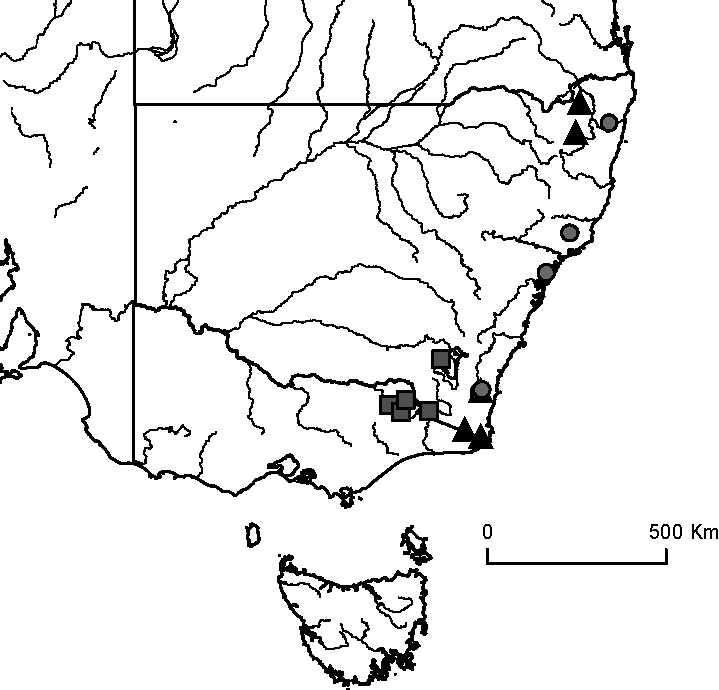
\includegraphics[width=12cm,keepaspectratio=true]{Ch2map.pdf} % figures can be in pdf, png, jpeg or eps format
\caption[Location of fifteen field study sites across south-eastern Australia.]{\small{Location of fifteen field study sites across south-eastern Australia chosen to represent the three major hydrological classes of south-east Australia. Hydrological class membership is denoted by:  $\blacksquare$ stable winter baseflow, $\blacktriangle$ unpredictable baseflow, \textbullet  unpredictable intermittent.}}
\label{fig:Ch2_F1} % label for cross-referencing
\end{center}
\end{figure}   
\clearpage

\subsection{Species abundance and trait data collection}
Data collection was undertaken between December 2012 and May 2013. At each site, a 10 m by 50 m plot was marked out, with the longest edge abutting the channel edge. Criteria for selection of plot locations were: geomorphic homogeneity (the plot comprising only sloping bank where possible) and lack of anthropogenic disturbance such as built structures, roads or tracks, recent logging or clearing (in the last 20-30 years), herbicide spraying or animal grazing. Variation in the maximum height above the channel edge between plots was kept to within approximately 1.5 m.

Proportional cover of all woody species was assessed within three strata: shrub (1-4 m), sub canopy (4-8 m) and canopy ($>$8 m). Species were identified using appropriate field guides, and were verified against herbarium specimens at the Macquarie University Herbarium. Some specimens were identified by staff at the Royal Botanic Gardens, Sydney. 

Wood samples were collected from woody species present within the plot at $>$1\% cover in shrub, sub canopy or canopy strata, and which had trunks robust enough to core. A 100 mm wood sample from each of two individuals per species was extracted using a 5.15 mm diameter, triple threaded increment borer (Hagl�f Sweden). Samples were extracted from the base of the main trunk, 10 cm above the leaf litter level, and air-dried at 20-45 \textsuperscript{o}C. On return to the laboratory, samples were rehydrated to saturation in deionised water and 10 mm sections of mature heartwood were cut flush with a razor, using visual inspection of vessel occlusion as an indicator of maturity. Sections were measured (x, y and z dimensions) to the nearest 0.01 mm with callipers (Mitutoyo America, Illinois USA) to calculate wet volume, then oven-dried at 80 \textsuperscript{o}C for 48 hours and weighed using a microbalance (Mettler Toledo, Greifensee, Switzerland). Wood density was then calculated as the ratio of oven dry mass to wet volume (g/cm\textsuperscript{3}).

Species which were present in plots but which could not be cored due to small size were assigned averaged values of wood density from the same species measured at other sites, where possible. Remaining species were assigned values from peer-reviewed literature sources. Appendix 1 contains further details about the dataset, including data density information.

\subsection{Hydrological analysis}
Daily discharge data pertaining to each field site were collated from the PINNENA CW 10.1 database (NSW Office of Water, Department of Primary Industries) and the NSW Office of Water Continuous Water Monitoring network website \url{(http://realtimedata.water.nsw.gov.au/water.stm)} for NSW sites, and the Victoria State Government�s Water Measurement Information System website \url{(http://data.water.vic.gov.au/monitoring.htm)} for Victorian sites. Where possible, 30 year time series were obtained, spanning years 1983 � 2012. Records were truncated for three sites, spanning 15, 19 and 28 years. Missing data were approximated using the Time Series Manager module in River Analysis Package \citep{marsh2003river}. Consistency of the resulting outputs were checked by visual inspection of hydrographs. For Mammy Johnson�s River, Mann River, Sportsman�s Creek and Wallagaraugh River, multiple linear regression was chosen as the most appropriate method for estimating missing data values. Linear interpolation was used for Jilliby Creek data. Daily discharge data for the remaining sites were complete.

A set of 24 hydrological metrics was pared from the full set described by \citet{Kennard2010}.  These metrics were chosen to be representative of variability in high flow magnitude and frequency as well as predictability and consistency of water availability in the riparian environment (see Table \ref{tab:Ch2_T1} for a description). We used the Time Series Analysis module in River Analysis Package to generate these metrics. Means and coefficients of variation were calculated for most metrics to indicate central tendency as well as spread within the data. Low and high spell metrics were thresholded at the 5th and 95th percentiles, respectively, with a flood independence criterion of 7 days between peak events. Twenty year average return interval (ARI) flood magnitude was also calculated with a flood independence value of 7 days between peaks. Colwell's Indices were calculated using mean flow values over monthly time periods and a class distribution of 11 flow classes. Metrics of flow magnitude which had units ML / day were normalised by mean daily flow to allow for comparison between different sizes of river. Some metrics were correlated (see Appendix 1 for correlation analysis).


\begin{landscape}
\begin{tiny}
{\tabulinesep=1.2mm
\begin{longtabu} to \linewidth {m{5.5cm}m{3.7cm}m{2.0cm}X} 
\caption[Description of hydrological variables.]{Hydrological parameters used as metrics of variability in high flow magnitude and frequency and predictability and consistency of water availability in the riparian environment. * - normalised by mean daily flow (ML/day)} \\
\label{tab:Ch2_T1} \\
\hline
% -----------------These are headings----------------------------------%
\textit{Variable} & \textit{Abbreviation} & \textit{Units} & \textit{Description} \\ 
%
\endfirsthead
%
%\multicolumn{4}{c}%
%{{\bfseries  Continued from previous page}} \\
%\hline
%
\hline
\textit{Variable} & \textit{Abbreviation} & \textit{Units} & \textit{Description} \\ \hline
\endhead
%
%\hline \multicolumn{4}{|r|}{{Continued on next page}} \\ \hline
%\endfoot
%
%\hline
%\multicolumn{4}{|r|}{{Concluded}} \\ \hline
%-----------Headings end---------------------------------
%\endlastfoot
\hline
\multicolumn{4}{l}{\textbf{Flood frequency and magnitude}} \\
Mean magnitude of high spells * & HSPeak & dimensionless & \multirow{1}{*}{\parbox{8.2cm}{High spells are periods of flow above the 95th percentile on the flow duration curve. We were interested in how frequently these conditions occurred over the time series as well as the mean magnitude of peak flows during these periods. 20 year average return interval (ARI) floods are extreme flow events that have the potential to re-work the fluvial landscape. Together, these metrics indicate the intensity and frequency of mechanical stress experienced by plants in the riparian zone.}} \\
CV of all years' mean high spell magnitude & CVAnnHSPeak & dimensionless &  \\
20 year ARI flood magnitude * & AS20YrARI & dimensionless &  \\
Mean of all years' number of high spells & MDFAnnHSNum & year\textsuperscript{-1} &  \\
CV of all years' number of high spells & CVAnnHSNum & dimensionless &  \\[0.6cm]
%\tabularnewline
\hline
\multicolumn{4}{l}{\textbf{Rise and fall rates}} \\
Mean rate of rise * & MRateRise & day\textsuperscript{-1} & \multirow{1}{*}{\parbox{8.2cm}{Rise and fall rates represent flow �flashiness�. Fast rise rates are associated with flood waves and intense mechanical stress to plant stems. Slow fall rates keep exposed substrate moist for longer periods, which may produce favourable conditions for germination. Historical discharge records are unfortunately limited to daily resolution, so are unable to fully capture flood discharge shapes. High variability between years indicates the occurrence of extreme events which may not have been captured by the mean value.}} \\
Mean rate of fall * & MRateFall & day\textsuperscript{-1} &  \\
CV of all years' mean rate of rise & CVAnnMRateRise & dimensionless &  \\
CV of all years' mean rate of fall & CVAnnMRateFall & dimensionless &  \\[1.1cm] 
%\tabularnewline
%\tabularnewline
\hline
\newpage
\multicolumn{4}{l}{\textbf{Baseflow index}} \\
Baseflow index & BFI & dimensionless & \multirow{1}{*}{\parbox{8.2cm}{Baseflow index is calculated using the ratio of flow during average conditions to total flow. It is a useful metric of consistency of water availability, in that it is maximised when average flow conditions dominate, and minimised when total flow is dominated by above average flow events. Intra-annual variability in baseflow index measures how predictable baseflow index is between years.}} \\
CV of all years' Baseflow Index & CVAnnBFI & dimensionless &  \\[1.2cm]
%& & & & \\
%\tabularnewline
\hline
\multicolumn{4}{l}{\textbf{Low flow magnitude, frequency and duration}} \\
CV of all years' mean low spell magnitude & LSPeak & dimensionless & \multirow{1}{*}{\parbox{8.2cm}{Low spells are periods of flow below the 5th percentile on the flow duration curve. We were interested in how frequently these conditions occurred over the time series as well as the mean and interannual variability in magnitude and duration of low flows.}} \\
Mean magnitude of low spells & CVAnnLSPeak & dimensionless &  \\
Mean of all years' number of low spells & MDFAnnLSNum & year\textsuperscript{-1} &  \\
CV of all years' number of low spells & CVAnnLSNum & dimensionless &  \\
Mean duration of low spells & LSMeanDur & days &  \\
CV of all years' low spell mean duration & CVAnnLSMeanDur & dimensionless &  \\
Mean flow during driest week of the year * & MA.7daysMinMean & dimensionless &  \\
Mean days per year under 0.1ML/day flow & MDFAnnUnder0.1 & days/year &  \\
CV of all years' days per year under 0.1ML/day flow & CVAnnMDFAnnUnder0.1 & dimensionless &  \\[0.3cm]
%\tabularnewline
\hline
\newpage
\multicolumn{4}{l}{\textbf{Colwell's indices}} \\
Constancy of monthly mean daily flow & C\_MDFM & dimensionless & \multirow{1}{*}{\parbox{8.2cm}{Colwell's indices provide a measure of the seasonal predictability of flow events and therefore water availability within the riparian zone. Constancy (C) measures uniformity of flow across seasons, and is maximised when flow conditions do not differ between seasons. Contingency (M) is a measure of interannual uniformity in seasonal flow patterns, and is maximized when seasonal patterns of flow are consistent between years.  We generated Colwell's indices for both average flow conditions and minimum flows conditions.}} \\
Contingency of monthly mean daily flow & M\_MDFM & dimensionless &  \\
Constancy based on monthly minimum daily flow & C\_MinM & dimensionless &  \\
Contingency based on monthly minimum daily flow & M\_MinM & dimensionless & \\[0.9cm]
%\tabularnewline
\hline
\end{longtabu}}
\end{tiny}
\end{landscape}
\clearpage

\subsection{Wood density analysis}
All statistical analyses were performed using the R statistical programming environment \citep{RCoreTeam2015}. The R code used for these analyses can be retrieved from \url{https://github.com/jamesrlawson/riparian-WD/tree/master/scripts}. Statistical significance was interpreted at alpha = 0.05. 

\subsubsection{Characterising community-level variation in wood density}
To investigate variation in wood density across hydrological gradients at the community level, community weighted means (CWM) of wood density were generated for each site. Species relative abundance was compiled from records of percent cover at the shrub (1-4 m), sub canopy (4-8 m) and canopy ($>$8 m) strata.  Wood density values were then weighted according to species relative abundance and summed to produce the CWM. This method integrates particular trait values with their real world abundance as a measure of �performance�, while providing a useful reduction in data dimensionality. Wood density varies only over one order of magnitude, while exhibiting relatively high intra-species plasticity. As such, CWMs work well for environmental gradient studies of wood density because the focus is maintained on the functional characteristics of the community, rather than on species \textit{per se}.

We also calculated community weighted variance (CWV) in wood density for each site to characterise the dispersion of wood density values within communities. CWV describes divergence from the mean trait value of a community \citep{Schleuter2010}. When trait values of abundant species are clustered towards the mean, divergence is low. Conversely, divergence is high when abundant species are distributed towards the extremes of the trait range \citep{Villeger2008}. Variance could not be calculated for Site 2 (Wallagaraugh River, unpredictable baseflow category) as only a single woody species was found at $>$ 1 \% cover at this site. This site was therefore omitted from subsequent analyses of CWV.

\subsubsection{Testing relationships between wood density and hydrological conditions}
Ordinary least-squares regression models were generated for selected metrics to determine relationships between hydrological gradients and CWMs. Linear models were used except where non-linear relationships were obvious. Wood density data was normally distributed and did not require transformation. To reduce the occurrence of Type 1 statistical error, we adjusted the resulting p values using the Benjamini - Hochberg (BH) procedure for controlling family-wise error rate (stats package) \citep{RCoreTeam2015}. Although ecological rationale supported inclusion of each subgroup of hydrological metrics, a number of these metrics were correlated. The BH procedure has been shown to control the false discovery rate for positively dependent test statistics \citep{Benjamini2001}.

We identified ecologically relevant axes of variation in hydrological conditions by running a principal components analysis (stats package), \citep{RCoreTeam2015} for hydrological metrics which had significant relationships with site mean wood density values. Having established the dominance of a single relevant axis of variation in hydrology (refer Fig. \ref{fig:Ch2_F5}), we tested the fit of a quadratic model relating extent of hydrological disturbance (as characterised by site scores from the resulting first principal component) to CWV in wood density.

Spatial autocorrelation in CWM and CWV values was assessed using Moran's I (ape package), \citep{Paradis2004}.

\section{Results}
\subsection{How does mean wood density change over hydrological gradients?}
Below we describe patterns of community weighted mean wood density in relation to the hydrological variables divided into two groups: those describing frequency and magnitude of flood disturbance, and those describing predictability of water availability in the riparian zone. Regression statistics for all models are given in Table \ref{tab:Ch2_T2}.

Community mean wood density varied by 50 \% between sites. The largest, most intense flood events throughout a river�s hydrological record were found to show a strong positive relationships with mean wood density (Fig. \ref{fig:Ch2_F2}a, \ref{fig:Ch2_F2}b. Flooding frequency had no influence on wood density. Mean flood rise rate (Fig. \ref{fig:Ch2_F2}c) as well as interannual variability in flood rise and fall rates (Fig. \ref{fig:Ch2_F2}d, \ref{fig:Ch2_F2}e) were positively related to wood density; this relationship was considerably stronger for interannual variability in flood rise rate than mean flood rise rate (R2 = 0.549 vs 0.360).

\begin{table}[ht]
\doublespacing
\tiny
\centering
\caption[Statistics for regression models.]{\small{Statistics for regression models comparing hydrological metrics with site mean wood density. P.adj denotes p values adjusted by the Benjamini-Hochberg method. Significant results are shown in bold. Models used are either quadratic or linear, as shown in Fig. \ref{fig:Ch2_F2} and Fig. \ref{fig:Ch2_F3}. For non-significant relationships, statistics shown are for linear models.}}
\label{tab:Ch2_T2}
{\tabulinesep=1.2mm
\begin{tabu}to \textwidth {XXXX}
\hline
\textit{Variable}          & \textit{P}     & \textit{P.adj} & \textit{R\textsuperscript{2}}    \\ \hline
CVAnnBFI        & 0.008 & 0.031 & 0.549 \\
CVAnnMRateRise  & 0.008 & 0.031 & 0.549 \\
C\_MinM         & 0.009 & 0.031 & 0.542 \\
C\_MDFM         & 0.012 & 0.031 & 0.522 \\
HSPeak          & 0.004 & 0.031 & 0.485 \\
AS20YrARI       & 0.005 & 0.031 & 0.467 \\
LSPeak          & 0.006 & 0.031 & 0.447 \\
CVAnnMRateFall  & 0.007 & 0.031 & 0.435 \\
BFI             & 0.012 & 0.031 & 0.397 \\
M\_MDFM         & 0.013 & 0.031 & 0.388 \\
MA.7daysMinMean & 0.017 & 0.036 & 0.368 \\
MRateRise       & 0.018 & 0.036 & 0.360 \\
MDFAnnLSNum     & 0.030 & 0.055 & 0.314 \\
MRateFall       & 0.053 & 0.091 & 0.258 \\
M\_MinM         & 0.062 & 0.100 & 0.242 \\
CVAnnHSPeak     & 0.117 & 0.175 & 0.178 \\
LSMeanDur       & 0.230 & 0.325 & 0.109 \\
CVAnnLSPeak     & 0.390 & 0.493 & 0.057 \\
CVAnnHSNum      & 0.390 & 0.493 & 0.057 \\
CVAnnLSNum      & 0.454 & 0.545 & 0.044 \\
MDFAnnUnder0.1  & 0.487 & 0.556 & 0.038 \\
MDFAnnZer       & 0.553 & 0.603 & 0.028 \\
CVAnnLSMeanDur  & 0.732 & 0.747 & 0.009 \\
MDFAnnHSNum     & 0.747 & 0.747 & 0.008 \\[0.1cm] \hline
\end{tabu}}
\end{table}

%%%% FIGURE 2
\begin{figure}[ht]
\begin{center}
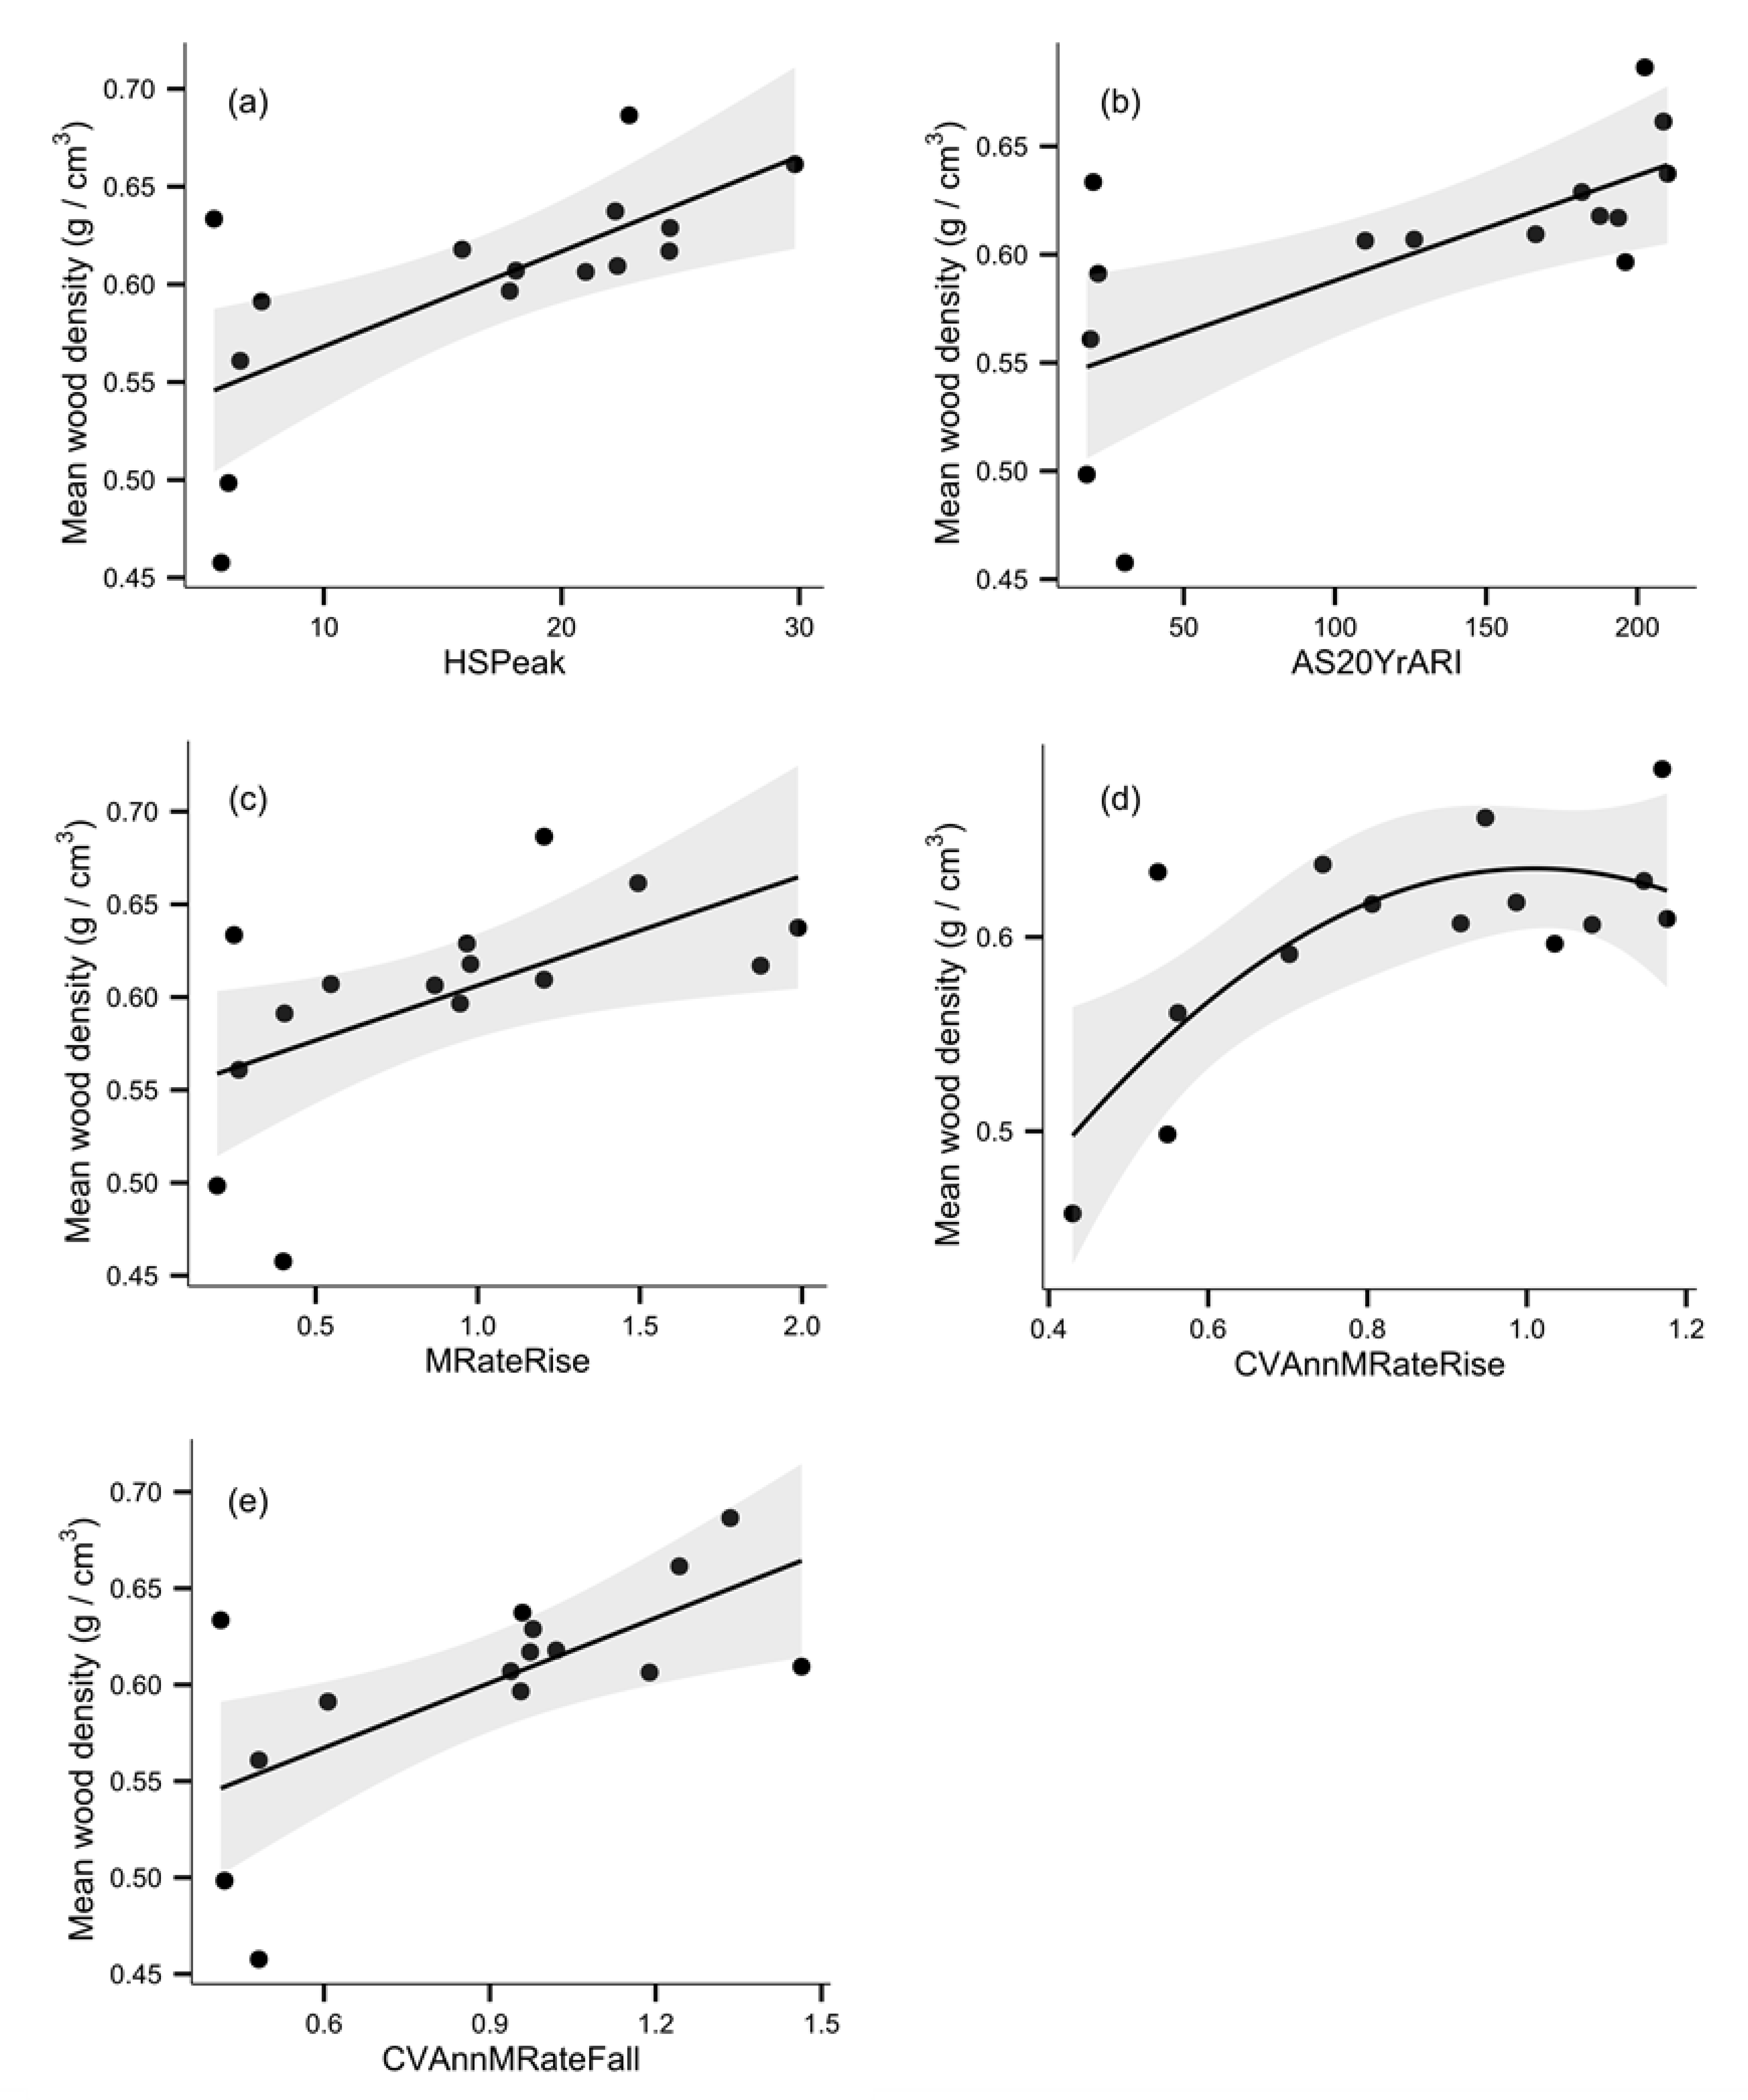
\includegraphics[width=\textwidth,keepaspectratio=true]{Ch2Fig2.png} % figures can be in pdf, png, jpeg or eps format
\caption[Relationships between wood density and flood magnitude and frequency.]{\small{Relationships between community weighted mean wood density and hydrological metrics describing a.) mean high flow magnitude (HSPeak), b.) magnitude of the 20 year average return interval flood (AS20YrARI), c.) mean rate of flow rise (MRateRise), d.) interannual variability in flood rise rates (CVAnnMRateRise), e.) interannual variability in flood fall rates (CVAnnMRateFall). Fitted lines depict ordinary least squares regression models. d. is a quadratic fit, all other models are linear fits. Shaded areas depict the smoothed 95 \% confidence interval around the regression model.}}
\label{fig:Ch2_F2} % label for cross-referencing
\end{center}
\end{figure}   
\clearpage

We found denser woody tissues were increasingly favoured as baseflow index decreased (Fig. \ref{fig:Ch2_F3}a). Wood density increased as patterns of average flow conditions became a) less uniformly distributed across seasons (Fig. \ref{fig:Ch2_F3}b), and b) less uniformly distributed year to year (Fig. \ref{fig:Ch2_F3}c). Thus mean wood density is maximised when average flow patterns are highly seasonal, but the season with which they are associated is not consistent throughout the record. A similar relationship was observed for inter-seasonal (Fig. \ref{fig:Ch2_F3}d) but not inter-annual uniformity of minimum flows. In other words, wood density was highest where minimum flows were not associated with any particular season.  Mean wood density also increased with increasing interannual variability in baseflow index (Fig. \ref{fig:Ch2_F3}e), pointing to a strong effect from years in which baseflow deviated from the mean. Wood density also decreased with mean low spell flow (Fig. 3f), and with the mean 7-day minimum flow (Fig. \ref{fig:Ch2_F3}g). For both metrics, higher values indicate wetter minimum flow conditions. Mean wood density also increased with low flow frequency (Fig. 3h). Metrics of low flow duration were not significantly associated with wood density.

No significant pattern of spatial autocorrelation was detected within values of CWM (P = 0.228). 
\begin{figure}[ht]
\begin{center}
\includegraphics[height=0.85\textheight,keepaspectratio=true]{Ch2Fig3.png} % figures can be in pdf, png, jpeg or eps format
\caption[Relationships between wood density and variability in water availability]{\small{Relationships between community weighted mean wood density and hydrological metrics describing a.) baseflow index (BFI), b.) contingency of monthly mean daily flow (M\_MDFM), c.) constancy of monthly mean daily flow (C\_MDFM), d.) constancy of monthly minimum daily flow (C\_MinM), e.) interannual variability in baseflow index (CVAnnBFI), f.) mean low flow magnitude (LSPeak), g.) mean flow during driest week of the year (MA.7days.MinMean), h.) annual frequency of low flows (MDFAnnLSNum). c. � e. are quadratic fits, all other models are linear fits. Shaded areas depict the 95 \% confidence interval around the regression model}}
\label{fig:Ch2_F3} % label for cross-referencing
\end{center}
\end{figure}   
\clearpage

\subsection{What are the principal components of variation in hydrological conditions that explain variation in wood density?}
Hydrological metrics that significantly explained site mean wood density were highly correlated in our dataset. Principal Components Analysis (PCA) identified one dominant axis within these metrics, representing 80.3 \% of variation (Fig. \ref{fig:Ch2_F4}). The remaining variation was split between several minor axes; PCA2 represented 6.3 \% of variation and the remaining axes each represented less than 3 \% of variation.

PC1 represents a gradient of environmental harshness that integrates baseflow characteristics, seasonality and flooding intensity. Metrics which are maximised under conditions of weak seasonality, high predictability and low variability of water availability were loaded towards the positive end of the PC1 axis, while metrics that are maximised under conditions of high interannual baseflow variability and high intensity flooding were loaded towards the negative end. Stable winter baseflow rivers exhibited lower site mean wood density, and were clustered at the �mild� positive end of the PC1 gradient. Unpredictable baseflow and unpredictable intermittent rivers overlapped across PC1 and were located distally towards the �harsh� negative end, and were associated with higher site mean wood density. The results of the PCA analysis illustrated that variation in wood density is largely described by a single axis of variation from low to high variability in flow.

\begin{figure}[h]
\begin{center}
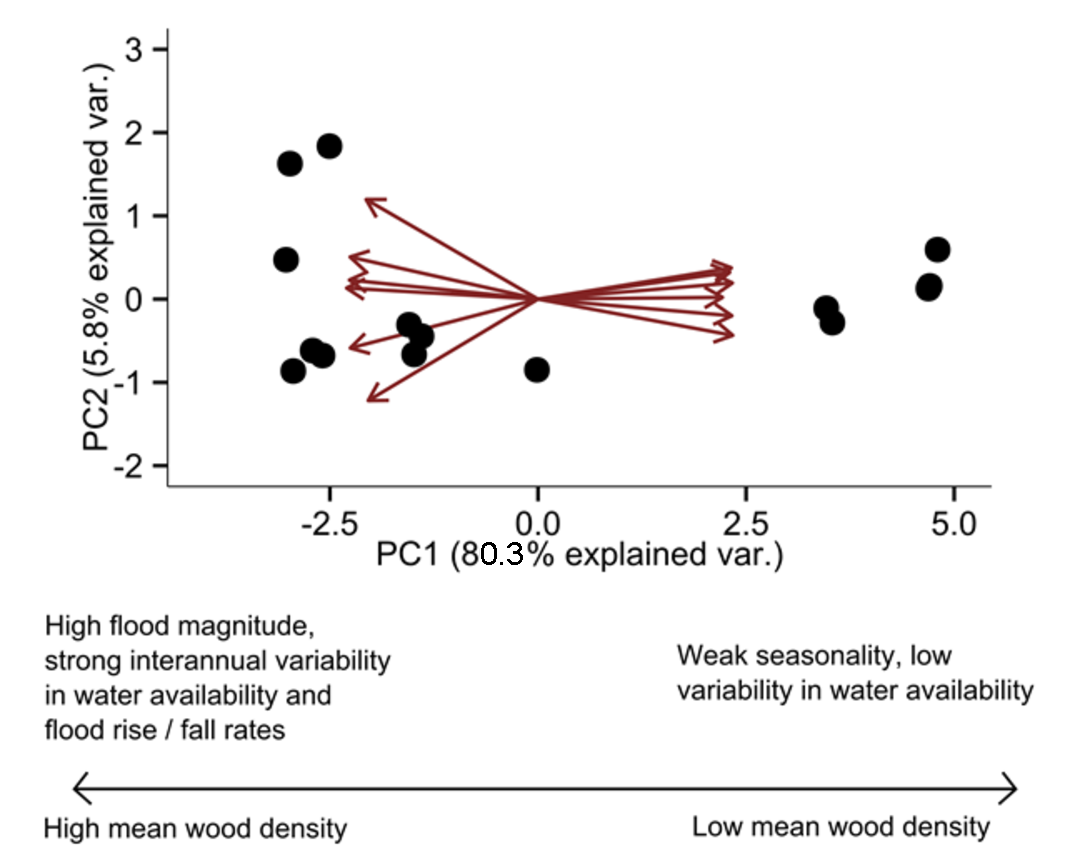
\includegraphics[width=12cm]{Ch2PCAbiplot.pdf} % figures can be in pdf, png, jpeg or eps format
\caption[PCA biplot of sites according to significant hydrological relationships with wood density.]{\small{Biplot of sites ordinated across the first two principal components as determined from Principal Components Analysis of hydrological metrics displaying significant relationships with mean wood density across 15 sites in south eastern Australia. Points represent individual sites. PC1 explains 80.3 \% of the variation in hydrology among the sites and represents a gradient of harshness of environmental conditions.}}
\label{fig:Ch2_F4} % label for cross-referencing
\end{center}
\end{figure}   

\subsection{Is there a relationship between hydrological disturbance and within-community dispersion of wood density?}
No individual metrics describing hydrological disturbance showed significant relationships with CWV following p-value adjustment. The relationship between the PC1 axis and CWV in wood density could be significantly explained by a quadratic model, however (R2 = 0.450, P = 0.037) (Fig. \ref{fig:Ch2_F5}). The fitted curve shows a peak in CWV at intermediate values of PC1, which correspond to intermediate values of hydrological disturbance and variability. No significant pattern of spatial autocorrelation was detected within values of CWV (P = 0.786).

\begin{figure}[ht]
\begin{center}
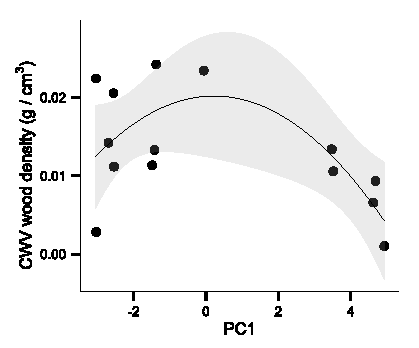
\includegraphics[width=9cm]{Ch2CWV.pdf} % figures can be in pdf, png, jpeg or eps format
\caption[Unimodal relationship between wood density CWV and PC1.]{\small{Quadratic relationship between community weighted variance in wood density and site scores for the first principal coordinate (PC1) of a Principal Components Analysis of hydrological metrics displaying significant relationships with mean wood density (see Fig. 4), (R2 = 0.450, P = 0.037). Variance peaks at intermediate values of hydrological disturbance, as described by the PC1 axis. Shaded areas depict the 95 \% confidence interval around the regression model.}}
\label{fig:Ch2_F5} % label for cross-referencing
\end{center}
\end{figure}   
\

\section{Discussion}
We sought to understand how hydrology might influence wood density, a key plant functional trait. We asked whether mean wood density could be explained by the degree of flooding disturbance or hydrological unpredictability in the riparian zone, and whether dispersion of wood density peaks in intermediately disturbed communities. To summarise, we found evidence that mean riparian wood density is positively related to flood magnitude and flow rise and fall rates, as well as to unpredictability in flow conditions over daily, seasonal and annual timescales. We also found evidence for divergence in wood density strategy at intermediate levels of disturbance.  While wood density is a complex trait that integrates trade-offs between multiple selection pressures, we believe the strong relationships between mean wood density and hydrology demonstrated here are evidence that hydrological conditions powerfully influence plant ecological strategy in the riparian environment. 

Strong relationships with measures of interannual variability point to years in which the environment was extreme as favourable towards high wood density. Several relationships were described best by quadratic models, indicating a maximum above which variation in hydrology ceases to be associated with changes in mean wood density. Predictable hydrologies and weak flooding disturbance intensity were associated with a greater range of mean wood density values. This variability may be driven by other environmental factors, which become less influential as hydrological forcing increases.  We also found that for \textit{Casuarina cunninghamiana}, a common riparian species in SE Australia, intraspecific variation in wood density responded strongly to hydrology (see Appendix 1, Fig. 1).

Specific aspects of high flow hydrology drove variation in wood density. Mean wood density was not correlated with the frequency of high flow spells, which individually may not correspond to significant disturbance events, depending on the hydrological characteristics of the given river. Rather, it was the actual magnitude of flow during high flow periods that was important. High rates of flow rise and fall, which may associated with entrainment of large debris into the flood channel and subsequent bank deposition \citep{Cadol2010}, were also associated with high community wood density. Interannual variability in rate of flow rise was a substantially stronger predictor of wood density than the mean value, suggesting a greater influence of flow rise rates in extreme years than the general mean. A pattern is apparent then, in which mean wood density in riparian communities is driven by powerful but relatively rare flow events (e.g. 10 to 20 year average return interval flood). Such floods are likely to be large enough to influence demographics, but not necessarily catastrophic (i.e. presenting no opportunity for survival). The abundance of high wood density strategies in these environments indicates that infrequent but high-stakes events may be a greater selective pressure in riparian plant communities than average conditions. For densely wooded species, persistence may be more influential on population dynamics than individual growth rates or fecundity \citep{Adler2014}. We therefore suggest that a �brick house� ecological strategy is favoured in riparian environments that experience intense flooding. This suggestion concurs with findings that trees on windy slopes tend to overcompensate for mechanical stress, with investment in defences increasing cumulatively in response to stress events \citep{telewski1995wind, Cohen1999}. This cumulative effect may be important for long-lived woody species which experience multiple high magnitude floods during their lifetimes.
 
We can extend the observation about the influence of intense �pulse� flow events on wood density: plants living in environments where flow occurs unpredictably and largely within specific events, rather than being evenly distributed throughout time, are likely to experience more intense pulses of water stress (i.e. low soil moisture). High wood density may be symptomatic of wood anatomy strategies that allow plants to tolerate water stress \citep{Hacke2001, Jacobsen2005, Jacobsen2007}. Numerous studies have discussed the role of various anatomical components of woody tissue in stabilising xylem against cavitation when plants are under severe water stress, but the exact role that woody fibres play in stabilising xylem vessels appears to be inconsistent \citep{Martinez-Cabrera2009}. Overall, resistance against cavitation emerges from complex interactions between wood anatomical traits \citep{Lens2011, Zieminska2013} and$/$or aboveground biomass production traits, both of which are tangentially related to wood density. With the exception of ephemeral dryland rivers, riparian environments tend not to be severely water limited, so specifically constructing woody tissue to deal with constant water stress may not be advantageous. For plants that are habituated to plentiful soil moisture, however, having no backup strategy for surviving drought conditions may be risky \citep{Horton2013}.

A more compelling rationale for our findings is that riparian woody plants are again overcompensating for the possibility of uncommon but intense stress events. In the absence of predictable cues about timing of watering flows, conservative resource-use phenotypes such as higher wood density would be favoured \citep{Valladares2007}. Environmental unpredictability may act as a modifier which shifts ecological strategy in favour of conservative resource use (for which wood density acts as a proxy, in this case). We can observe this effect in intraspecific variation (see Appendix 1, Fig. 1) in wood density for the rheophytic (i.e. confined to frequently flooded substrates) species \textit{C. cunninghamiana}: interannual variability in baseflow index, contingency of monthly minimum daily flow (M\_MinM) and contingency of monthly mean daily flow (M\_MDFM) describe interannual variability in water availability and all show strong relationships with intraspecific variation in \textit{C. cunninghamiana} wood density. Traits associated with conservative resource use and better recovery following periods of stress may actually confer as much or greater fitness than traits associated with coping with the stress itself \citep{Gutschick2003}.
  
Conservative resource use and heavy investment in structural strength fit within the �resister� category of riparian plant strategies described by Naiman \& Decamps' (1997) classification of riparian plant life history strategies. �Invader� strategies with which species avoid harsh hydrological conditions by achieving sexual maturity as fast as possible are also common to the riparian environment \citep{Naiman1997, Woolfrey2001}. For pioneer species employing a fast relative growth rate, low wood density ecological strategy would be benefited by repeated setbacks to early successional conditions \citep{Westoby1998}. Co-existence at intermediate disturbance intensities of a broad spectrum of strategies between �invading� and �resisting� may be responsible for the observed peak in wood density CWV, but this suggestion is difficult to substantiate using our dataset, as only a few sites were present in the middle range of the PC1 axis.
 
Under our argument, where hardy rheophytic species use high wood density ecological strategies to cope with powerful floods and unpredictable watering regimes, we would expect species such as \textit{Casuarina cunninghamiana} (Casuarinaceae) and \textit{Tristaniopsis laurina} (Myrtaceae) (two of the most common riparian species in our study region) to have the highest wood density in our dataset. However both species exhibited highly variable trait values, ranging approximately between the median value and the 75th percentile. As with \textit{C. cunninghamiana}, \textit{T. laurina} is a light-demanding coloniser of within- and near-channel landforms \citep{Webb2002}. By establishing in close proximity to the channel, seedlings of these species must balance the risks of flooding with the advantages of growth unencumbered by competition for light or space. Maintaining a high relative growth rate, at least until the trees are physically large enough to endure flooding, allows these species to quickly fill space and build photosynthetic tissue (i.e. invading) \citep{Melick1990}. If parallels with tropical rainforest species hold \citep{King2006, Kraft2008, Poorter2008, Poorter2010, Wright2010}, this strategy will not be conducive to setting down dense wood (i.e. resisting). In addition to morphological adaptations in \textit{T. laurina} such as multi-stemmedness, narrow leaves and growth streamlined against the direction of flow \citep{steenis1981rheophytes, Webb2002}, the trade-off between flood resistance and rapid resource acquisition and growth during establishment serves to explain why the optimal wood density for rheophytic species might occupy a central position along the axis of wood density. Nonetheless, the wide plasticity in wood density shown by \textit{C. cunninghamiana} and \textit{T. laurina} suggests that intraspecific variation contributes to the species� capacity to track hydrological gradients. Thus intraspecific variation in these species influences community mean wood density despite their relatively moderate species-specific mean wood density.
 
Notably, it is the tall, facultative riparian species from rainforest sites that had the highest wood density in our dataset. Lacking the morphological adaptations required to thrive directly along the channel edge, these species may rely solely on generating mechanically strong stems to withstand flooding. High wood density species tended to occur further up the bank, so would be subject to only the more intense flooding events (and least moisture availability). Since succession typically advances with elevation above the channel edge \citep{Tabacchi1998}, this observation agrees with previous work showing increasing wood density along a successional gradient \citep{Falster2005}. Further parallels in the existing wood density literature are also evident here, where high wood density individuals were much less likely to experience major wind damage following a cyclone \citep{Curran2008}.

The gradient identified by principal components analysis integrates predictability of water availability, seasonality and flood intensity into a single axis of hydrological variation. It is not possible to tease out individual drivers of variation in mean wood density, as the conditions associated with both environmental unpredictability and mechanical disturbance act in unison to drive community wood density towards higher mean values.
 
Community weighted variance in wood density showed a quadratic distribution across this gradient of �hydrological harshness�. Previous work has described a negative relationship between community-level variance in wood density and abiotic stress (using high latitude and elevation as proxies for stressful environments) \citep{Swenson2007}. Rather than constricting trait values, intermediate levels of pulsed fluvial disturbance may promote trait diversity by retarding competitive exclusion \citep{Huston1979, Naiman1997}, whilst simultaneously generating structurally heterogeneous habitat \citep{Corenblit2007}. While the fit of our model is statistically significant, the paucity of values through the middle range of the PC1 axis gives rise to error around the peak of the fitted curve; interpretation of this result therefore necessitates some caution.
 
Damming and water extraction, and changing climatic conditions are altering hydrology globally \citep{Nilsson2000, stocker2013climate}. Artificial flow modification by damming and water extraction reduces overall flow volume and the magnitude and frequency of high flow events, while increasing flow predictability, altering seasonality and limiting channel-floodplain connectivity \citep{Maheshwari1995, Graf2006}. In these altered conditions, terrestrial species with softer wood and faster growth rates may encroach on what was once the province of rheophytic assemblages adapted to flooding and less predictable hydrological conditions. The converse of this situation is presented by predictions of future climatic conditions: in Australia, warming of 0.4 - 0.7  \textsuperscript{o}C has occurred since 1950 \citep{Hennessy2007}, associated with a reduction in rainfall across southern and eastern regions of the continent \citep{Smith2004}, and an increase in intensity and frequency of droughts \citep{Hennessy2008}. Extreme rainfall events are predicted to become more prevalent, even in areas where the trend is towards mean reductions in annual or seasonal rainfall \citep{Chiew2009}. River discharge in Australia is known to be particularly sensitive to the El Nino-Southern Oscillation (ENSO)  phenomenon that is an integral driver of the continent's climate patterns \citep{Nicholls1989, Ward2010}. Projected increases in climatic variability \citep{Hennessy2008} may therefore overlay the already strong natural variability induced by ENSO to produce significant alterations to streamflow. Under such conditions, near-channel abundance of opportunistic terrestrial species (with their broad diversity of wood density strategies) may decline in favour of rheophyte-dominated assemblages whose ecological strategies are optimized to harsh hydrological conditions.  If changes in spatial extent of climate zones can be related to changes in runoff - a complicated but progressing area of research in hydroclimatology \citep{Peel2011} - functional approaches to ecohydrology can give insight into likely changes in riparian plant assemblages and associated changes in ecosystem function.

\section*{Conclusion}
Our study emphasises the importance of hydrological conditions, particularly disturbance and environmental unpredictability, as determinants of ecological strategy in riparian plant communities. These relationships may be generalisable to diverse biomes, given the strong constraints imposed by flooding and fluctuating water availability on woody plant ecological strategies in many riparian environments.  The marked influence of rare, high intensity floods on wood density is likely to have significant ecological consequences for riparian plant communities in a south-east Australian context, and potentially in other regions where increasing climatic variability and frequency of extreme events are hallmarks of climate change predictions.

\section*{Acknowledgements}
Tanja Lenz gave invaluable advice and support throughout the project. Saskia Grootemaat, Ashley Vey, Urvashi Lallu, Julia Atkinson, Sally Lawson and Anthony Manea gave their time and inspiration in the field. We also wish to thank the officers of the New South Wales Parks and Wildlife Service and Parks Victoria who provided logistical advice and support, and the landowners who were so kind as to let us work and stay on their properties. Thanks also to Alan Baldry for his help in the herbarium, and to the PIREL group at Macquarie University for their support. Finally, we would like to thank Stephen Bonser and two anonymous reviewers for their knowledge and insight.

\section*{Data availability}
Data are available through DataDryad, doi:10.5061/dryad.72h45 \citep{Lawson2015}.
\clearpage


%%%%% REFERENCES % this is in a new chapter due to the memoir format
\renewcommand\bibname{{References}} 
\begin{small}
\bibliographystyle{apalike}
\bibliography{library.bib}
\end{small}









\clearpage

%%%%%%%%%%%%%%%%%%%%%%%%%%%%%%%%
% CHAPTER 3

\chapter[Heterogeneous flows foster heterogeneous assemblages: relationships between functional diversity and hydrological heterogeneity in riparian plant communities][Functional diversity in SE Aus]{Heterogeneous flows foster heterogeneous assemblages: relationships between functional diversity and hydrological heterogeneity in riparian plant communities}
\newpage

\section*{Abstract}
Riparian ecosystems are biophysically complex and highly diverse taxonomically, structurally and functionally. While many environmental factors determine the structure and function of riparian vegetation communities, hydrology is thought to be the ‘master variable’. Flooding and variability in water availability are known to be key drivers of taxonomic diversity, but their influence on the functional trait diversity of riparian vegetation communities remains largely unexplored.

We collected data on species abundance, quantitative plant functional traits and hydrology from 15 sites distributed across south-eastern Australia to address the following questions: (a) is functional trait diversity related to frequency and magnitude of flooding disturbance? (b) is functional trait diversity related to variability in seasonal water availability within the riparian zone?

We confirm that metrics describing both flooding disturbance and patterns of water availability exhibit strong relationships with functional trait diversity in riparian vegetation communities of south-eastern Australia. Our key finding is that functional trait diversity in these systems tends to be positively associated with variability in hydrological conditions and the intensity of rare, high magnitude flooding events, rather than average patterns of flow.

Our study highlights the importance of extreme flooding events and temporal patterns of water availability as determinants of diversity in riparian vegetation communities. These relationships may have significant consequences for plant communities experiencing alterations to hydrology caused by anthropogenic flow modification and the changing climate. 

\clearpage

\section{Introduction}
Riparian ecosystems are biophysically complex and highly diverse taxonomically, structurally and functionally \citep{Naiman1993, Poff2002, Nilsson2002}. Extensive flow regulation of river systems and changing patterns of runoff under future climates are likely to produce dramatically different future flow regimes, with significant consequences for the diversity and functioning of riparian assemblages. Riverine conservation and rehabilitation efforts must therefore be informed by general understanding of the processes that generate patterns of diversity and drive ecosystem functioning in riparian ecosystems.

The prevailing paradigm in riparian ecology holds that heterogeneity in the riparian patch mosaic results from the sculpting action of hydrological processes across the biogeomorphic template \citep{Tabacchi1996, Palmer1997, Corenblit2007, Bornette2008}. In riparian environments, it is this intrinsic environmental heterogeneity that fosters structural, taxonomic and functional heterogeneity within vegetation communities \citep{Naiman1993, Corenblit2007, Bornette2008}. Local hydrology (river flow regime) is widely considered to be the most important determinant of community composition and functioning in riparian plant assemblages, as it dictates patterns of disturbance by flooding, as well as soil moisture availability \citep{Poff1997, Arthington2010}.

Flooding may retard competitive exclusion by resetting the patch structure of parts of the landscape and thereby enhance diversity \citep{Huston1979, Naiman1993}, or constrain assemblages to species that have ecological strategies adapted to flooding, thereby decreasing diversity \citep{Diaz1998}. General support has been found for the intermediate disturbance hypothesis \citep{connell1978diversity} with respect to the relationship between flooding intensity and taxonomic diversity (e.g. \citet{Bendix1997}, \citet{Bendix2000}, \citet{Lite2005}, \citet{Corenblit2007}. This support is not equivocal however \citep{Nilsson1989, Baker1990} and at within-reach scales the geomorphic template is also a strong control on diversity \citep{Bendix1997, ODonnell2014}.
 
In regions where riparian plants experience periodic water stress, soil moisture availability may be driven largely by hydrology \citep{Castelli2000, Nilsson2002}. Seasonal and interannual variability in patterns of disturbance and water availability are also known to influence species richness \citep{Greet2011, Catford2012, Catford2014} and this effect may be exacerbated for summer flows in hot or dry regions \citep{Garssen2014}. A study investigating drivers of riparian vegetation community structure and composition in subtropical eastern Australia identified variability in dry season flows as the hydrological variable that was most strongly associated with variation in species richness \citep{Arthington2012}.
 
Conservation and restoration activities increasingly aim to preserve the ecosystem functions associated with biological communities \citep{Aerts2011, Cadotte2011, Montoya2012}. Quantitative functional traits (such as specific leaf area, wood density, seed mass, etc.) can form the basis for mechanistic assessments of diversity that describe the range and distribution of ecological strategies in a community and their associated environmental effects. Such metrics of functional trait diversity (hereafter referred to as ‘functional diversity’) are substantially more powerful than taxonomic metrics as indicators of ecosystem functioning, ecosystem resilience and capacity to provide ecosystem services \citep{Tilman1997, Diaz1998, Hooper2005}. Reduced abundance of functionally unique species may gradually undermine ecosystem resilience or functioning, and assessment of functional diversity can be useful to diagnose degradation before species loss occurs \citep{Mouillot2013}. Assessments of ecosystem service production have also begun to give functional diversity priority over taxonomic metrics \citep{Diaz2007}.
 
Numerous metrics of functional diversity have been described in the literature \citep{Schleuter2010, Mouillot2013}. These aim to quantify 'the distribution of species and their abundances in the functional space of a given community' \citep{Mouillot2013} and typically process multidimensional trait data to output a single value describing various properties of these data. The framework described by \citet{Villeger2008}, consisting of functional richness (the volume of the convex hull circumscribing the range of trait values), functional divergence (divergence in the distribution of abundance within trait space) and functional evenness (the evenness of this distribution in trait space), has been commonly used to describe functional diversity (e.g. \citet{Biswas2010}, \citet{Pakeman2011}, \citet{Savage2012}, \citet{Clark2012}). Functional dispersion (FDis), defined as the abundance-weighted mean distance in multivariate trait space of individual species to the centroid of all species in the community, represents an improvement on this framework \citep{Laliberte2010}. FDis allows for consideration of species’ abundances while integrating functional richness and functional divergence and is formulated to be independent of species richness, alleviating concerns that it merely tracks patterns of species richness (as is possible with functional richness). FDis is also known to be more robust to bias due to missing trait data than metrics such as functional richness, evenness or divergence \citep{Pakeman2014}. In an empirical assessment of specific functional diversity metrics as indicators of ecosystem functioning in a Minnesota grassland, FDis was a useful predictor of three measures encompassing above and belowground biomass production and light capture, and compared favourably with other metrics \citep{Clark2012}.

Considerably less is known about drivers of functional diversity than of taxonomic diversity in riparian plant communities. \citet{Catford2011} analysed univariate functional trait distributions to show how flow impoundment along a large river system in south-eastern Australia was associated with greater cover of exotic species and reduced functional diversity in riparian wetlands. Support for the intermediate disturbance hypothesis with respect to functional diversity has been described in communities along a gradient of disturbance associated with management for logging \citep{Biswas2010}. Similarly in agricultural systems, land-use intensification has been linked with lower functional diversity across an international dataset \citep{Laliberte2010} and the authors associated this effect with a reduced ability of communities to respond to disturbance. On the west coast of Scotland, increasing anthropogenic disturbance in arable fields, grazed grasslands, moorlands and woodlands was associated with reduced functional richness and increased functional evenness \citep{Pakeman2011}. A trend is apparent from these studies where functional diversity is inversely associated with human-induced environmental homogenisation.
 
Environmental heterogeneity is increasingly regarded as a key factor governing species richness gradients \citep{Stein2014}. To date, however, advances in quantitative ecology based on functional traits have been sparsely applied to riparian systems. Describing the influence of hydrological heterogeneity on quantitatively derived measures of riparian functional diversity would represent a significant advance for riparian ecology and ecosystem-oriented riparian conservation.

We hypothesised that the environmental heterogeneity induced by repeated floods and fluctuating soil moisture levels should be reflected in the functional diversity of plant communities adapted to the riparian environment. We investigated the relationship between hydrologically driven environmental heterogeneity and functional diversity in riparian plant communities, using south-eastern Australia as a case study where a broad spectrum of hydrological heterogeneity is present within a relatively compact, contiguous landscape \citep{finlayson1988australia, Peel2004}.  Specifically, we asked the following questions: (1) Is functional trait diversity related to the frequency and magnitude of flooding disturbance? (2) Is functional trait diversity related to variability in seasonal water availability in the riparian zone?

\section{Methods}
\subsection{Study sites}
Fifteen riparian sites were selected along gauged, partly confined rivers in the South-East Coast and south-eastern Murray Darling drainage basins of Australia. These sites were distributed across clear gradients of ecologically relevant dimensions of hydrological variation: specifically, the magnitude, frequency, duration, timing and rates of change of flow events and patterns. The study area spanned latitude -29.467 to -37.371\textsuperscript {o}S and longitude 147.413 to 152.217 \textsuperscript{o}E. Sites spanned an altitudinal range of 23 - 732 m above sea level. Site-specific details can be found in Appendix 2a. Criteria for selection of plot locations were: geomorphic homogeneity (the plot comprising only sloping bank where possible) and lack of anthropogenic disturbance such as built structures, roads or tracks, recent logging or clearing (in the last 20-30 years), herbicide spraying or animal grazing. Variation in the maximum height above the channel edge between plots was kept to within approximately 1.5 m. Full description of site selection criteria and vegetation survey methods can be found in \citep{Lawson2015}, as this study was undertaken simultaneously and at the same sites. 

\subsection{Rationale for trait selection}
Data for the following traits were collected: specific leaf area, maximum canopy height, seed mass, wood density, flowering period length and leaf narrowness. These traits were chosen to encapsulate the key axes of variation and trade-offs relevant to ecological strategies employed by riparian plants (see Table \ref{tab:Ch3_T1} for justification and further description of functional traits).

\begin{landscape}
\begin{table}[ht]
\doublespacing
\tiny
\centering
\caption[Traits included in functional diversity analysis.]{\small{Justification for inclusion of traits in the functional diversity analysis.}} \\
\label{tab:Ch3_T1} \\
{\tabulinesep=1.2mm
%\begin{tabu} to \linewidth {m{3.2cm}m{5cm}X}
\begin{tabu} to \linewidth {lp{5cm}X}

\hline
\textit{Trait} & \textit{Definition} & \textit{Ecological strategies and trade-offs captured by trait} \\ \hline
Specific leaf area & Ratio of one-sided leaf area to oven dry mass (cm2 g\textsuperscript{-1}). & Indicates species position along the leaf economics spectrum \citep{Wright2004}. \newline Associated with trade-off between rapid leaf construction and ability to tolerate stress \citep{Reich2003}. \\
Maximum canopy height & Height above ground of apical meristem (m). & Integrates trade-off between competition for light and cost of construction and maintenance of support structures (Falster 2006). \\
Seed mass & Combined mass of the seed coat, endosperm and embryo (g). Does not include dispersal structures. & Indicates maternal investment in individual offspring \citep{Leishman2000}. \newline Influences hydrochory (via seed buoyancy) \citep{Carthey2015}, and ability to establish in different soil moisture conditions \citep{Leishman2000}. \\
Wood density & Oven dry mass divided by green volume (g cm\textsuperscript{-3}) & Confers mechanical strength to stems but costly to construct. \newline Associated with slower relative growth rates \citep{Chave2009} but greater ability to tolerate water stress and disturbance \citep{telewski1995wind, Preston2006, Lawson2015}. \\
Flowering period length & Proportion of the year spent in flower (proportion, dimensionless) & Indicates species ability to respond reproductively to favourable conditions. \\
Leaf narrowness & Ratio of average leaf width to average length (ratio, dimensionless) & Narrow leaves present less photosynthetically active tissue but can regulate temperature more efficiently and thus maintain photosynthesis in hot, dry or highly insolated (i.e. disturbed) conditions \citep{Cornelissen2003}. \newline Strongly indicative of rheophyty, the trait syndrome shared by plants adapted to growing near swift flowing, frequently flooded streams \citep{steenis1981rheophytes}. \\ \\
\hline
\end{tabu}}
\end{table}
\clearpage
\end{landscape}

\subsection{Trait dataset assembly}
The dataset for this study was assembled using measurements recorded in the field (specific leaf area, wood density), supplemented by data from published literature, private and public trait databases and Australian flora texts.. In the case that multiple values were found in the literature or online for a trait, values were excluded if they were measured from sites that were substantially different environmentally to the field site in which they were found in this study.  Remaining values were averaged. Single values for each trait were recorded, under the assumption that for our chosen traits, interspecific variation is strong enough to allow differentiation between species despite noise due to intraspecific variation, and that species trait hierarchies are largely conserved across different spatial scales and datasets \citep{Cordlandwehr2013, Kazakou2014}. Leaf narrowness was not included for grasses, while seed mass and flowering period length were not included for ferns.

Specific leaf area was measured once for each species according to the procedure defined by Cornelissen (2003). A minimum of five new but fully mature leaves from well-lit areas were taken from each of five non-contiguous individual plants. Leaves were pressed in the field to maintain fresh area and allowed to air dry at 20-45°C, then scanned and leaf area measurements made using image analysis software (ImageJ 1.48 for Windows).  Leaves were then oven dried at 70°C for 72 hours and weighed using a microbalance (Mettler Toledo, Greifensee, Switzerland). Specific leaf area was calculated as one-sided fresh area divided by oven dry mass.

Wood density data were collected according to the procedure outlined in \citet{Lawson2015}. Site-specific values were available for wood density but for the purposes of this study an overall mean value was calculated for species that occurred at multiple sites. Wood density values for species for which data was not available from the field were obtained from the Global Wood Density Database \citep{Chave2009}.

\subsection{Hydrological analysis}
Daily discharge data for each site were obtained from the PINNNENA CW 10.1 database (New South Wales Office of Water, Department of Primary Industries) and the New South Wales Office of Water Continuous Water Monitoring network website \url{http://realtimedata.water.nsw.gov.au/water.stm} for New South Wales sites, and the Victoria State Government’s Water Measurement Information System website \url{http://data.water.vic.gov.au/monitoring.htm} for Victorian sites.  Thirty year time series spanning 1983 – 2012 were obtained where possible, although three sites had truncated records of 15, 19 and 28 years. Missing data were approximated by multiple linear regression  and linear interpolation using the Time Series Manager module in the River Analysis Package \citep{marsh2003river}. Consistency of the resulting outputs were checked by visual
inspection of hydrographs. For Mammy Johnsons River, Mann River, Sportsmans Creek and Wallagaraugh River, multiple linear regression was chosen as the most
appropriate method for estimating missing data values. Linear interpolation was used for Jilliby Creek data.  We used the Time Series Analysis module in the River Analysis Package to generate a set of 23 hydrological metrics for each site, based on a reduction of the minimally redundant set of ecologically relevant metrics for Australian rivers described by \citet{Kennard2010}. These metrics were chosen as descriptors of the frequency and magnitude of flooding disturbance, as well as variability in water availability across seasons and between years (see Table \ref{tab:Ch3_T2} for descriptions and rationale for inclusion of individual metrics). Collinearity between these metrics was analysed using principal components analysis (PCA); the results of this PCA as well as summary statistics for hydrological metrics are given in Appendix 2a. Parameters used to generate hydrological metrics were identical to \citet{Lawson2015}. Metrics of flow magnitude, which had units mL day\textsuperscript{-1} were standardised by mean daily flow to allow for comparison between different river channel sizes. These metrics therefore represent ratios of flow magnitude to mean daily flow.

\begin{landscape}
\begin{tiny}
{\tabulinesep=1.2mm
\begin{longtabu} to \linewidth {m{6.5cm}m{2.5cm}m{2.2cm}X}
%\begin{longtabu} to \linewidth {lm{2.5cm}m{2.5cm}X}
\caption[Description of hydrological variables.]{Hydrological parameters used as metrics of variability in high flow magnitude and frequency and predictability and consistency of water availability in the riparian environment. * - normalised by mean daily flow (ML/day)} \\
\label{tab:Ch3_T2} \\
\hline
% -----------------These are headings----------------------------------%
\textit{Parameter} & \textit{Abbreviation} & \textit{Units} & \textit{Description} \\%
\endfirsthead
%
%\multicolumn{4}{c}%
%{{\bfseries  Continued from previous page}} \\
%\hline
%
\hline
\textit{Parameter} & \textit{Abbreviation} & \textit{Units} & \textit{Description} \\ \hline
\endhead
%
%\hline \multicolumn{4}{|r|}{{Continued on next page}} \\ \hline
%\endfoot
%
%\hline
%\multicolumn{4}{|r|}{{Concluded}} \\ \hline
%\endlastfoot
%-----------Headings end---------------------------------
\hline
\multicolumn{4}{l}{\textbf{Flood frequency and magnitude}} \\
Mean magnitude of high spells * & HSPeak & dimensionless & \multirow{1}{*}{\parbox{8.2cm}{Together, these metrics characterise patterns of flooding intensity and frequency. High spells are periods of flow above the 95th percentile on the flow duration curve. HSPeak describes the mean magnitude of peak flows during high spells throughout the record. MDFAnnHSNum describes the mean annual frequency of high spell periods. The coefficients of variation of these metrics between years characterise hydrological variability as it pertains to patterns of high flows. 20 year average return interval (ARI) floods are larger flow events with the potential to be geomorphically effective and rework the fluvial landscape.}} \\
CV of all years’ mean high spell magnitude & CVAnnHSPeak & dimensionless &  \\
20 year ARI flood magnitude * & AS20YrARI & dimensionless &  \\
Mean of all years’ number of high spells & MDFAnnHSNum & year\textsuperscript{-1} &  \\
CV of all years’ number of high spells & CVAnnHSNum & dimensionless &  \\[1.1cm] 
\hline
\multicolumn{4}{l}{\textbf{Rise and fall rates}} \\
Mean rate of rise * & MRateRise & day\textsuperscript{-1} & \multirow{1}{*}{\parbox{8.2cm}{Flow rise and fall rates describe the shape of high flow curves. Interannual variability within these metrics captures the diversity of peak flow shapes within a system. Unfortunately, these metrics are constrained to daily resolution by the limitations of historical discharge records.}} \\
Mean rate of fall * & MRateFall & day\textsuperscript{-1} &  \\
CV of all years’ mean rate of rise & CVAnnMRateRise & dimensionless &  \\
CV of all years’ mean rate of fall & CVAnnMRateFall & dimensionless &  \\[0.2cm]
\hline
\newpage
\multicolumn{4}{l}{\textbf{Colwell's indices}} \\
Constancy of monthly mean daily flow & C\_MDFM & dimensionless & \multirow{1}{*}{\parbox{8.2cm}{Colwell's indices provide a measure of the seasonal predictability of flow events and therefore water availability within the riparian zone. Constancy (C)  measures uniformity of flow across seasons, and is maximised when flow conditions do not differ between seasons. Contingency (M) is a measure of interannual uniformity in seasonal flow patterns, and is maximized when seasonal patterns of flow are consistent between years.  We generated Colwell's indices for both average flow conditions and minimum flows conditions.}} \\
Contingency of monthly mean daily flow & M\_MDFM & dimensionless &  \\
Constancy based on monthly minimum daily flow & C\_MinM & dimensionless &  \\
Contingency based on monthly minimum daily flow & M\_MinM & dimensionless &  \\[1.1cm]
\hline
\multicolumn{4}{l}{\textbf{Flow seasonality}} \\
Average mean daily flow for Spring * & MDFMDFSpring & dimensionless & \multirow{1}{*}{\parbox{8.2cm}{These metrics describe the average magnitude and variability within mean daily flows for each season. Averages and coefficients of variation are calculated across yearly means. Seasonal average mean daily flows were standardised by overall mean daily flow, so actually represent the ratio of mean daily flow in a given season to the total mean daily flow.}} \\
Average mean daily flow for Summer * & MDFMDFSummer & dimensionless &  \\
Average mean daily flow for Autumn * & MDFMDFAutumn & dimensionless &  \\
Average mean daily flow for Winter * & MDFMDFWinter & dimensionless &  \\
CV of mean daily flow for Spring & CVMDFSpring & dimensionless &  \\
CV of mean daily flow for Summer & CVMDFSummer & dimensionless &  \\
CV of mean daily flow for Autumn & CVMDFAutumn & dimensionless &  \\
CV of mean daily flow for Winter & CVMDFWinter & dimensionless & \\[0.2cm]
\hline
\end{longtabu}}
\clearpage
\end{landscape}

\subsection{Functional trait diversity analysis}
Functional dispersion characterises the distribution of species traits at a site in multivariate trait space. We used the dbFD function from the FD package for R \citep{Laliberte2010} to calculate abundance-weighted functional dispersion (FDis) from species trait values and relative abundances for each site. This package implements the method for distance-based tests for homogeneity of multivariate dispersions described by Anderson \citep{Anderson2006}.  dbFD uses Gower's method \citep{Gower1971} to generate the trait dissimilarity matrix, which can account for missing values, and automatically standardises traits by their ranges; Cailliez’s correction was applied to the matrix \citep{Cailliez1983}. Simpson’s diversity was calculated using the SYNCSA package \citep{debastiani2012syncsa}. 

Due to data limitations, only species present at $>$1 \% cover in plots were included in the analysis (n = 126, from a total of 327 species). Data deficient species lacking values for more than four traits could not be included in the analysis as they produced gaps in the distance matrix used to calculate functional diversity. Thus a final total of 107 species were included in the analysis. Data density exceeded 90 \% for all sites and averaged 97 \%; full data density information including trait specific values are shown in the Appendix 2b. All trait values were transformed by log10 prior to analysis. Summary statistics for the trait dataset are also available in Appendix 2b.
Following citept{Leps2006}, we performed principal components analysis (PCA) (stats package), \citep{RCoreTeam2015} on trait data to check for redundancy. Although not completely orthogonal, traits were well distributed across multiple principal components. Therefore we believe there is both ecological (as previously discussed) and statistical rationale to retain all six traits in the analysis.

All statistical analyses were performed using the R statistical programming environment \citep{RCoreTeam2015}. Statistical significance was interpreted at alpha = 0.05.

\subsection{Relationships between FDis, hydrological metrics and taxonomic diversity}
Ordinary least-squares (OLS) regression models were generated for the selected metrics to determine relationships between hydrological gradients and FDis. To reduce the occurrence of Type 1 statistical error, we adjusted the resulting p values using the two-step Benjamini - Hochberg (BH) procedure \citep{Benjamini2006} for controlling the false discovery rate (mt.rawp2adjp function in multtest package for R) \citep{pollard2008multtest}.
 
The utility of functional diversity metrics depends on their ability to provide non-redundant information compared with measures of taxonomic diversity. We further tested relationships (using OLS regression) between FDis and species richness and Simpson’s diversity (for species used in the analysis, present at $>$1 \% cover), and species richness for the full set of 327 species identified in the study. 

We selected a minimal multiple regression model designed to incorporate descriptors of disturbance frequency and magnitude and variability in seasonal flow. The full set of hydrological metrics was initially screened to remove metrics that were individually determined to have non-significant relationships with FDis. PCA over the remaining metrics identified one major and two minor axes of variation (PC1 – 71.4 \%, PC2 – 9.0 \% and PC3 - 8.3 \% of variance explained). For PC1 there was no clear differentiation in eigenvalues; the metric with highest individual R\textsuperscript{2} value (interannual variability in high flows) was selected. PC2 identified mean daily flow in summer and PC3 identified interannual variability in flood frequency as further sources of variability. Models were then built pertaining to all possible permutations of summation and interaction for these three metrics. Values for each metric were centred by subtracting the mean value (after \citet{Robinson2009}). Multicollinearity was tested for according to the variance inflation factor (VIF) score (HH package), \citep{heiberger2004statistical} and models were compared according to the second order of Akaike’s Information Criterion (AIC) (MuMIn package) for R \citep{barton2012mumin, burnham2002model}.

\subsection{Assessing the influence of other environmental variables}
Climatic and edaphic conditions are known to be important abiotic drivers of plant diversity at landscape scales \citep{Laliberte2013, Vazquez-Rivera2015}, and may exhibit strong interdependence with flow regime. We used a variance partitioning approach to assess the individual contributions of hydrology, climatic and edaphic conditions to modelling variation in FDis. Climate data was taken from eMast/TERN at a resolution of 0.01 degrees \citep{Hutchinson2014}.  Bioclimatic variables representing annual trends, seasonality and extremes were then calculated following the BIOCLIM concept \citep{busby1991bioclim}. Edaphic data were obtained from the CSIRO Soil and Landscape Grid of Australia at a resolution of 3 arc seconds ({\raise.17ex\hbox{$\scriptstyle\mathtt{\sim}$}} 3 m) \citep{Rossel2014, Rossel2014a, Rossel2014b, Rossel2014c, Rossel2014d, Rossel2014e, Rossel2014f, Rossel2014g, Rossel2014h, Rossel2014i, Rossel2014j; Wilford2014}. Further details on these climate and edaphic datasets are given in Appendix 2a. Optimal models explaining variation in FDis according to climatic and edaphic variables were then generated using the same process as for hydrological metrics. Variance explained by these models was partitioned by partial regression following \citet{Legendre2007}, using the function varpart in R (vegan package), \citep{Oksanen2013}. Adjusted R\textsuperscript{2}, which controls for sample size and number of predictors \citep{Peres-Neto2006}, was used to estimate the proportion of variation jointly and independently explained by each model.

\section{Results}
Below we describe patterns of variation in functional dispersion (FDis) as they relate to the hydrological metrics described in Table \ref{tab:Ch3_T2}. All models are linear apart from M\_MinM and CVMDFSummer, for which a quadratic model (df = 2,12) provided a substantially better fit. Statistics for all univariate regression models are presented in Appendix 2c.

\subsection{Is functional diversity related to the frequency and magnitude of flooding disturbance?}
Functional dispersion was positively associated with metrics describing intense but rare episodes of flooding disturbance. FDis was significantly associated with the magnitude of the 20-year average return interval flood (AS20YrARI, Fig. \ref{fig:Ch3_F1}a, adjusted p = 0.0278, R\textsuperscript{2} = 0.377). FDis was also significantly associated with interannual variability in high flow magnitude (CVAnnHSPeak, Fig. \ref{fig:Ch3_F1}b, adjusted p = 0.0152, R\textsuperscript{2} = 0.577) and rates of flow rise (CVAnnMRateRise, Fig. \ref{fig:Ch3_F1}c, adjusted p = 0.0278, R\textsuperscript{2} = 0.403) and fall (CVAnnMRateFall, Fig. \ref{fig:Ch3_F1}d, adjusted p = 0.0278, R\textsuperscript{2} = 0.390), whereas relationships with metrics describing average conditions were not significant (mean high flow magnitude, HSPeak, adjusted p = 0.065; mean flood rise rate, MRateRise, adjusted p = 0.156; mean flood fall rate, MRateFall, adjusted p = 0.157). Likewise, while interannual variability in flood frequency (CVAnnHSNum, Fig. \ref{fig:Ch3_F1}e, adjusted p = 0.0360 R\textsuperscript{2} = 0.296) was significantly associated with FDis, mean annual flood frequency was not (MDFAnnHSNum, adjusted p = 0.727). These results indicate that functional diversity is higher at sites that experience extreme flooding events and heterogeneous patterns of flow.

%%%% FIGURE 1
\begin{figure}[ht]
\begin{center}
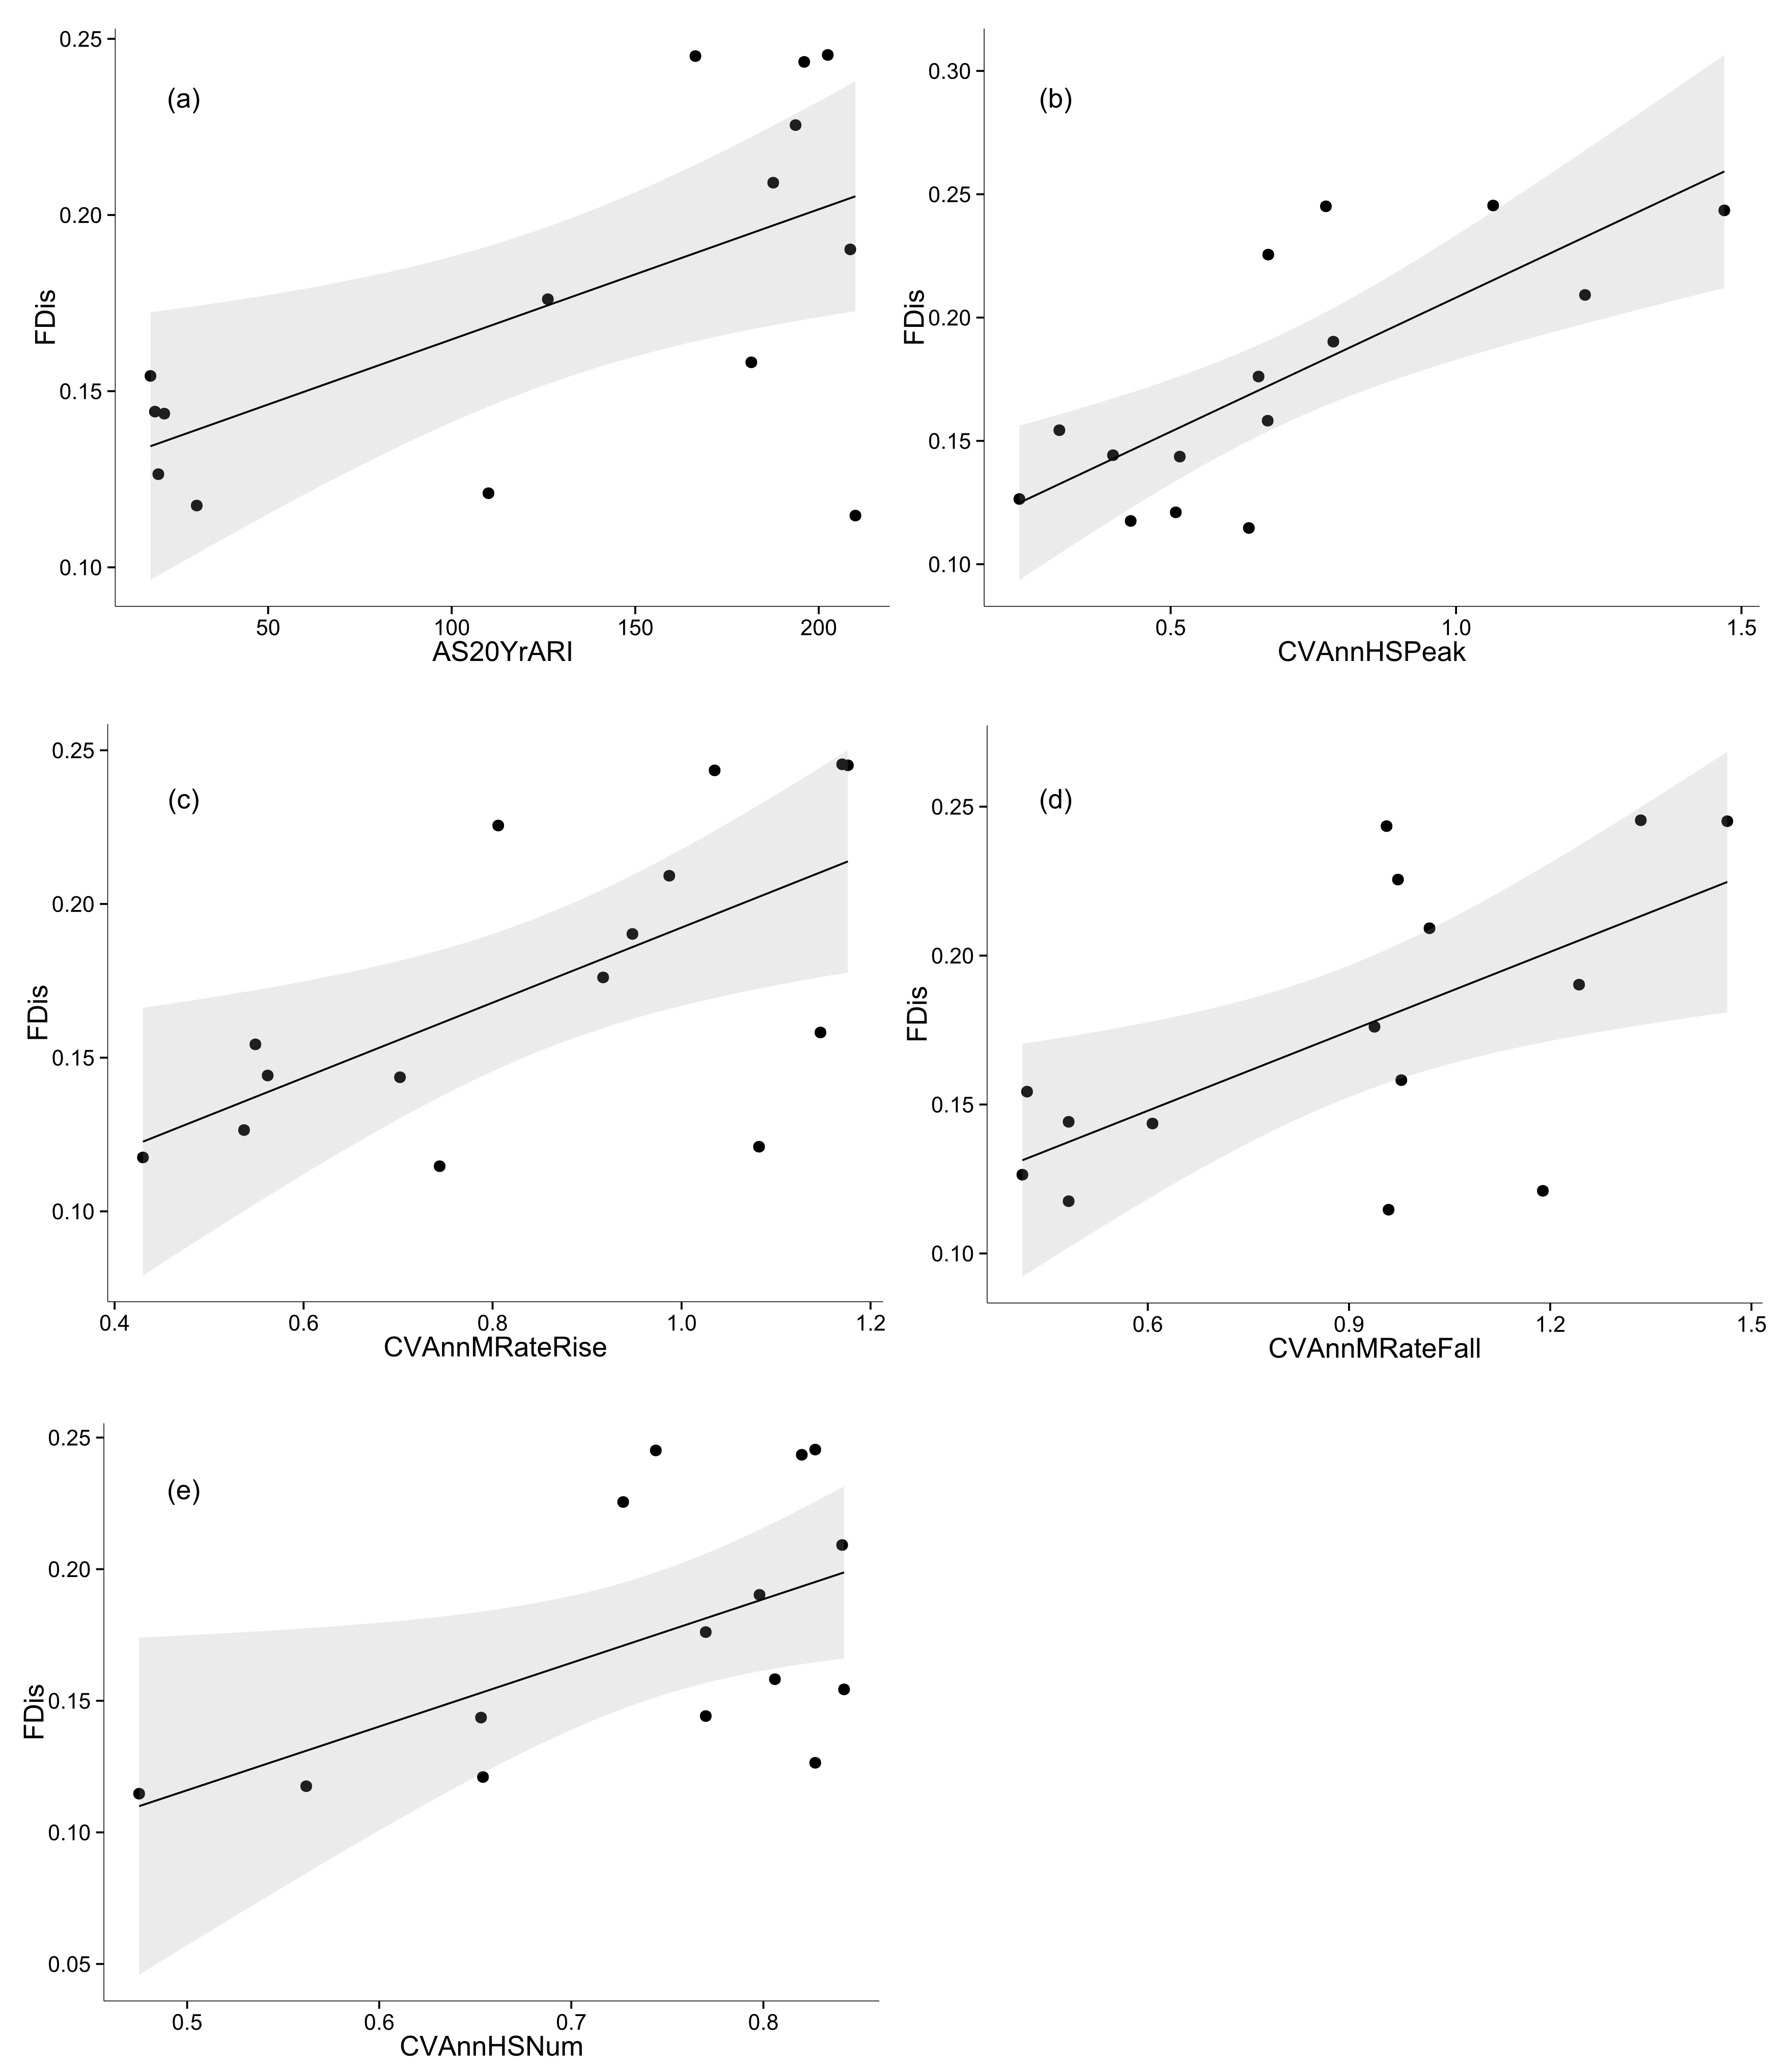
\includegraphics[width=\textwidth,keepaspectratio=true]{Ch3fig1.png} % figures can be in pdf, png, jpeg or eps format
\caption[Relationships between FDis and hydrological metrics describing flood magnitude.]{\small{Relationships between FDis and hydrological metrics describing (a) magnitude of the 20 year average return interval flood (AS20YrARI), (b) interannual variability in high flow magnitude (CVAnnHSPeak), (c) interannual variability in flood rise rate (CVAnnMRateRise), (d) interannual variability in flood fall rate (CVAnnMRateFall), (e) interannual variability in high flow frequency. Fitted lines depict ordinary least squares regression models. All models are linear fits. Shaded areas depict the smoothed 95 \% confidence interval around the regression model. All relationships shown are significant.  Units shown in Table \ref{tab:Ch3_T2}.}}
\label{fig:Ch3_F1} % label for cross-referencing
\end{center}
\end{figure}   
\clearpage

\subsection{Is functional diversity related to variability in seasonal water availability in the riparian zone?}
Functional dispersion was positively associated with variability in flow seasonality. FDis was increased when seasonal patterns of minimum (M\_MinM, Fig. \ref{fig:Ch3_F2}
a, adjusted p = 0.0278, R\textsuperscript{2} = 0.540), maximum (M\_MaxM, Fig. \ref{fig:Ch3_F2}b, adjusted p = 0.0325, R\textsuperscript{2} = 0.328) and average (M\_MDFM, Fig. \ref{fig:Ch3_F2}c, adjusted p = 0.0325, R\textsuperscript{2} = 0.347) flows became less uniform (smaller values of M) between years. In other words, at high FDis the season with which these flows were associated was not consistent through the record. FDis was not significantly explained by inter-seasonal uniformity of minimum (Fig. \ref{fig:Ch3_F2}d, C\_MinM, adjusted p = 0.1021, R\textsuperscript{2} = 0.166) or average (Fig. \ref{fig:Ch3_F2}e, C\_MDFM, adjusted p = 0.0861, R\textsuperscript{2} = 0.186) flows, although visual inspection of the scatterplots for these relationships indicates two sites at the lower bound of the x axis (i.e. strongly seasonal patterns of flow), with substantially lower FDis than predicted by the regression model. If we consider these trends, we can infer that functional dispersion was increased when discharge patterns differed strongly between seasons, but the season with which those patterns were associated was not consistent between years.

\begin{figure}[ht]
\begin{center}
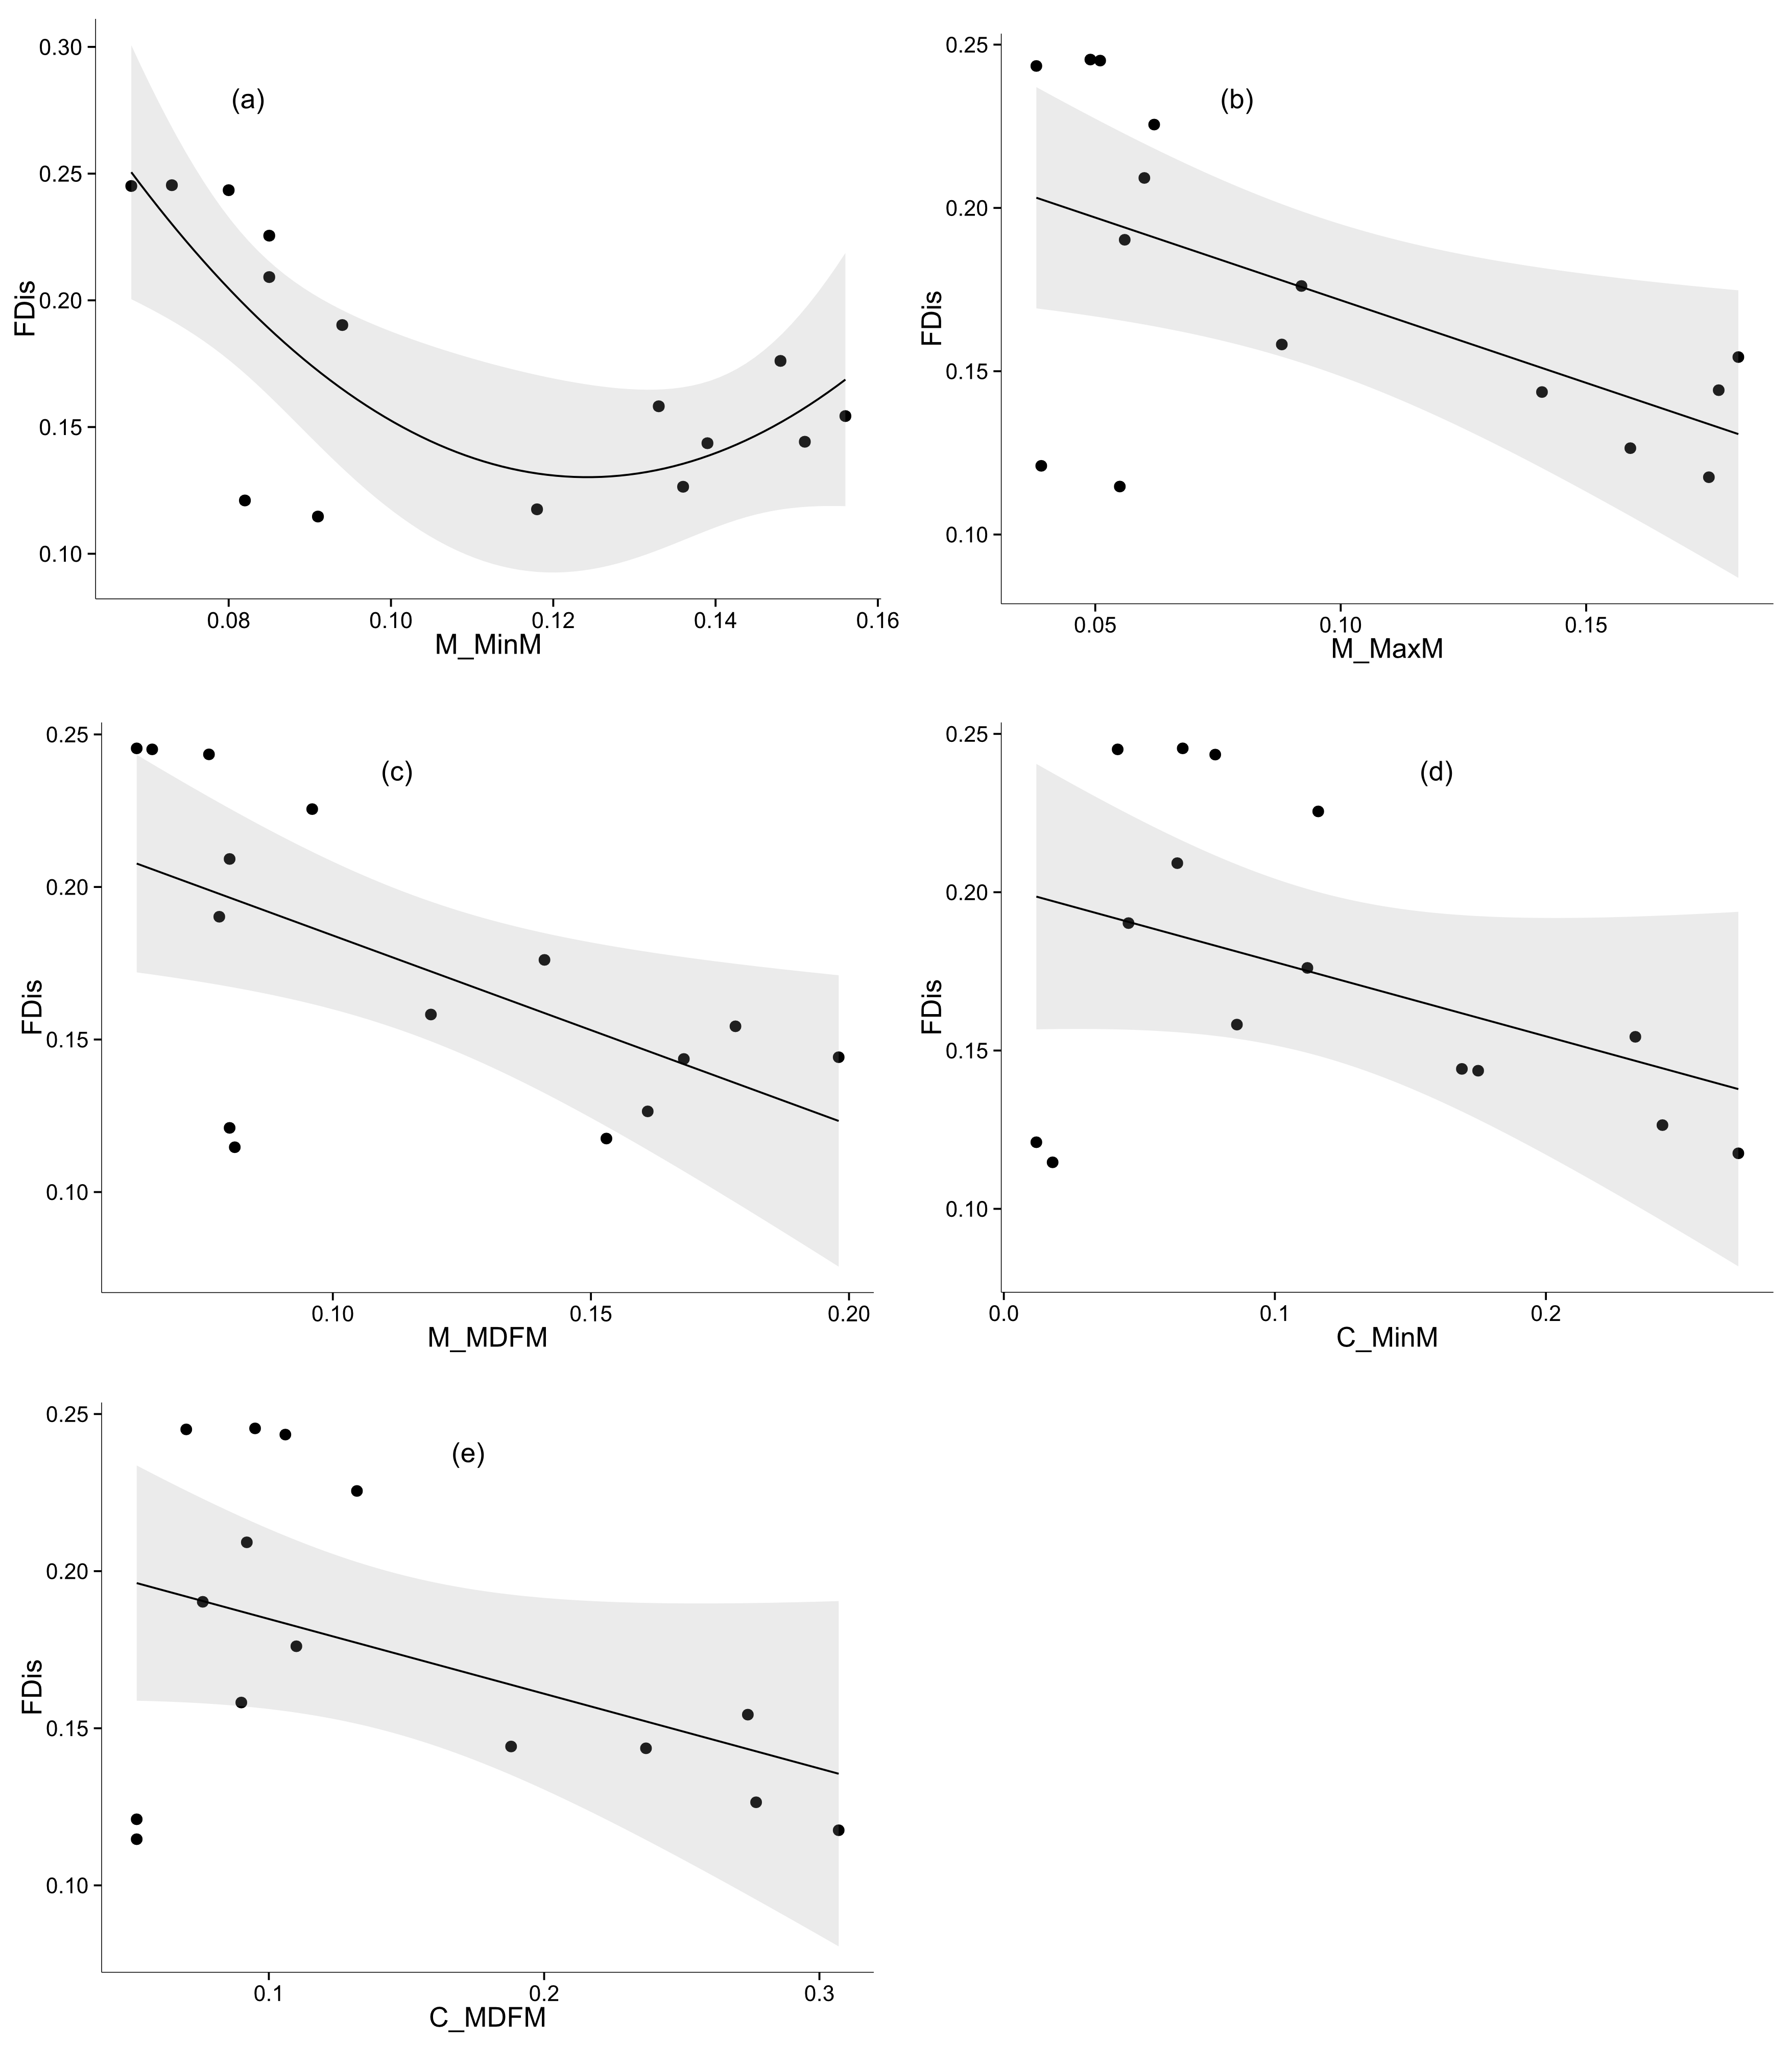
\includegraphics[width=\textwidth,keepaspectratio=true]{Ch3fig2.png} % figures can be in pdf, png, jpeg or eps format
\caption[Relationships between FDis and hydrological metrics describing variability in seasonal water availability (1).]{\small{Relationships between FDis and hydrological metrics describing (a) contingency of monthly minimum daily flow (M\_MinM), (b) contingency of monthly maximum daily flow (M\_MaxM), (c) contingency of monthly mean daily flow (M\_MDFM), (d) constancy of monthly minimum daily flow (C\_MinM), (e) constancy of monthly mean daily flow (C\_MDFM). Fitted lines depict ordinary least squares regression models. (a) is a quadratic fit, (b - e) are linear fits. Shaded areas depict the smoothed 95 \% confidence interval around the regression model. (a - c) depict significant relationships. (d - e) depict non-significant relationships (note the strong influence over the regression fit of the two points at the lower bound of FDis). Units are shown in Tables \ref{tab:Ch3_T1} and \ref{tab:Ch3_T2}.}}
\label{fig:Ch3_F2} % label for cross-referencing
\end{center}
\end{figure}   
\clearpage
This observation was corroborated by positive relationships between FDis and variability in mean daily flows for autumn (CVMDFAutumn, Fig. \ref{fig:Ch3_F3}a, adjusted p = 0.0386, R\textsuperscript{2} = 0.301), winter (CVMDFWinter, Fig. \ref{fig:Ch3_F3}b, adjusted p = 0.0278, R\textsuperscript{2} = 0.414) and spring (CVMDFSpring, Fig. \ref{fig:Ch3_F3}c, adjusted p = 0.10325, R\textsuperscript{2} = 0.327). Summer flow variability (CVMDFSummer, Fig. \ref{fig:Ch3_F3}d, adjusted p = 0.0325, R\textsuperscript{2} = 0.472) exhibited a humped relationship with FDis. Mean daily flows for both summer and spring were associated with FDis, however. This association was positive for summer (MDFMDF Summer, Fig. \ref{fig:Ch3_F3}e, adjusted p = 0.0230, R\textsuperscript{2} = 0.503) and negative for spring (MDFMDFSpring, Fig. \ref{fig:Ch3_F3}f, adjusted p = 0.0278, R\textsuperscript{2} = 0.3862).  Note that this metric actually represents the ratio of seasonal mean daily flow to the general mean of daily flow for a given river. Even though FDis was highest at sites where average flow is not associated with any particular season (low M\_MDFM), these sites still had high values for mean daily flow in summer. Pearson correlation confirms a significant negative relationship between M\_MDFM and MDFMDFSummer (Pearson's r = -0.657, p = 0.008) but not C\_MDFM and MDFMDFSummer (Pearson's r = -0.423, p = 0.1164). Summer mean daily flow may have been inflated by exceptional periods where very high average flows occurred during summer. Mean daily flow in spring, conversely, was strongly positively correlated with M\_MDFM (Pearson's r = 0.8357, p = 0.0001) and C\_MDFM (Pearson's r =0.7839, p = 0.0005), indicating that where mean daily flows in spring are high, this pattern is stable and consistent between years.

\begin{figure}[ht]
\begin{center}
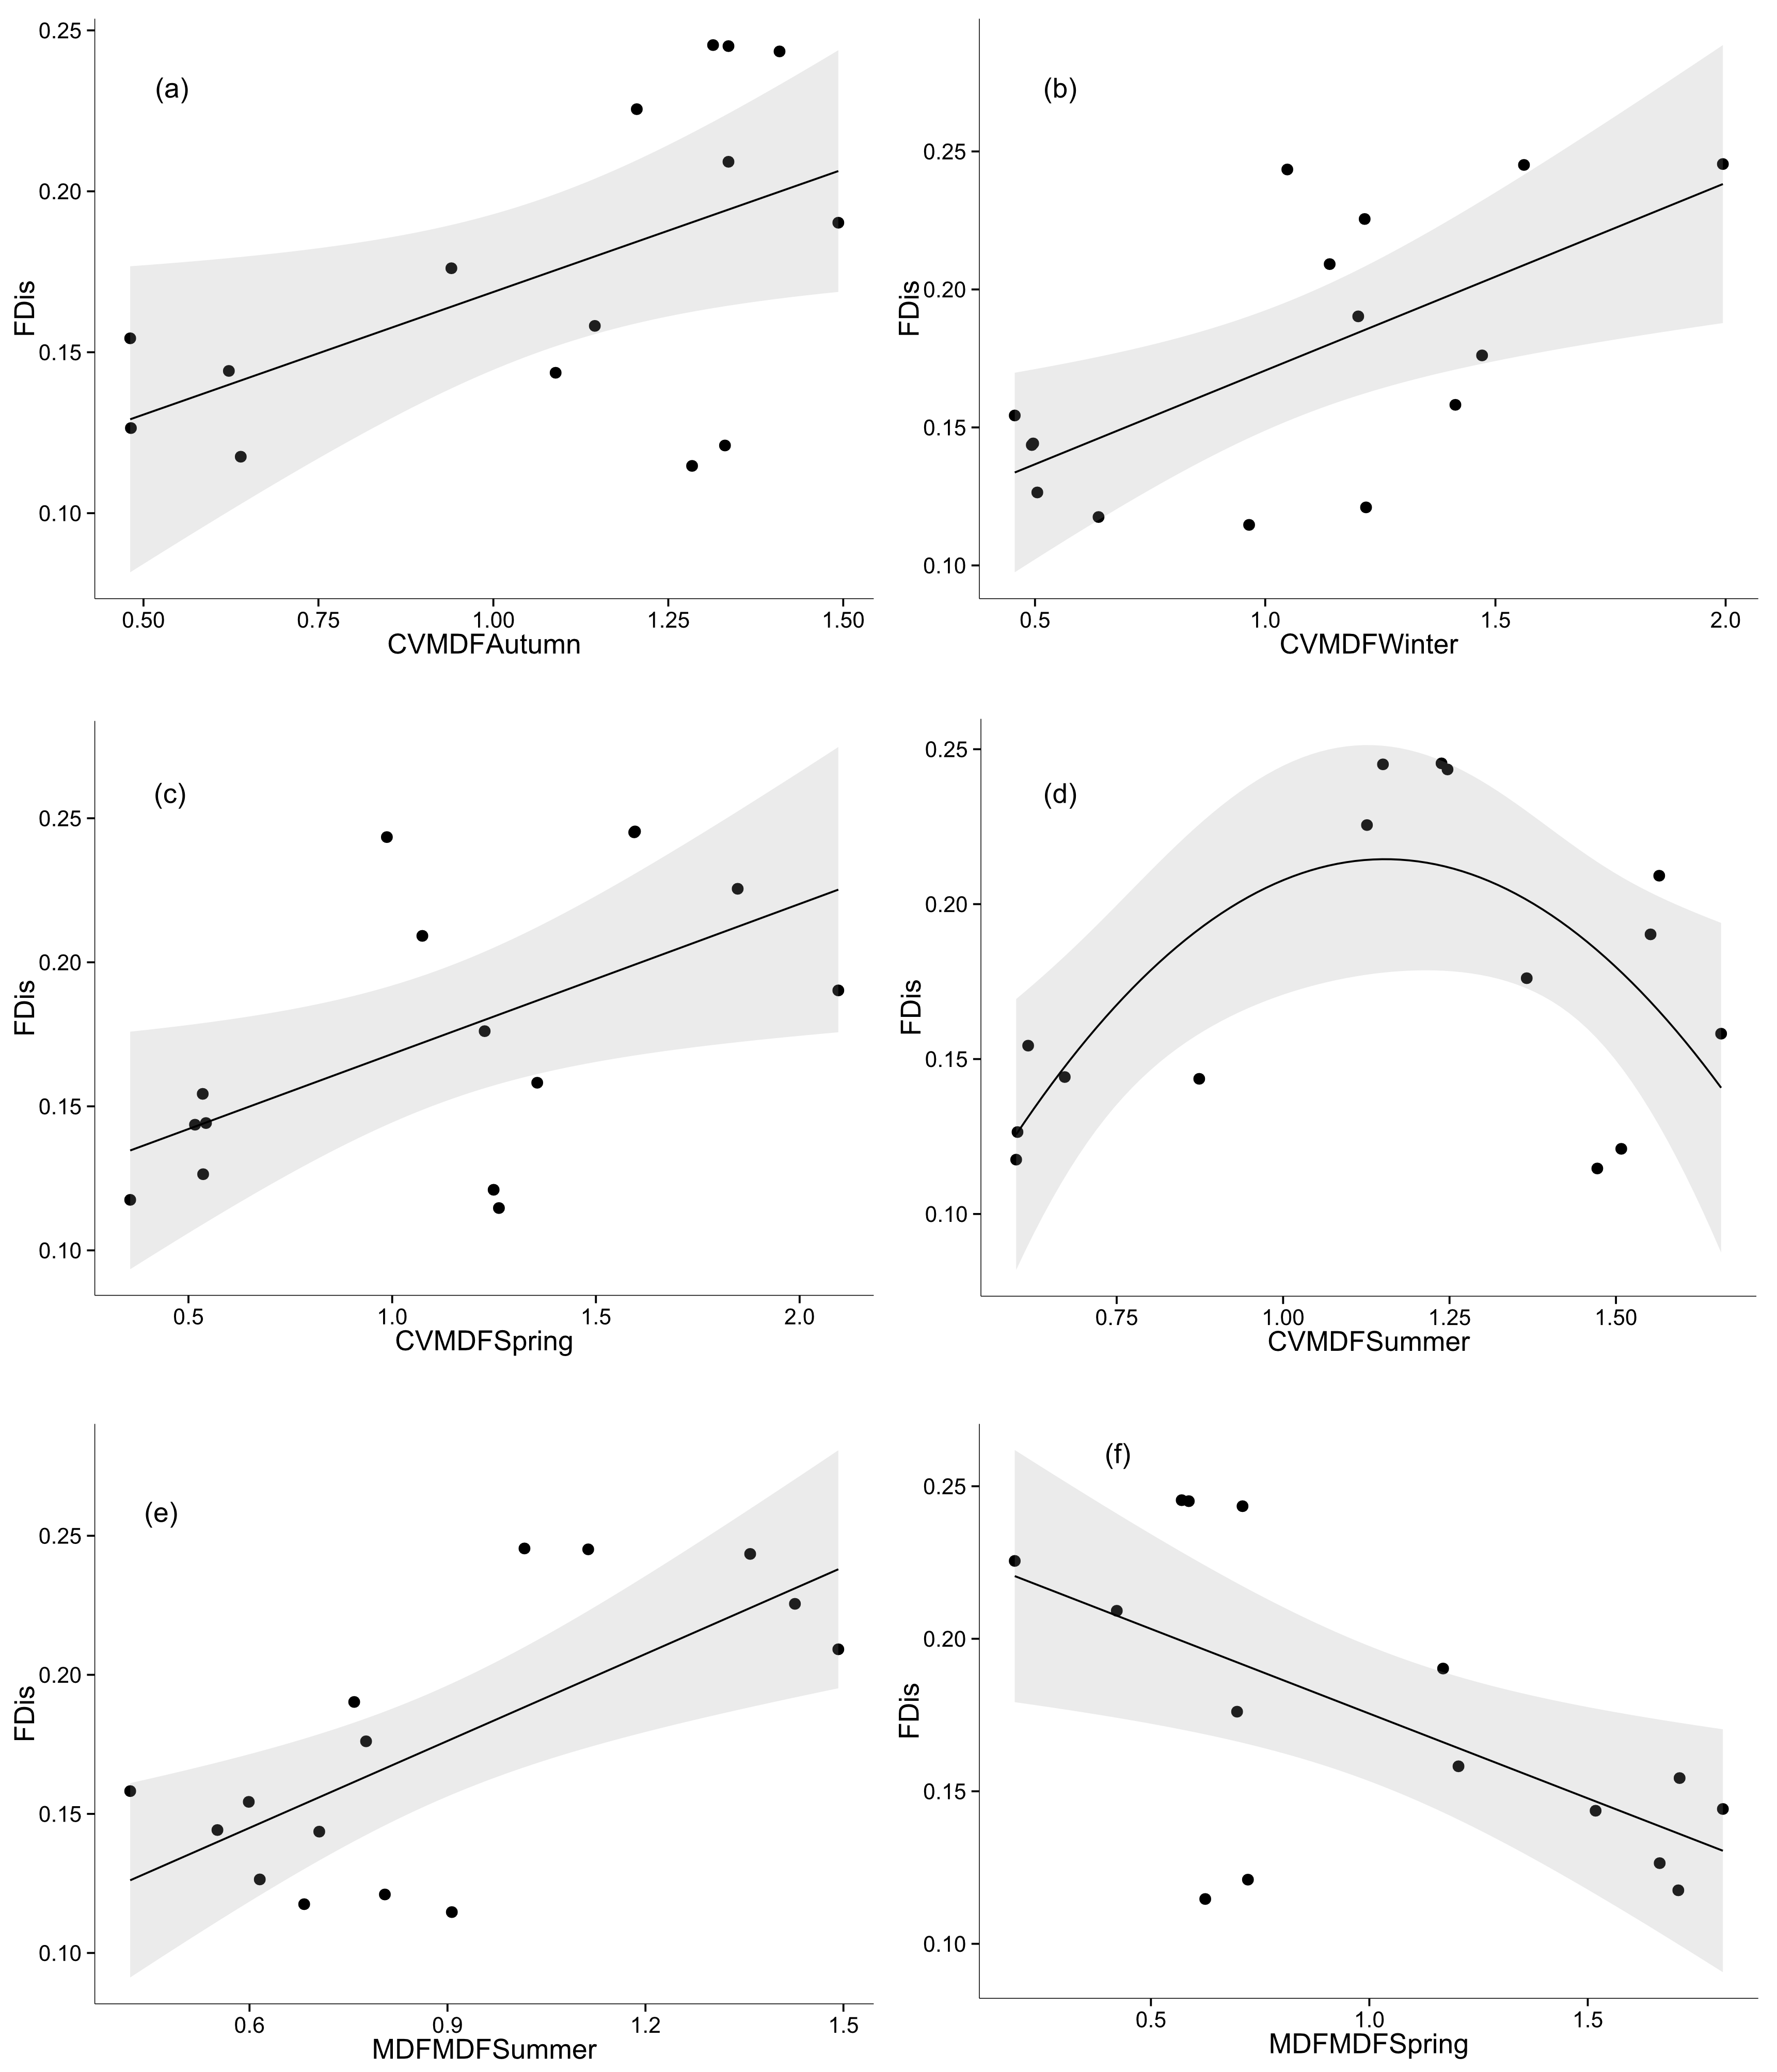
\includegraphics[width=\textwidth,keepaspectratio=true]{Ch3fig3.png} % figures can be in pdf, png, jpeg or eps format
\caption[Relationships between FDis and hydrological metrics describing variability in seasonal water availability (2).]{\small{Relationships between FDis and hydrological metrics describing (a) variability in autumn mean daily flow,(b) variability in winter mean daily flow, (c) variability in spring mean daily flow, (d) variability in summer mean daily flow, (e) mean daily flow in summer, (f) mean daily flow in spring. Fitted lines depict ordinary least squares regression models. All models are linear fits except in (d), which is a quadratic fit. Shaded areas depict the smoothed 95 \% confidence interval around the regression model.  All relationships shown are significant.  Units are shown in Tables Tables \ref{tab:Ch3_T1} and \ref{tab:Ch3_T2}.}}
\label{fig:Ch3_F3} % label for cross-referencing
\end{center}
\end{figure}   
\clearpage

\subsection{Comparisons with measures of taxonomic diversity}
Across the species used in the functional diversity analysis (i.e. present at $>$1 \% plot cover), FDis was independent of species richness (p = 0.274, F(1,13) = 1.302) and Simpson’s diversity (p = 0.513, F(1,13) =  0.454) for species included in the functional diversity analysis, but significantly associated with species richness for the full set of 327 species (p = 0.030, F(1,13) = 5.957, R\textsuperscript{2} = 0.314).

\subsection{A minimal multiple regression model to explain functional diversity according to hydrology}
We used an information theoretic procedure to select the best fitting, most parsimonious multiple regression model from the factorial set of possible models which included FDis as the dependent variable and the following independent variables: interannual variability in high flow frequency (CVAnnHSNum), interannual variability in high flow magnitude (CVAnnHSPeak) and mean daily flow during summer (MDFMDFSummer). This set of models is described in Table \ref{tab:Ch3_T3}.
\begin{landscape}
\begin{table}[ht]
\tiny
\centering
\caption[Multiple regression models with associated fitting parameters.]{\small{Multiple regression models with associated fitting parameters. * in the model formula denotes both summation as well as interaction between variables. R\textsuperscript{2} values have been adjusted for multiple regression for models using more than one variable. The optimal model according to AICc is indicated by bold typeface.}}
\label{tab:Ch3_T3}
{\tabulinesep=1.2mm
\begin{tabu}to \linewidth {lp{12cm}XXX}
\hline
\textit{\#} & \textit{Model} & \textit{adj. R\textsuperscript{2}} & \textit{AICc} & \textit{delta AIC} \\ \hline
1 & FDis {\raise.17ex\hbox{$\scriptstyle\mathtt{\sim}$}} CVAnnHSNum & 0.296 & -46.14 & 12.78 \\
2 & FDis {\raise.17ex\hbox{$\scriptstyle\mathtt{\sim}$}} CVAnnHSPeak & 0.577 & -53.79 & 5.13 \\
3 & FDis {\raise.17ex\hbox{$\scriptstyle\mathtt{\sim}$}} MDFMDFSummer & 0.503 & -51.37 & 7.56 \\
4 & FDis {\raise.17ex\hbox{$\scriptstyle\mathtt{\sim}$}} CVAnnHSNum + CVAnnHSPeak & 0.636 & -54.52 & 4.40 \\
5 & FDis {\raise.17ex\hbox{$\scriptstyle\mathtt{\sim}$}} CVAnnHSNum + MDFMDFSummer & 0.681 & -56.50 & 2.42 \\
6 & FDis {\raise.17ex\hbox{$\scriptstyle\mathtt{\sim}$}} CVAnnHSPeak + MDFMDFSummer & 0.561 & -51.71 & 7.21 \\
7 & FDis {\raise.17ex\hbox{$\scriptstyle\mathtt{\sim}$}} CVAnnHSNum * CVAnnHSPeak & 0.655 & -51.95 & 6.97 \\
8 & FDis {\raise.17ex\hbox{$\scriptstyle\mathtt{\sim}$}} CVAnnHSNum* MDFMDFSummer & 0.665 & -52.40 & 6.53 \\
9 & FDis {\raise.17ex\hbox{$\scriptstyle\mathtt{\sim}$}} CVAnnHSPeak * MDFMDFSummer & 0.566 & -48.54 & 10.39 \\
10 & FDis {\raise.17ex\hbox{$\scriptstyle\mathtt{\sim}$}} CVAnnHSNum + CVAnnHSPeak + MDFMDFSummer & 0.704 & -54.25 & 4.68 \\
11 & FDis {\raise.17ex\hbox{$\scriptstyle\mathtt{\sim}$}} CVAnnHSNum * CVAnnHSPeak + MDFMDFSummer & 0.709 & -50.14 & 8.79 \\
12 & \textbf{FDis {\raise.17ex\hbox{$\scriptstyle\mathtt{\sim}$}} CVAnnHSNum + CVAnnHSPeak * MDFMDFSummer} & 0.838 & -58.92 & 0 \\
13 & FDis {\raise.17ex\hbox{$\scriptstyle\mathtt{\sim}$}} CVAnnHSNum * CVAnnHSPeak * MDFMDFSummer & 0.944 & -48.62 & 10.30 \\ \\
\hline
\end{tabu}}
\end{table}
\end{landscape}

Model 12 was determined to be the optimal model according to AICc. Models 4, 5 and 10 were close to optimal but offered lower explanatory power according to the adjusted R\textsuperscript{2} of the model. Although Model 13 offered higher explanatory power, it was less parsimonious according to AICc and exhibited multicollinearity. Multicollinearity was determined not to be of importance for Model 12 according to variance inflation factor scores (all $<$3 on centred variables).  All terms in Model 12 were individually significant; a full summary of the model is given in Table \ref{tab:Ch3_T4}. Notably, the coefficient of the interaction term was negative, indicating a diminishing influence on FDis when values of CVAnnHSPeak and MDFMDFSummer are both high.

\begin{table}[ht]
\tiny
\centering
\caption[Regression summary for Model 12.]{\small{Regression summary for Model 12. Beta values are regression coefficents (B) standardised by the standard deviation of the term.}}
\label{tab:Ch3_T4}
{\tabulinesep=1.2mm
\begin{tabu}to \textwidth {p{6cm}XXXXX}
\hline
& \textit{B} &	\textit{SE} &	\textit{beta} &	\textit{t}	 & \textit{p} \\
\hline
CVAnnHSNum	& 0.240 & 	0.054&	0.540&	4.414&	0.001 \\
CVAnnHSPeak&	0.071&	0.026&	0.498&	2.773&	0.020 \\
MDFMDFSummer&	0.074&	0.024&	0.506&	3.056&	0.012 \\
CVAnnHSPeak * MDFMDFSummer&	-0.190&	0.060&	-0.459&	-3.186&	0.001 \\ \\ \hline 
\end{tabu}}
\end{table}

\begin{table}[ht]
\tiny
\centering
\caption[Partioning of variance in FDis as explained by optimal hydrological and climatic models.]{\small{Partioning of variance in FDis as explained by optimal hydrological and climatic models. The ‘$|$’ symbol denotes ‘controlled for’; that is, variation explained non-redundantly by a fraction.}}
\label{tab:Ch3_T5}
{\tabulinesep=1.2mm
\begin{tabu}to \textwidth {p{6cm}XX}
\hline
\textbf{Combined fractions:}	& \textit{df}&	\textit{adjusted R\textsuperscript{2}} \\
a + b (hydrology)&	4&	0.838 \\
b + c (climate)&	2&	0.629\\
a + b + c (hydrology + climate)&	6&	0.854\\
\hline
\textbf{Individual fractions:}& & 		\\
a (hydrology | climate)&	4&	0.226\\
b (shared variation)&	0&	0.612\\
c (climate | hydrology)&	2&	0.016\\
d (unexplained variation)& &		0.46\\
\hline
\end{tabu}}
\end{table}

\subsection{Do climatic or edaphic conditions explain variation in FDis that is unaccounted for by hydrological metrics?}
Of the 19 climatic variables examined, a number exhibited statistically significant univariate relationships with FDis; the quadratic function of isothermality was determined by AICc to be the optimal regression model. Of the 12 edaphic variables examined, no significant univariate relationships with FDis were found.  Variance partitioning showed that while the dominant fraction of variation explained by the two models was shared (0.612), the climatic model explained a minimal amount of non-redundant information (0.016) compared with the hydrological model (0.226), indicating a dominant influence of flow regime on functional dispersion in this study. Table \ref{tab:Ch3_T5} shows the partition table generated from this analysis.



\section{Discussion}
We surveyed vegetation communities along partly confined river systems across south-eastern Australia and found that functional diversity, as characterised by functional dispersion, exhibited strong relationships with local patterns of hydrology. The overarching pattern across these relationships can be summarised as “heterogeneous flows foster heterogeneous communities”.

This pattern is consistent with existing understanding of the processes that generate and maintain biological diversity in the riparian environment. Briefly stated, this paradigm holds that riparian biodiversity is a function of landscape complexity generated by hydrogeomorphic processes, overlain by feedback interactions between these processes and biotic components of the riparian environment \citep{Tabacchi1998, Palmer1997, Corenblit2007, Bornette2008}. Because we surveyed geomorphically homogeneous sections of sloping bank, our argument is presented under the assumption that functional diversity is a property of riparian communities at the reach scale. Influx of species from more physically complex adjacent patches, then, is responsible for the diversity we observed on these geomorphologically homogeneous sloping bank sections.

\subsection*{Relationships between functional diversity and flood intensity}

The sites surveyed in this study spanned a spectrum of flooding intensity: the 20-year average return interval (ARI) flood ranged from 18 times the mean daily flow to 210 times the mean daily flow. Higher magnitude flow events are more likely to be geomorphically effective in partly confined river systems \citep{Huang2006}. The strong positive relationship between functional diversity and 20-year ARI flood magnitude supports the supposition that disturbance retards competitive exclusion as a diversity limiting process \textit{sensu} \citet{Huston1979}. Notably, no significant relationships were found between functional diversity and metrics describing mean high flow conditions, whereas metrics describing variability had high explanatory power. Interannual variability in high flow magnitude showed the strongest relationship with functional diversity in this study. If a causal relationship exists, it could be because the average high flow magnitude determines what proportion (in terms of elevation above the main channel) of the riparian zone experiences flooding in a given year. Variability in high flow magnitude, combined with geomorphic heterogeneity, will produce variability in the time since last inundation (without significant disturbance), or combined inundation and disturbance, for a given patch of vegetation. Since flood flows also function as an important dispersal pathway for propagules \citep{Merritt2010a}, variability in high flow magnitude should influence recruitment processes in a similar manner.  Likewise, variability in the frequency of flood flows also results in variable time since last inundation or disturbance. Interannual variability in flood rise and fall rates was also positively associated with functional diversity. Overall, the combination of occasional high intensity flooding disturbance with year-to-year variability in patterning of high flow events results in a heterogeneous patch mosaic. This environmental heterogeneity provides a broad range of niches, facilitating the success of a diversity of ecological strategies \citep{Bornette2008}.

\subsection*{Relationships between functional diversity, flow heterogeneity and seasonality}
 
We can extend this framework to account for the observed relationships between functional diversity and variability in seasonal water availability.  Our sites spanned a gradient of flow seasonality: at one end, rivers exhibited weak but stable patterns of seasonality; at the other, rivers were characterised by high interannual variability and modal, seasonally inconsistent distributions of flow. Once again, communities with higher functional diversity tended to be located towards the ‘variable’ end of the spectrum. South-eastern Australian plants do exhibit characteristic species-level responses to seasonality, although there is no general coordination of growth and reproduction phenologies as in the northern hemisphere \citep{Ford1979}. Flowering times within the Myrtaceae (a dominant family in riparian plant communities of south-eastern Australia) are often staggered where species are sympatric \citep{Beardsell1993}, and growth and reproduction of riparian plants are commonly associated with the arrival of favourable conditions \citep{Woolfrey2001, Robertson2001, Siebentritt2004}. High coefficients of variation in seasonal mean daily flows may therefore act to temporarily provide species with favourable conditions according to their seasonal biology.
 
Exceptions to these patterns included the quadratic fit for variability in summer mean daily flows, with high values being associated with a reduction in functional diversity, and mean daily flow for summer, which was positively associated with functional diversity and broke the trend of associations with seasonal means being either non-significant or negative. A meta-analysis of the effect of drought on riparian vegetation showed reduced species richness and a shift towards drought-tolerant species following climate-induced increases in the intensity and duration of drought, an effect that was exacerbated by high temperatures \citep{Garssen2014}. Higher temperatures in the absence of drought were associated with higher rates of primary production. Higher mean daily flows in summer, then, potentially alleviate the water stress induced by hot weather while stimulating plant growth. We did investigate whether sites at subtropical latitudes simply had higher functional diversity than temperate sites, according to well-known latitudinal patterns of species richness \citep{Willig2003}, and found no relationship between latitude and FDis (data not presented). 

It was notable that while FDis is statistically independent of species richness, in this study functional dispersion was significantly associated with total species richness (as opposed to richness of the set of species used in the FDis analysis that were present at $>$1 \% abundance). A broad species pool therefore appears to facilitate higher functional dispersion within the dominant flora of a community, even though the richness of the dominant group of species does not necessarily determine functional diversity. It is difficult to interpret this finding, however, as adding data for rare species to the analysis would necessarily render the new value of FDis independent of total species richness.

The multiple regression model selected according to AICc explained a high proportion of variation in FDis. This model described functional diversity as a function of variability in flood frequency and magnitude, and in summer mean daily flow. The combination of flow heterogeneity with extra watering during summer appears to provide optimal conditions for functionally diverse communities. The coefficient of the interaction term between variability in flood magnitude and summer mean daily flow was significant but negative, indicating that the additive effect is subject to diminishing returns at high values of both terms. The key finding here is that these three metrics of hydrological conditions are able to account for most of the variation in FDis; data on climatic conditions and edaphic properties add very little non-redundant information to our model. We used traits in our analysis that capture a broad spectrum of ecological strategies, rather than solely traits associated with riparian specialist strategies, which might be expected to bias results towards flow response. We caveat, however, that this model does not account for the effect of plot-scale geomorphic variability on diversity, as this was controlled for in the site selection process.
 
Two sites had anomalous values for FDis that do not fit within this conceptual model of disturbance and flow variability providing high niche heterogeneity. These sites experience highly variable flows but had low functional diversity. We experimentally adjusted the abundances of dominant species at these sites and found that the low values for FDis appear to result from dominance of a single species at each site (the medium sized tree \textit{Acmena smithii} at Mammy Johnson’s Creek, and the liana \textit{Ripogonum album} at Jilliby Creek). These sites may represent cases in which species with ‘variability’ specialist strategies have become dominant. \textit{Acmena smithii} has a relatively large seed and is shade tolerant \citep{Melick1990}, but once established, develops a lignotuber and is highly resistant to drought and disturbance \citep{Ashton1976}. With respect to \textit{Ripogonum album}, there is evidence to suggest that abundance of lianas may be associated with disturbance \citep{Laurance2001} and that lianas have a competitive advantage over trees in dry conditions \citep{Swaine2007, Cai2009} (but see \citet{Nepstad2007}).

\subsection*{How generalisable are these results?}
 
Our survey covered approximately half of the range of hydrological variability present within the Australian continent; much of the lower range and middle range was captured, but highly variable dryland systems were not included \citep{Peel2004}. Our results mostly show monotonic relationships between FDis and hydrological heterogeneity, and as such do not support intermediate disturbance associated patterns found in other studies of taxonomic \citep{Bendix1997, Bendix2000, Lite2005, Corenblit2007} and functional diversity \citep{Biswas2010} of riparian plant communities. This finding is consistent with the assertion of \citet{Mouillot2013} that metrics of functional diversity should show monotonic rather than unimodal relationships with disturbance intensity. It is difficult to be conclusive on this point, however, as it is possible that we have found only the ascending half of a unimodal curve. To this end, it would be useful to survey communities that experience more extreme hydrologies, such as those in Australia’s arid regions or the monsoon tropics. Disturbance intensity and hydrological heterogeneity may not necessarily be connected in such systems. Arid zone rivers characterised by ‘all or nothing’ flow regimes may not experience the moderate flood events that generate and maintain diversity at the patch scale; for monsoonal rivers, disturbance may be similarly intense, but seasonal and interannual patterns of flow are relatively predictable \citep{Kennard2010}. In large tropical riverscapes, hydrological rhymthicity (i.e. the opposite of hydrological heterogeneity) has in fact been associated with greater richness of fish and bird taxa, and greater production in riparian forests \citep{Jardine2015}.

Unlike anthropogenic disturbances associated with agricultural land use, which have been shown to be associated with lower functional richness \citep{Pakeman2011} and lower functional redundancy \citep{Laliberte2010}, recurring hydrological disturbance appears to promote riparian plant functional diversity in this study. A similar response to natural fire regimes in the Patagonian steppe has also been observed \citep{sottile2015disturbance}. It seems reasonable to assume that the generative effect of natural disturbance on niche heterogeneity is not reproduced by typical anthropogenic disturbances.

\subsection*{Implications for river management}
 
Our findings are important from an applied river management and conservation perspective. Widespread anthropogenic river modification has altered the hydrology of river systems throughout the world, and the changing climate has the potential to exacerbate the impacts of flow modification as well as affecting unaltered river systems. A key issue with river modification is that it reduces flow heterogeneity. Dams flatten flood hydrographs (and peaks), alter seasonality and increase predictability of flows \citep{Graf2006, Singer2007}. These alterations to flow have ‘terrestrialised’ riparian areas and wetlands, reducing functional diversity and facilitating invasion by exotic terrestrial weed species \citep{Catford2011}.  Dams also interrupt hydrochorous transport of propagules \citep{Merritt2010a}, such that flood flows below dams may cause net removal of propagule material from fluvial substrates, rather than deposition. When designing environmental flows (e.g. \citet{Howell2000}), river managers typically consider magnitude, frequency and seasonality of flows. The findings in this paper agree with recent suggestions \citep{Naiman2008} that managers should also attempt to simulate flow regime variability in their designed flows.
 
Future runoff predictions are regionally specific but similarly include changes to total discharge, flow seasonality and flow variability. In regions with projected increases in climatic variability, changes to the prevalence, intensity and timing of extreme flooding or drought events can be expected \citep{Hennessy2008}. Reductions in mean summer precipitation have already occurred over large areas of Australia, coinciding with a warming of 0.4 - 0.7 \textsuperscript{o}C since 1950 \citep{Hennessy2007}. Lower average flows during hotter summers may stress riparian communities and constrain functional dispersion. Alternatively, greater climatic variability associated with future climates \citep{Hennessy2008} may promote hydrological heterogeneity in regions that were previously associated with more stable flow conditions. This may result in opening of niche space to favour opportunistic ecological strategies and promote invasion by exotic species.
 
Restoring functional diversity to pre-degradation levels may be a useful goal for riparian rehabilitation efforts along regulated or otherwise degraded river reaches. High functional diversity communities encompass a broad range of ecological strategies and should have a greater capacity to adapt to environmental change \citep{Tilman1997, Standish2014}. By working to restore functional diversity along impacted river systems, managers may increase the likelihood that riparian communities will be able to maintain critical ecosystem functions under future climates.

\subsection*{Conclusion}
 
The identification of such a strong relationship between environmental variability and functional diversity has significance for lotic ecology \citep{Palmer1997}, as well as ecology in general. Our study emphasises the importance of flooding disturbance and hydrological heterogeneity as drivers of functional diversity in riparian plant communities. These findings should be applicable to river systems in other regions and biomes characterised by moderate hydrological variability, given the profound influence of hydrology in shaping the structure of fluvial landscapes and determining the ecological strategies of plants that are able to persist and thrive in the riparian environment. Comparisons with datasets from regions with harsh but highly predictable seasonal patterns of hydrology, for example monsoonal or nival regimes, are needed to confirm this assertion. In the south-eastern Australian context, at least, alterations to flow variability and disturbance regimes by dams and the changing climate may have significant consequences for the diversity and functioning of riparian vegetation communities.

\section*{Acknowledgements}
Saskia Grootemaat, Ashley Vey, Urvashi Lallu, Julia Atkinson, Sally Lawson and Anthony Manea assisted in the field. We also wish to thank the New South Wales Parks and Wildlife Service and Parks Victoria and their dedicated officers who provided logistical advice and support. Thanks also to the landowners who were kind enough to let us work on their properties and invited us into their homes. The insight of two anonymous reviewers and suggestions the Associate Editor of Freshwater Biology, Colin Townsend, helped us to improve our draft manuscript. This research was supported by Macquarie University and an Australian Postgraduate Award scholarship to James Lawson.

\section*{Data availability}
Trait data for all species are available at \url{http://onlinelibrary.wiley.com/doi/10.1111/fwb.12649/suppinfo}.

\clearpage

%%%%% REFERENCES % this is in a new chapter due to the memoir format
\renewcommand\bibname{{References}} 
\begin{small}
\bibliographystyle{apalike}
\bibliography{library.bib}
\end{small}





\clearpage

%%%%%%%%%%%%%%%%%%%%%%%%%%%%%%%%%
% CHAPTER 4

\chapter[Environmental drivers of taxonomic and functional diversity of riparian plant communities in a modified landscape][Diversity in south-east QLD]{Environmental drivers of taxonomic and functional diversity of riparian plant communities in a modified landscape}
\newpage

\section*{Abstract}
Human populations have a profound impact on the biodiversity of riparian plant communities, and understanding the nature and mechanisms of these impacts is central to river conservation and rehabilitation. Reduction of the inherent environmental heterogeneity in riverscapes by flow modification and land-use intensification is thought to cause degradation of riparian communities.

We sampled vegetation and assembled environmental data for 20 river reaches in south-east Queensland, Australia. Plant functional trait data collated from online databases and the ecological literature were used to characterise diversity in terms of ecological strategy and functional effects. Our aim was to tease apart the environmental factors associated with taxonomic and functional trait diversity and the abundance of exotic species in riparian plant communities. We specifically tested the hypotheses that environmental heterogeneity is the dominant control on taxonomic and functional trait diversity, and that flow modification and land use intensification results in reduced diversity and promotes invasion by exotic plants.

Contrary to our expectations, hydrological metrics of environmental heterogeneity had limited power to explain patterns of species richness. Rivers which experienced seasonal, but temporally consistent flow regimes supported the most species rich communities, and modification of flow regime towards temporal consistency was also associated with greater species richness. Also against expectation, proportional abundance of exotic species increased with hydrological heterogeneity. Functional diversity metrics showed unimodal relationships with some metrics of hydrological heterogeneity, but were only weakly predicted by flow modification and showed no relationship with catchment land-use intensity.

The absence of strong linkages between the extent flow modification and metrics of functional diversity or exotic abundance suggests that use of environmental flows may not be effective as a tool for riparian rehabilitation in modified subtropical landscapes such as south-eastern Queensland.


\section*{Keywords}
Riparian, functional diversity, flow regime, environmental heterogeneity, land use, flow modification, dams

\clearpage

\section{Introduction}
Riparian ecosystems are highly biodiverse, provide important ecosystem services and are the focus of substantial management effort worldwide \citep{Naiman1993, Palmer2009}. Rapid development of catchments has changed fundamental processes which create and maintain biodiversity within riparian landscapes \citep{Nilsson2002}, and as such, riparian management often takes place within this context of catchment modification. Wholesale vegetation clearing notwithstanding, regulation of river flow regimes, catchment land-use change and invasion by exotic plant species are considered key drivers of ecological change \citep{Nilsson2000, Stromberg2007, Cooper2013}. Maintaining indigenous plant assemblages and their associated ecosystem functions, and controlling invasive species are central goals in river rehabilitation and riparian conservation \citep{Richardson2007}.

Environmental heterogeneity is one of the major factors influencing spatial patterns of species diversity \citep{Costanza2011, Stein2014}. According to classical niche-based theories of species co-existence e.g. \citet{Chesson2000}, where each niche is associated with an optimal ecological strategy, structural complexity and steep resource and energy gradients between patches promote diversity by extending niche space and reducing niche overlap. More recently, niches have been characterised in trait-space: niches and their interrelationships are described by patterns of clustering of functional traits (any morphological, physiological or phenological feature measurable at the individual level \citep{Violle2007}), the values of which are optimised to a given set of environmental conditions \citep{Adler2013}. Thus the distribution of functional traits within a community can be expected to be patterned by the degree of heterogeneity in environmental conditions present. Describing communities in traitspace dissolves species distinctions and emphasises ecological strategies: what species do within their community and how they do it. In turn, metrics of diversity derived from functional traits provide a useful complement to taxonomic diversity metrics, as they allow a mechanistic characterisation of biodiversity-ecosystem functioning relationships \citep{Hillebrand2009}. 

Much of the riparian ecology literature identifies hydrology and geomorphology as the dominant abiotic force structuring riparian ecosystems \citep{Poff1997, Bendix2000}. The spatial and temporal heterogeneity inherent in fluvial processes is considered largely responsible for the complex biogeomorphology of riparian environments \citep{Naiman2005, Corenblit2007}. Sediments are scoured and deposited, some plants are washed away while others are watered; organic matter and woody debris moves through the system and propagules are dispersed. The spatial distribution of these processes within the fluvial landscape is contingent on the magnitude and frequency of the flow events that drive erosion and deposition processes, and the resultant morphology and sedimentology of fluvial landforms produced \citep{fryirs2012geomorphic}. This subsequently determines the extent to which different surfaces/landforms are inundated under a range of different flow conditions \citep{Hughes1997}. Temporal variability in flooding patterns adds a further layer of complexity by influencing the success of plant ecological strategies for a given patch. More frequently flooded patches are likely to support graminoids and rheophytes, while succession is likely to proceed further on patches which are less frequently disturbed \citep{Corenblit2009}. Soil moisture conditions are also strongly driven by hydrology in riparian environments, with further implications for plant community assembly \citep{Nilsson2002}. 

Intermediate disturbance-type unimodal relationships between fluvial disturbance and species richness are commonly described, e.g. \citet{Bendix1997}, \citet{Bendix2000}, \citet{Lite2005}, \citet{Corenblit2007}. Unimodal relationships between environmental heterogeneity and diversity are also hypothesised to occur as a result of �microfragmentation� at high levels of heterogeneity \citep{Tamme2010}. Previous work on riparian plant communities has shown strong positive links between functional trait diversity and flow heterogeneity \citep{Lawson2015a}: relationships between functional dispersion and metrics of flow variability were mostly monotonic, with the exception of interannual variability in summertime flows, which showed a unimodal relationship.

Over half the world�s large river systems and countless smaller watercourses are affected by dams, weirs and diversions \citep{Nilsson2000, Nilsson2005}. While the effects of individual dams tend to be idiosyncratic \citep{Mackay2014}, flow regulation typically homogenises hydrographs by removing small-moderate flows, reducing flood peaks, altering seasonality and increasing predictability of flows \citep{Graf2006, Singer2007, poff2007homogenization}. Depending on the magnitude and form of change to the flow regime, flow modification may result in reduced niche complexity in downstream riparian zones \citep{Lloyd2004}. In a recent comprehensive review of ecological responses to flow modification, \citet{Poff2010} found that 152 out of 165 studies reported decreased values for recorded ecological metrics. Invasion by exotic plants in response to flood reduction often results in extensive shifts in riparian plant assemblages and reduction of both taxonomic and functional diversity \citep{Stokes2008, Merritt2010, Catford2011}. Terrestrialisation of riparian plant communities has also been described as a response to flood reduction \citep{Poff2010}. 

Human land use also has a profound effect on diversity and functioning in natural ecosystems. Land transformation for agricultural and silvicultural production, urbanisation and resulting habitat fragmentation have resulted in extensive losses of both alpha and beta diversity \citep{Vitousek1997, Gerstner2014}. This effect is often exacerbated by the entourage of exotic species brought by humans into the landscapes we occupy \citep{Vitousek1996}, with local extirpation of indigenous species \citep{Davis2003} and stifling of successional processes \citep{Catford2012a} being common outcomes of plant invasion. A recent multi-biome meta-analysis found that land-use intensification was associated with diminished functional redundancy and ability to respond to disturbance \citep{Laliberte2010}.  

Environmental homogenisation of riparian landscapes by this triad of flow modification, land-use change and exotic invasion therefore has profound implications for riparian biodiversity. The environmental flows concept posits that given a solid understanding of the hydroecology of a given riparian assemblage, restoration of riparian ecosystems on regulated rivers can be facilitated by releasing engineered flows which support indigenous plant assemblages \citep{Poff2010a}. The success of such endeavours in modified landscapes, however, is likely to be contingent on the relative contribution of flow modification and other pressures on riparian ecosystems. 

To this end, we used a functional trait diversity approach to examine vegetation responses to hydrological alteration in a modified landscape in south-east Queensland, Australia. Our aim was to tease apart the environmental factors associated with taxonomic and functional diversity and the abundance of exotic species in riparian plant communities. A set of hypotheses about environmental heterogeneity � diversity relationships guided our approach: 1.) species richness and functional diversity increase monotonically as a function of hydrological heterogeneity; 2.) abundance of exotic species declines monotonically with increasing hydrological heterogeneity, assuming greater niche heterogeneity retards competitive exclusion; 3.) species richness, functional diversity and abundance of exotic species show unimodal relationships with hydrological heterogeneity, due to microfragmentation and intermediate disturbance-type effects; 4.) species richness and functional diversity decrease along gradients of increasing flow modification and catchment land-use intensity, as an outcome of environmental homogenisation; 5.) abundance of exotic species increases along gradients of increasing flow modification and catchment land-use intensity, as an outcome of environmental homogenisation.


\section{Regional setting and hydrology}
The study was conducted across seven catchments in coastal south-east Queensland, Australia (25.82 to 28.23 \textsuperscript{o}S, and 152.35 to 153.42 \textsuperscript{o}E, see Fig. \ref{fig:Ch4_F1}). The dominant land-use in the region is agriculture, with approximately 40 \% of the area under livestock grazing, and 4 \% used for cropping. Urbanisation is also extensive, particularly along the coast. Native vegetation within conservation estate or state forest comprises 20 \% of the study area, and additional native vegetation remnants are common in steep terrain.  This study area has a subtropical climate, and is influenced by both tropical and temperate weather patterns. Little variation in temperature is present throughout the region, although mean annual rainfall varies considerably, from 800 mm in the west to 1400 mm in the eastern coastal catchments (Bureau of Meteorology 2009). The majority of rainfall is associated with summer thunderstorms between January and March, although southerly weather systems during autumn and winter are also responsible for a substantial amount of precipitation. 

Precipitation patterns are associated with high year-on-year variability, and river discharge regimes in the region are typically unpredictable, with high coefficients of variation in mean daily flow \citep{Rustomji2009, Kennard2010}. Substantial hydrological variability is represented across coastal south-east Queensland. Four of the twelve hydrological classes identified on the Australian continent by Kennard et al. (2010) are present in the area: perennial, stable baseflow; perennial, unpredictable baseflow; intermittent, unpredictable; and highly intermittent, unpredictable summer dominated.

River flow regimes throughout the study region are modified by dams, weirs, intra- and inter-basin water transfer, and unsupplemented water extraction. The majority of the dams were constructed by the mid-1970s and have a maximum capacity of less than 50,000 ML. Two substantially larger dams (Wivenhoe Dam � 1,150,000 ML and Hinze Dam � 165,000 ML) in the area were constructed during the 1980s. Mackay et al. (2014) compared historic daily discharge data with modelled predevelopment discharge data and found that flow modification by structures and diversions in south-east Queensland is diverse and system specific. Reduced flow variability is prevalent, and while increased perenniality in drier systems and altered low spell duration are also common, few other generalisations can be made about the effects of regulation on streamflows in the region \citep{Mackay2014}.

%%%% FIGURE 1
\begin{figure}[h!]
\begin{center}
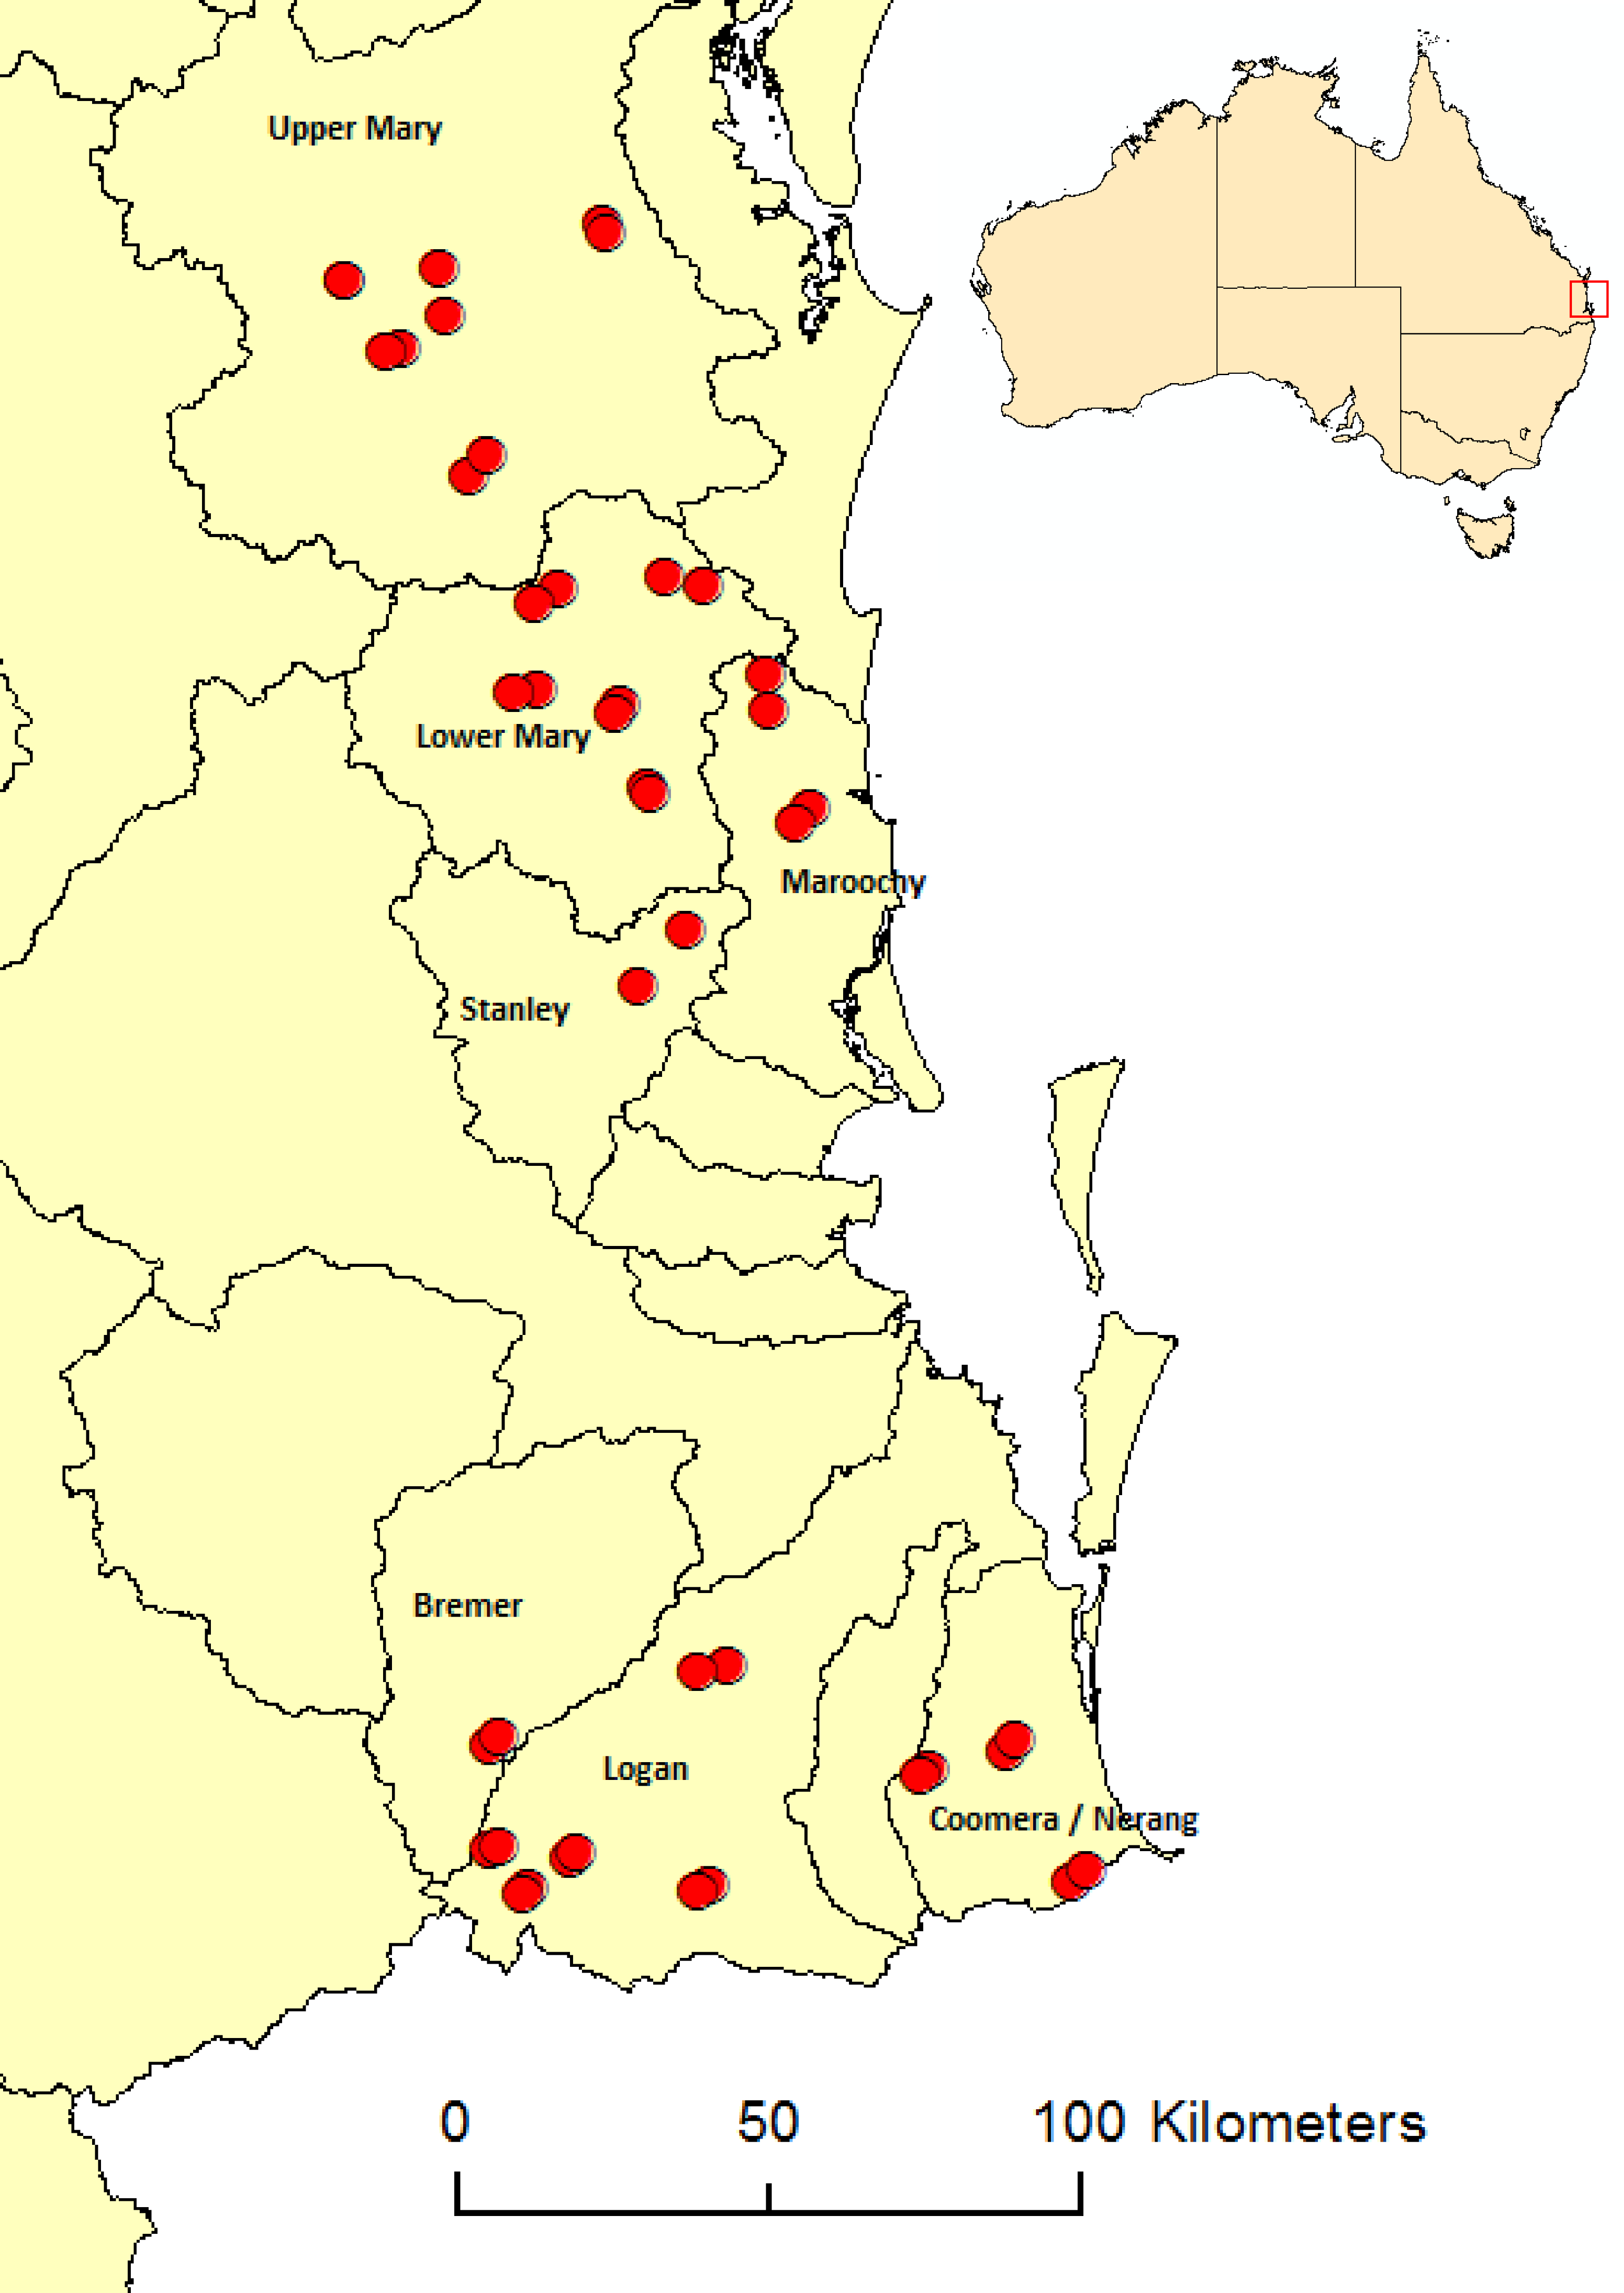
\includegraphics[width=12cm,keepaspectratio=true]{Ch4map2.png} % figures can be in pdf, png, jpeg or eps format
\caption[Study catchments and locations of field sites in south-eastern Queensland.]{\small{Study area (inset), study catchments and locations of field sites in south-eastern Queensland.}} %The caption in the square bracket is used for the table of figures. The caption in the curved brackets is the one that is printed as actual caption. 
\label{fig:Ch4_F1} % label for cross-referencing
\end{center}
\end{figure}   

\section{Methods}
The current study is an extension of a previous larger study \citep{Arthington2012}; the report describing the original study provides extensive detail not included here. Except where specified, all statistical analyses were performed using the R statistical programming environment \citep{RCoreTeam2015}, and statistical significance was thresholded at alpha $=$ 0.05.

\subsection{Site selection and vegetation sampling}
Riparian vegetation was surveyed between August and October in 2008, 2009 and 2010. Twenty river reaches were selected to sample the range of flow regime classes determined by a regional classification of flow regimes (see Mackay et al., 2014). Proximity to flow monitoring gauges with an associated recording history of $>$25 years was of primary importance. Duplicate surveys were made along each river reach as close as possible to the flow monitoring station (to give a total of 40 sites), but separated by at least 2 km. Sampling sites required 100 continuous metres of relatively intact riparian vegetation, which was not subjected to regular burning and had not been cleared in at least 20 - 30 years. Ideally sites were not currently grazed, although this restriction was relaxed somewhat given the extensive pastoral land use throughout the region. 

Three transects were randomly placed at each site, running perpendicular to the river. Additional transects were conducted at three sites, where low vegetation densities occurred. Transects extended from the water�s edge to the macrochannel bank, or to a maximum of 50 m from the water�s edge. A standard sampling area was not used due to variability in vegetation structure, channel landforms and adjacent land uses; sampling area was controlled for in subsequent analyses. Site sampling areas were typically greater than 400 m\textsuperscript{2} but ranged from 260 - 1013 m\textsuperscript{2}. All vascular plants within a 5 m band centred on the transect line were identified and counted. Species identifications were confirmed by the Queensland Herbarium. 

\subsection{Describing stream hydrology and quantifying flow regulation}
Daily discharge data for each reach were obtained from Queensland Government Department of Natural Resources and Mines (DNRM) Water Monitoring Data Portal \sloppy{\url{(https://www.dnrm.qld.gov.au/water/water-monitoring-and-data/portal)}}. 35 year time series spanning 1975 � 2009 were obtained where possible. Missing data were infilled using the Time Series Manager module in River Analysis Package \citep{marsh2003river}, using linear interpolation for periods less than 15 days, or multiple regression using data from adjacent stream gauges. One site (Reynolds Creek) had substantial periods of missing data which could not be infilled by multiple regression, as the flow at this gauge is altered by Moogerah Dam. The record for this site was truncated to exclude the periods where data was missing. The shortest remaining period (34 days) was infilled by linear interpolation. Flow data for one site (Obi Obi Creek at Kidaman) was obtained from Water Quality Accounting (Queensland DNRM) as modelled gauge data derived from a calibration model for the Mary River catchment. See \citet{Mackay2014} for further information on interpolation of hydrological data.

River Analysis Package was used to generate a set of 18 ecologically relevant hydrological metrics for each site, describing mean and interannual variability in the frequency, magnitude and duration and seasonal timing of high and low flow conditions. Table \ref{tab:Ch4_T1} provides definitions of these flow regime characteristics and describes their ecological importance and contribution to environmental heterogeneity. As a number of these metrics exhibited collinearity, we have included a principal components analysis of this data in Appendix 3a. Metrics of flow magnitude which had units ML / day were standardised by mean daily flow to allow for comparison between different river channel sizes. These metrics therefore represent ratios of flow magnitude to mean daily flow.

The extent of flow regulation at a given gauge site was characterised by the percentage deviation of each metric from the same metric generated using modelled pre-development flow data. These modelled pre-development daily discharge data were obtained from a generic integrated water quantity and quality simulation model (IQQM) developed for the region \citep{simons1996iqqm}. IQQM data were available only for the period up to 1999, so data from the timeframe 1975-1999 were used for comparison.


\begin{landscape}
\begin{tiny}
{\tabulinesep=1.2mm
\begin{longtabu} to \linewidth {m{6.5cm}m{2cm}m{2.2cm}X} 
\caption[Description of hydrological variables.]{Hydrological variables used as metrics of fluvially induced environmental heterogeneity in the riparian zone (adapted from \citep{Lawson2015a})}
\label{tab:Ch4_T1} \\
\hline
% -----------------These are headings----------------------------------%
\textit{Variable} & \textit{Abbreviation} & \textit{Units} & \textit{Description} \\ 
%
\endfirsthead
%
%\multicolumn{4}{c}%
%{{\bfseries  Continued from previous page}} \\
%\hline
%
\hline
\textit{Variable} & \textit{Abbreviation} & \textit{Units} & \textit{Description} \\ \hline
\endhead
%
%\hline \multicolumn{4}{|r|}{{Continued on next page}} \\ \hline
%\endfoot
%
%\hline
%\multicolumn{4}{|r|}{{Concluded}} \\ \hline
%\endlastfoot
%-----------Headings end---------------------------------
\hline
\multicolumn{4}{l}{\textbf{Frequency, magnitude and duration of floods and dry spells}} \\
Mean magnitude of high spells * & HSPeak & dimensionless & \multirow{12}{*}{\parbox{8.4cm}{Together, these metrics characterise the frequency, magnitude and duration of floods and dry spells. Extreme low or high flows contribute to spatial environmental heterogeneity, in that their effects (flooding disturbance, soil moisture stress) are spatially variable throughout the riparian landscape. High flow spells are periods of flow above the 95th percentile; low flow spells are periods of flow below the 5th percentile. \newline
HSPeak and LSPeak describes the mean magnitude of highest and lowest flows during high and low spells throughout the record, respectively. MDFAnnHSNum and MDFAnnLSNum describe the mean annual frequency of high and low spells. HSMeanDur and LSMeanDur describe how long flow events last. \newline
Coefficients of variation (CV) of these metrics between years characterise temporal heterogeneity in flow patterns.}} \\
Mean magnitude of low spells * & LSPeak & dimensionless &  \\
CV of all years' mean high spell magnitude & CVAnnHSPeak & dimensionless &  \\
CV of all years 'mean low spell magnitude & CVAnnLSPeak & dimensionless &  \\
Mean of all years' number of high spells & MDFAnnHSNum & year\textsuperscript{-1} &  \\
Mean of all years' number of low spells & MDFAnnLSNum & year\textsuperscript{-1} &  \\
CV of all years' number of high spells & CVAnnHSNum & dimensionless &  \\
CV of all years' number of low spells & CVAnnLSNum & dimensionless &  \\
High spell mean duration & HSMeanDur & days &  \\
Low spell mean duration & LSMeanDur & days &  \\
CV of all years' high spell mean duration & HSMeanDur & dimensionless &  \\
CV of all years' low spell mean duration & LSMeanDur & dimensionless &  \\
\tabularnewline
\hline
\newpage
\multicolumn{4}{l}{\textbf{Baseflow index}} \\
Baseflow index & BFI & dimensionless & \multirow{4}{*}{\parbox{8.4cm}{Baseflow index is calculated using the ratio of flow during average conditions to total flow. It is a useful metric of perenniality of water availability, in that it is maximised when average flow conditions dominate, and minimised when total flow is dominated by above average flow events. Thus higher baseflow systems experience more homogeneous flows.}} \\
CV of all year's baseflow index & CVAnnBFI & dimensionless &  \\[0.4cm]
& & & & \\
%\tabularnewline
\hline
%\newpage
\multicolumn{4}{l}{\textbf{Colwell's indices}} \\
Constancy of monthly minimum daily flow & C\_MinM & dimensionless & \multirow{4}{*}{\parbox{8.4cm}{Colwell's indices provide a measure of the seasonal predictability of flow events, and as such are a direct measure of temporal heterogeneity of flow patterns. \newline
Constancy (C) measures uniformity of flow across seasons, and is maximised when flow conditions do not differ between seasons. Contingency (M) is a measure of interannual uniformity in seasonal flow patterns, and is maximized when seasonal patterns of flow are consistent between years.  We generated Colwell's indices for both minimum and maximum flows conditions.}} \\
Contingency of monthly minimum daily flow & M\_MinM & dimensionless &  \\
Constancy based on monthly maximum daily flow & C\_MaxM & dimensionless &  \\
Contingency based on monthly maximum daily flow & M\_MaxM & dimensionless &  \\[0.5cm]
& & & & \\
\hline
%\newpage
\multicolumn{4}{l}{\textbf{Flow seasonality}} \\
Average mean daily dry season flow * & MDFMDFDry & dimensionless & \multirow{1}{*}{\parbox{8.4cm}{These metrics describe the average magnitude and temporal variability in mean daily flows for each season (dry = May to October, wet = November to April). Averages and coefficients of variation are calculated across yearly means. Seasonal average mean daily flows were standardised by overall mean daily flow, so actually represent the ratio of mean daily flow in a given season to the total mean daily flow.}} \\
Average mean daily wet season flow * & MDFMDFWet & dimensionless &  \\
CV of mean daily dry season flow & CVMDFDry & dimensionless &  \\
CV of mean daily dry season flow & CVMDFWet & dimensionless & \\[0.2cm] \\
\hline
\end{longtabu}}
\end{landscape}

\subsection{Other environmental variables}
Data on upstream land use were obtained via the Queensland Land Use Mapping Program (QLUMP) and dataset \citep{witte2006mapping}. These data were generated from surveys conducted in 1999 and 2006. Land use was categorised according to the Australian Land use and Management Classification version 6 \citep{BRS2002}, which differentiates conservation and low impact land uses from intensive land uses. Percentages of upstream land use were calculated as: production from relatively natural environments (forestry, grazing natural vegetation), dryland agriculture and plantations (e.g. cropping, horticulture, grazing pasture), irrigated agriculture (e.g. irrigated cropping, horticulture), conservation and natural environments (e.g. national park) and intensive uses (e.g. residential and industrial uses). We then used inverse distance weighting to weight each land use according to its proximity to the stream, following Petersen et al. (2010). 

Climate data were obtained from eMast/TERN, at a resolution of 0.01 degrees \citep{Hutchinson2014}. Bioclimatic variables representing annual trends, seasonality and extremes were calculated following the BIOCLIM framework \citep{busby1991bioclim}. The resulting set of 19 climate variables were strongly collinear, consequently PCA was used to identify a subset of six variables which represented over 90 \% of the variation in the data. Soil data were obtained from the CSIRO Soil and Landscape Grid of Australia, at a resolution of 3 arc seconds ({\raise.17ex\hbox{$\scriptstyle\mathtt{\sim}$}} 3 m) \citep{Rossel2014, Rossel2014a, Rossel2014b, Rossel2014c, Rossel2014d, Rossel2014e, Rossel2014f, Rossel2014g, Rossel2014h, Rossel2014i, Rossel2014j, Wilford2014}.

\subsection{Trait selection and dataset assembly}
We assembled a dataset of six continuous (specific leaf area, leaf area, maximum canopy height, seed mass, wood density and flowering duration) and one categorical (growth form) functional traits with which to calculate functional diversity. These traits collectively describe central trade-offs associated with ecological strategies of riparian plants (functional responses), as well as flow-on effects of species on ecosystem functioning (functional effects). Table \ref{tab:Ch4_T2} provides further description of the utility of each of these traits in characterising the functional ecology of riparian vegetation communities.

Data was taken from published literature, private and published trait datasets, and Australian flora texts. Substantial contributions were taken from the following sources: \citep{KEWseed, plantnet, zanne2009global, Wright2000, Fonseca2000, Gallagher2012a, Kooyman2013, Gleason2012} as well as from Ian Wright (pers. comm.) and Cassandra James (pers. comm.). Where multiple records for a trait were found, values were removed if they were measured at sites with an environment substantially different from south east Queensland. With the exception of maximum height, for which the highest value was used, the remaining values were averaged to provide a single value for each species-trait combination. Not all species-trait combinations could be assigned data, so to reduce biases associated with analyses of incomplete trait datasets \citep{Penone2014}, only species with fewer than 3 missing trait values (174 / 260) were retained for the analysis. The remaining missing values were imputed using a non-parametric random forests approach (missForest package for R) \citep{Stekhoven2012}. Dataset density information and imputation error estimates can be found in Appendix 3a.

\begin{landscape}
\begin{tiny}
{\tabulinesep=1.2mm
\begin{longtabu} to \linewidth {lp{5cm}XX} 
\caption[Traits included in functional diversity analysis.]{Rationale for selection of functional response and effect traits as descriptors of riparian plant community functional diversity.}
\label{tab:Ch4_T2} \\
\hline
% -----------------These are headings----------------------------------%
\textit{Trait} & \textit{Definition} & \textit{Functional responses} \& \textit{inherent trade-offs} & \textit{Functional effects} \\ 
%
\endfirsthead
\hline
\textit{Trait} & \textit{Definition} & \textit{Functional responses} \& \textit{inherent trade-offs} & \textit{Functional effects} \\  \hline
\endhead
\hline
Growth form & Categorical description of morphology: tree, shrub, woody climber, herbaceous climber, graminoid, herb. & Differential responses to mechanical and biochemical stresses associated with flooding; different strategies for coping with drought and heat stress. & Differential biogeomorphic effects on surface roughness, sediment deposition and fluvial landform cohesion. \\
Specific leaf area (SLA) & Ratio of one-sided leaf area to oven dry mass (cm\textsuperscript{2} / g). & SLA is associated with leaf construction cost, photosynthetic rate and carbon : nitrogen economics. Indicator of  ecological strategy under favourable vs. stressful conditions \citep{Wright2004}. & Affects ecosystem productivity and nutrient recycling \citep{Wright2004}. \\
Leaf area & One-sided leaf area (cm\textsuperscript{2}). & Shade tolerance (larger leaves) vs. enhanced thermal regulation ability in hot, dry conditions (smaller leaves) \citep{Cornelissen2003}. & May influence flow resistance of vegetation (and therefore fluvial erosion / deposition) when inundated. \\
Maximum canopy height & Height above ground of apical meristem (m). & Affects ability to tolerate mechanical disturbances such as flooding and maintain xylem integrity in dry conditions \citep{Westoby2006}. & Determines coarse physical structure of plant community. Surrogate for competitive ability: taller plants receive more light but must construct and maintain support structures \citep{Falster2006}. \\ \hline
Seed mass & Combined mass of the seed coat, endosperm and embryo (g). Excludes dispersal structures. & Larger seed mass confers ability to establish in unfavourable conditions \citep{Leishman2000}. Also related to seed buoyancy \citep{Carthey2015}. & Seeds may be an important food source for animals. \\
Wood density & Oven dry mass divided by green volume (g / cm\textsuperscript{3}) & Dense wood tissue confers mechanical strength, but is energetically expensive to construct. Wood density influences ability to tolerate drought stress and disturbance \citep{telewski1995wind, Preston2006, Lawson2015}. & Regulates decomposition rate; this affects nutrient cycling and determines the residency time of woody debris in the fluvial system \cite{mackensen2003decomposition}. \\
Flowering period length & Proportion of the year spent in flower (proportion, dimensionless). & Indicates species ability to respond reproductively to favourable conditions. & Flowers may be an important food source for animals. \\ \hline
\end{longtabu}}
\end{tiny}
\end{landscape}


\subsection{Calculating functional diversity, species richness and proportional abundance of exotics}
Functional richness (FRic) and functional divergence (FDiv) are complementary metrics of functional trait diversity, which together, describe the range and distribution of trait values in a community \citep{Villeger2008}. Functional evenness is also included in the framework introduced by Vill�ger et al. (2008) but has since shown limited ability to describe change in functional composition across environmental gradients \citep{Pavoine2011, Mason2012}. FRic represents the volume of the convex hull of trait values in a given community while FDiv provides information about the abundance distribution of trait values across this range.

We calculated functional richness and abundance-weighted functional dispersion (FDis) of vegetation communities at each site, using the FD package for R \citep{Laliberte2010}. Gower�s method, which scales traits by their range, was used to generate the required dissimilarity matrix, and Cailliez's correction was applied to allow for PCoA axes corresponding to negative eigenvalues and render the matrix Euclidean \citep{Cailliez1983}. We transformed FRic and FDis into standardised effect sizes (SES): SES $=$ (obs - nullExp) / sd(nullExp), where obs is the observed functional diversity value and nullExp and sd(nullExp) are the mean and standard deviation of the expected functional diversity in 999 randomized communities \citep{Gotelli2002}. The null model for comparison with FRic was generated using the trial-swap algorithm \citep{Miklos2004} in the picante package \citep{kembel2010picante} to remove dependence on species richness. The null model for comparison with FDis was generated by randomizing abundances among species but within plots (using the resamp.2s  function in spacodiR) \citep{eastman2011spacodir}, to generate a metric of pure functional divergence (FDiv). The resulting indices, FRic.SES and FDis.SES, have greater power to detect community assembly processes than their unstandardised counterparts or the metric of functional divergence defined by Vill�ger et al. (2008) \citep{Mason2013}.

To more closely comply with the assumptions of statistical tests, trait values were normalised by either log\textsubscript{10} (SLA, seed mass) or square root (leaf area, maximum height, flowering duration) transformation prior to analysis. Wood density was not transformed. Summary statistics for the trait dataset are shown in Appendix 3a.

True species richness values were estimated by rarefaction according to species accumulation across the three replicate transects taken at each site. We used the "chao1" function in the fossil package in R \citep{vavrek2011fossil} to calculate abundance-based Chao's Species Estimator \citep{chao1987}. Abundance of exotic species was calculated as the number of exotic individuals divided by the total number of individuals counted at each site.

\subsection{Constructing variance partitioning models}
We used a variance partitioning approach to assess the individual contributions of river flow regime, flow modification, land use, climate and soil properties to modelling variation in riparian plant species richness, functional diversity and exotic abundance. Exotic proportional abundance was also included as an explanatory variable for species richness and functional diversity metrics. 

The following process was used to derive an optimal set of environment-diversity models for variance partitioning analysis \citep{Legendre2007}:
We first generated minimal multiple regression models for each set of environmental variables (i.e. descriptors of flow regime, flow modification, land use etc.): for each individual dependent variable, the full set of explanatory variables was reduced to the subset which showed statistically significant (p $<$ 0.05) linear or quadratic relationships. Second order AIC was used to determine whether the linear or quadratic term better explained variation in the dependent variable (MuMIn package for R) \citep{barton2012mumin, burnham2002model}. For each set of environmental variables, variance explained by significant univariate models was partitioned by partial regression using the varpart function in R (vegan package) \citep{Oksanen2013}. Multiple regression models were derived from the combinations of variables with the highest adjusted R\textsuperscript{2} values \citep{Peres-Neto2006}. These multiple regression models optimally combine the variation explained by all significant univariate models.

The four best multiple regression models were fed into a second variance partitioning analysis, and adjusted R\textsuperscript{2} was used to estimate the proportion of variation jointly and independently explained by each environmental model.  

\section{Results}
Below we describe the patterns of variation in species richness, exotic abundance, functional richness and functional dispersion of riparian plant communities, as they relate to metrics describing river hydrology, flow modification, land use, climate and soil properties.  
Due to considerable collinearity in the environmental dataset, description of univariate relationships is generally limited here to variables selected by variance partitioning for inclusion in the final multiple regression models. Statistics for the all statistically significant univariate regression models can be found in Appendix 3b. The adj. R\textsuperscript{2} value shown in variance partitioning Venn diagrams (Figs \ref{fig:Ch4_F2}-\ref{fig:Ch4_F5}b) may not correspond directly to the sum of its fractions as represented in Figs \ref{fig:Ch4_F2}-\ref{fig:Ch4_F5}a., as negative R\textsuperscript{2} values (not shown in Figs \ref{fig:Ch4_F2}-\ref{fig:Ch4_F5}a) can result from the adjustment algorithm. All R\textsuperscript{2} values given in the text are adjusted R\textsuperscript{2}. 

\subsection{Environmental drivers of variation in species richness}
The majority of variation in species richness across the study area (0.635) could be explained by a combination of models describing flow modification, climate and soil conditions (Fig. \ref{fig:Ch4_F2}a,b). The hydrological model explained no variation in species richness independently. There was no significant relationship between total species richness per hectare and exotic species richness per hectare, and although species richness did decrease with exotic proportional abundance (R\textsuperscript{2}  $=$ 0.152) (see Appendix 3b), exotic abundance did not independently explain variation in species richness.

A weak but significant model associated richer plant communities with sites which experienced unevenly distributed patterns of minimum flows (C\_MinM, R\textsuperscript{2}  $=$ 0.098, Fig. \ref{fig:Ch4_F2}c), and where those patterns tended to be consistent between years (M\_MinM, R\textsuperscript{2}  $=$ 0.130, Fig. \ref{fig:Ch4_F2}d). Greater interannual consistency in patterns of maximum flows was also associated with richer communities (M\_MaxM, R\textsuperscript{2}  $=$ 0.207, Fig. \ref{fig:Ch4_F2}e), although a pair of sites caused the quadratic model to dip at the upper bounds of consistency. Variation in species richness was well explained by modification of seasonal consistency of minimum flow patterns (M\_MinM.mod, R\textsuperscript{2}  $=$ 0.342, Fig. \ref{fig:Ch4_F2}f), despite the relatively weak relationship between species richness and M\_MinM. A significant quadratic relationship was found between species richness and modification of seasonal consistency of maximum flow conditions (M\_MaxM.mod, R\textsuperscript{2}  $=$ 0.243, Fig. \ref{fig:Ch4_F2}g); in this case the relationship was corroborated by a similar distribution over M\_MaxM. Species richness declined with increasing interannual variability in baseflow index (CVAnnBFI.mod, R\textsuperscript{2}  $=$ 0.108, Fig. \ref{fig:Ch4_F2}h). With respect to climate, species richness was greater at sites which experienced higher rainfall in both dry (clim\_pdry, R\textsuperscript{2}  $=$ 0.417, Fig. \ref{fig:Ch4_F2}i) and wet seasons (clim\_pwet, R\textsuperscript{2}  $=$ 0.465, Fig. \ref{fig:Ch4_F2}j), and declined as temperature seasonality increased (clim\_tsea, R\textsuperscript{2}  $=$ 0.349, Fig. \ref{fig:Ch4_F2}k). Lower soil cation exchange capacity (soil\_ece, R\textsuperscript{2}  $=$ 0.373, Fig. \ref{fig:Ch4_F2}l) and soil organic carbon content (soil\_soc, R\textsuperscript{2}  $=$ 0.252, Fig. \ref{fig:Ch4_F2}l) also were associated with richer communities.

The data did not support hypothesis 1, that rivers with more heterogeneous flow regimes support communities with higher species richness. In fact, greater species richness at sites which experienced less variabilty in timing of minimum flow patterns (Fig. \ref{fig:Ch4_F2}d) supports the counter-argument - species richness here is associated with less flow heterogeneity. Hypothesis 2, that there is a unimodal relationship between species richness and flow heterogeneity, was supported by a single relationship (M\_MaxM, Fig. \ref{fig:Ch4_F2}e), although the effect of modification of M\_MaxM towards less flow heterogeneity was also strongly unimodal (M\_MaxM.mod, Fig. \ref{fig:Ch4_F2}g). These results also contradict hypothesis 4 (that species richness and functional diversity should decrease along gradients of increasing flow modification and catchment land-use intensity), given that rivers with artificially increased consistency of minimum flow patterns (M\_MinM.mod, Fig. \ref{fig:Ch4_F2}f) and lower interannual variability in baseflow index (CVAnnBFI.mod, Fig. \ref{fig:Ch4_F2}h) hosted richer plant communities.


\begin{landscape}
\begin{figure}[ht]
\centering
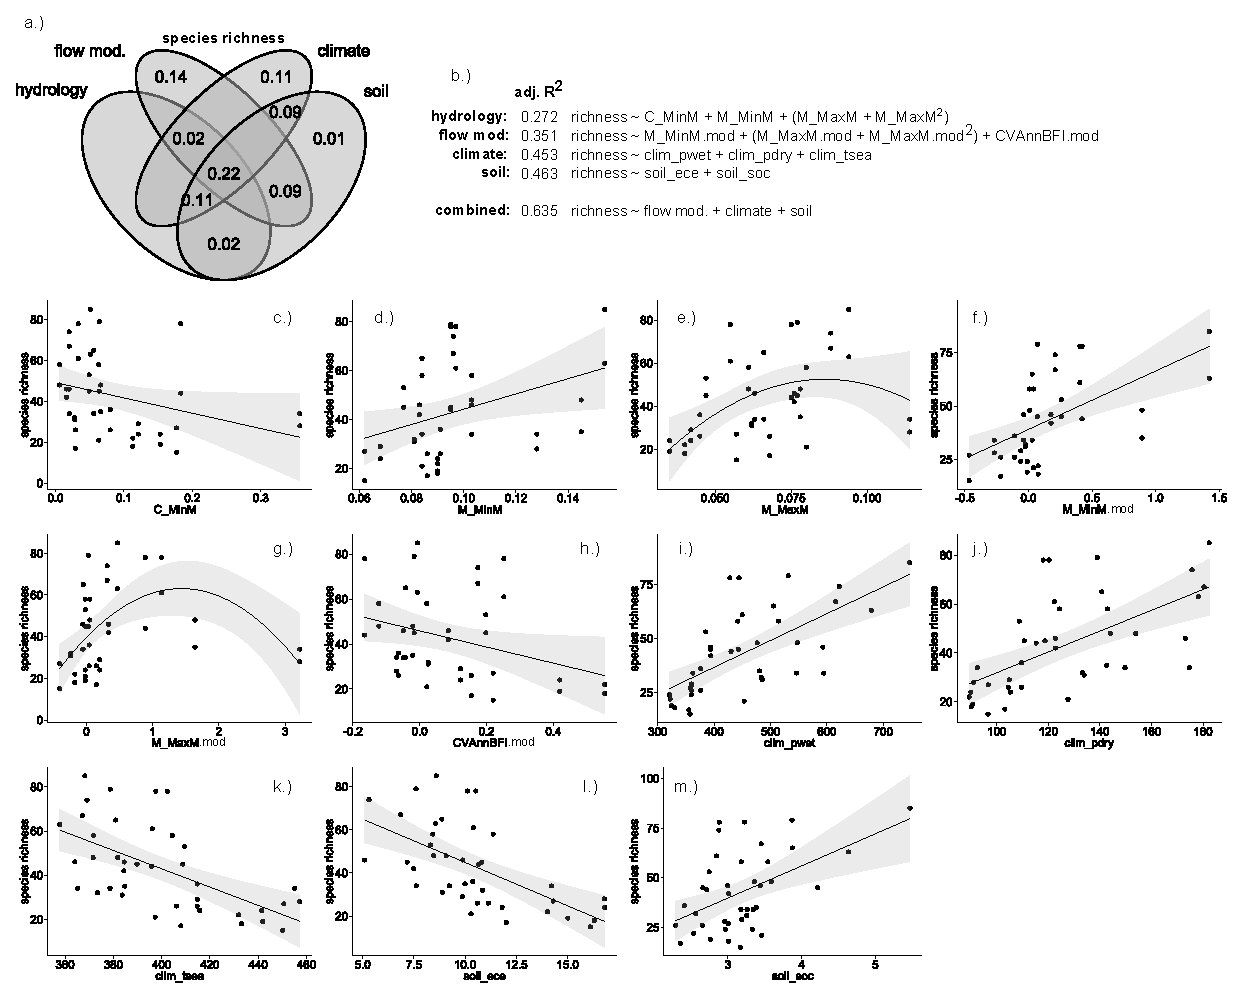
\includegraphics[height = \textheight]{Ch4speciesRichness_chao.pdf} % figures can be in pdf, png, jpeg or eps format
\end{figure}
\clearpage % insert a page break
\end{landscape}
\begingroup
\captionof{figure}[Environmental drivers of area-standardised species richness in riparian plant communities.]{\small{Environmental drivers of area-standardised species richness (units = species per m\textsuperscript{2}) in riparian plant communities. a.) variance partitioning Venn diagram. Numbers within the diagram represent adjusted R\textsuperscript{2}  (adj. R\textsuperscript{2}) values associated with each fraction of variation; b.) multiple regression models representing each set of environmental conditions, and their optimal combination. Quadratic terms are enclosed in parentheses. Selected univariate relationships between species richness and environmental variables describing c.) constancy of monthly minimum daily flows (C\_MinM); d.) contingency of monthly minimum daily flows (M\_MinM); e.) contingency of monthly maximum daily flows (M\_MaxM); f.) modification of contingency of monthly minimum daily flows (M\_MinM.mod, \% change); g.) modification of contingency of monthly maximum daily flows (M\_MaxM.mod, \% change); h.) modification of interannual variability in baseflow (CVAnnBFI);i.) precipitation in the wettest quarter of the year (clim\_pwet, mm); j.) precipitation in the driest quarter of the year (clim\_pdry, mm); k.) temperature seasonality (clim\_tsea) l.) soil effective cation exchange capacity (soil\_ece, meq per 100 g); m.) soil organic carbon content (soil\_soc, \%). Species richness is presented as the abundanced-based Chao's Species Estimator. Fitted lines depict ordinary least-squares regression models. Shaded areas depict the smoothed 95 \% confidence interval around the regression model.}}} 
\label{fig:Ch4_F2} % label for cross-referencing\endgroup
\clearpage

\subsection{Environmental drivers of functional richness (FRic.SES)}
Variation in FRic.SES was best explained by a combination of hydrological and soil models (variation explained by the combined model $=$ 0.405) (Fig. \ref{fig:Ch4_F3}a,b), of which the hydrological model gave the most explanatory power. Soil variables independently explained a small fraction of variation, and while flow modification and climatic variables were also associated with FRic.SES, neither model explained any variation independently. 

FRic.SES was distributed unimodally across gradients of interannual variability in baseflow index (CVAnnBFI, R\textsuperscript{2}  $=$ 0.170, Fig. \ref{fig:Ch4_F3}c); the modelled slope increased steeply at the lower end of the gradient but was only somewhat reduced from the peak by the top of the gradient. Greater frequency of high flow periods was associated with lower functional richness (MDFAnnHSNum, R\textsuperscript{2}  $=$ 0.142, Fig. \ref{fig:Ch4_F3}d). FRic.SES also declined as rainfall (clim\_pwet, R\textsuperscript{2}  $=$ 0.246, Fig. \ref{fig:Ch4_F3}e), soil total nitrogen (soil\_nto, R\textsuperscript{2}  $=$ 0.144, Fig. \ref{fig:Ch4_F3}f) and soil organic carbon (soil\_soc, R\textsuperscript{2}  $=$ 0.257, Fig. \ref{fig:Ch4_F3}g) increased. 

Hypothesis 1 was not supported, given that reduced functional richness was associated with increasing frequency of high flows. Hypothesis 3 was supported by a significant unimodal relationship interannual variability in baseflow (Fig. \ref{fig:Ch4_F3}c) and functional richness (delta AICc between linear and quadratic models $=$ 3.70). Although not selected for the final hydrological model, mean and interannual variability in duration of high flow periods (HSMeanDur, CVAnnHSMeanDur) also showed significant unimodal relationships with FRic.SES (R\textsuperscript{2}  $=$ 0.213, 0.182, respectively; Appendix 3b). Hypothesis 4 was not supported: we found no effect of either land use or flow modification on functional richness, except a weak relationship with modification of dry season mean daily flow (Appendix 3b). 

\begin{landscape}
\begin{figure}[ht]
\centering
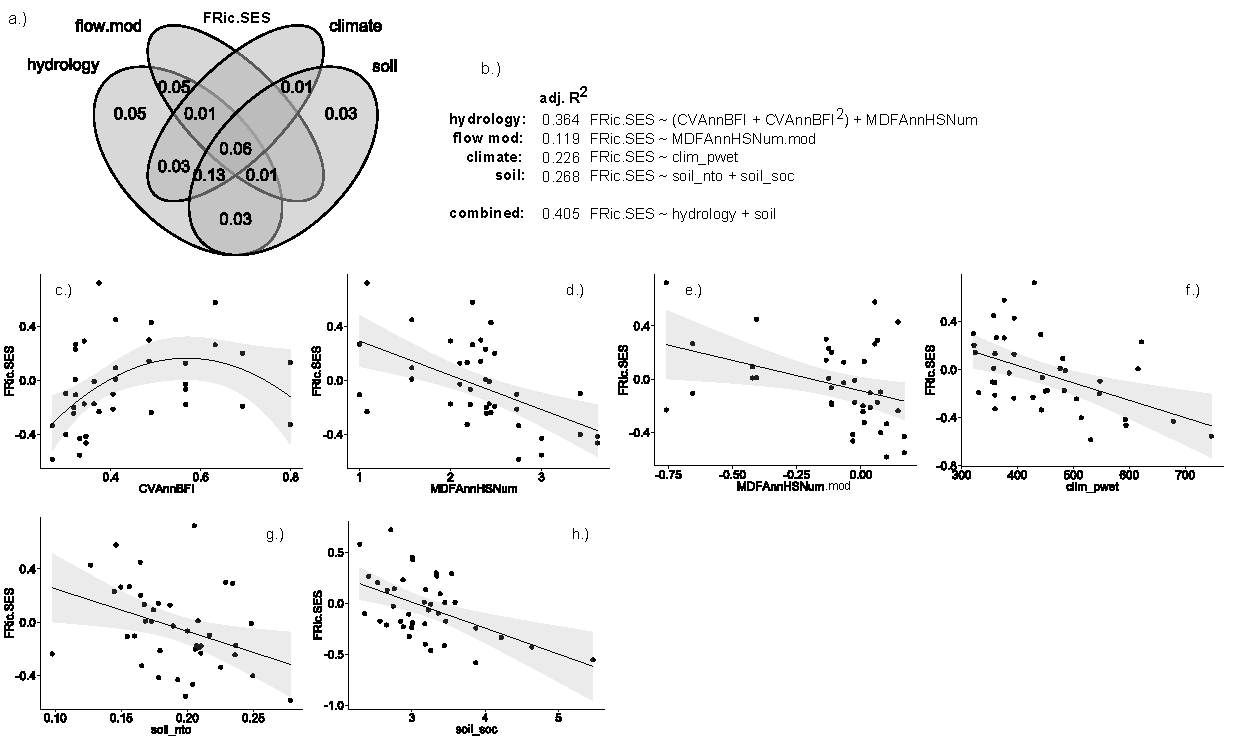
\includegraphics[height = \textheight]{Ch4FRicSES1.pdf} % figures can be in pdf, png, jpeg or eps format
\end{figure}
\clearpage % insert a page break
\end{landscape}
\begingroup
\captionof{figure}[Environmental drivers of standardised effect size functional richness (FRic.SES) in riparian plant communities.]{\small{Environmental drivers of standardised effect size functional richness (FRic.SES) in riparian plant communities. a.) variance partitioning Venn diagram. Numbers within the diagram represent adjusted R\textsuperscript{2}  (adj. R\textsuperscript{2} ) values associated with each fraction of variation; b.) multiple regression models representing each set of environmental conditions, and their optimal combination. Quadratic terms are enclosed in parentheses. Selected relationships between FRic.SES and environmental variables describing c.) interannual variability in baseflow (CVAnnBFI); d.) mean annual frequency of high flow periods (MDFAnnHSNum); e.) modification of mean annual frequency of high flow periods (MDFAnnHSNum.mod, \% change); f.) precipitation in the wettest quarter (clim\_pwet, mm); g.) soil total nitrogen (soil\_nto, \%); h.) soil organic carbon (soil\_soc, \%). Fitted lines depict ordinary least-squares regression models. Shaded areas depict the smoothed 95 \% confidence interval around the regression model.}}
\label{fig:Ch4_F3} % label for cross-referencing
\endgroup
\clearpage

\subsection{Environmental drivers of functional divergence (FDis.SES)}
FDis.SES varied substantially across the study area (3.96 standard deviations of the null distribution), and was associated with gradients of hydrology, flow modification, climatic and soil conditions. The soil model explained 0.483 of the variation in FDis.SES; hydrology, flow modification and climatic models did not independently explain further variation (Fig. \ref{fig:Ch4_F4}a,b). 

Rivers with moderate seasonality of maximum flows tended to support communities with high functional divergence (C\_MaxM, R\textsuperscript{2}  $=$ 0.321, Fig. \ref{fig:Ch4_F4}c). The entire range of FDis.SES was represented by rivers associated with highly seasonal patterns of maximum flows (C\_MaxM), however. As with functional richness, FDis.SES declined with increasing frequency of high flows (MDFAnnHSNum, R\textsuperscript{2}  $=$ 0.112, Fig. \ref{fig:Ch4_F4}d). Functional divergence also varied with flow modification affecting high flow frequency (MDFAnnHSNum.mod, R\textsuperscript{2}  $=$ 0.144, Fig. \ref{fig:Ch4_F4}e): lower flooding frequency tended to be associated with higher functional divergence. Also tracking trends observed for FRic.SES, FDis.SES declined with increasing rainfall (clim\_pwet, R\textsuperscript{2}  $=$ 0.141, Fig. \ref{fig:Ch4_F4}f), soil total nitrogen (soil\_nto, R\textsuperscript{2}  $=$ 0.111, Fig. \ref{fig:Ch4_F4}g) and soil organic carbon (soil\_soc, R\textsuperscript{2}  $=$ 0.344, Fig. \ref{fig:Ch4_F4}h).

Environmental heterogeneity (as indicated by high flow frequency) was associated with lower functional divergence (Fig. \ref{fig:Ch4_F4}d,e), opposing the prediction made in hypothesis 1, while the unimodal relationship with constancy of maximum flows (Fig. \ref{fig:Ch4_F4}c) provided some support for hypothesis 3 (delta AICc between linear and quadratic models $=$ 10.08). Scant evidence to support hypothesis 4 was found: as with FRic.SES, a weak but significant relationship was present between FDis.SES and modification of flood frequency (Fig. \ref{fig:Ch4_F4}d).

\begin{landscape}
\begin{figure}[ht]
\centering
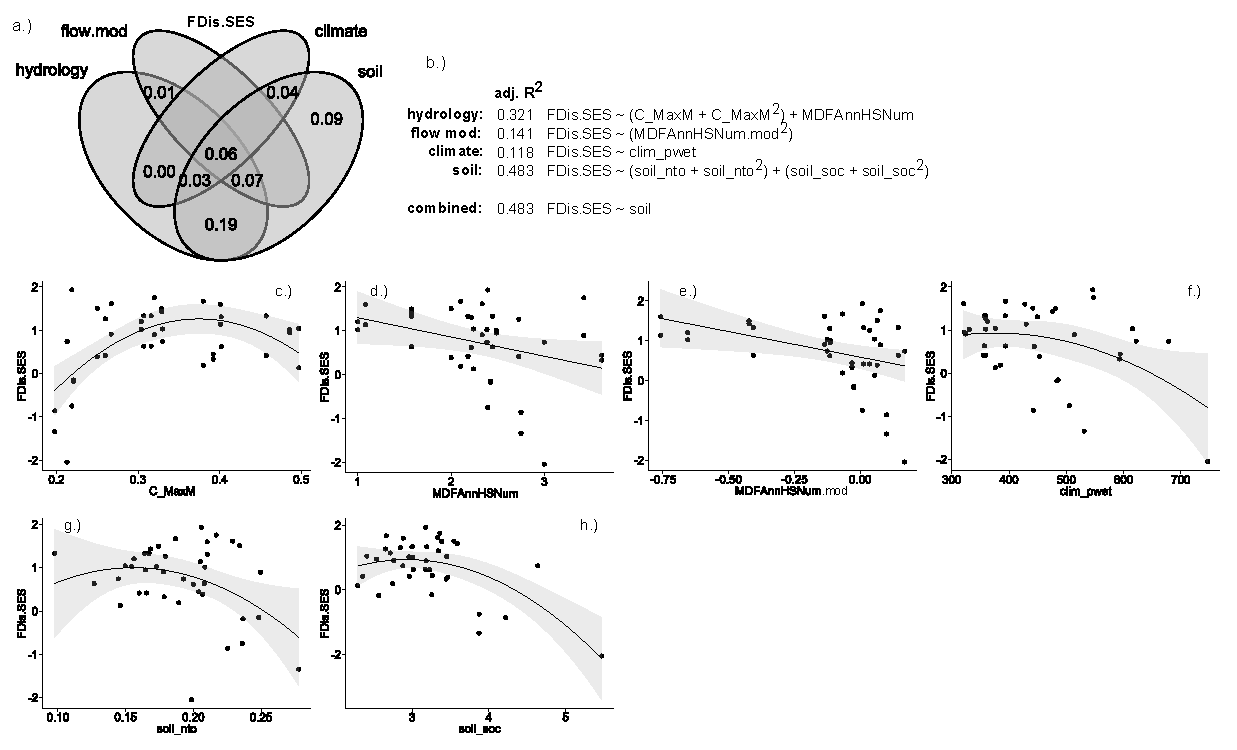
\includegraphics[height = \textheight]{Ch4FDisSES.pdf} % figures can be in pdf, png, jpeg or eps format
\end{figure}
\clearpage % insert a page break
\end{landscape}
\begingroup
\captionof{figure}[Environmental drivers of standardised effect size functional dispersion (FDis.SES) in riparian plant communities.]{\small{Environmental drivers of standardised effect size functional dispersion (FDis.SES) in riparian plant communities. a.) variance partitioning Venn diagram. Numbers within the diagram represent adjusted R\textsuperscript{2}  (adj. R\textsuperscript{2} ) values associated with each fraction of variation; b.) multiple regression models representing each set of environmental conditions, and their optimal combination. Quadratic terms are enclosed in parentheses. Selected relationships between FDis.SES and environmental variables describing c.) constancy of monthly maximum daily flows (C\_MaxM); d.) mean annual frequency of high flow periods (MDFAnnHSNum); e.) modification of mean annual frequency of high flow periods (MDFAnnHSNum.mod, \% change); f.) precipitation in wettest quarter (clim\_pwet, mm); g.) soil total nitrogen (soil\_nto, \%); h.) soil organic carbon (soil\_soc, \%). Fitted lines depict ordinary least-squares regression models. Shaded areas depict the smoothed 95 \% confidence interval around the regression model.}}
\label{fig:Ch4_F4} % label for cross-referencing
\endgroup
\clearpage

\subsection{Environmental drivers of variation in proportional abundance of exotic species}
Variation in exotic species abundance was jointly explained by hydrology, land use, soil and climatic models (0.665 of variation explained by the combined model) (Fig. \ref{fig:Ch4_F5}a,b). Hydrological models (0.581 of variation explained) and land use (0.515 of variation explained) models were dominant. Two individual metrics of flow modification had significant relationships with exotic abundance (C\_MinM.mod, R\textsuperscript{2}  $=$ 0.124; LSPeak.mod, quadratic R\textsuperscript{2}  $=$ 0.105), but these effects were strongly influenced by outlying values and the flow modification model combining these metrics explained no variation independently.

Exotic abundance closely tracked interannual variability in baseflow index (CVAnnBFI, R\textsuperscript{2}  $=$0.412, Fig. \ref{fig:Ch4_F5}c), and also rose as maximum flows became more uniformly distributed across seasons (i.e. a lack of flow seasonality) (C\_MaxM, R\textsuperscript{2}  $=$ 0.157, Fig. \ref{fig:Ch4_F5}d). We found a trough-shaped relationship between interannual variability in dry season flows and exotic abundance (CVMDFDry, R\textsuperscript{2}  $=$ 0.412, Fig. \ref{fig:Ch4_F5}e), although the lower end of the distribution was data-poor and may have been unduly influenced by values for a single pair of sites. Throughout the centre and upper ranges of the distribution, however, exotic abundance increased strongly with interannual variability in dry season flow. Exotic abundance also increased with interannual variability in high spell duration (CVAnnHSMeanDur, R\textsuperscript{2}  $=$ 0.129, Fig. \ref{fig:Ch4_F5}f). The proportion of the upstream catchment used for irrigated agricultural production was a strong positive predictor of exotic abundance (production\_irrigated, R\textsuperscript{2}  $=$ 0.37, Fig. \ref{fig:Ch4_F5}g), as was production from relatively natural environments, although somewhat less so (production\_natural, R\textsuperscript{2}  $=$ 0.232, Fig. \ref{fig:Ch4_F4}h). Exotic abundance declined as dry season precipitation increased (clim\_pdry, R\textsuperscript{2}  $=$ 0.207, Fig. \ref{fig:Ch4_F5}i), increased with soil pH (soil\_phc, R\textsuperscript{2}  $=$ 0.242, Fig. \ref{fig:Ch4_F5}j), and decreased with soil depth to hard rock (soil\_der, R\textsuperscript{2}  $=$ 0.140, Fig. \ref{fig:Ch4_F5}k).

With respect to hypothesis 2 (that abundance of exotic species should decline monotonically with increasing hydrological heterogeneity), we found the opposite of expected: hydrological heterogeneity (as measured by CVAnnBFI, CVMDFDry and CVAnnHSMeanDur) appears to be associated with higher exotic abundance. These relationships did not exhibit unimodality. Production land uses were associated with higher exotic abundance, supporting hypothesis 5 (that abundance of exotic species should increase along gradients of increasing flow modification and catchment land-use intensity).

\begin{landscape}
\begin{figure}[ht]
\centering
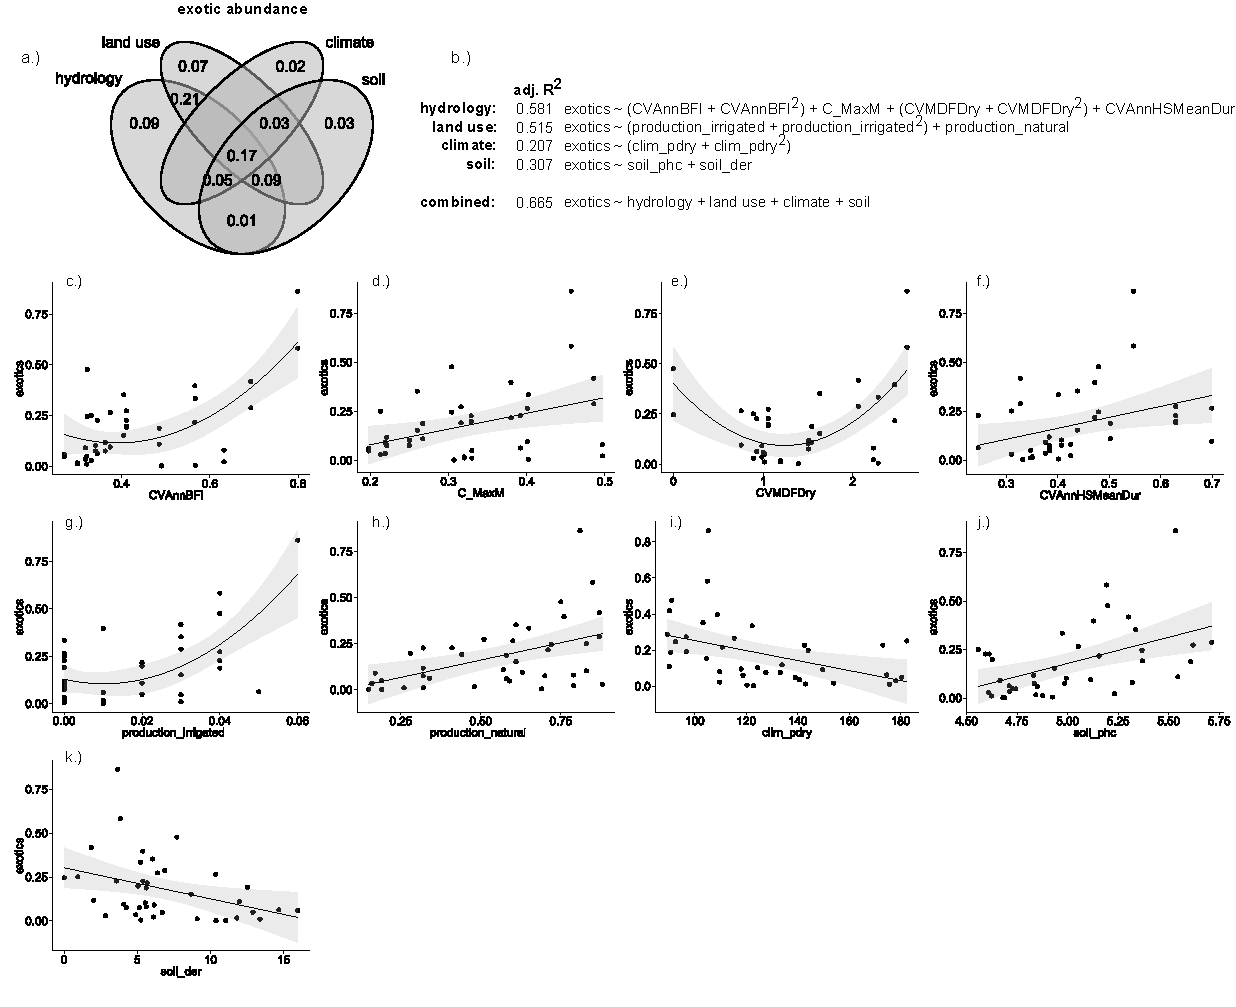
\includegraphics[height = \textheight]{Ch4exotics.pdf} % figures can be in pdf, png, jpeg or eps format
\end{figure}
\clearpage % insert a page break
\end{landscape}
\begingroup
\captionof{figure}[Environmental drivers of the proportional abundance of exotic species in riparian plant communities.]{\small{Environmental drivers of the proportional abundance of exotic species in riparian plant communities. a.) variance partitioning Venn diagram. Numbers within the diagram represent adjusted R\textsuperscript{2}  (adj. R\textsuperscript{2} ) values associated with each fraction of variation; b.) multiple regression models representing each set of environmental conditions, and their optimal combination. Quadratic terms are enclosed in parentheses. Selected relationships between exotic abundance and environmental variables describing c.) interannual variability in baseflow index (CVAnnBFI); d.) constancy of monthly maximum daily flows (C\_MaxM); e.) interannual variability in dry season mean daily flow (CVMDFDry); f.) interannual variability in mean duration of high flow periods; g.) proportion of catchment used for irrigated agricultural production (production\_irrigated, geographically weighted \%); h.) proportion of catchment used for production from relatively natural environments (production\_natural, geographically weighted \%); i.) precipitation in the driest quarter (clim\_pdry, mm); j.) soil pH (soil\_phc, \%); k.) depth of regolith (soil\_der, m to hard rock). Fitted lines depict ordinary least-squares regression models. Shaded areas depict the smoothed 95 \% confidence interval around the regression model.}}
\label{fig:Ch4_F5} % label for cross-referencing
\endgroup
\clearpage

\section{Discussion}
We proposed that generation of niche complexity by spatially and temporally heterogeneous environmental conditions is the dominant control on diversity in riparian plant communities. Under this framework, suppression of natural environmental heterogeneity by human modification of river flow regimes and catchment landscapes would result in lower diversity \citep{Poff1997, Poff2010}. This niche-oriented model of riparian plant diversity received mixed support in our study: by some metrics, species richness in fact decreased as hydrological conditions became more heterogeneous, and anthropogeneic flow homogenisation was associated with greater species richness. Although abundance of exotic species did increase with the proportion of surrounding land used for agricultural or silvicultural production, there was no relationship between exotic abundance and flow modification, and negative relationships were found with metrics of hydrological heterogeneity. The proportion of variation in functional diversity explained by environmental variables was comparatively lower than species richness or exotic abundance. Functional diversity metrics showed unimodal relationships with some metrics of hydrological heterogeneity, and declined with others. Flow modification was a weak predictor of functional diversity, and we found no effect of land use.

Given that a large proportion of variation in diversity metrics and exotic abundance explained by flow regime was co-explained by soil and climatic variables, is it possible to attribute flow regime as the dominant control on diversity? Taken individually, metrics of flow regime were the single best predictors of vegetation descriptors for FRic.SES (flood frequency, Fig. \ref{fig:Ch4_F3}d) and exotic abundance (interannual variability in dry season mean daily flows, Fig. \ref{fig:Ch4_F5}e). Species richness was best predicted by precipitation in the wet season (Fig. \ref{fig:Ch4_F2}i), while FDis.SES was best predicted by soil organic carbon content (Fig. \ref{fig:Ch4_F4}h). Variance partitioning showed that optimal models derived from flow regime metrics independently explained only a small proportion of variation in FRic.SES (Fig. \ref{fig:Ch4_F3}a)and exotic abundance (Fig. \ref{fig:Ch4_F5}a), and no independent variation in species richness (Fig. \ref{fig:Ch4_F2}a) or FDis.SES (Fig. \ref{fig:Ch4_F4}a). Extent of flow modification independently explained variation only in species richness, and changes to only a fraction hydrological metrics were important (Fig. \ref{fig:Ch4_F2}). 
As such it was not possible to give a conclusive affirmative response to this question; it is possible that relatively shallow extent of flow modification in the region over a relatively short timeframe ({\raise.17ex\hbox{$\scriptstyle\mathtt{\sim}$}}30 years) \citep{Mackay2014} did not provide the contrast required to find a consistent effect. The inherent dependency between between between climate and hydrology mean that manipulative experiments are required to confidently determine the influence of flow regime on riparian plant communities. 

Despite these limitations, we can make some interesting observations about the role of environmental heterogeneity as a driver of species richness in riparian plant communities. Contrary to expectation, sites with lower species richness were found where temporal patterns of minimum (Fig. \ref{fig:Ch4_F3}d) and maximum flows (Fig. \ref{fig:Ch4_F3}e) were less consistent between years, where interannual variability in baseflow was higher (Fig. \ref{fig:Ch4_F3}h), and also where temperature seasonality was greater (Fig. \ref{fig:Ch4_F3}k). A global meta-analysis of the ecology of tropical riverscapes showed that consistent, seasonal flow regimes support communities with higher net primary productivity and higher species richness in bird and fish assemblages than rivers with arrhythmic flow regimes \citep{Jardine2015}. Lundholm found in a meta-analysis of studies describing relationships between species richness, spatial environmental heterogeneity and energy availability, that energy availability was a better predictor of species richness than environmental heterogeneity \citep{Lundholm2009}. Temporal consistency in patterns of resource and energy availability may compete with environmental heterogeneity as a control on riparian plant diversity in this system. 

Further insight into the processes controlling riparian plant community assembly can be derived from patterns of functional diversity assembly across environmental gradients. FRic.SES represents the volume of the convex hull of trait values in a given community, as a fraction of the �expected� convex hull volume generated from randomized communities \citep{Mason2013}. FRic.SES is not weighted by species abundance and describes only the range of trait values present. FDis.SES, a pure measure of functional divergence \citep{Mason2013}, provides information about the abundance distribution of trait values across this range: functional divergence is maximised when highly abundant species are distant from the community centre of gravity in traitspace \citep{Mouchet2010}. Functional richness was unimodally related to temporal variability in baseflow index. The mechanism behind this is unclear, although following the line of reasoning developed for species richness, the effect of increased niche complexity may be offset by irregular resource availability and habitat microfragmentation as environmental heterogeneity increases \citep{Laanisto2013}.

Most communities had higher functional dispersion than predicted by the abundance-swapped null model, and a similar set of hydrological variables as FRic.SES had significant relationships with FDis.SES. FDis.SES showed a skewed, unimodal distribution across a gradient of constancy of maximum flows (C\_MaxM). Strongly negative values for several communities at the lower bound of C\_MaxM indicates functional underdispersion (i.e. environmental filtering), although the full range of variation in FDis.SES was present at low C\_MaxM \citep{Mason2013}. Variation in FDis.SES constricts as constancy increases, however, so with the exception of communities at this lower bound, communities along rivers with similar C\_MaxM tend to have similar species abundance distributions in traitspace. Interestingly, temporal variability in minimum flows (C\_MinM, M\_MinM) predicted species richness but temporal variability in maximum flows (C\_MaxM) predicted functional divergence. Compared with species richness, both FRic.SES and FDis.SES showed opposite relationships with climate and soil variables (clim\_pwet, clim\_tsea and soil\_soc, among others), indicating that trait range is not reduced in concert with species richness. The traits which do remain are clustered towards the edges of the range, producing hollowed-out community trait distributions. 

Substantial variation in exotic abundance was jointly explained by hydrological and land use models. The proportion of catchment land-use associated with irrigated agricultural production was typically low, but production from natural environments (forestry etc.) was common and dominated a number of catchments. The rationale for our hypotheses was that environmental heterogeneity should result in structural complexity of habitat and therefore limit competitive exclusion by invasive species. We found that exotic abundance was associated with more hydrologically heterogeneous sites, and a greater proportion of catchment used for forestry. Thus the combined stresses of disturbance from forestry practices and heterogeneous flows may favour novel species assemblages. It is notable that flow modification was not significantly associated with exotic abundance, given that altered flow regimes have been linked to invasion in previous studies of regulated Australian river systems \citep{Catford2011, Greet2012a} (although see \citet{Merritt2010}). It may be significant that while these former studies found flow modification exacerbated invasion primarily by herbaceous species, the most dominant invaders in this study tended to be woody trees or vines (e.g. \textit{Leucaena leucocephala}, \textit{Macfadyena unguis-cati}, \textit{Celtis sinensis}).

Environmental conditions may also have interactive effects on exotic abundance and riparian plant diversity. We originally intended to model a set of competing hypotheses about the effects of interactions between environmental conditions on diversity and exotic abundance, but the analyses described here were performed post-hoc, and the scope of possible models proved too wide to winnow down based on our limited prior understanding of the system. Future studies which explicitly accommodate tests for interactions into experimental design may provide more insight into environmental controls on diversity.

Environmental models in this study accounted for only part of the total variation in functional diversity (40.5 \% for FRic.SES and 48.3 \% for FDis.SES). In a previous study of relatively unmodified riparian plant communities in south-eastern Australia, 80 \% of variation in functional dispersion was explained by a combination of variability in flood frequency, variability in flood magnitude, and mean daily summer flow \citep{Lawson2015a}. A fraction of this variation was independently explained by climate, and none was independently explained by soil variables. In contrast, much of the variance in functional diversity metrics in the current study was jointly explained by hydrological, climate and soil models. The weak link observed between functional diversity and flow modification (Fig. \ref{fig:Ch4_F3}e, Fig. \ref{fig:Ch4_F4}e) suggests that local land management practices and land use histories, which could not be accounted for in this study, may have had a strong influence on diversity \citep{Foster2003}. Additionally, our environmental gradient analyses are based on a niche optimisation paradigm of community assembly, and do not account for neutral processes or biotic interactions \citep{Kraft2015}. Competitive interactions may play a more important role in assembly of diverse subtropical plant communities than in more austere environments dominated by abiotic forces \citep{callaway1995positive}. Indeed, as is characteristic of subtropical forests, many of the species identified in this study were not obligate riparian species (James et al., in review) and could not necessarily be expected to display traits associated with adaptation to the riparian environment. 

Despite previous findings that ecosystem multifunctionality scales linearly with functional divergence \citep{Mouillot2011}, we caution that communities which are functionally diverse but species poor may have low functional redundancy (i.e. the number of species performing similar ecological roles), which has been associated with diminished resilience to environmental change \citep{Laliberte2010}. Riparian plant communities supported by rivers with highly variable flow regimes may therefore be inherently sensitive to environmental change and exotic invasion. 

Our findings also suggest that greater runoff variability predicted to characterise future climates in south-east Queensland \citep{Hennessy2008} could have deleterious consequences for riparian plant communities. Less defined patterns of seasonality and greater variability in monthly flow patterns between years may shift assemblages towards species more tolerant of environmental variability and promote exotic invasion. Environmental flows designed to alter interannual variability in flow seasonality have the potential to significantly influence species richness in riparian communities, although their potential effects on functional diversity remain unclear. Although evidence for strong links between flow conditions and riparian plant functional diversity has been found in natural catchments of south-eastern Australia \citep{Lawson2015a}, local land use histories are likely to confound the influence of environmental flows on functional diversity in modified landscapes. 

\section*{Conclusion}

This study was motivated by a desire to provide corroboration to previous work showing strong associations between flow heterogeneity and riparian plant functional diversity \citep{Lawson2015a}, and to extend these findings into more modified landscapes. The current study demonstrates that flow regime may not necessarily be the dominant force shaping riparian plant assemblages in modified landscapes of subtropical south-east Queensland, and provides little evidence that environmental heterogeneity \textit{per se} is an important control on species richness, functional diversity or exotic abundance. Rather, generation and maintenance of diversity by rhythmic influx of energy and resources may be key \citep{Jardine2015, Lundholm2009}. The two processes are likely active together, but it remains unclear how or why one process might become dominant over the other in a given system. Species richness was associated with the extent of modification of several flow metrics, although not linearly. The absence of strong linkages between the extent flow modification and metrics of functional diversity or exotic abundance suggests that use of environmental flows may not be effective as a tool for riparian rehabilitation in modified subtropical landscapes such as south-eastern Queensland.

\section*{Acknowledgements}

The original  study upon which the present analysis is based was funded by the National Water Commission under the Raising National Water Standards (RNWS) programme, hosted and managed by the International Water Centre (IWC) and Griffith University, Brisbane. We particularly thank Anna Barnes and Stephen Mackay for all their efforts in the field. This research was supported by Macquarie University and an Australian Postgraduate Award scholarship to James Lawson. Thanks to Stuart Allen for his help in sourcing climate and soil data.

\section*{Authors' contributions}
Cassandra James designed and carried out the field component of the original study. Rachael Gallagher provided the majority of the trait data and contributed to the study design and analysis. Kirstie Fryirs and Michelle Leishman advised on the study design and analysis. James Lawson initiated and led the current project, curated the trait dataset, performed the analysis and wrote the manuscript. All authors contributed comments on the manuscript. 

\clearpage

%%%%% REFERENCES % this is in a new chapter due to the memoir format
\renewcommand\bibname{{References}} 
\begin{small}
\bibliographystyle{apalike}
\bibliography{library.bib}
\end{small}

\clearpage

%%%%%%%%%%%%%%%%%%%%%%%%%%%%%%%%%
% CHAPTER 5

\chapter[Interactive effects of waterlogging and atmospheric CO\textsubscript{2} concentration on gas exchange, growth and functional traits of Australian riparian tree seedlings][Waterlogging - eCO\textsubscript{2} interactions]{Interactive effects of waterlogging and atmospheric CO\textsubscript{2} concentration on gas exchange, growth and functional traits of Australian riparian tree seedlings}
\newpage

\section*{Abstract}
The ability to survive and thrive in repeatedly waterlogged soils is characteristic of plants adapted to riparian habitats. Rising atmospheric CO\textsubscript{2} has the potential to fundamentally alter plant responses to waterlogging by altering gas exchange rates and stoichiometry, modifying growth, and shifting resource-economic trade-offs to favour different ecological strategies. While plant responses to waterlogging and elevated CO\textsubscript{2} individually are relatively well characterised, few studies have asked how the effects of waterlogging might be mediated by atmospheric CO\textsubscript{2} concentration. 

We investigated interactive effects between elevated (550 ppm) atmospheric CO\textsubscript{2} and waterlogging on gas exchange, biomass accumulation and allocation, and functional traits for juveniles of three woody riparian tree species. In particular, we were interested in whether elevated CO\textsubscript{2} mitigated growth reduction under waterlogging, and whether this response was sustained following a refractory ‘recovery’ period during which soils were re-aerated. 

We found inconsistent effects of atmospheric CO\textsubscript{2} concentration and waterlogging status on growth, gas exchange and functional traits between species, and no evidence for a consistent effect of elevated CO\textsubscript{2} in mediating plant responses to flooding. For one species, \textit{Casuarina cunninghamiana}, elevated CO\textsubscript{2} substantially increased growth, but this effect was entirely removed by waterlogging and there was no recovery following a refractory period. 

Differential responses to combined waterlogging and elevated CO\textsubscript{2} between species may result in compositional changes to riparian plant communities and associated changes in ecosystem functioning.

\clearpage

\section{Introduction}
Woody plants play an important role in determining the physical structure of many riparian ecosystems \citep{Lawson2015}, and understanding the responses of woody riparian plants to environmental stresses is central to river rehabilitation and riparian conservation efforts. Riparian plant communities are often dominated by keystone species, and responses of such species to environmental change may have important consequences for riparian landscapes defined by their presence. Changing climatic conditions over the next century are expected to cause shifts in hydrological patterns \citep{stocker2013climate}, with changes to the prevalence and intensity of extreme flooding events predicted for many regions \citep{Hennessy2008}. Atmospheric CO\textsubscript{2} has also risen substantially over the past century, and a doubling of pre-industrial levels by 2100 is projected \citep{IPCC2014}. Flooding is already a dominant abiotic stress and an important determinant of ecological strategy for woody riparian plants \citep{Blom1996, Lawson2015}, but while a significant body of research describes the effects of elevated CO\textsubscript{2} on plants at multiple scales, little is known about how the effects of flooding might be mediated by atmospheric CO\textsubscript{2} concentration.

To thrive near stream channels, plants must navigate a trade-off between ease of access to water and stresses associated with waterlogging or inundation \citep{Naiman1993, Colmer2009}. Woody colonists of inset channel features such as bars and benches may experience repeated cycles of soil waterlogging \citep{Corenblit2009}, restricting root access to oxygen \citep{Voesenek2015}. Maintaining root respiration in low O\textsubscript{2} conditions requires switching to costly anaerobic metabolic pathways \citep{Drew1997}. The resulting reduction in respiration weakens root function, impairing uptake of water and nutrients \citep{Piedade2010, Voesenek2015} and inducing suberisation \citep{Steudle2000}. Stomatal closure may also take place following waterlogging, reducing available CO\textsubscript{2} for photosynthesis \citep{Kozlowski1984, Else2009}. Root-zone hypoxia damages roots by disrupting aerobic respiration and causing an “energy crisis” \citep{Colmer2009}; reactive oxygen species (ROS) then form as bi-products of anaerobic metabolism \citep{Santosa2007}, and  subsequent re-aeration further increases ROS production \citep{Steffens2013}. Production of toxic ions by microbes under anoxic soil conditions causes additional stress to roots \citep{Blom1996}. Waterlogging may also impair rhizomicrobial nodule formation and activity, resulting in reduced nutrient uptake \citep{Dawson1989, Shimono2012}. The degree to which this combination of stressors influences plant growth is ultimately determined by species’ ability to mobilise physiological and morphological responses which mitigate damage \cite{Bailey-Serres2008}.
  
As with waterlogging, atmospheric CO\textsubscript{2} concentration is known to affect plant physiology and growth by altering the fundamental economics of carbon, water and macronutrient uptake and use \citep{Poorter2003a, Wang2012, Reich2014}.  Individual species responses are variable, but photosynthetic CO\textsubscript{2} assimilation in C3 plants tends to increase under elevated CO\textsubscript{2} (eCO\textsubscript{2}) \citep{Curtis1996}. Stomatal conductance is also typically reduced \citep{Ainsworth2007}, with attendant gains in water use efficiency \citep{Holtum2010, Keenan2013, VanderSleen2014}. Biomass accumulation in response to eCO\textsubscript{2} may be enhanced \citep{Wang2012}, but this depends on the availability of water and macronutrients \citep{Korner2006, Manea2014, Reich2014}. Increased allocation of biomass to roots occurs under eCO\textsubscript{2} \citep{Nie2013} and this effect is interactive with environmental stresses such as drought or low soil fertility \citep{Wang2010}. Increased rates of production and turnover of fine roots under eCO\textsubscript{2} have been shown in the field, which has important implications for nutrient cycling and ecosystem functioning \citep{Pregitzer1995, Pregitzer2000, Matamala2000, Lipson2014}. eCO\textsubscript{2} is also known to affect functional traits indicative of positions along economic spectra (\textit{sensu} Reich 2014). Reduction in specific leaf area (SLA) under eCO\textsubscript{2} may be linked to accumulation of non-structural carbohydrates in leaves \citep{Poorter2003a, Bader2010}. Alteration of traits reflecting economic trade-offs is of particular significance at the seedling stage, as functional traits of trees are most strongly adapted to the regeneration niche \citep{Poorter2007}.

Taken individually, waterlogging and elevated atmospheric CO\textsubscript{2} concentration appear likely to exert opposing effects on plant growth. The possibility that eCO\textsubscript{2} may mitigate growth reduction under waterlogging warrants investigation of the interactive effects of these two important environmental variables. Literature describing interactive effects of atmospheric CO\textsubscript{2} concentration and waterlogging or flooding on plant growth is sparse, and findings thus far present an inconsistent picture. eCO\textsubscript{2} stimulated biomass production in waterlogged (water table at -10 cm) but not inundated (water table at +5 cm) juveniles of the flood-tolerant tree species \textit{Taxodium distichum} \citep{Megonigal2005}. Increased photosynthesis under eCO\textsubscript{2} was not reduced by inundation. This effect was attributed to the increased metabolic cost of maintaining roots under low O\textsubscript{2} conditions. In the same study, inundation had no effect on eCO\textsubscript{2} stimulation of photosynthesis or biomass production of the aquatic herbaceous species \textit{Orontium aquaticum}.  The opposite response was found for a highly flooding tolerant Amazonian tree: waterlogged Senna reticulata grown in open top chambers showed greater increment in biomass under eCO\textsubscript{2} \citep{Arenque2014}. Finally, no evidence for an interaction between CO\textsubscript{2} concentration and waterlogging status was found on growth or stomatal conductance in soybean \citep{Shimono2012}. To our knowledge, no studies have investigated the effects of eCO\textsubscript{2} on recovery from waterlogging. Ability to recover following stress events may be a better indicator of fitness than tolerance of the stress \citep{Gutschick2003}, and for waterlogged plants, generation of reactive oxygen species following re-aeration is likely to be a significant additional stress \citep{Drew1997}. 

The objective of this study was to investigate interactive effects between eCO\textsubscript{2} and waterlogging on gas exchange, biomass accumulation and allocation, and functional traits for riparian tree species. In particular, we were interested in whether eCO\textsubscript{2} mitigated growth impairement under waterlogging, and whether this response was sustained following a refractory ‘recovery’ period during which soils were re-aerated. We also investigated two hypothesised mechanisms by which such an interactive effect might occur: a.) higher water use efficiency under eCO\textsubscript{2} \citep{Holtum2010} facilitates photosynthesis in plants with anoxia-impaired root functionality by lowering the water cost of carbon assimilation; b.) eCO\textsubscript{2} facilitates biomass recovery by increasing the rate of fine root production during the recovery period \citep{Pregitzer1995}.  

\section{Methods}
We selected three riparian tree species native to south-eastern Australia for this study. \textit{Casuarina cunninghamiana subsp. cunninghamiana} and \textit{Eucalyptus camaldulensis subsp. camaldulensis} dominate many riparian environments in south-eastern Australia; \textit{Acacia floribunda} is also common in this region. Table \ref{tab:Ch5_T1} provides further information on the biology and ecology of these species.

\begin{threeparttable}[h!]
\tiny
\centering
\caption[Biological and ecological attributes of study species.]{\small{Biological and ecological attributes of study species.}}
\label{tab:Ch5_T1}
\begin{tabularx}{\textwidth}{XXXX}
\hline
 & {\textit{Acacia floribunda}} & {\textit{Casuarina\newline cunninghamiana subsp.\newline cunninghamiana}} & {\textit{Eucalyptus\newline camaldulensis subsp. camaldulensis}} \\ \hline
Family & Fabaceae & Casuarinaceae & Myrtaceae \\
Distribution & Coastal areas of eastern Australia\textit{\textsuperscript{1}} & Eastern NSW and QLD, Australia. Other subsp. in Gulf of Carpentaria and Papua New Guinea\textit{\textsuperscript{1}} & Inland riparian areas throughout south-eastern Australia. Other subsp. distributed throughout continental Australia\textsuperscript{1} \\ \
Morphology & Erect or spreading shrub or tree, 3–8 m high\textit{\textsuperscript{1}}. Rooting depth 2 m +\textit{\textsuperscript{2}} & Erect tree, 15–-35 m high\textit{\textsuperscript{1}}. Rooting depth to 8 m\textit{\textsuperscript{2}} & Large, spreading tree, 30+ m high\textit{\textsuperscript{1}}. Rooting depth 10 m+ \textit{\textsuperscript{2}} \\ \
Habitat & Facultative rheophyte. Found in sclerophyll forest, particularly along watercourses and in sandy alluvial soils. Typically on channel banks and raised within-channel features\textit{\textsuperscript{1}} & Obligate rheophyte. Found along permanent watercourses, on substrates ranging from sand to large cobbles. Often found on bars, benches and channel islands\textit{\textsuperscript{1}} & Obligate rheophyte. Found on deep, rich alluvial soils, on banks and flood plains associated with large, permanent water bodies\textit{\textsuperscript{1}} \\ 
Community status & Common\textit{\textsuperscript{1}} & Dominant\textit{\textsuperscript{1}} & Dominant\textit{\textsuperscript{1}} \\
Nitrogen fixing ability & Nodulated with Rhizobium\textit{\textsuperscript{3}} & Nodulated with Frankia\textit{\textsuperscript{4}} & None \\
Biogeomorphic effects & Colonist of fresh geomorphic substrates\textit{\textsuperscript{5}} & Ecosystem engineer. Rapid, en mass colonisation and stabilisation of fresh geomorphic substrates. Established trees stabilise banks and in-channel features\textit{\textsuperscript{2}} & Ecosystem engineer. Established trees define physical structure of riparian landscapes. Highly effective at mitigation of flooding-induced landform mass failure\textit{\textsuperscript{2}} \\ \hline
\end{tabularx}
  \begin{tablenotes}
    \item \textit{\textsuperscript{1}} \cite{plantnet}, \textit{\textsuperscript{2}} \cite{Hubble2010}, \textit{\textsuperscript{3}} \cite{roughley1987acacias}, \textit{\textsuperscript{4}} \cite{Dawson1989}, \textit{\textsuperscript{5}} J. Lawson personal field observations
  \end{tablenotes}
\end{threeparttable}

\clearpage

\subsection{Experimental procedure}
We used a fully factorial design comprising two CO\textsubscript{2} treatments (ambient and elevated), and three waterlogging treatments (non-waterlogged control, waterlogged and waterlogged then re-aerated for a refractory period), with 8 replicates per treatment combination per species. We measured plant physiology (photosynthetic rate, A; stomatal conductance, G\textsubscript{s}; and instantaneous water use efficiency, WUE) as well as biomass, biomass allocation and tissue density traits indicative of ecological strategy and position along economic spectra \citep{Reich2014}.

Plants were grown individually in pots constructed from 90 mm by 700 mm (4.3 L capacity) sections of PVC pipe with drilled endcaps, containing a commercially sourced 80/20 mixture of river sand and soil (Australian Native Landscapes, North Ryde, NSW, Australia). The bottom 2 cm of each pot was filled with gravel (~1 cm particle size) to promote free drainage. 2.5 g L\textsuperscript{-1} of time-release fertiliser granules (NPK 19.1, 0, 11.9, Yates Australia, Padstow, NSW, Australia) was mixed evenly through the soil medium.

Seeds were obtained from a commercial supplier (Nindethana Seed Service, Albany, WA, Australia) and germinated on moist tissue paper in trays at ~20 \textsuperscript{o}C. Following cotyledon emergence, four seedlings were transplanted into each growing pot. Germination was staggered by species to ensure all seedlings were transplanted at the same stage of development (radicle just emerged) within 48 hours. After two weeks of growth, plants were thinned to retain a single, medium sized individual.

Plants were grown in glasshouses at Macquarie University, in Sydney, Australia, between June and November, 2014. Pots were supported by wire mesh on trolleys; pot positioning on trolleys was randomised with respect to species, and trolleys were rotated weekly to offset potential microclimatic effects associated with position within each glasshouse. Two levels of CO\textsubscript{2} treatment (380-400 ppm and 530-570 ppm) were used in two replicate glasshouses per level. These CO\textsubscript{2} ranges were monitored and maintained using an automated gas delivery system (Canary Company Pty Ltd, Lane Cove, NSW, Australia). The lower range corresponds to the ambient atmospheric CO\textsubscript{2} concentration, while the higher range reflects the predicted atmospheric CO\textsubscript{2} concentration in 2050 \citep{IPCC2014}. Temperature was maintained between 16 and 28 \textsuperscript{o}C. Plants were watered by a misting sprinkler system three times daily and provided with supplementary hand watering every 3-4 days to maintain constant soil moisture levels between pots. Trolleys were swapped between replicate glasshouses monthly.

Waterlogging was initiated after 90 days of plant growth and lasted 24 days, in order to simulate a significant flooding event and to allow time for morphological adaptation to manifest. Plants were randomly assigned to “control”, “waterlogged” and “recovery” treatments. “Waterlogged” and “recovery” plants were waterlogged by immersion to within 10 cm of the soil surface in 450 L plastic tubs filled with water. The black tubs were covered with white polythene sheeting to reduce heat absorption. Photosynthetic rate and transpiration rate of plants assigned to the “waterlogged” treatment were measured at the end of the waterlogging period, after which they were harvested. Tubs were drained following the waterlogging period, and “control” and “recovered” treatment plants were grown for a further 23 days before measurement and harvesting.

Photosynthetic rate (CO\textsubscript{2} assimilation rate), stomatal conductance and transpiration rate of the newest fully developed leaf were measured for four plants per treatment between 9 am and 12:30 pm using a Li-Cor 6400XT infrared gas analyser (Li-Cor Inc., Lincoln, NE, USA). Photon flux was set to 1500 µmol m\textsuperscript{-2 s-1} and temperature was held at 28oC. For leaves which did not completely fill the cuvette, leaf area was measured by digital analysis (ImageJ 1.48 for Windows) of a photograph of the leaf taken against a 2x3 cm\textsuperscript{2} plastic backdrop, which corresponded to the area of the cuvette. Photosynthetic rate and transpiration rate were determined by correcting values according to the measured area. Instantaneous water use efficiency was calculated as the ratio of CO\textsubscript{2} assimilation to transpiration rate.

Upon harvesting, roots were washed free of soil and the plant was separated into fine ($<$1 mm diameter) and coarse ($>$1 mm diameter, excluding dead root biomass) roots, and aboveground biomass. Five mature (but not senescing) leaves of each individual were selected for determination of specific leaf area (SLA). Fresh leaf area was determined using a LI-3100C Area Meter (Li-Cor Inc., Lincoln, NE, USA); SLA was calculated as the ratio of fresh area to dry mass.  A 5 cm section of stem was cut from 1 cm above the root-stem junction for analysis of stem density. The fresh volume of the stem section was measured using the water displacement method and stem wood density was calculated as the ratio of oven dry mass to green volume. Root dry matter content was used as a proxy for root tissue density \citep{Birouste2013}. Dry matter content of fine roots was calculated as the ratio of oven dry mass to fresh mass. Samples were dried in an oven at 70 \textsuperscript{o}C for 72 hours and a microbalance (Mettler-Toledo, Greifensee, Switzerland) was used to determine the resulting mass. Root mass fraction was calculated as the ratio of root dry biomass to whole plant dry biomass. Stunted plants with a shoot length of $<$ 5 cm were excluded.

\subsection{Data analysis}
All statistical analyses were performed using the R statistical programming environment  \citep{RCoreTeam2015}. We used two-way analysis of variance (ANOVA) to test for main effects of and interactions between waterlogging and CO\textsubscript{2} treatments on physiology (photosynthetic rate, stomatal conductance, water use efficiency), biomass (shoot, total root and fine root) and biomass allocation (root mass fraction), and functional traits (fine root dry matter content, stem density, SLA). Metrics of biomass (total, root biomass, shoot biomass) were compared only between “control” and “recovered” treatment plants, as plants which received the “waterlogged” treatment were younger at harvest. Post-hoc comparison (Tukey’s HSD) was used to determine which combination of treatments were responsible for interaction effects and waterlogging treatment main effects. Type II sums of squares were used where unbalanced analyses resulted from removal of stunted plants from the study, following \citep{Langsrud2003}. Data were log\textsubscript{10} or square root transformed where appropriate to satisfy assumptions of normality inherent in ANOVA. Statistical significance was thresholded at alpha = 0.1 for photosynthetic rate, stomatal conductance and WUE measurements (n = 4) and 0.05 for all other measurements (n = 8).

\section{Results}
Descriptive statistics and significance of ANOVA and post-hoc tests are shown for all measurements for each combination of treatments in Table \ref{tab:Ch5_T2}. 

\begin{landscape}
\begin{tiny}
\begin{onehalfspacing}
{\tabulinesep=1.2mm
\begin{longtabu} to \linewidth {m{5.5cm}XXXXXXXX} 
%\caption[Treatment means, standard deviations and significance of ANOVA models.]{Mean and standard deviation (in parentheses) of measured gas exchange rates, biomass and functional traits for each combination of CO2 level and waterlogging treatments. Significant differences as determined by two-way ANOVA are denoted by the letters NS, C, W or I (NS = no significant effect of either treatment, C = significant effect of CO{\textsubscript{2}} level, W = significant effect of waterlogging treatment, C x W = significant interaction between CO{\textsubscript{2}} level and waterlogging treatment). Where interactions were found, waterlogging treatments in which significant differences between aCO{\textsubscript{2}} and eCO{\textsubscript{2}} were determined by post-hoc tests are denoted by: c = control, w = waterlogged, r = recovery. Significant differences between waterlogging treatments determined by post-hoc tests are denoted using the following script: cw = difference between control and waterlogged measurements, cr = difference between control and recovery measurements, wr = difference between waterlogged and recovery measurements. * - interaction effect was marginally significant, but post-hoc analysis confirmed significant differences among treatments.\newline N.B. biomass measurements for waterlogged plants are omitted because these plants were harvested at a younger age than control or recovery plants and are thus not comparable.}
\hline
& \multicolumn{1}{c}{Control} &  & \multicolumn{1}{c}{Waterlogged} &  & \multicolumn{1}{c}{Recovery} &  & \multicolumn{1}{c}{Sig. effect} & \multicolumn{1}{c}{Post-hoc} \\ 
& \multicolumn{1}{c}{eCO{\textsubscript{2}}} & \multicolumn{1}{c}{aCO{\textsubscript{2}}} & \multicolumn{1}{c}{eCO{\textsubscript{2}}} & \multicolumn{1}{c}{aCO{\textsubscript{2}}} & \multicolumn{1}{c}{eCO{\textsubscript{2}}} & \multicolumn{1}{c}{aCO{\textsubscript{2}}} & & \\
\hline
\endhead
\textit{\textbf{Acacia floribunda}} & & & & & & & & \\
Photosynthetic rate (A, $\mu$mol  m{\textsuperscript{-2}} s{\textsuperscript{-1}})&
13.41 (7.58)&
19.25 (7.47)&
20.9 (6.83)&
22.06 (7.68)&
17.15 (1.17)&
25.11 (6.3)&C
& \\
Stomatal conductance (G\textsubscript{s}, mmol m{\textsuperscript{-2}} s{\textsuperscript{-1}})&0.41 (0.11)&0.41 (0.07)&0.36 (0.16)&0.24 (0.07)&0.27 (0.04)&0.49 (0.12)&NS&\\
Water use efficiency (A/G\textsubscript{s}) &1 (0.43)&1.22 (0.62)&1.89 (0.53)&2.55 (0.65)&2.02 (0.35)&1.53 (0.44)&W&cw, cr\\
Dry root biomass (g)&5.64 (2.35)&6.02 (2.51)&&&3.74 (0.76)&4.64 (0.94)&W&\\
Dry fine root biomass (g) &2.12 (1.5)&2.27 (1.07)&&&1.01 (0.39)&1.21 (0.35)&W&\\
Dry shoot biomass (g)&8.9 (4.17)&10.93 (3.67)&&&9.29 (1.65)&10.27 (3.13)&NS&\\
Root mass fraction&0.4 (0.14)&0.35 (0.07)&0.2 (0.02)&0.24 (0.05)&0.29 (0.03)&0.32 (0.03)&W&cw, wr, cr\\
Fine root DMC (\%)&0.13 (0.03)&0.16 (0.04)&0.18 (0.07)&0.15 (0.03)&0.13 (0.01)&0.12 (0.02)&W&wr\\
SLA (cm{\textsuperscript{2}} g{\textsuperscript{-1}})&27.54 (2.12)&28.26 (2.33)&24.83 (2.15)&24.72 (3.12)&29.91 (2.91)&27.84 (1.4)&W&cw, wr\\
Stem density (g cm{\textsuperscript{-2}})&0.46 (0.07)&0.48 (0.05)&0.49 (0.04)&0.54 (0.07)&0.5 (0.02)&0.47 (0.12)&NS&\\
\hline
\textit{\textbf{Casuarina cunninghamiana}} & & & & & & & & \\
Photosynthetic rate (A, $\mu$mol  m{\textsuperscript{-2}} s{\textsuperscript{-1}}) & 25.3 (6.32)&38.11 (7.8)&26.63 (7.53)&33.53 (3.75)&27.41 (1.81)&35.38 (7.6)&C&\\
Stomatal conductance (G\textsubscript{s}, mmol m{\textsuperscript{-2}} s{\textsuperscript{-1}})&0.53 (0.14)&0.66 (0.15)&0.64 (0.07)&0.57 (0.07)&0.57 (0.07)&0.61 (0.14)&NS&\\
Water use efficiency (A/G\textsubscript{s})&1.5 (0.2)&1.69 (0.08)&1.26 (0.24)&1.72 (0.23)&1.65 (0.18)&1.65 (0.07)&C x W, C&w\\
Dry root biomass (g)&5.79 (3.1)&10.88 (3.67)&&&6.31 (2.07)&7.05 (2.75)&C x W, C&c\\
Dry fine root biomass (g) &1.66 (1.23)&4.11 (1.96)&&&1.95 (0.73)&2.61 (1.31)&C x W*, C&c\\
Dry shoot biomass (g)&10.44 (3.75)&17.19 (5.66)&&&11.97 (3.28)&10.55 (3)&C x W&\\
Root mass fraction&0.34 (0.06)&0.39 (0.04)&0.29 (0.1)&0.27 (0.04)&0.34 (0.03)&0.39 (0.04)&W&\\
Fine root DMC (\%)&0.18 (0.08)&0.25 (0.07)&0.18 (0.08)&0.21 (0.04)&0.15 (0.02)&0.19 (0.03)&C&\\
SLA (cm{\textsuperscript{2}} g{\textsuperscript{-1}})&20.82 (2.39)&18.84 (1.76)&20.76 (1.61)&20.57 (2.33)&20.3 (2.19)&21.61 (1.47)&NS&\\
Stem density (g cm{\textsuperscript{-2}})&0.4 (0.03)&0.44 (0.02)&0.34 (0.09)&0.4 (0.03)&0.41 (0.02)&0.41 (0.04)&C&\\
\hline
\pagebreak
\textit{\textbf{Eucalyptus camaldulensis}} & & & & & & & & \\
Photosynthetic rate (A, $\mu$mol  m{\textsuperscript{-2}} s{\textsuperscript{-1}}) &9.94 (5.88)&15.46 (1.49)&15.46 (1.49)&18.39 (5.11)&17.99 (3.87)&21.09 (2.95)&C, W&cr\\
Stomatal conductance (G\textsubscript{s}, mmol m{\textsuperscript{-2}} s{\textsuperscript{-1}}) &0.14 (0.08)&0.17 (0.10)&0.32 (0.09)&0.28 (0.13)&0.52 (0.17)&0.35 (0.08)&W&cw, wr, cr\\
Water use efficiency (A/G\textsubscript{s})&2.1 (0.4)&3.26 (1)&1.99 (0.25)&2.65 (0.46)&1.93 (0.21)&2.48 (0.47)&C&\\
Dry root biomass (g)&14.85 (3.5)&14.32 (2.58)&&&14.09 (5.73)&13.42 (6.51)&NS&\\
Dry fine root biomass (g) &2.64 (1.84)&1.73 (0.93)&&&3.69 (2.73)&3.82 (2.22)&W&\\
Dry shoot biomass (g)&22.93 (5.31)&22.63 (6.13)&&&26.49 (10.35)&23.23 (8.49)&NS&\\
Root mass fraction&0.39 (0.05)&0.39 (0.05)&0.25 (0.02)&0.25 (0.06)&0.35 (0.11)&0.36 (0.05)&W&cw, rw\\
Fine root DMC (%)&0.25 (0.06)&0.26 (0.07)&0.2 (0.07)&0.18 (0.07)&0.18 (0.07)&0.22 (0.06)&W&cw& cr\\
SLA (cm{\textsuperscript{2}} g{\textsuperscript{-1}}) &31.7 (8.24)&28.11 (1.74)&31.38 (1.8)&31.82 (3.61)&28.59 (1.59)&28.08 (0.74)&W&cw, wr\\
Stem density (g cm{\textsuperscript{-2}})&0.39 (0.02)&0.41 (0.02)&0.38 (0.02)&0.39 (0.04)&0.39 (0.04)&0.39 (0.06)&N&\\
\hline
\caption[Treatment means, standard deviations and significance of ANOVA models.]{Mean and standard deviation (in parentheses) of measured gas exchange rates, biomass and functional traits for each combination of CO2 level and waterlogging treatments. Significant differences as determined by two-way ANOVA are denoted by the letters NS, C, W or I (NS = no significant effect of either treatment, C = significant effect of CO{\textsubscript{2}} level, W = significant effect of waterlogging treatment, C x W = significant interaction between CO{\textsubscript{2}} level and waterlogging treatment). Where interactions were found, waterlogging treatments in which significant differences between aCO{\textsubscript{2}} and eCO{\textsubscript{2}} were determined by post-hoc tests are denoted by: c = control, w = waterlogged, r = recovery. Significant differences between waterlogging treatments determined by post-hoc tests are denoted using the following script: cw = difference between control and waterlogged measurements, cr = difference between control and recovery measurements, wr = difference between waterlogged and recovery measurements. \newline* interaction effect was marginally significant, but post-hoc analysis confirmed significant differences among treatments.\newline N.B. biomass measurements for waterlogged plants are omitted because these plants were harvested at a younger age than control or recovery plants and are thus not comparable.} \\
\label{tab:Ch5_T2}
\end{longtabu}
}
\end{onehalfspacing}
\end{tiny}
\end{landscape}

\subsection{Gas exchange and water-use efficiency}
Effects of CO\textsubscript{2} level and waterlogging on gas exchange were species specific, and although some significant interactions were found between CO\textsubscript{2} and waterlogging, we found no evidence that interactive effects were maintained following recovery from waterlogging. 

Elevated CO\textsubscript{2} significantly increased leaf-level photosynthesis for all three species (\textit{A. floribunda}, p = 0.074, Fig. Fig. \ref{fig:Ch5_F1}a; \textit{C. cunninghamiana}, p = 0.002, Fig. \ref{fig:Ch5_F1}b; \textit{E. camaldulensis}, p = 0.037, Fig. \ref{fig:Ch5_F1}c). Photosynthetic rate in \textit{E. camaldulensis} was significantly greater in recovery treatment plants than control plants (p = 0.008). No significant interactions were found between CO\textsubscript{2} level and waterlogging status for photosynthetic rate, although waterlogged \textit{A. floribunda} exhibited only a small difference in mean photosynthetic rate between CO\textsubscript{2} treatments (20.9 and 22.6 μmol CO\textsubscript{2} m\textsuperscript{-2} s\textsuperscript{-1}, respectively, Fig. \ref{fig:Ch5_F1}a).

CO\textsubscript{2} level had no effect on stomatal conductance for any species, and waterlogging status influenced stomatal conductance only in \textit{E. camaldulensis}. Control plants had lower stomatal conductance than waterlogged plants (p = 0.042), and recovering plants (p = 0.0002). Waterlogged \textit{E. camaldulensis} also had lower stomatal conductance than recovering plants (0.059).

Water use efficiency in \textit{A. floribunda} was higher in control than waterlogged (p = 0.002), and higher in control than recovery (p = 0.04), but not waterlogged and recovery plants (Fig. \ref{fig:Ch5_F1}g). WUE increased under elevated CO\textsubscript{2} as a main effect for \textit{E. camaldulensis} (p = 0.002, Fig. \ref{fig:Ch5_F1}h), and interactively with CO\textsubscript{2} level for \textit{C. cunninghamiana} (p = 0.063); WUE was higher under eCO\textsubscript{2} for waterlogged plants (p = 0.022, Fig. \ref{fig:Ch5_F1}i) but not control or recovery plants.

%%%% FIGURE 1
\begin{figure}[ht]
\begin{center}
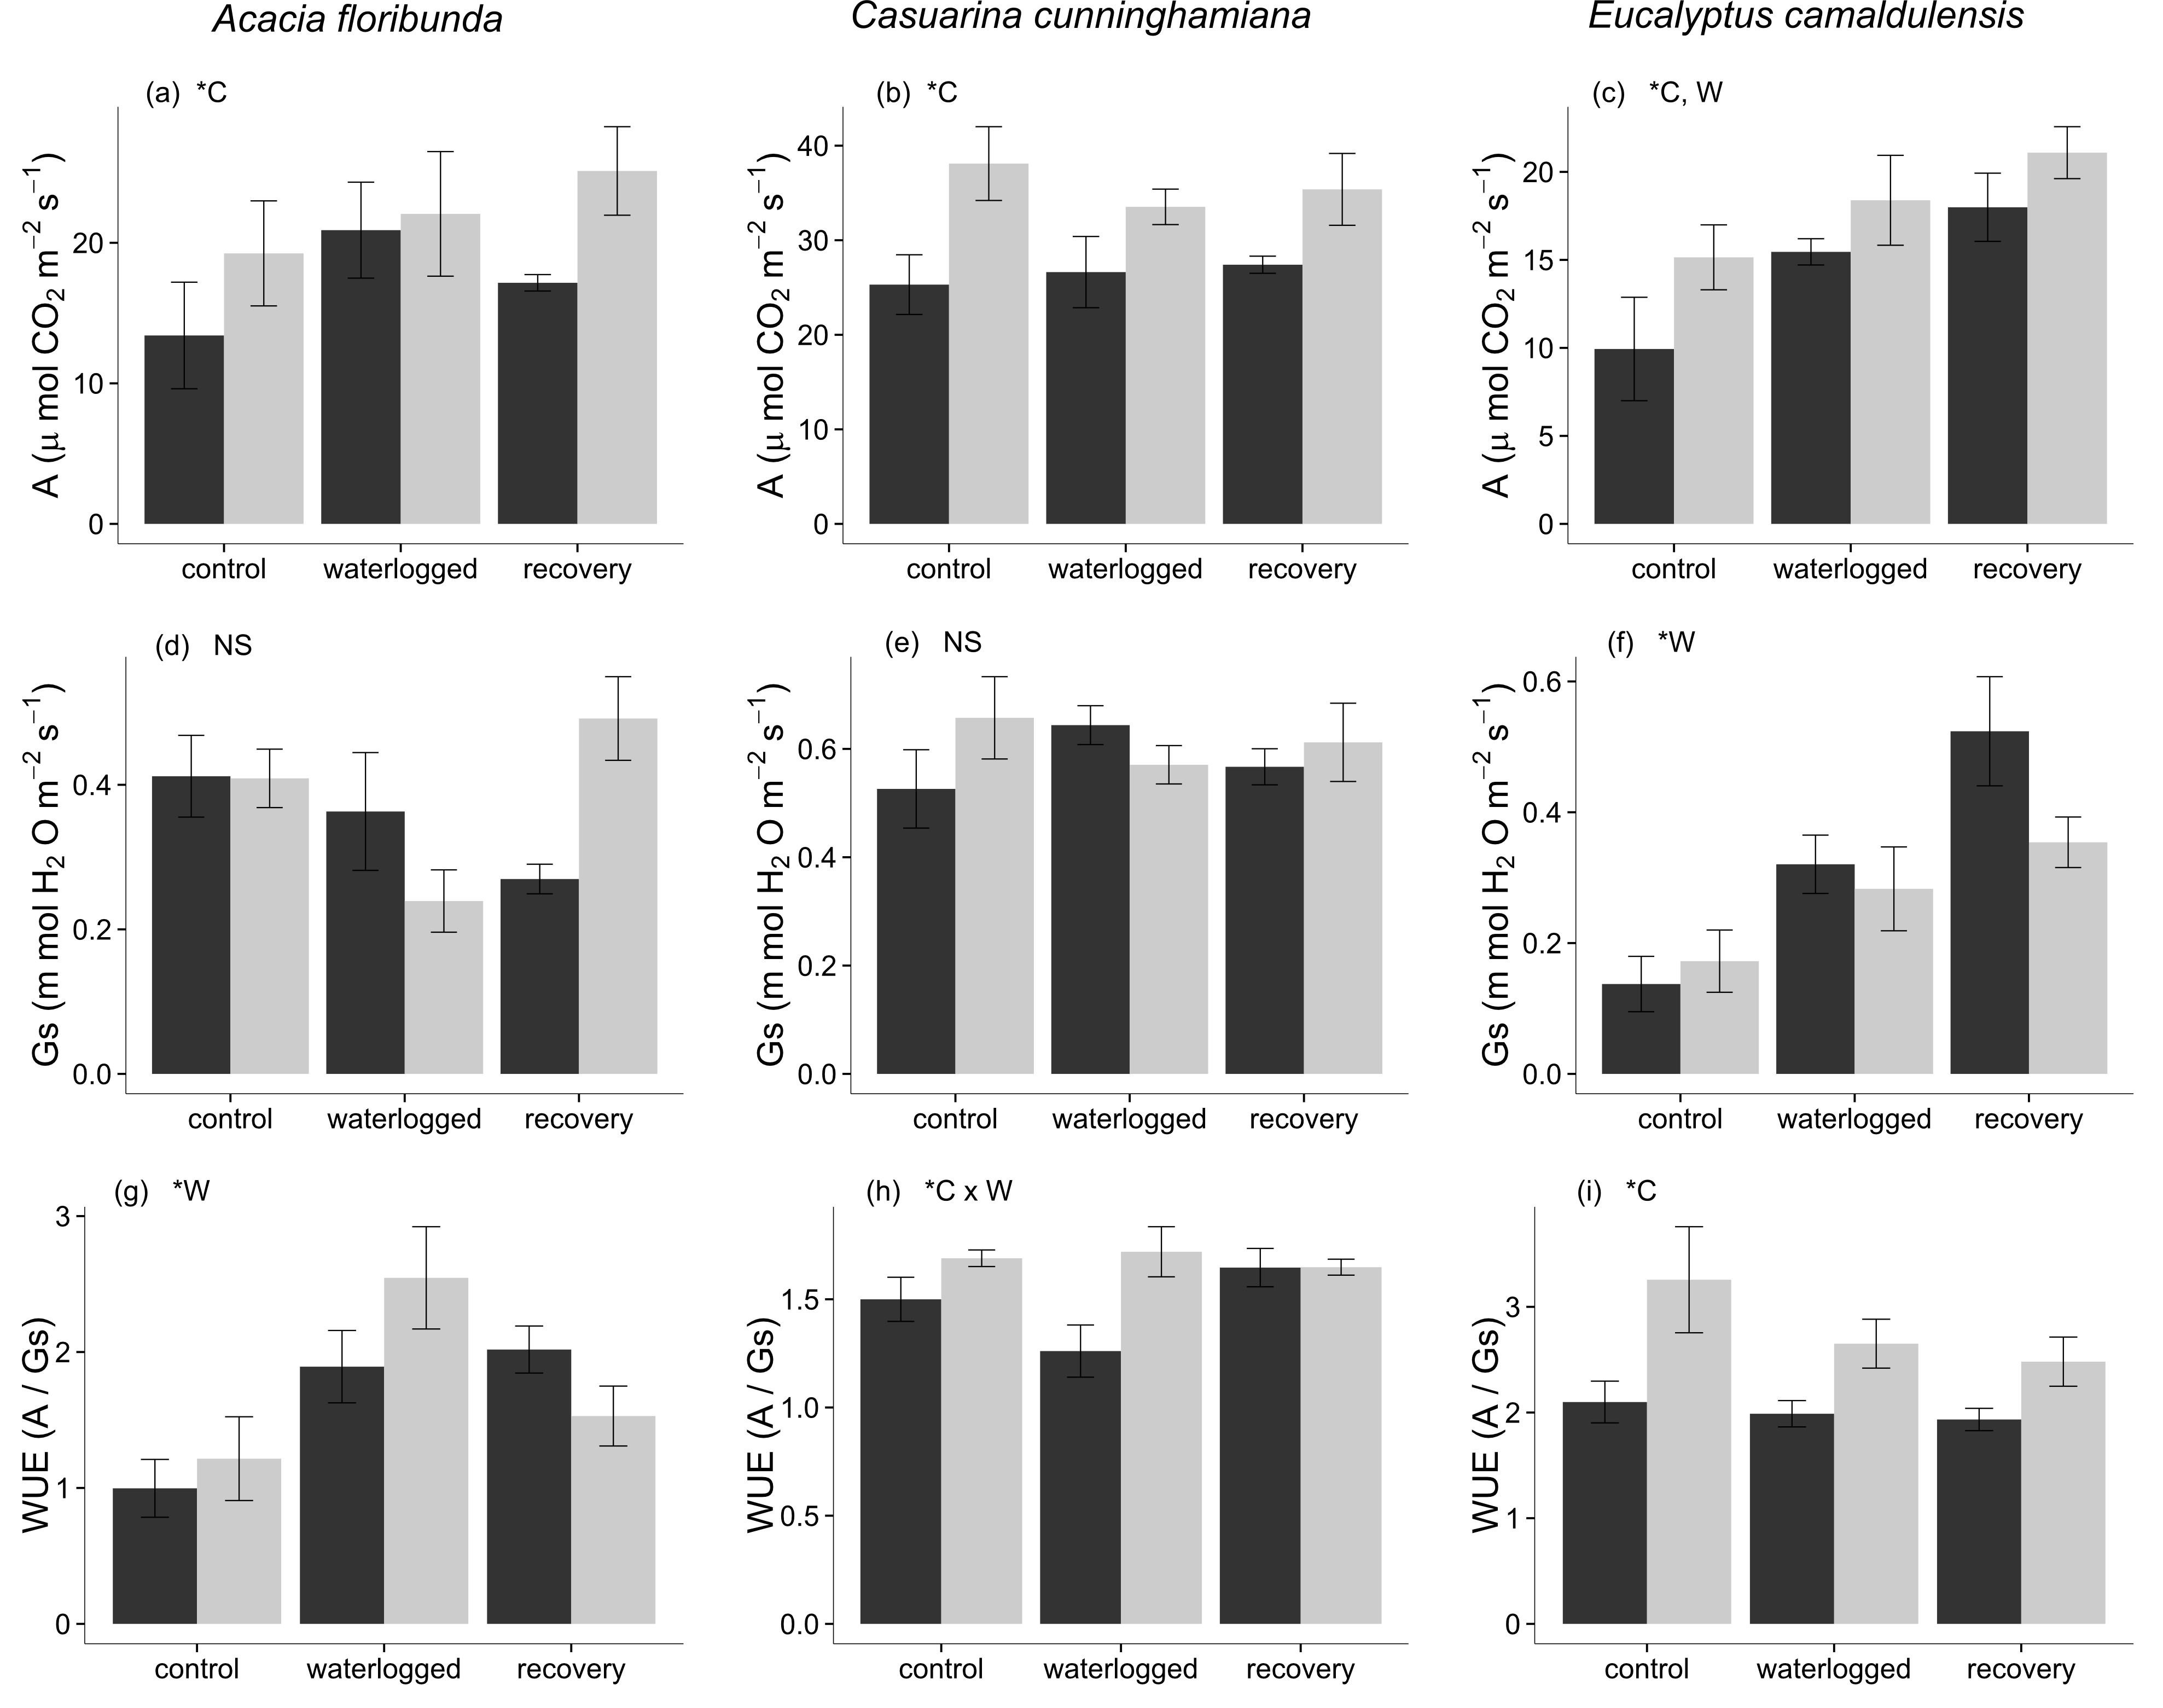
\includegraphics[width=\linewidth,keepaspectratio=true]{Ch5gasexchange2.png} % figures can be in pdf, png, jpeg or eps format
\caption[Gas exchange measurements under each combination of waterlogging and CO\textsubscript{2} level treatments.]{\small{Gas exchange measurements under each combination of waterlogging and CO\textsubscript{2} level treatments. Dark shaded columns represent measurements under ambient atmospheric CO\textsubscript{2} concentration (390 ppm), light shaded columns represent measurements under elevated atmospheric CO\textsubscript{2} concentration (550 ppm). Error bars represent the standardised mean error. \newline* letters denote statistical significance of differences between treatment combinations (NS = no significant difference, C = significant difference between CO\textsubscript{2} level treatments, W = significant difference between waterlogging treatments).}} %The caption in the square bracket is used for the table of figures. The caption in the curved brackets is the one that is printed as actual caption. 
\label{fig:Ch5_F1} % label for cross-referencing
\end{center}
\end{figure}

\subsection{Biomass production and allocation}
Waterlogging status and CO\textsubscript{2} level interacted strongly for one species: eCO\textsubscript{2} stimulation of all fractions of biomass production in \textit{C. cunninghamiana} was diminished following recovery from waterlogging. 

Total root biomass of plants recovering from waterlogging was lower than control plants for \textit{A. floribunda} (p = 0.028, Fig. \ref{fig:Ch5_F2}a). A significant interaction effect was identified for \textit{C. cunninghamiana} (p = 0.049): total root biomass was substantially increased under eCO\textsubscript{2} for control (p = 0.011) but not recovery plants (Fig. \ref{fig:Ch5_F2}b). Neither CO\textsubscript{2} level nor waterlogging had an effect on total root biomass for \textit{E. camaldulensis} (Fig. \ref{fig:Ch5_F2}c). 

Fine root biomass of \textit{A. floribunda} was lower in recovery plants than control plants (p = 0.005), with no CO\textsubscript{2} effect (Fig. \ref{fig:Ch5_F2}d). A marginally significant interaction effect was also present for \textit{C. cunninghamiana} fine root biomass (p = 0.076); post-hoc analysis confirmed that control but not recovery plants had significantly greater fine root biomass under eCO\textsubscript{2} (p = 0.008) (Fig. \ref{fig:Ch5_F2}e). Waterlogging stimulated fine root growth in \textit{E. camaldulensis} (p = 0.046) but CO\textsubscript{2} level had no effect (Fig. \ref{fig:Ch5_F2}f).

Neither CO\textsubscript{2} level nor waterlogging had any effect on shoot biomass for \textit{A. floribunda} (Fig. \ref{fig:Ch5_F2}g) or \textit{E. camaldulensis} (Fig. \ref{fig:Ch5_F2}i). As with total root biomass and fine root biomass, CO\textsubscript{2} level and waterlogging influenced \textit{C. cunninghamiana} biomass interactively (p = 0.009): shoot biomass was higher under eCO\textsubscript{2} for control (p = 0.015) but not recovery plants (Fig. \ref{fig:Ch5_F2}h).

Root mass fraction (RMF) was decreased by waterlogging for all species, but no significant CO\textsubscript{2} or interaction effects were found (Fig. \ref{fig:Ch5_F2}j-l). RMF of \textit{A. floribunda} was lower in waterlogged than control plants (p $<$ 0.0001), and lower in waterlogged than recovery plants (p $<$ 0.0001). RMF of \textit{A. floribunda} recovery plants was also lower than control plants (p = 0.016). RMF of both \textit{C. cunninghamiana} and \textit{E. camaldulensis} was lower in waterlogged than control plants (p $<$ 0.0001), and lower in waterlogged than recovery plants (p $<$ 0.0001), but there was no difference between recovery and control plants.

%%%% FIGURE 2
\begin{figure}[h!t]
\begin{center}
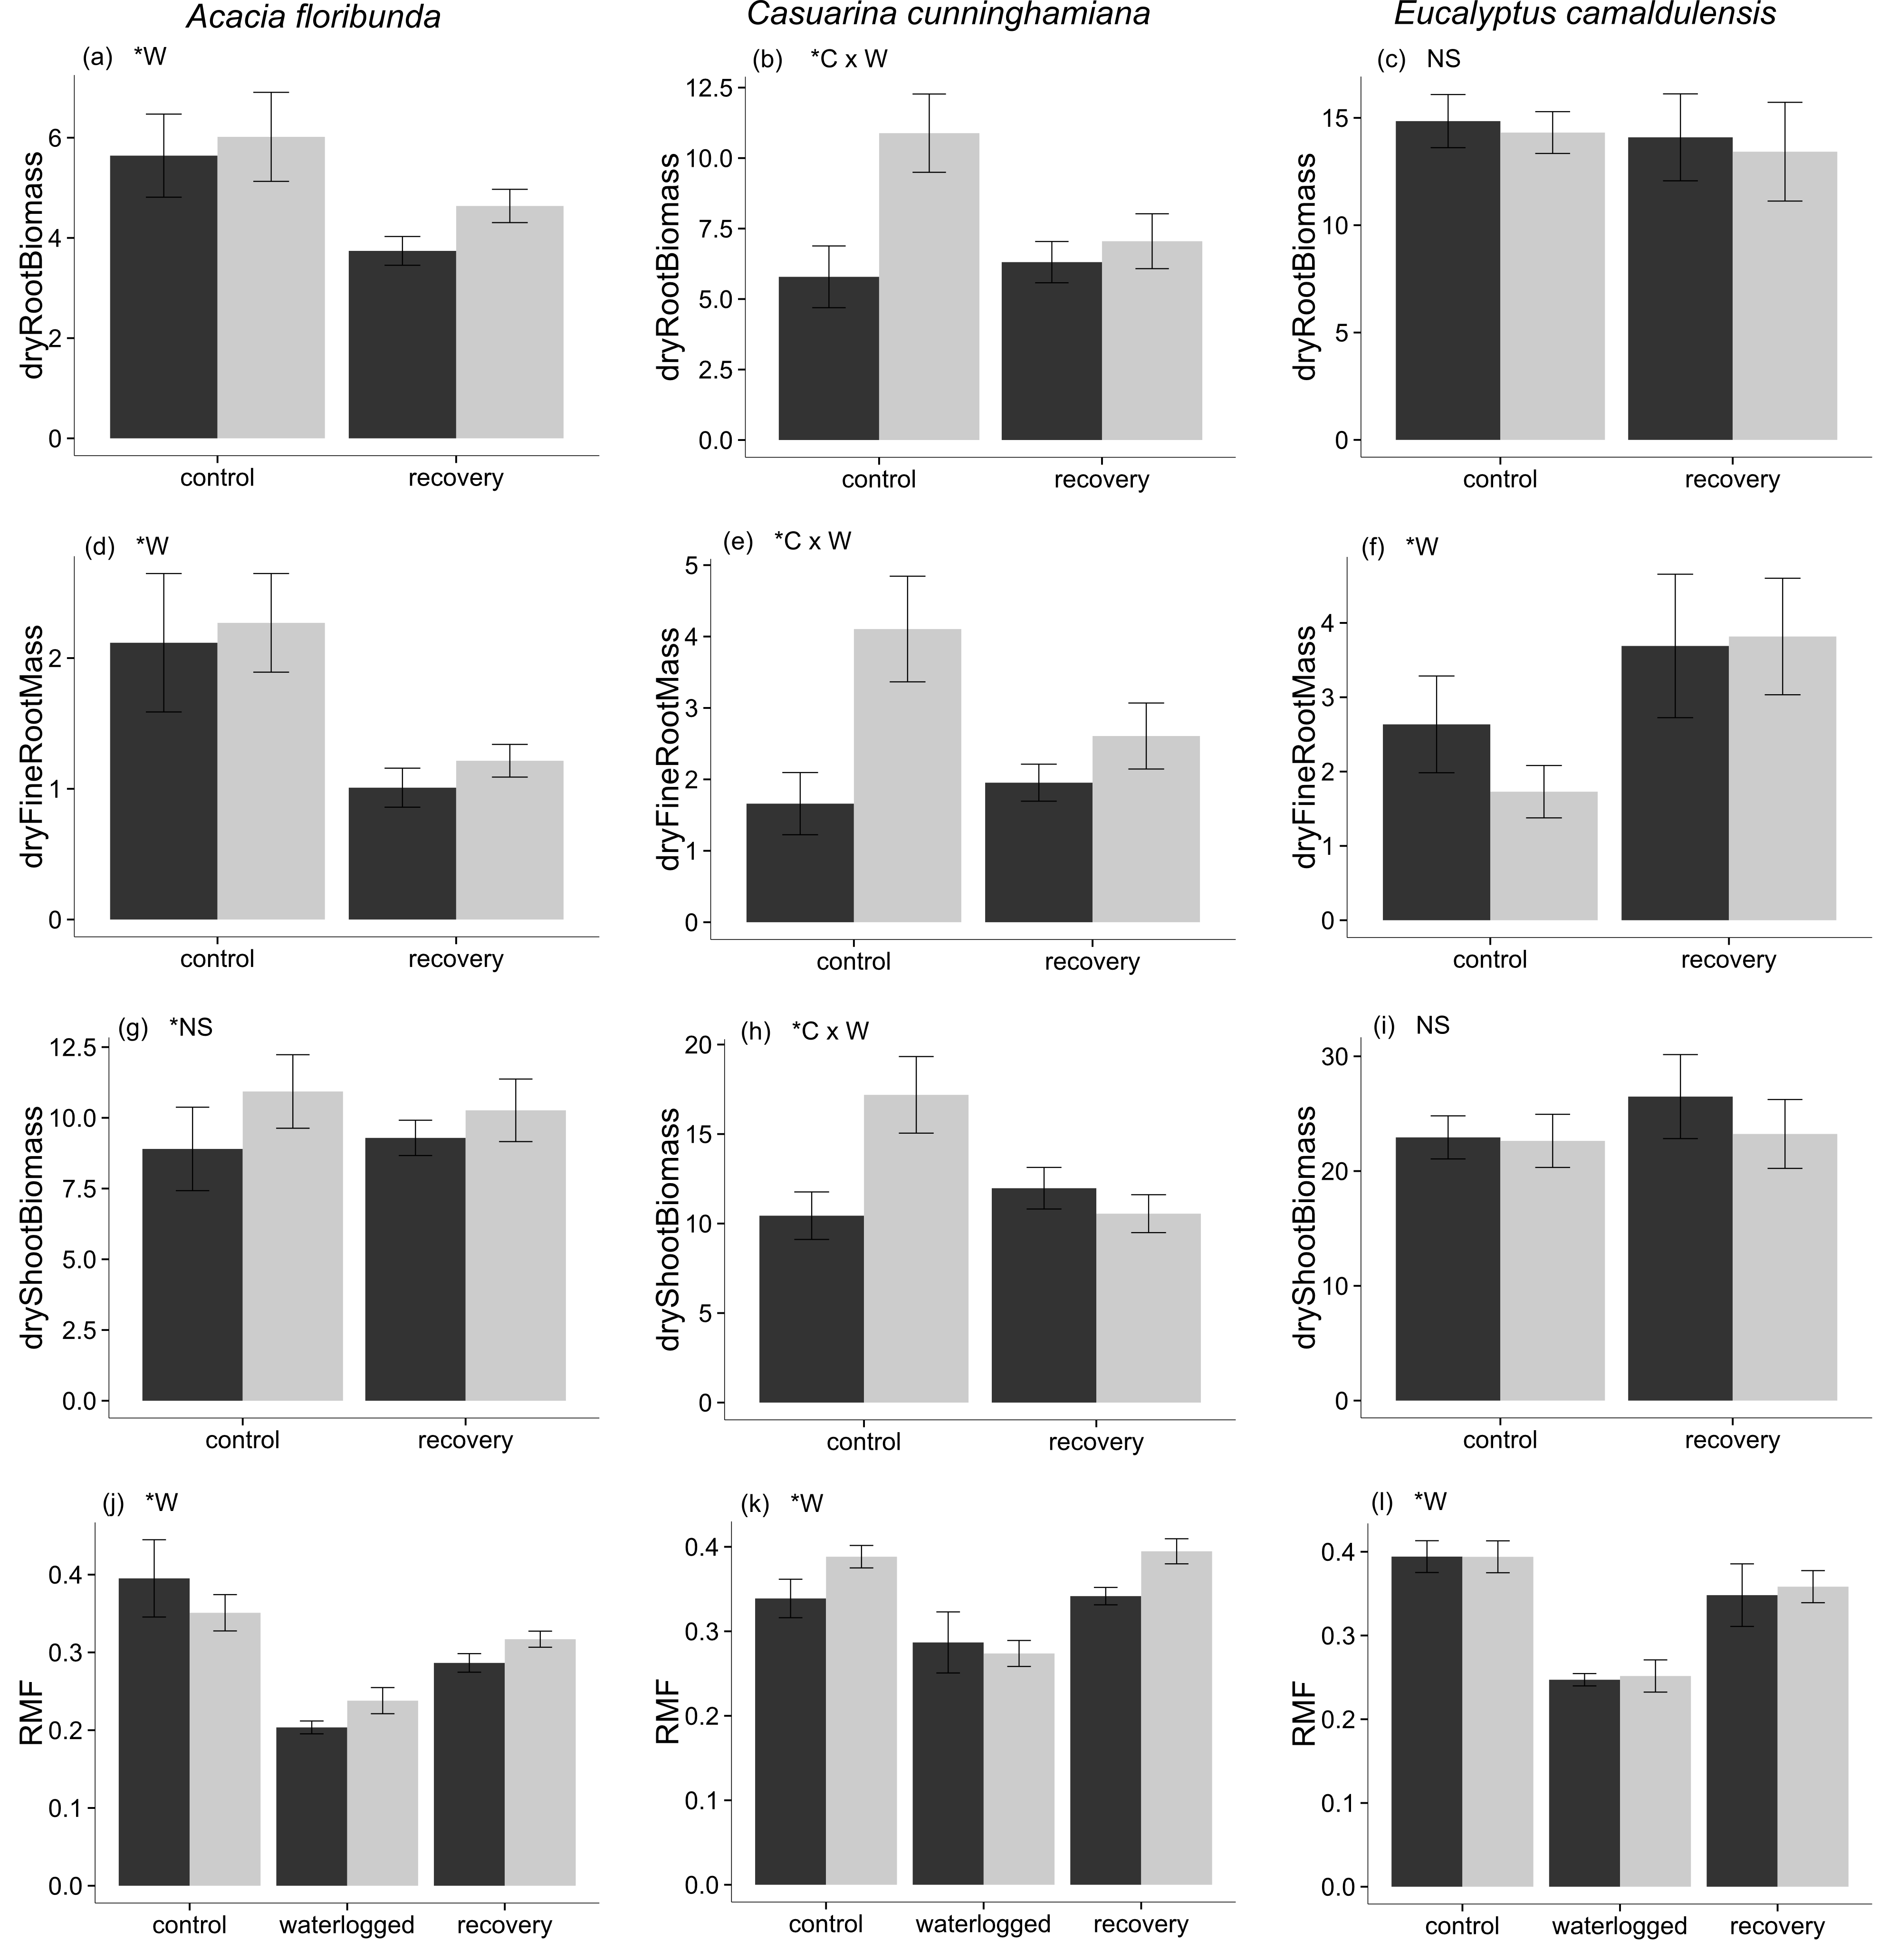
\includegraphics[width=\linewidth, keepaspectratio=true]{Ch5biomass2.png} % figures can be in pdf, png, jpeg or eps format
\caption[Biomass and root mass fraction (RMF) measurements under each combination of waterlogging and CO\textsubscript{2} level treatments.]{\small{Biomass and root mass fraction (RMF) measurements under each combination of waterlogging and CO\textsubscript{2} level treatments. Dark shaded columns represent measurements under ambient CO\textsubscript{2} concentration (390 ppm), light shaded columns represent measurements under elevated CO\textsubscript{2} concentration (550 ppm). Error bars represent the standardised meanerror. \newline* letters denote statistical significance of differences between treatment combinations (NS = no significant difference, C = significant difference between CO\textsubscript{2} level treatments, W = significant difference between waterlogging treatments).}} %The caption in the square bracket is used for the table of figures. The caption in the curved brackets is the one that is printed as actual caption. 
\label{fig:Ch5_F2} % label for cross-referencing
\end{center}
\end{figure}

\subsection{Functional traits}
We found no evidence to suggest that CO\textsubscript{2} mediates functional traits in response to waterlogging status.

Fine root dry matter content (fRDMC) was higher in waterlogged \textit{A. floribunda} than recovery plants (p = 0.027), but not different between control and recovery or control and waterlogged plants. A marginally significant interaction effect was also present for \textit{A. floribunda} (p = 0.067), but no differences were significant upon post-hoc analysis. Waterlogging status also affected \textit{E. camaldulensis} fRDMC (Fig. \ref{fig:Ch5_F3}b): control plants had higher fRDMC than waterlogged plants (p = 0.018), and recovery plants (p = 0.053) (marginally significant). eCO\textsubscript{2} was associated with significantly increased fRDMC in \textit{C. cunninghamiana} (p = 0.013, Fig. \ref{fig:Ch5_F3}c), but waterlogging status had no effect.

Waterlogged \textit{A. floribunda} had lower SLA than control (p = 0.001), and recovery plants (p $<$ 0.0001) (Fig. \ref{fig:Ch5_F3} d). Waterlogged \textit{E. camaldulensis} had higher SLA than control (p = 0.0013) and recovery plants (p = 0.0006) (Fig. \ref{fig:Ch5_F3}f). Waterlogging status had no effect on \textit{C. cunninghamiana} SLA (Fig. \ref{fig:Ch5_F3}e). CO\textsubscript{2} level had no effect on the SLA of any species. 

Stem density in \textit{C. cunninghamiana} was increased under elevated CO\textsubscript{2} (p = 0.0177) (Fig. \ref{fig:Ch5_F3}h). Stem density was lower in waterlogged \textit{C. cunninghamiana} than control (p = 0.0167) or recovery plants (0.050) Neither CO\textsubscript{2} nor waterlogging status had any effect on stem density of \textit{A. floribunda} (Fig. \ref{fig:Ch5_F3}g) or \textit{E. camaldulensis} (Fig. \ref{fig:Ch5_F3}i).

%%%% FIGURE 3
\begin{figure}[h!t]
\begin{center}
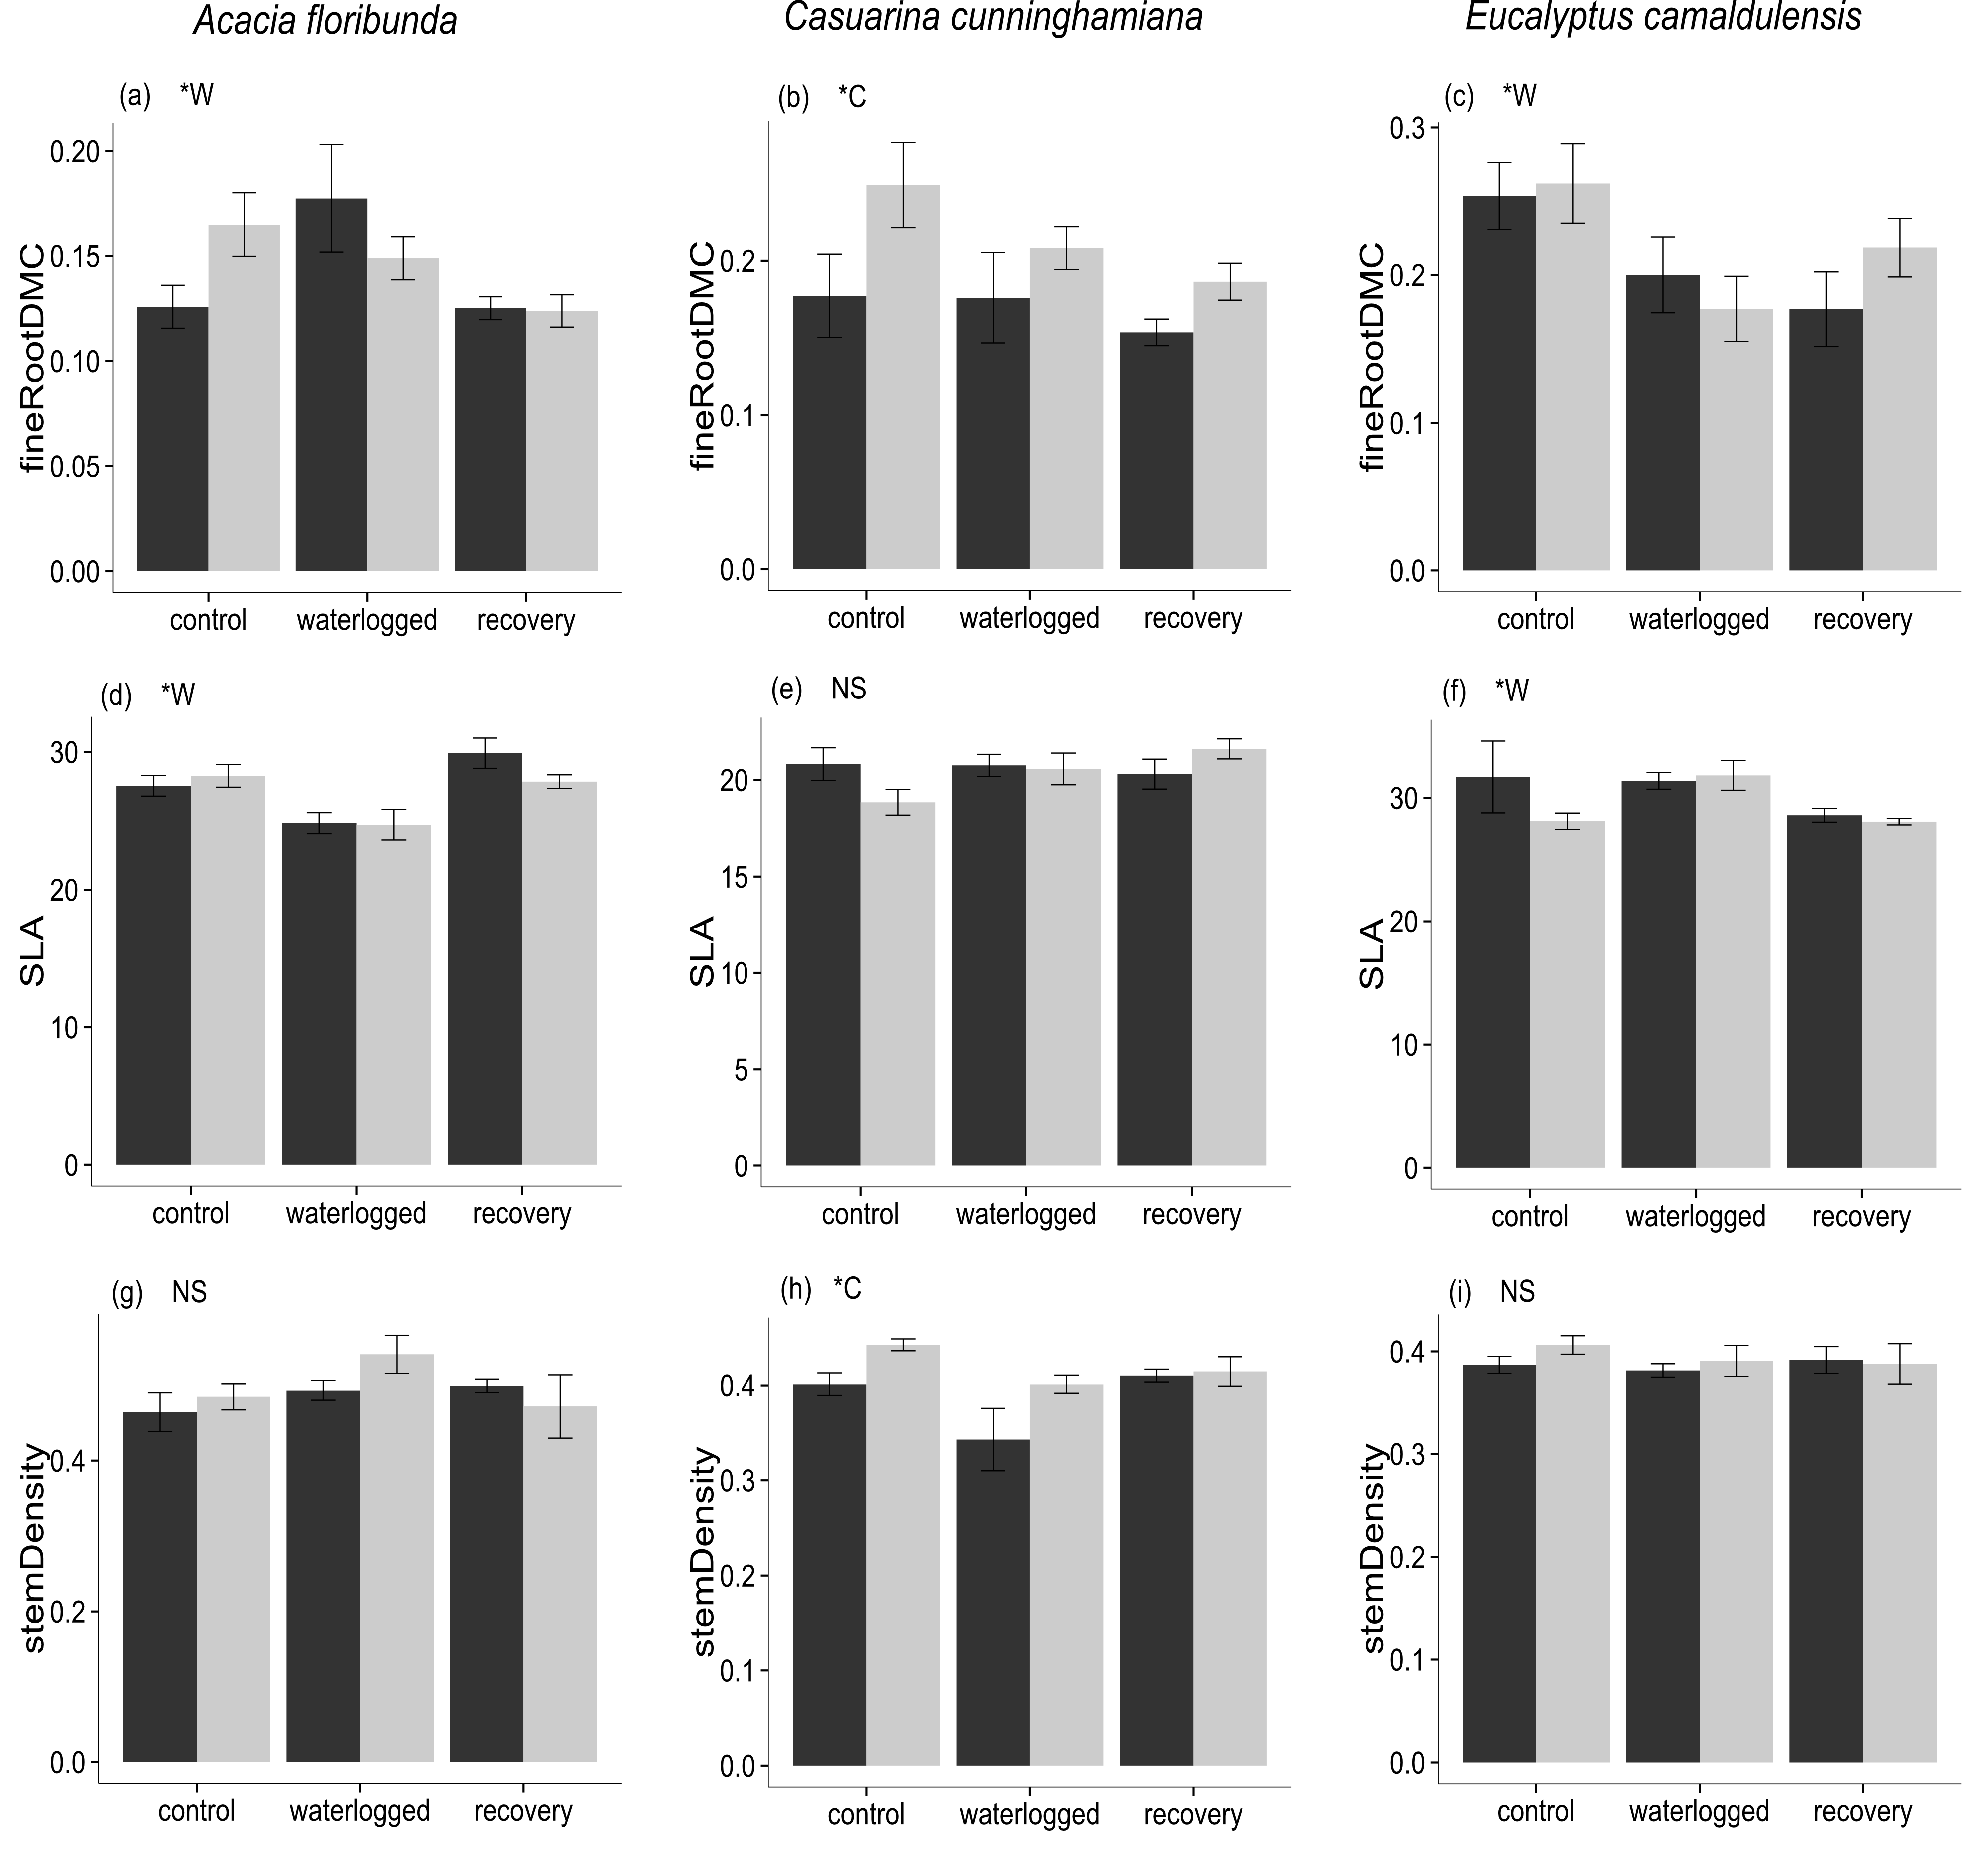
\includegraphics[width=\linewidth,keepaspectratio=true]{Ch5traits2.png} % figures can be in pdf, png, jpeg or eps format
\caption[Functional trait measurements under each combination of waterlogging and CO\textsubscript{2} level treatments.]{\small{Functional trait measurements under each combination of waterlogging and CO\textsubscript{2} level treatments. Dark shaded columns represent measurements under ambient CO\textsubscript{2} concentration (390 ppm), light shaded columns represent measurements under elevated CO\textsubscript{2} concentration (550 ppm). Error bars represent the standardised mean error. \newline* letters denote statistical significance of differences between treatment combinations (NS = no significant difference, C = significant difference between CO\textsubscript{2} level treatments, W = significant difference between waterlogging treatments).}} %The caption in the square bracket is used for the table of figures. The caption in the curved brackets is the one that is printed as actual caption. 
\label{fig:Ch5_F3} % label for cross-referencing
\end{center}
\end{figure}

\section{Discussion}
We found inconsistent effects of atmospheric CO\textsubscript{2} concentration and waterlogging status on growth, gas exchange and functional traits between species of riparian tree seedlings and no evidence for a consistent effect of elevated CO\textsubscript{2} in mediating plant responses to flooding. 

While photosynthesis is the primary means by which plants accumulate biomass, increases in leaf-level photosynthesis may not necessarily translate to biomass gains. Metabolically costly responses to waterlogging tolerance, such as anaerobic catabolism, detoxification of reactive oxygen species and metal ions, and morphological adaptations such as formation of adventitious roots may act as energetic sinks \citep{Colmer2009}. Relationships between photosynthetic rate and biomass responses to waterlogging and CO\textsubscript{2} level treatments in this study varied widely between species.

For the three species studied here, only for \textit{C. cunninghamiana} was an interactive effect of CO\textsubscript{2} concentration and waterlogging status found. Biomass of shoot, total root and fine root fractions was significantly higher under eCO\textsubscript{2} for control \textit{C. cunninghamiana} plants, but not for plants which were recovering from waterlogging, despite increased rates of CO\textsubscript{2} assimilation. No significant interaction effect on root mass fraction was found, but visual inspection of the data (Fig. \ref{fig:Ch5_F2}k) indicates that eCO\textsubscript{2} stimulation of RMF was present in control and recovering, but not waterlogged plants. Re-establishment of pre-waterlogging biomass allocation appears to have occurred despite no differences in total biomass. We found no evidence to support the hypothesis that eCO\textsubscript{2} facilitated biomass recovery by increasing the rate of fine root production in \textit{C. cunninghamiana} after waterlogging. Photosynthesis remained higher in recovering plants under eCO\textsubscript{2}, indicating that their ability to convert the extra photosynthate produced under eCO\textsubscript{2} into biomass was impaired by waterlogging. 

No increase in any biomass fraction was associated with increased photosynthetic rate under eCO\textsubscript{2} for either \textit{A. floribunda} or \textit{E. camaldulensis}. \textit{A. floribunda} underwent substantial root mortality in response to waterlogging, although the presence of spongy white aerenchymous adventitious roots indicated a degree of morphological adaptation to anoxia \citep{Evans2004}. Conversely, waterlogging stimulated fine root growth in \textit{E. camaldulensis}. A proliferation of fine aerenchymous roots both below and above the water line was observed in waterlogged and recovered plants, corresponding to increased fine root mass compared with control plants. The strong morphological response of \textit{E. camaldulensis} root systems combined with higher photosynthetic rate in recovering compared with control plants, and higher stomatal conductance in waterlogged plants than control or recovering plants, indicates that \textit{E. camaldulensis} responded favourably to waterlogging in this study. This growth response concurs with the results of previous studies \citep{Sena-Gomes1980, Marcar1993}, although see \citep{Kogawara2006}. No evidence was found to support the hypothesis that higher water use efficiency under eCO\textsubscript{2} might facilitate photosynthesis where waterlogging had caused stomatal closure. WUE was altered by waterlogging only in \textit{A. floribunda}, and by CO\textsubscript{2} level only in \textit{E. camaldulensis}. WUE was dependent on the combination of waterlogging status and CO\textsubscript{2} level in \textit{C. cunninghamiana}, being higher at eCO\textsubscript{2} than aCO\textsubscript{2} for waterlogged plants only. The lack of stomatal response to waterlogging indicates that higher WUE under eCO\textsubscript{2} is not the mechanism maintaining photosynthetic rate under waterlogging for C. cunninghamiana. 

Waterlogging and atmospheric CO\textsubscript{2} level also altered functional traits in a species-specific manner, but no interactive effects were found. Traits of \textit{A. floribunda} and \textit{E. camaldulensis} were affected by waterlogging status but not CO\textsubscript{2} level, whereas \textit{C. cunninghamiana} was affected by CO\textsubscript{2}. Decreased SLA and increased fine root dry matter content – a proxy for fine root tissue density \citep{Birouste2013} – in waterlogged \textit{A. floribunda} indicate a shift towards the slower growth – longer lifespan  end of their respective economic spectra \citep{Reich2014}, but this shift was not sustained following the refractory period. A corresponding pattern in water use efficiency corroborates this inference. Higher root dry matter content under waterlogging has been linked to the requirement for structural support of air spaces in aerenchymous root tissue \citep{Ryser2011}. Suberization of root hypodermal tissue often occurs under waterlogging as a means of reducing radial oxygen loss \citep{Visser2000, DeSimone2002} and may also increase root dry matter content. \textit{E. camaldulensis} responded in an opposite manner, with higher SLA under waterlogging, and lower root dry matter content under waterlogging and after the refractory period. This species appears to employ an opportunistic ‘fast growth’ ecological strategy in response to waterlogging, involving proliferation of lower density roots, and lower carbon investment in leaf tissue \citep{Wright2004, Reich2014}. We found no evidence for decreased SLA under eCO\textsubscript{2} as previously described \citep{Poorter2003a}. Previous studies report inconsistent effects of eCO\textsubscript{2} on fine root dry matter content in non-riparian species: eCO\textsubscript{2} had no effect on \textit{Liquidambar styraciflua} or \textit{Pinus strobus} fRDMC \citep{Bauer2001,Iversen2008}, caused a small decrease in \textit{Betula alleghaniensis} \citep{Bauer2001} and increased fRDMC in cotton \citep{Prior1994}. In this study, eCO\textsubscript{2} significantly increased fine root dry matter content in \textit{C. cunninghamiana} irrespective of waterlogging treatment.

Analysis of gas exchange, biomass accumulation and functional traits after a refractory period provided an opportunity to determine whether responses to waterlogging persisted or were transitory. We were unable to substantiate the hypothesis that eCO\textsubscript{2} would increase the rate of biomass recovery from waterlogging by increasing the rate of fine root turnover. \textit{C. cunninghamiana} was the only species for which eCO\textsubscript{2} altered biomass accumulation, and depression of biomass was observed following the refractory period irrespective of CO\textsubscript{2} level. Although we made no analysis of nodulation rates, nodulation of \textit{C. cunninghamiana} by the nitrogen fixing ascomycete \textit{Frankia} is known to be highest under well aerated soil conditions \citep{Dawson1989}. Reduced nitrogen uptake due to nodule mortality or impairment could account for the constrained biomass response to eCO\textsubscript{2} post-waterlogging \citep{Reich2006}. While eCO\textsubscript{2} did not mitigate growth reduction or mediate changes to functional traits under waterlogging for any species in this glasshouse study, we did observe reduced growth stimulation by eCO\textsubscript{2} in one species. This effect was strong, and evident across all measured biomass fractions. Differential responses to eCO\textsubscript{2} and waterlogging between species in the field could have important ecological consequences. \textit{C. cunninghamiana} is a highly effective agent of ‘biogeomorphic succession’ in fluvial landscape of south-eastern Australia – that is, it facilitates the creation and stabilisation of fluvial landforms \citep{Erskine2009}. Reduction of eCO\textsubscript{2} biomass stimulation by waterlogging could alter spatial patterns of landform stabilisation by \textit{C. cunninghamiana}. Infrequently waterlogged stands on channel banks might be favoured over stands growing on wetter in-channel features such as bars, benches and islands. Differential responses to combined waterlogging and eCO\textsubscript{2} between species – notably \textit{C. cunninghamiana} and \textit{A. floribunda}, which are frequently conspecific – may also result in compositional changes to riparian plant communities and associated changes in ecosystem functioning.

\section{Conclusion}
Waterlogging and atmospheric CO\textsubscript{2} concentration both have significant consequences for physiological processes, growth and functional characteristics of riparian tree seedlings. The relative importance of these environmental factors varies according to species, as do the specific effects of each on plants. This study adds to the small but growing body of literature describing the interactive effects of waterlogging and CO\textsubscript{2} concentration; notably, the outcome for \textit{C. cunninghamiana} concurs with that found for \textit{Taxodium distichum}, a flood tolerant colonist of alluvial riparian areas in the south eastern United States \citep{Megonigal2005}. Suppression of eCO\textsubscript{2} biomass stimulation in seedlings by waterlogging has the potential to alter demographics and structural dynamics in many Australian riparian communities especially where \textit{C. cunninghamiana} is a keystone species \citep{Woolfrey2001}.

\section*{Acknowledgements}
We would like to thank Urvashi Lallu, Claire Laws, Muhammad Masood, Daniel Sloane, Samiya Tabassum for their help in the glasshouse, and Anthony Manea, Brian Atwell and Melanie Zeppel for providing advice on study design and implementation.

\clearpage

%%%%% REFERENCES % this is in a new chapter due to the memoir format
\renewcommand\bibname{{References}} 
\begin{small}
\bibliographystyle{apalike}
\bibliography{library.bib}
\end{small}



\clearpage

%%%%%%%%%%%%%%%%%%%%%%%%%%%%%%%%%
% CHAPTER 6
%
%%%%%%%%%%%%%%%%%%%%%%%%%%%%%%%%%%%%%%%%%%%%%%%%%%%%%%%%%%%%%%%%%%%%%%
% Tina Dissertation
% December 2013, modified to Template June 2015
%%%%%%%%%%%%%%%%%%%%%%%%%%%%%%%%%%%%%%%%%%%%%%%%%%%%%%%%%%%%%%%%%%%%%%
% Documentclass Memoir 
% check memman.pdf for help and information
%%%%%%%%%%%%%%%%%%%%%%%%%%%%%%%%%%%%%%%%%%%%%%%%%%%%%%%%%%%%%%%%%%%%%%
\documentclass[12pt,a4paper]{memoir} 
\usepackage{graphicx}
%\usepackage[utf8]{inputenc} % set input encoding to utf8
\usepackage{array} % for tables 
\usepackage{multirow} % for tables 
\usepackage{multicol} % for tables
\usepackage{tabularx} % for tables
\usepackage{booktabs}
\usepackage{cite}
\usepackage{tabularx}
\usepackage[round]{natbib}
\usepackage{threeparttable}
\DisemulatePackage{setspace}
\usepackage{setspace}
\usepackage{longtable}
\usepackage{tabu}
\usepackage{pdflscape}
\usepackage{caption}
 %\useunder{\uline}{\ul}{}

% defines new column type
\newcolumntype{Z}{>{\raggedright\arraybackslash}X}

% add a little vertical padding to cramped tables
\setlength{\extrarowheight}{2pt}


%%%%%%%%%%%%%%%%%%%%%%%%%%%%%%%%%%%%%%%%%%%%%%%%%%%%%%%%%%%%%%%%%%
%%% Examples of Memoir customization
%%% enable, disable or adjust these as desired

%%% PAGE DIMENSIONS
% a4paper is by default 210mm wide and 279 mm wide

% default document in memoir is twoside (recto-verso) and openright (new chapter begins on recto page)

% size of the text area
\settrims{0pt}{0pt}
\settypeblocksize{230mm}{147mm}{*}
\setlength{\spinemargin}{27mm}
\setlength{\foremargin}{36mm}
%\setulmargins{35mm}{45mm}{*}
%\setlength{\marginparwidth}{0mm}
%\setlength{\marginparsep}{0mm}
%\setlength{\textwidth}{140mm}
%\settrimmedsize{0.9\stockheight}{0.9\stockwidth}{*}
%\setlength{\trimtop}{0pt}
%\setlength{\trimedge}{0pt}
%\addtolength{\trimedge}{-\paperwidth}
%\settypeblocksize{*}{\lxvchars}{1.618} % we want to the text block to have golden proportionals
\setulmargins{*}{*}{1.618} % 50pt upper margins
%\setlrmargins{*}{*}{1.3}
\setlrmargins{*}{*}{1} % golden ratio again for left/right margins
\setheaderspaces{*}{*}{1.618}
\checkandfixthelayout % to make sure that the layout parameters make sense

%\addtolength{\textwidth}{0cm}
%\addtolength{\textheight}{1.5cm}
%\addtolength{\textwidth}{-2cm}
%\addtolength{\textheight}{+0.5cm}

%%% \maketitle CUSTOMISATION
% For more than trivial changes, you may as well do it yourself in a titlepage environment
%\pretitle{\begin{center}\sffamily\Huge\MakeUppercase}
%\posttitle{\par\end{center}\vskip 0.5em}

%%% ToC (table of contents) APPEARANCE
\maxtocdepth{subsection} % include subsections
%\renewcommand{\cftchapterpagefont}{}
%\renewcommand{\cftchapterfont}{}     % no bold!

%%% HEADERS & FOOTERS
\pagestyle{Ruled} % try also: empty , plain , headings , ruled , Ruled , companion

%%% CHAPTERS
\chapterstyle{southall} % try also: default , section , hangnum , companion , article, demo

\renewcommand{\chaptitlefont}{\LARGE\sffamily\raggedright} % set sans serif chapter title font
\renewcommand{\chapnumfont}{\LARGE\sffamily\raggedright} % set sans serif chapter number font

%%% TABLES
\newcolumntype{C}[1]{>{\centering}m{#1}} % defines the default layout of the tables (C=centerling, L=left)
\newcolumntype{L}[1]{>{\centering}m{#1}}

%%% SECTIONS
%\hangsecnum % hang the section numbers into the margin to match \chapterstyle{hangnum}
\maxsecnumdepth{section} % number subsections

\setsecheadstyle{\Large\sffamily\raggedright} % set sans serif section font
\setsubsecheadstyle{\large\sffamily\raggedright} % set sans serif subsection font

%%% Abstract
\setlength{\absleftindent}{0mm}
\setlength{\absrightindent}{0mm}

\renewcommand{\absnamepos}{center}
\setlength{\abstitleskip}{+0cm}

%% END Memoir customization
%%%%%%%%%%%%%%%%%%%%%%%%%%%%%%%%%%%%%%%%%%%%%%%%%%%%%%%%%%%%%%%%%%%%%%%%%%%%%%%%%%%%%%%%%%%%%%%%%%%%%%%%%%%%%%%%%%%%%%%%%%%%%%%%%%%%%%%%%%%%%
%%% BEGIN DOCUMENT

\begin{document}
\doublespacing

\chapter[Discussion]{Discussion}
\newpage

\noindent{In this thesis I explored how natural and altered environmental conditions shape the ecology of riparian plant communities. In this final chapter I aim to summarise the contribution of my thesis to the greater body of riparian plant ecology and river restoration research, outline outstanding questions raised by my work, and present some possible avenues for future work.}

\section{Summary of findings}
In Chapter 2, I asked the following research questions: (1) does wood density increase with increasing frequency and magnitude of flood disturbance? (2) does wood density increase with increasing unpredictability of water availability in the riparian zone? (3) does dispersion of wood density peak at intermediate levels of hydrological disturbance? I found evidence for an affirmative answer to all three questions. Community mean wood density was strong correlated with metrics of frequency and magnitude of flood disturbance, as well as variability of water availability in the riparian zone, and dispersion of wood density indeed peaked at intermediate levels of hydrological disturbance and variability.

In Chapter 3, I asked: (1) Is functional trait diversity related to the frequency and magnitude of flooding disturbance? (2) Is functional trait diversity related to variability in seasonal water availability within the riparian zone? I found strong associations between functional trait diversity and metrics describing frequency and magnitude of flooding disturbance and variability in seasonal water availability within the riparian zone.

In Chapter 4, I investigated relationships between environmental variables and species richness, functional trait diversity, and exotic abundance, with a focus on the role of environmental heterogeneity and modification of river flows and landscapes by human activity. I asked: (1a) do species richness and functional diversity increase and abundance of exotic species decrease monotonically with increasing hydrological heterogeneity? (1b) do species richness, functional diversity and abundance of exotic species show unimodal relationships with hydrological heterogeneity? (2) do species richness and functional diversity decrease and abundance of exotic species increase along gradients of increasing flow modification and catchment land-use intensity? With respect to (1a), patterns of species richness and exotic abundance were opposite to expectation, and findings were inconclusive for functional trait diversity. Our findings were also inconclusive with respect to (1b), with limited evidence that functional diversity is unimodally related to hydrological heterogeneity. Relationships between species richness and exotic abundance with metrics of flow modification opposed our expectation under (2), and while production land use was associated with higher exotic abundance, no effect of land use on species richness was found. I found weak evidence supporting flow modification as a control on functional diversity, and no evidence for an effect of catchment land-use intensity.

In Chapter 5, I tested for interactive effects between eCO\textsubscript{2} and waterlogging on gas exchange, biomass accumulation and allocation, and functional traits in riparian tree seedlings. I found no interactive effects on \textit{Acacia floribunda} or \textit{Eucalyptus camaldulensis}, but strong interactive effects on \textit{Casuarina cunninghamiana}.

\section{Biogeographic context}
The riparian plant communities described here were located primarily along coastally drained rivers in partly constrained valley settings, spanning the temperate south-east and subtropical eastern Australia. A map of the field sites surveyed in Chapters 2-4 is shown in Appendix 3. Although no systematic review has summarised ecological knowledge of Australian riparian plant communities, more research attention appears to have been focused on semi-arid, inland-draining systems such as the Murray Darling Basin, or larger tropical rivers, than on these smaller coastal systems.

Much of the canonical riparian plant ecology literature focuses on alluvial river systems in Europe and North America \citep{Nilsson1989, Naiman1997, Tabacchi1998, Naiman2005, Corenblit2007}. Flow regimes in south-eastern Australia diverge considerably from this canon: the seasonal regularity which characterises nival European and North American rivers is often absent. In Australia, substantial year-by-year variability is evident and Australian rivers are known for having some of the highest coefficients of flow variability in the world \citep{Peel2004, Rustomji2009}. South-eastern Australian riparian plants exhibit characteristic species-level responses to seasonality, although there is no general coordination of growth and reproductive phenologies as in the Northern Hemisphere \citep{Ford1979}. As such, Australian riparian plant communities are likely to be adapted to different environmental controls. In common with North American systems, however, the signature of rapid landscape modification has been etched deeply into fluvial landscapes. Many rivers have undergone irreversible transitions in physical and ecological condition following European settlement \citep{Knopf1988, Fleischner1994, Wasson1994, Brierley1999}, and the mid-20th century saw the rise of extensive flow impoundment schemes in both continents \citep{Lloyd2004, Graf2006}.

This body of work therefore contributes fresh perspective to the global literature, from species pools subject to a different evolutionary history and operating under different environmental conditions to the most commonly described riparian ecosystems.

\section{Ecological responses of riparian plant communities to hydrology}
The relationship between environmental heterogeneity and biodiversity has been a key focus of ecologists since the early 1960’s \citep{MacArthur1961, Stein2014}. Riparian landscapes provide particularly useful model systems for exploring hypotheses about environmental heterogeneity due to strong control of biotic assemblages by hydrology. In tandem with disturbance, hydrologically-driven environmental heterogeneity has taken a central role in our conceptualisation of how riparian ecosystems function \citep{Poff1997, Naiman2005}.

Chapters 2, 3 and 4 tested hypotheses derived from this paradigm. Broadly, this work confirms the importance of hydrological heterogeneity and fluvial disturbance in shaping riparian plant assemblages. The specific contribution of these chapters to the riparian literature lies in the mechanistic, functional trait-based approach used. Through the lens of functional traits, I have begun to address questions about how flow regime influences ecological strategies of riparian plants at the community level, and how the functional organisation of communities varies along hydrological gradients.

In Chapter 2, I found that wood density, a functional trait associated with resistance to mechanical disturbance and drought tolerance \citep{Chave2009, Niklas2010}, varied strongly in response to patterns of hydrology. Community mean values of wood density increased with the intensity of fluvial disturbance and flow heterogeneity; communities which experienced more variable flow conditions were shifted towards the ‘slow’, conservative end of the spectrum of resource-economic ecological strategies \citep{Reich2014a}. Wood density in turn influences wood decomposition rates \citep{Mori2013} which has implications for ecosystem nutrient cycling and energetic fluxes in riparian ecosystems \citep{Harmon1986}, as well as for the residence time of geomorphically active large woody debris in river systems {\citep{Gurnell2002, Cadol2010}. I also found a humped relationship between community-weighted variance in wood density and the same combined gradient of disturbance and hydrological heterogeneity, lending evidence to general hypotheses (from outside of the riparian literature) that intermediate levels of disturbance should promote divergence in disturbance-response strategies \citep{Grime2006, Sonnier2010}. Given the substantial cost to plants incurred in setting down dense woody tissue \citep{Falster2006}, these findings demonstrate that some of the key trade-offs negotiated by plants in riparian communities are made in response to fluvial disturbance and hydrological heterogeneity.
 
Plant life forms and qualitatively derived functional groups have been used for some time to describe functional organisation in riparian plant communities \citep{Brinson1993, Stromberg2010, Stromberg2013}. In Chapters 3 \& 4 I derived quantitative, continuous indices of functional diversity from vegetation survey and data for a range of functional traits with the intent of capturing key axes of variation in riparian plant ecological strategy. Using functional traits as descriptors of ecological strategy provides generality across systems \citep{Lavorel2002, Suding2008} for example by allowing comparison of communities with dissimilar assemblages, and negates any requirement for expert knowledge to assign species to qualitative functional groups. These indices of functional diversity also facilitate the use of quantitative modelling methods \citep{Mason2013}, and allow more solid inferences to be made about how individual components of flow regime influence community assembly and ecosystem processes than are possible using taxonomic metrics of diversity \citep{Tilman1997, Diaz1998}.

Patterns of variation in functional dispersion measured in natural landscapes of coastal south-eastern Australia (described in Chapter 3) showed strong positive relationships with metrics describing hydrological heterogeneity. While I did not systematically describe variation in species richness along hydrological gradients, species richness (but not the number of species used in the functional dispersion analysis) was significantly positively correlated with functional dispersion. I was able to generate a multiple regression model which explained 80 \% of the total variation in functional dispersion using three hydrological metrics. Partitioning of variance between this model and optimal models generated using climatic and soil variables, showed that a substantial proportion of variance explained by hydrology was not co-explained by climate or soil, further demonstrating the dominance of fluvial disturbance and flow variability in shaping the functional structure of these plant communities.

Riparian plant communities in south-eastern Queensland (described in Chapter 4) showed somewhat different responses to hydrology. Several additional environmental variables were taken into account to quantify the degree of anthropogenic modification both to the surrounding catchment and to the flow regime itself. In this study, I found functional richness and functional divergence (as measured by abundance-standardised functional dispersion) were associated with only a limited subset of metrics describing hydrological heterogeneity, and variance partitioning of models showed that relatively little variation in either functional richness or divergence was explained by hydrology when climate and soil properties were taken into account. Flow modification did explain some variation in metrics of functional diversity, but again, not independently. Contrary to our hypotheses, and to patterns commonly described in Northern hydroecological systems ({e.g. \citet{Naiman1997}), species richness declined as flow regimes became more heterogeneous. The observation that species richness and metrics of functional diversity showed opposite relationships with the same hydrological variables allowed us to determine that communities living under hydrologically heterogeneous conditions were maintaining functional diversity with a reduced species pool. 

\subsection{Outstanding questions about the role of hydrological heterogeneity in structuring communities}
Although hydrological conditions were associated with functional trait diversity in both regions analysed here, the relative importance of hydrological heterogeneity \textit{per se} differed. Some of the major outstanding questions in this thesis are why this might have been so, and which aspects of the findings can be generalised or extrapolated to systems in other regions within Australia and across the globe?

It is possible that Australian plant communities in fact have unique relationships with flow heterogeneity, given Australia's title of 'the planet’s most hydrologically variable continent' \citep{Peel2004, Rustomji2009}. A larger comparative study of factors shaping the functional ecology of riparian plant communities would be an essential step towards finding generalities in flow heterogeneity-diversity relationships, and would also provide further opportunity to investigate discontinuities in trends. Riparian researchers are becoming more interested in functional ecology, and it is possible that we will see global syntheses being made over the next decade. Research in regions underrepresented in the riparian ecology literature, such as the tropics and the developing world, would be of particular value in this endeavour.

Absent an exhaustive global comparative synthesis, comparing the specific findings of Chapter 3 and Chapter 4 reveals a possible explanation for their differences. While functional diversity of communities described in Chapter 3 scaled monotonically with most metrics of flow variability, and was positively associated with species richness, functional diversity of communities in south-east Queensland (Chapter 4) was significantly associated with only a small set of metrics describing flow variability (e.g. interannual variability in baseflow index, constancy of monthly maximum flows) and in those cases, relationships were better described by quadratic models. As noted previously, species richness showed inverted relationships with these metrics. To properly compare the results of these two chapters, a methodological issue must first be addressed: functional dispersion (FDis), \textit{sensu} \citet{Laliberte2010}, was used in Chapter 3, while standardised effect size FDis (FDis.SES), \textit{sensu} \citet{Mason2013}, was used in Chapter 4 as a measure of functional divergence. With the exception of a few outliers, FDis was tightly positively correlated with FDis.SES for the south-east Queensland dataset (Pearson's r = 0.75, p = 0.00000002). With respect to species richness, this confirms that standardising FDis for abundance was not responsible for inverting the species richness – functional diversity relationship.

In our discussion of Chapter 4, I noted that rhythmicity in temporal patterns of energy and resource availability and environmental heterogeneity may both act as controls on riparian plant diversity. I cited recent work showing that rhythmic seasonal flow activity fosters greater diversity in birds and fishes and greater net primary production in plant communities \citep{Jardine2015}, and that energy (and resource) availability may be more important than environmental heterogeneity in determining patterns of diversity \citep{Lundholm2009}. Thus differences between the findings of Chapters 3 and 4 could be explained by differences in the influence of these two factors. For this conceptual model to be useful, we need to describe some key components of its structure. Firstly, is it flow rhythmicity \textit{per se} which is important, or simply total energy availability, which happens to be maximised in rhythmic systems? If the former, can flows be both heterogeneous and rhythmic, or are the two factors inherently opposite? For example, can a river with high interannual variability in its baseflow index also experience highly regular summer flood flows? Perhaps cases at extreme ends of each spectrum are less interesting than those at intermediate levels of heterogeneity and energy availability / rhythmicity.
 
Perhaps a better way of conceptualising environmental control over diversity might be as a three dimensional relationship, where heterogeneity and energy availability (or flow rhythmicity) are incompletely orthogonal to each other. The curves presented in this thesis would then be two dimensional slices of a three dimensional volume. A challenge for future research in this field is therefore to explicitly include energy availability or flow rhythmicity in hypotheses about flow responses of plant communities, and to attempt to characterise how communities respond to both factors simultaneously.

\section{Responses of riparian plant communities to anthropogenic environmental change}
My interest in the functional ecology of riparian plant communities was initially motivated by the need for new approaches and perspectives towards conserving, rehabilitating and managing riparian landscapes in south-eastern Australia. The 20th century has seen unprecedented change in riverine ecosystems and these changes are likely to intensify over the current century \citep{Nilsson2000, Hennessy2008}. Compared with Europe and North America, applied river rehabilitation in Australia is somewhat hampered by a lack of basic ecological knowledge \citep{Brooks2007}. Thus one of the main aims of this thesis was to inform management with new information about riparian ecology in both natural and modified landscapes.

\subsection{How might riparian plant communities respond to climate change?}
Climate change is predicted to have global impacts on ecosystems in the 21st century \citep{IPCC2014}. Riparian ecosystems are likely to be particularly vulnerable due to their high exposure and sensitivity to changes in climate, in combination with pressures associated with extraction of provisioning ecosystem services by humans \citep{Capon2013}. Elevated concentrations of carbon dioxide (eCO\textsubscript{2}) represent the most direct and obvious change to the atmosphere. The potential influence of eCO\textsubscript{2} on plants and plant communities has been the topic of intensive research over the last two decades. To date, however, the implications for conservation management under high CO\textsubscript{2} regime are highly species and system specific, and are likely to be contingent on a slew of other environmental factors \citep{Poorter2003a, Norby2011, Poorter2011, Reich2014}. Basic research on the ecological effects of eCO\textsubscript{2} is needed for individual systems, and each piece of experimental work contributes to the greater outlook.

Of the three anthropogenic alterations investigated in this thesis, I suggest that elevated atmospheric CO\textsubscript{2} (eCO\textsubscript{2}) may have the smallest effect. I showed in Chapter 5 that eCO\textsubscript{2} significantly stimulated growth in only one of three riparian tree seedlings, and this effect was completely negated by inundation. Inundation itself had strong effects on gas exchange, growth and functional traits in all three species. Differential responses between species to combined waterlogging and eCO\textsubscript{2} may have flow-on effects to demographics, competition, and ultimately, community composition.
 
Chapter 5 contributes to what is currently a very small set of publications investigating the potential for interactive effects between future atmospheric concentrations of CO\textsubscript{2} and inundation or waterlogging events on terrestrial plants \citep{Megonigal2005, Shimono2012, Arenque2014}. I included an analysis of functional trait responses, as well as including a recovery phase in the experiment, neither of which have been previously attempted to our knowledge. Fruitful avenues for future work include study of more species, serial waterlogging treatments to better understand how eCO\textsubscript{2} influences on waterlogging recovery, analysis of leaf nutrient concentrations to determine the role of nutrient limitation in suppressing growth stimulation by eCO\textsubscript{2} \citep{Reich2014}, and mesocosm experiments to investigate the implications of eCO\textsubscript{2} – waterlogging interactions for competition.

Greater hydrological variability and intensity of extreme weather events characterise models of high CO\textsubscript{2} climates \citep{Hennessy2008, stocker2013climate}. Our research demonstrates that riparian plant communities vary substantially in their taxonomic and functional composition over gradients of hydrological heterogeneity. As discussed in Chapters 2 and 3 \citep{Lawson2015, Lawson2015a}, the changing climate is likely to enhance dominance of variability-tolerant ecological strategies associated with traits such as high wood density, and push communities towards more dispersed functional structures. In species-rich communities of south-east Queensland, increased flow heterogeneity may have important consequences for taxonomic diversity, functional redundancy and ecosystem resilience. Greater exotic abundance was associated with more heterogeneous systems in south-eastern Queensland. Despite the lack of association between flow modification and exotic abundance in this study, it remains possible that climate-related increases in hydrological heterogeneity may also result in invasion by exotic species.

Further work is required to integrate observations about riparian plant community responses to hydrological heterogeneity with climate change predictions. Functional trait approaches are likely to be particularly useful in the absence of detailed species-level ecological knowledge \citep{Catford2012a}.

\subsection{Could environmental flows be a useful tool for river rehabilitation in south-eastern Australia?}
Environmental flows - flows released from dams which are engineered to mimic natural flow events - are the focus of increasing research effort, and may be an important tool in rehabilitation of modified systems \citep{Arthington2012}. Frameworks for developing and using environmental flows, such as Ecological Limits of Hydrological Alteration (ELoHA) \citep{Poff2010a}, are predicated on the notion that altered flow regimes are the main cause of degradation in riparian ecosystems. The relationship between flow alteration and degradation is clearly defined in some systems, such as those invaded by \textit{Tamarix spp}. in south-western North America: flood reduction and homogenised flow regimes result in more invasive \textit{Tamarix spp.} and less native \textit{Populus spp.} \citep{Stromberg2007, Shafroth2010}. Our analysis of patterns of functional diversity in natural landscapes (Chapter 3) led us to conclude that managers should include a component of variability in designed flow regimes to simulate natural flow heterogeneity. In south-east Queensland, the situation is more complicated, and the feasibility of using environmental flows for conservation or restoration depends on the desired outcome. Supporting indigenous biodiversity over exotic species, improving geomorphic condition, generating habitat complexity and maintaining or restoring lost ecosystem processes and services are commonly desired outcomes for environmental flows \citep{Richter2007, Poff2010a, Meitzen2013}. Species richness in south-east Queensland communities was sensitive to modification of contingency of monthly minimum and maximum flows (year on year variability in monthly flow patterns), suggesting management efforts aimed solely at maximising taxonomic diversity would do well to increase flow contingency (i.e. alter flows towards a less heterogeneous state). This approach risks shifting community composition, but may be a reasonable response to offset greater climatic variability under future climates. Our research in south-east Queensland had rather less to say about the potential utility of environmental flows in directing functional diversity and associated ecosystem functionality. Flow modification largely did not have a significant effect on functional diversity, suggesting that funds and effort may be better spent on local initiatives within catchments, such as improving landholder engagement in rehabilitation projects \citep{McDonald2009}.

\section{Conclusion}
Awareness of the economic, societal and intrinsic value of Australian waterways is increasing, and the field of riparian ecology is now progressing rapidly in Australia. We are finding commonalities with more extensively studied river systems in other parts of the world, and also new patterns and processes which give Australian river systems a unique character.  I attempted to answer some basic questions about riparian plant communities in south-eastern Australia using methods from modern plant ecology. In my first two studies I was able to clearly validate my hypotheses, while in the third and fourth studies a more complex and unexpected picture arose. Hopefully, I have set a useful stage for further work on the functional ecology of riparian plant communities, and my basic research informs more applied aspects of river management and rehabilitation.

\clearpage


%%%%% REFERENCES % this is in a new chapter due to the memoir format
\renewcommand\bibname{{References}} 
\begin{small}
\bibliographystyle{apalike}
\bibliography{library}
\end{small}

\end{document}

\clearpage

%%%%%%%%%%%%%%%%%%%%%%%%%%%%%%%%%%%%%%%%%%%%%%%%%%%%%%%%%%%%%%%%%
% BACKMATTER
% Annexes
\backmatter

\chapter[Appendix 1 (supplementary to Chapter 2)]{Appendix 1 (supplementary to Chapter 2)}

\begin{table}[ht]
\tiny
\centering
\caption[Locations and characteristics of field sites.]{\small{Locations and characteristics of field sites. Hydrological class refers to the classification by Kennard et al. (2010).}}
\label{tab:Ch2sup_T1}
{\tabulinesep=1.2mm
\begin{tabu}to \textwidth {m{4cm}XXm{5cm}}
\hline
\texit{Site} & \texit{Longitude} & \texit{Latitude} & \texit{Hydrological class} \\
\hline
Snowy Creek & 147.413 & -36.569 & stable winter baseflow \\
Gibbo River & 147.709 & -36.756 & stable winter baseflow \\
Goodradigbee River & 147.826 & -36.444 & stable winter baseflow \\
Nariel Creek & 148.731 & -36.421 & stable winter baseflow \\
Jacob’s River & 148.427 & -36.727 & stable winter baseflow \\
Tuross River at Belowra & 149.709 & -36.201 & unpredictable baseflow \\
Genoa River & 149.321 & -37.174 & unpredictable baseflow \\
Wallagaraugh River & 149.714 & -37.371 & unpredictable baseflow \\
Mann River & 152.105 & -29.695 & unpredictable baseflow \\
Cataract Creek & 152.217 & -28.934 & unpredictable baseflow \\
Jilliby Creek & 151.389 & -33.246 & unpredictable intermittent \\
Sportsmans Creek & 142.981 & -29.467 & unpredictable intermittent \\
Mammy Johnsons River & 151.979 & -32.244 & unpredictable intermittent \\
Wadbilliga River & 149.694 & -36.259 & unpredictable intermittent \\
Tuross River downstream of Wadbilliga junction & 149.761 & -36.197 & unpredictable intermittent \\ \hline
\end{tabu}}
\end{table}
\noindent{\tiny{Kennard, M.J., Pusey, B.J., Olden, J.D., Mackay, S.J., Stein, J.L. & Marsh, N. (2010) Classification of natural flow regimes in Australia to support environmental flow management. \textit{Freshwater Biology}, 55, 171–193.}}
\clearpage

\begin{table}[ht]
\tiny
\centering
\caption[Summary of PCA across all hydrological metrics.]{\small{Summary for Principal Components Analysis across all 24 hydrological metrics described in this study. PC1 here corresponds to the first principal component of variation across metrics which had significant relationships with CWM wood density (Pearson's r = 0.990) (see Fig. \ref{figCh2_F4} in the main text for reference).}}
\label{tab:Ch2sup_T2}
{\tabulinesep=1.2mm
\begin{tabu}to \textwidth {m{4cm}XXXXX}
\hline
                       &  \texit{PC1}    & \texit{PC2}   & \texit{PC3}   & \texit{PC4}   & \texit{PC5} \\ \hline
Standard deviation     & 3.61  & 1.86  & 1.52  & 1.39  & 1.04  \\
Proportion of variance & 0.543 & 0.144 & 0.096 & 0.080 & 0.045 \\
Cumulative proportion  & 0.543 & 0.688 & 0.783 & 0.864 & 0.909 \\
\hline
\end{tabu}}
\end{table}
\clearpage

\begin{landscape}
\begin{table}[ht]
\tiny
\centering
\caption[Summary of PCA across all hydrological metrics.]{\small{Data density of trait dataset using (a.) site-specific field-sampled values for wood density only; (b.) site-specific field-sampled values combined with averaged values from other sites, and; (c.) (a) and (b) combined with values from wood density databases. For one species (\textit{Eucalyptus camphora subsp. humeana}), intraspecific variability was greater than 0.1 g / cm\textsuperscript{3}, and the averaged value was deemed not to be representative of the true value. This species was present at 1.4 \% cover at site 9.}}
\label{tab:Ch2sup_T4}
{\tabulinesep=1.2mm
\begin{tabu}to \linewidth {m{1.5cm}XXXXXX}
\hline
\textit{Site} & \textit{\# species sampled in field} (a) & \textit{Data density using field sampled values (a)} & \textit{\# species sampled in field at any site (b)} & \textit{Data density using field sampled values at any site (b)} & \textit{\# species with available trait values (c)} & \textit{Data density using all values (c)} \\ \hline
1 & 7 & 0.98 & 7 & 0.98 & 9 & 1.00 \\
2 & 1 & 1.00 & 1 & 1.00 & 1 & 1.00 \\
3 & 4 & 0.97 & 5 & 1.00 & 5 & 1.00 \\
4 & 4 & 0.81 & 5 & 0.95 & 6 & 0.97 \\
5 & 5 & 1.00 & 5 & 1.00 & 5 & 1.00 \\
6 & 5 & 1.00 & 5 & 1.00 & 5 & 1.00 \\
7 & 4 & 0.92 & 5 & 0.94 & 5 & 0.94 \\
8 & 7 & 0.98 & 8 & 1.00 & 8 & 1.00 \\
9 & 3 & 0.63 & 5 & 0.70 & 8 & 0.84 \\
10 & 3 & 0.64 & 6 & 0.97 & 6 & 0.97 \\
11 & 4 & 1.00 & 4 & 1.00 & 4 & 1.00 \\
12 & 3 & 0.62 & 6 & 0.88 & 8 & 0.98 \\
13 & 8 & 0.92 & 9 & 0.95 & 12 & 1.00 \\
14 & 4 & 0.75 & 5 & 0.80 & 8 & 0.86 \\
15 & 5 & 0.92 & 5 & 0.92 & 6 & 1.00 \\
\hline
\end{tabu}}
\end{table}
\end{landscape}
\clearpage

\begin{table}[ht]
\tiny
\centering
\caption[Sources of wood trait values for species which could not be sampled in the field.]{\small{Sources of wood trait values for species which could not be sampled in the field.}}
\label{tab:Ch2sup_T5}
{\tabulinesep=1.2mm
\begin{tabu}to \textwidth {XX}
\hline
\textit{Species} & \textit{Source of wood density value} \\ \hline
\textit{Guioa semiglauca} & Kooyman \& Westoby (2009) \\
\textit{Pittosporum spinescens} & Stuart (2011) \\
\textit{Cassinia trinerva} & Tng \& Bowman (2013) \\
\textit{Bedfordia arborescens} & Tng \& Bowman (2013) \\
\textit{Prostanthera lasianthos} & Tng \& Bowman (2013) \\
\textit{Pultenaea juniperina} & Tng \& Bowman (2013) \\
\textit{Ligustrum sinense} & Martínez-Cabrera et al. (2009) \\
\textit{Grevillea robusta} & Chave et al. (2009) - averaged value \\
\textit{Notelaea longifolia} & Chave et al. (2009) \\
\textit{Trema tomentosa subsp. aspera} & Chave et al. (2009) - averaged value \\
\hline
\end{tabu}}
\end{table}
\noindent{\tiny{Chave, J., Coomes, D., Jansen, S., Lewis, S.L., Swenson, N.G. \& Zanne, A.E. (2009) Towards a worldwide wood economics spectrum. \textit{Ecology Letters}, 12, 351–366.\newline
Kooyman, R.M. \& Westoby, M. (2009) Costs of height gain in rainforest saplings: Main-stem scaling, functional traits and strategy variation across 75 species. \textit{Annals of Botany}, 104, 987–993.\newline
Martínez-Cabrera, H.I., Jones, C.S., Espino, S. \& Schenk, H.J. (2009) Wood anatomy and wood density in shrubs: Responses to varying aridity along transcontinental transects. \textit{American Journal of Botany}, 96, 1388–1398.\newline
Stuart, S.A. (2011) Cold Comfort: Diversification and Adaptive Evolution across Latitudinal Gradients, \textit{PhD Thesis}.\newline
Tng, D.Y.P., Jordan, G.J. \& Bowman, D.M.J.S. (2013) Plant traits demonstrate that temperate and tropical giant eucalypt forests are ecologically convergent with rainforest not savanna. \textit{PLoS ONE}, 8, 1–13.}}

\clearpage


%%%% FIGURE 1
\begin{figure}[ht]
\begin{center}
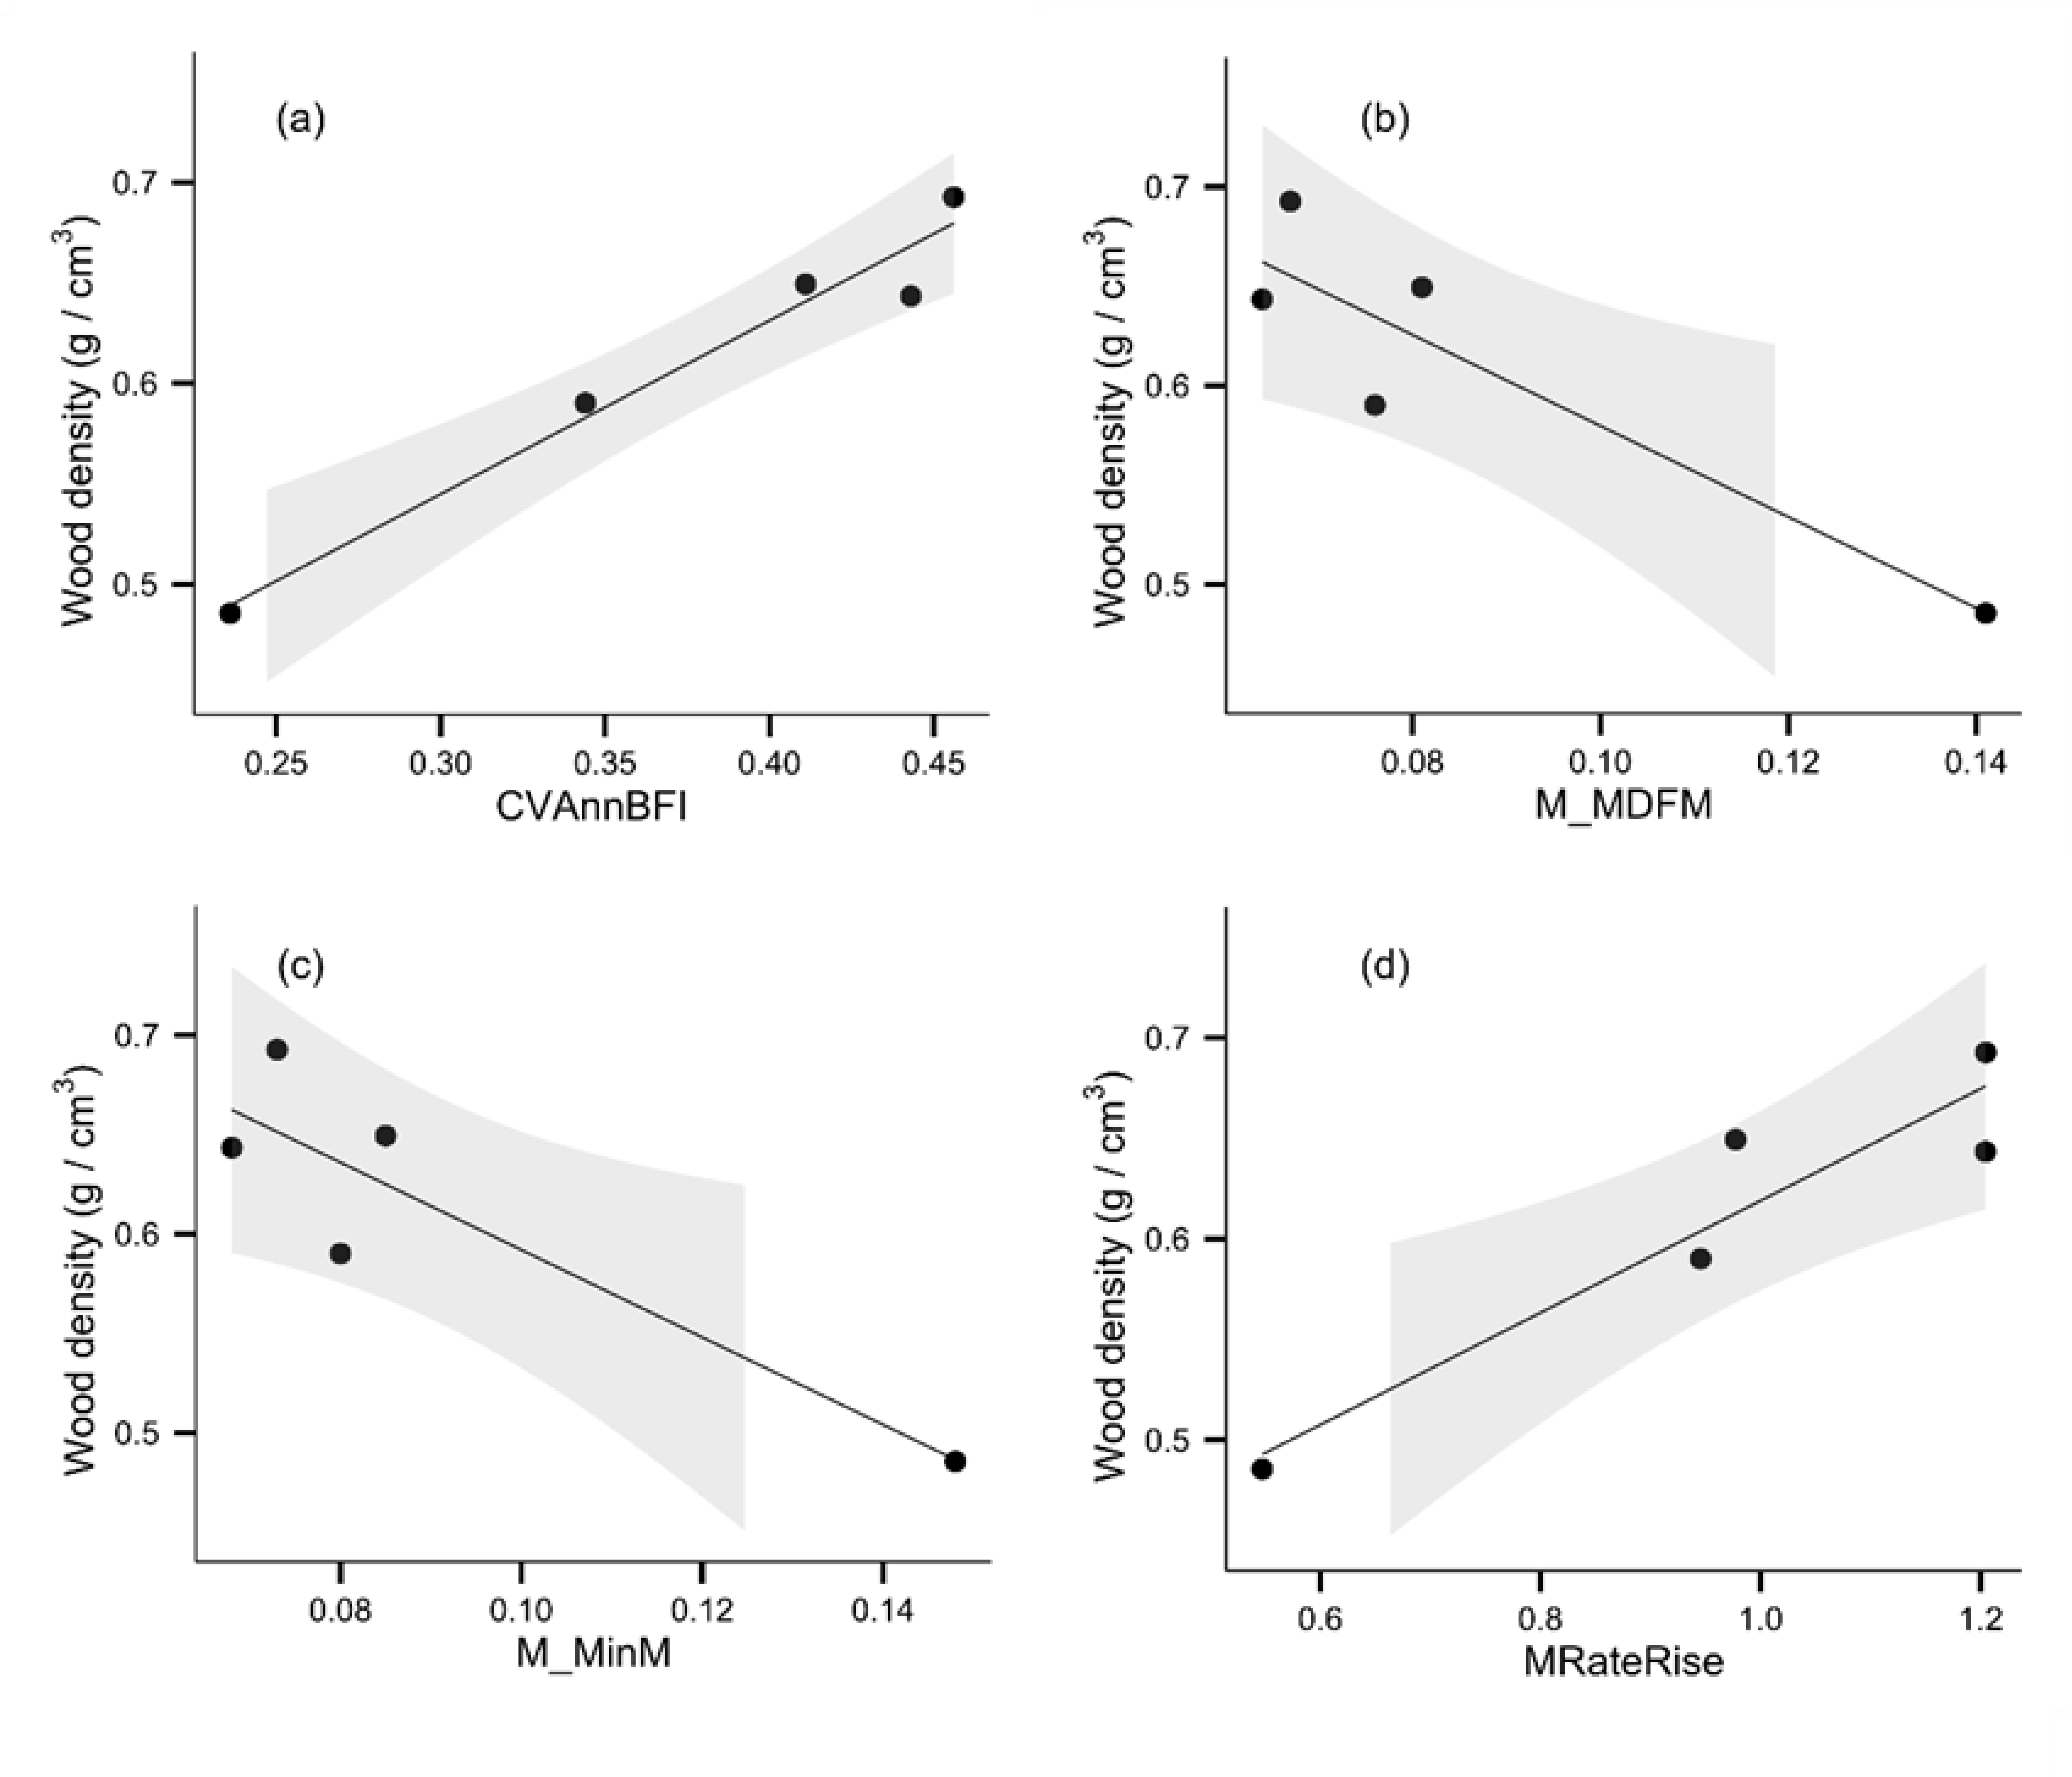
\includegraphics[width=\textwidth,keepaspectratio=true]{Ch2figS1.png} % figures can be in pdf, png, jpeg or eps format
\caption[Relationships between wood density of \textit{Casuarina cunninghamiana} and hydrological metrics]{\small{Relationships between wood density of \textit{Casuarina cunninghamiana} and hydrological metrics describing a.) interannual variability in baseflow index (CVAnnBFI) (R\textsuperscript{2} = 0.963 , P = 0.003); b.) contingency of monthly mean daily flow (M\_MDFM) (R\textsuperscript{2} = 0.826 , P = 0.033 ); c.) contingency of monthly minimum daily flow (M\_MinM) (R\textsuperscript{2} = 0.812 , P = 0.037 );  d.) mean flood rise rate (MRateRise)) (R\textsuperscript{2} = 0.885, P = 0.017). Shaded areas depict the 95 \% confidence interval around the regression model.}}
\label{Ch2sup_F1} % label for cross-referencing
\end{center}
\end{figure}   
\clearpage
\clearpage

\chapter[Appendix 2a (Summaries of environmental data, supp. Ch3)]{Summaries of environmental data, supp. Ch3}

\begin{landscape}
\begin{table}[ht]
\tiny
\centering
\caption[Location and characteristics of field sites.]{\small{Location and characteristics of field sites.}} \\
\label{Ch3sup1_T1}
{\tabulinesep=1.2mm
%\begin{tabu} to \linewidth {m{3.2cm}m{5cm}X}
\begin{tabu} to \linewidth {lm{8cm}XXXX}
\hline
\textit{Site} & \textit{Gauge Name} & \textit{Longitude} & \textit{Latitude} & \textit{Catchment area (km\textsuperscript{2})} & \textit{Elevation (m asl)} \\
\hline
1 & Mammy Johnsons River at Pikes Crossing & 151.979 & -32.244 & 158 & 104 \\
2 & Wallagaraugh River at Princes Highway & 149.714 & -37.371 & 477 & 35 \\
3 & Genoa River at Bondi & 149.321 & -37.174 & 234 & 417 \\
4 & Wadbilliga River at Wadbilliga & 149.694 & -36.259 & 126 & 201 \\
5 & Tuross River D/S Wadbilliga Junction & 149.761 & -36.197 & 918 & 79 \\
6 & Tuross River at Belowra & 149.709 & -36.201 & 564 & 105 \\
7 & Jacobs River at Jacobs Ladder & 148.427 & -36.727 & 184 & 343 \\
8 & Nariel Creek at Upper Nariel & 147.826 & -36.444 & 261 & 711 \\
9 & Gibbo River at Gibbo Park & 147.709 & -36.756 & 390 & 515 \\
10 & Snowy Creek at Below Granite Flat & 147.413 & -36.569 & 416 & 331 \\
11 & Mann River at Mitchell & 152.105 & -29.695 & 890 & 401 \\
12 & Cataract Creek at Sandy Hill & 152.217 & -28.934 & 237 & 595 \\
13 & Sportsmans Creek at Gurranang Siding & 152.981 & -29.467 & 205 & 13 \\
14 & Goodradigbee River at Brindabella & 148.731 & -35.421 & 432 & 510 \\
15 & Jilliby Creek at U/S Wyong River & 151.389 & -33.246 & 93 & 39 \\
\hline
\end{tabu}}
\end{table}
\end{landscape}
\clearpage


\begin{table}[ht]
\tiny
\centering
\caption[Importance of principal components (hydrology PCA).]{\small{Importance of components, from Principal Components Analysis of the set of 23 hydrological metrics used as explanatory variables in this study.}}\\
\label{Ch3sup1_T2}
{\tabulinesep=1.2mm
%\begin{tabu} to \linewidth {m{3.2cm}m{5cm}X}
\begin{tabu} to \linewidth {lm{3cm}XXXX}
\hline
& \textit{PC1} & \textit{PC2} & \textit{PC3} & \textit{PC4} & \textit{PC5}   \\
\hline
Standard deviation & 3.848 & 1.824 & 1.377 & 0.935 & 0.788 \\
Proportion of variance & 0.644 & 0.145 & 0.082 & 0.038 & 0.027 \\
Cumulative proportion & 0.644 & 0.788 & 0.871 & 0.909 & 0.936 \\
\hline
\end{tabu}}
\end{table}

\begin{table}[ht]
\tiny
\centering
\caption[Loadings across principal components (hydrology PCA).]{\small{Loadings across principal components for the set of 23 hydrological metrics used in this study.}}\\
\label{Ch3sup1_T3}
{\tabulinesep=1.2mm
%\begin{tabu} to \linewidth {m{3.2cm}m{5cm}X}
\begin{tabu} to \linewidth {m{4cm}XXXXX}
\hline
\textit{metric} & \textit{PC1} & \textit{PC2} & \textit{PC3} & \textit{PC4} & \textit{PC5} \\
\hline
HSPeak & -0.24 & 0.09 & 0.23 & 0.13 & 0.02 \\
MDFAnnHSNum & -0.08 & -0.46 & -0.08 & -0.39 & 0.03 \\
CVAnnHSNum & 0.00 & 0.40 & -0.34 & 0.43 & 0.06 \\
CVAnnHSPeak & -0.19 & 0.06 & -0.42 & -0.22 & 0.03 \\
MRateRise & -0.22 & -0.18 & 0.20 & 0.18 & 0.12 \\
MRateFall & -0.21 & -0.25 & 0.10 & 0.22 & -0.02 \\
CVAnnMRateRise & -0.22 & 0.26 & -0.02 & -0.15 & 0.02 \\
CVAnnMRateFall & -0.24 & 0.14 & 0.08 & -0.05 & 0.22 \\
AS20YrARI & -0.25 & 0.02 & 0.01 & 0.05 & -0.02 \\
C\_MDFM & 0.24 & -0.10 & -0.14 & 0.12 & 0.24 \\
M\_MDFM & 0.25 & 0.01 & 0.02 & 0.09 & -0.30 \\
C\_MinM & 0.24 & -0.07 & -0.15 & 0.19 & 0.14 \\
M\_MinM & 0.22 & 0.11 & 0.10 & 0.10 & -0.53 \\
C\_MaxM & 0.02 & -0.43 & 0.33 & 0.27 & 0.10 \\
M\_MaxM & 0.25 & -0.02 & 0.00 & 0.07 & -0.01 \\
MDFMDFSpring & 0.24 & 0.08 & 0.11 & -0.19 & 0.19 \\
MDFMDFSummer & -0.18 & -0.19 & -0.44 & 0.19 & 0.07 \\
MDFMDFAutumn & -0.23 & -0.13 & -0.04 & 0.17 & -0.42 \\
MDFMDFWinter & 0.14 & 0.30 & 0.40 & -0.13 & 0.23 \\
CVMDFSpring & -0.22 & 0.10 & 0.20 & 0.35 & 0.14 \\
CVMDFSummer & -0.22 & 0.11 & 0.14 & -0.20 & -0.42 \\
CVMDFAutumn & -0.24 & 0.02 & 0.01 & -0.24 & 0.09 \\
CVMDFWinter & -0.21 & 0.22 & 0.03 & 0.08 & 0.06 \\
\hline
\end{tabu}}
\end{table}

\begin{table}[ht]
\tiny
\centering
\caption[Summary statistics for hydrological variables.]{\small{Summary statistics for hydrological variables. From left: minimum, maximum, mean and standard deviation.}}\\
\label{Ch3sup1_T4}
{\tabulinesep=1.2mm
%\begin{tabu} to \linewidth {m{3.2cm}m{5cm}X}
\begin{tabu} to \linewidth {m{4cm}XXXX}
\hline
\textit{metric} & \textit{min} & \textit{max} & \textit{mean} & \textit{sd} \\
\hline
HSPeak & 5.38 & 29.81 & 16.67 & 8.34 \\
MDFAnnHSNum & 2.8 & 5.93 & 4.1 & 0.96 \\
CVAnnHSNum & 0.48 & 0.84 & 0.74 & 0.11 \\
CVAnnHSPeak & 0.24 & 1.47 & 0.69 & 0.34 \\
MRateRise & 0.2 & 1.99 & 0.91 & 0.57 \\
MRateFall & 0.07 & 0.8 & 0.34 & 0.23 \\
CVAnnMRateRise & 0.43 & 1.18 & 0.85 & 0.25 \\
CVAnnMRateFall & 0.41 & 1.46 & 0.9 & 0.34 \\
AS20YrARI & 17.94 & 209.99 & 126.13 & 81.19 \\
C\_MDFM & 0.05 & 0.31 & 0.14 & 0.09 \\
M\_MDFM & 0.06 & 0.2 & 0.12 & 0.05 \\
C\_MinM & 0.01 & 0.27 & 0.12 & 0.08 \\
M\_MinM & 0.07 & 0.16 & 0.11 & 0.03 \\
C\_MaxM & 0.19 & 0.44 & 0.28 & 0.09 \\
M\_MaxM & 0.04 & 0.18 & 0.09 & 0.06 \\
MDFMDFSpring & 0.19 & 1.81 & 1.02 & 0.55 \\
MDFMDFSummer & 0.42 & 1.49 & 0.88 & 0.33 \\
MDFMDFAutumn & 0.28 & 1.82 & 1 & 0.52 \\
MDFMDFWinter & 0.64 & 1.44 & 1.08 & 0.25 \\
CVMDFSpring & 0.36 & 2.1 & 1.12 & 0.54 \\
CVMDFSummer & 0.6 & 1.66 & 1.15 & 0.39 \\
CVMDFAutumn & 0.48 & 1.49 & 1.07 & 0.35 \\
CVMDFWinter & 0.46 & 1.99 & 1.05 & 0.46 \\
\hline
\end{tabu}}
\end{table}
\clearpage

\textbf{Bioclimatic variables assessed for relationships with FDis:}

\small{Annual Mean Temperature

Mean Diurnal Range (Mean of monthly (max temp - min temp))

Isothermality (BIO2/BIO7) (* 100)

Temperature Seasonality (standard deviation * 100)

Max Temperature of Warmest Month

Min Temperature of Coldest Month

Temperature Annual Range (BIO5-BIO6)

Mean Temperature of Wettest Quarter

Mean Temperature of Driest Quarter

Mean Temperature of Warmest Quarter

Mean Temperature of Coldest Quarter

Annual Precipitation

Precipitation of Wettest Month

Precipitation of Driest Month

Precipitation Seasonality (Coefficient of Variation)

Precipitation of Wettest Quarter

Precipitation of Driest Quarter

Precipitation of Warmest Quarter

Precipitation of Coldest Quarter}

\newpage

\textbf{Edaphic variables assessed for relationships with FDis:}

\small{Available Water Capacity

Bulk Density – Whole Earth (g cm\textsuperscript{-3})

Clay (\%)

Depth of Regolith (m)

Depth of Soil (m)

Effective Cation Exchange Capacity (meq / 100 g)

Total Nitrogen (\%)

pH – CaCl2 

Total Phosphorous (\%)

Silt (\%)

Sand (\%)

Organic Carbon (\%)}

\newline
Further information on soil variables can be found at: \newline
\url{http://www.clw.csiro.au/aclep/soilandlandscapegrid} (accessed 09/06/2015)

\clearpage

\chapter[Appendix 2b (supplementary to Chapter 3)]{Appendix 2b (supplementary to Chapter 3)}

\begin{landscape}
\begin{table}[ht]
\tiny
\centering
\caption[Data density information for trait dataset.]{\small{Data density information for trait dataset. Coverage describes the total proportional coverage at a site for which species were included in the analysis. Density values for each trait describe the proportional coverage at a site for which data for that trait were included in the analysis. N.B. leaf narrowness and wood density were not available for grasses or ferns; seed mass and flowering period were also not available for ferns.}} \\
\label{Ch3sup2_T1} \\
{\tabulinesep=1.2mm
\begin{tabu} to \linewidth {XXXXXXXX}
\hline
\textit{site} & \textit{coverage} & \textit{wood density} & \textit{max. height} & \textit{seed mass} & \textit{SLA} & \textit{flowering period} & \textit{leaf narrowness} \\
\hline
1 & 0.98 & 0.615 & 1 & 0.846 & 1 & 0.923 & 0.692 \\
2 & 0.959 & 0.333 & 1 & 0.667 & 1 & 0.667 & 0.333 \\
3 & 0.949 & 0.455 & 1 & 0.727 & 1 & 0.727 & 0.545 \\
4 & 0.903 & 0.4 & 1 & 0.867 & 1 & 0.867 & 0.6 \\
5 & 0.968 & 0.455 & 1 & 1 & 1 & 1 & 0.545 \\
6 & 0.964 & 0.7 & 1 & 1 & 1 & 1 & 0.7 \\
7 & 1 & 0.5 & 1 & 1 & 0.9 & 1 & 0.7 \\
8 & 1 & 0.529 & 1 & 0.882 & 1 & 0.882 & 0.765 \\
9 & 0.988 & 0.474 & 1 & 0.842 & 1 & 0.842 & 0.737 \\
10 & 0.976 & 0.583 & 1 & 0.917 & 1 & 0.917 & 0.667 \\
11 & 0.96 & 0.188 & 1 & 1 & 0.938 & 1 & 0.688 \\
12 & 0.992 & 0.381 & 1 & 0.952 & 0.952 & 0.952 & 0.714 \\
13 & 0.935 & 0.55 & 0.95 & 0.9 & 1 & 0.9 & 0.7 \\
14 & 1 & 0.636 & 1 & 1 & 1 & 1 & 1 \\
15 & 0.963 & 0.455 & 1 & 0.909 & 0.909 & 0.909 & 0.727 \\
\hline
\end{tabu}}
\end{table}
\end{landscape}
\clearpage

\begin{table}[ht]
\tiny
\centering
\caption[Summary statistics for trait dataset.]{\small{Summary statistics for trait dataset. From left: minimum, maximum, mean and standard deviation.}} \\
\label{Ch3sup2_T2} \\
{\tabulinesep=1.2mm
\begin{tabu} to \linewidth {p{5cm}XXXX}
\hline
\textit{trait} & \textit{min} & \textit{max} & \textit{mean} & \textit{sd} \\
\hline
Max. height (m) & 0.2 & 50 & 10.47 & 13.18 \\
Seed mass (mg) & 0.04 & 323.99 & 16.55 & 45.06 \\
SLA (m\textsuperscript{2} / kg) & 1.41 & 63.27 & 17.93 & 14 \\
Flowering period length \newline(proportion of year) & 0.17 & 1 & 0.45 & 0.24 \\
Leaf narrowness (unitless ratio) & 0.59 & 233.33 & 9.86 & 32.53 \\
Wood density (g / cm\textsuperscript{3}) & 0.33 & 0.95 & 0.61 & 0.13 \\
\hline
\end{tabu}}
\end{table}


\begin{table}[ht]
\tiny
\centering
\caption[Importance of principal components (trait dataset, all traits).]{\small{Importance of principal components PC1 – PC5 from Principal Components Analysis of trait dataset, using species with data available for all traits (55 species).}} \\
\label{Ch3sup2_T3} \\
{\tabulinesep=1.2mm
\begin{tabu} to \linewidth {p{4cm}XXXXXX}
\hline
&                      \textit{PC1}  & \textit{PC2}    & \textit{PC3}    & \textit{PC4}    & \textit{PC5}    & \textit{PC6}            \\ 
\hline
Standard deviation     & 1.3938 & 1.0962 & 1.0827 & 0.9247 & 0.7438 & 0.52457 \\
Proportion of variance & 0.3238 & 0.2003 & 0.1954 & 0.1425 & 0.0922 & 0.04586 \\
Cumulative  proportion & 0.3238 & 0.5240 & 0.7194 & 0.8619 & 0.9541 & 1      \\
\hline
\end{tabu}}
\end{table}

\begin{table}[ht]
\tiny
\centering
\caption[Importance of principal components (trait dataset, only traits will full data coverage).]{\small{Importance of principal components PC1 – PC5 from Principal Components Analysis of trait dataset, using species with data available for SLA, maximum height, seed mass and flowering period length (97 species).}} \\
\label{Ch3sup2_T4} \\
{\tabulinesep=1.2mm
\begin{tabu} to \linewidth {p{4cm}XXXX}
\hline
& \textit{PC1}  & \textit{PC2}    & \textit{PC3}    & \textit{PC4}   \\
\hline
Standard deviation & 1.4160 & 1.0016 & 0.8326 & 0.54649 \\
Proportion of variance & 0.5012 & 0.2508 & 0.1733 & 0.07466 \\
Cumulative  proportion & 0.5012 & 0.7520 & 0.9253 & 1  \\
\hline
\end{tabu}}
\end{table}

\clearpage

\clearpage

\chapter[Appendix 2c (Univariate regression stats, supp. Ch3)]{Appendix 2c (Univariate regression stats, supp. Ch3)}

\begin{table}[ht]
\tiny
\centering
\caption[Statistics for univariate linear regression models.]{\small{Statistics for univariate linear regression models comparing FDis with hydrological metrics. p.adj represents p values which have been adjusted to control the false discovery rate. Relationships which remained significant following adjustment are shown in bold typeface. * All models are linear apart from M\_MinM and CVMDFSummer, for which a quadratic model (df = 2,12) provided a substantially better fit.}} \\
\label{Ch3sup4_T1} \\
{\tabulinesep=1.2mm
\begin{tabu} to \linewidth {p{4cm}XXXX}
\hline
\textit{metric} & \textit{p} & \textit{p.adj} & \textit{R2} & \textit{F(1,13)} \\
\hline
CVAnnHSPeak & 0.001 & 0.0152 & 0.577 & 17.750 \\
M\_MinM & 0.0094 & 0.0278 & 0.540 & *7.0560 \\
MDFMDFSummer & 0.0031 & 0.023 & 0.503 & 13.170 \\
CVMDFSummer & 0.0218 & 0.0325 & 0.472 & *5.3560 \\
CVMDFWinter & 0.0096 & 0.0278 & 0.414 & 9.194 \\
CVAnnMRateRise & 0.011 & 0.0278 & 0.403 & 8.781 \\
CVAnnMRateFall & 0.0129 & 0.0278 & 0.390 & 8.299 \\
MDFMDFSpring & 0.0134 & 0.0278 & 0.386 & 8.180 \\
AS20YrARI & 0.0148 & 0.0278 & 0.377 & 7.879 \\
M\_MDFM & 0.0209 & 0.0325 & 0.347 & 6.908 \\
M\_MaxM & 0.0258 & 0.0325 & 0.328 & 6.330 \\
CVMDFSpring & 0.026 & 0.0325 & 0.327 & 6.313 \\
CVMDFAutumn & 0.0342 & 0.0386 & 0.301 & 5.595 \\
CVAnnHSNum & 0.036 & 0.0386 & 0.296 & 5.468 \\
HSPeak & 0.0648 & 0.0648 & 0.238 & 4.069 \\
MDFMDFWinter & 0.0881 & 0.078 & 0.207 & 3.401 \\
C\_MaxM & 0.0885 & 0.078 & 0.207 & 3.392 \\
C\_MDFM & 0.1086 & 0.0861 & 0.186 & 2.968 \\
MDFMDFAutumn & 0.1091 & 0.0861 & 0.185 & 2.959 \\
C\_MinM & 0.1361 & 0.1021 & 0.163 & 2.524 \\
MRateRise & 0.1556 & 0.1072 & 0.149 & 2.272 \\
MRateFall & 0.1572 & 0.1072 & 0.148 & 2.253 \\
MDFAnnHSNum & 0.727 & 0.4741 & 0.010 & 0.127 \\
\hline
\end{tabu}}
\end{table}

\clearpage


\clearpage


\chapter[Appendix 3 (supplementary to Chapters 2 and 3)]{Appendix 3 (supplementary to Chapters 2 and 3)}

\section*{Study regions and biophysical characteristics of study sites in Chapters 2-3}

This section describes the biophysical characteristics of study sites used in Chapters 2 and 3. For further information about study sites used in Chapter 4, the reader is referred to Arthington et al. (2012).

%%%% FIGURE 1
\begin{figure}[ht]
\begin{center}
\includegraphics[width=12cm,keepaspectratio=true]{Ch6map.png} % figures can be in pdf, png, jpeg or eps format
\caption[Map of study areas described in Chapters 2-4.]{\small{Map showing study areas, and geographical distribution of field sites described in Chapters 2 \& 3 (lower left) and 4 (lower right) (Google Maps 2015).}\label{fig:Ch6_F1}}
%\label{Ch6_F1} % label for cross-referencing
\end{center}
\end{figure}   
\clearpage

\begin{landscape}
\begin{table}[ht]
\tiny
\centering
\caption[Biogeographical attributes of study sites.]{\small{Biogeographical attributes of study sites.}}
\label{biophysical_F1}
{\tabulinesep=1.2mm
%\begin{tabu} to \linewidth {m{3.2cm}m{5cm}X}
\begin{tabu} to \linewidth {m{4cm}m{3cm}m{3cm}m{2cm}m{2cm}m{2cm}m{2cm}}
\hline
\textit{Site}  & \textit{IBRA region}  & \textit{Koppen climate zone} & \textit{Mean annual rainfall (mm)} & \textit{Mean annual temperature (\textsuperscript{o}C)} & \textit{Upstream catchment area (m2)} & \textit{elevation (m asl)} \\
\hline
Mammy Johnsons River at Pikes Crossing & NSW North Coast          & Warm summer, cold winter      & 1136                      & 17.5                         & 158                          & 104               \\
Wallagaraugh River at Princes Highway  & South East Corner        & Warm summer, cold winter      & 925                       & 14.9                         & 477                          & 35                \\
Genoa River at Bondi                   & South East Corner        & Warm summer, cold winter      & 815                       & 13.0                         & 234                          & 417               \\
Wadbilliga River at Wadbilliga         & South East Corner        & Warm summer, cold winter      & 842                       & 14.8                         & 126                          & 201               \\
Tuross River D/S Wadbilliga Junction   & South East Corner        & Warm summer, cold winter      & 843                       & 15.4                         & 918                          & 79                \\
Tuross River at Belowra                & South East Corner        & Warm summer, cold winter      & 831                       & 15.4                         & 564                          & 105               \\
Jacobs River at Jacobs Ladder          & South Eastern Highlands  & Mild-warm summer, cold winter & 563                       & 13.9                         & 184                          & 343               \\
Nariel Creek at Upper Nariel           & South Eastern Highlands  & Mild-warm summer, cold winter & 982                       & 12.8                         & 261                          & 711               \\
Gibbo River at Gibbo Park              & South Eastern Highlands  & Mild-warm summer, cold winter & 919                       & 12.5                         & 390                          & 515               \\
Snowy Creek at Below Granite Flat      & South Eastern Highlands  & Mild-warm summer, cold winter & 1030                      & 13.8                         & 416                          & 331               \\
Mann River at Mitchell                 & New England Tablelands   & Warm summer, cold winter      & 865                       & 16.7                         & 890                          & 401               \\
Cataract Creek at Sandy Hill           & New England Tablelands   & Warm summer, cold winter      & 1019                      & 16.4                         & 237                          & 595               \\
Sportsmans Creek at Gurranang Siding   & South Eastern Queensland & Warm humid summer             & 1094                      & 19.1                         & 205                          & 13                \\
Goodradigbee River at Brindabella      & South Eastern Highlands  & Mild-warm summer, cold winter & 976                       & 12.7                         & 432                          & 510               \\
Jilliby Creek at U/S Wyong River       & Sydney Basin             & Warm summer, cold winter      & 1110                      & 17.7                         & 93                           & 39          \\     
\hline
\end{tabu}}
\end{table}
\end{landscape}
\clearpage





\begin{landscape}
\tiny
{\tabulinesep=1.2mm
%\begin{tabu} to \linewidth {m{3.2cm}m{5cm}X}
\begin{longtabu} to \linewidth {m{3cm}m{1.5cm}XXX}
\caption[Vegetation charactersitics of study sites.]{\small{Vegetation charactersitics of study sites.}}
\label{biophysical_F2}
\hline
\textit{Site}  & \textit{Canopy height (m)} & \textit{Vegetation structure}  & \textit{Dominant species} & \textit{Site history}  \\
\endfirsthead

\hline
\textit{Site}  & \textit{Canopy height (m)} & \textit{Vegetation structure}  & \textit{Dominant species} & \textit{Site history}  \\ \hline
\endhead
\hline
Mammy Johnsons River at Pikes Crossing & 15                & Closed canopy, abundant subcanopy and limited groundcover               & \textit{Acmena smithii, Ceratopetalum apetalum, Tristaniopsis laurina}                                                                             & Adjacent smallhold grazing, unfenced, possible historic clearing                                                                                                                                       \\
Wallagaraugh River at Princes Highway  & 12                & Closed low canopy, fern dominated groundcover layer                     & \textit{Tristaniopsis laurina, Doodia aspera}                                                                                                      & Undisturbed, evidenced by numerous large Eucalyptus viminalis individuals adjacent to site                                                                                                             \\
Genoa River at Bondi                   & 30                & Tall open canopy, abundant subcanopy and groundcover                    & \textit{Eucalyptus viminalis, Pomaderris aspera, Leptospermum brevipes, Calochlaena dubia}                                                         & Undisturbed, within South East Forest National Park                                                                                                                                                    \\
Wadbilliga River at Wadbilliga         & 30                & Tall open canopy, abundant shrubs and groundcover                       & \textit{Casuarina cunninghamiana, Eucalyptus cypellocarpa, Acacia floribunda, Melicytus dentatus, Microlaena stipoides}                            & Within Wadbilliga National Park. Mature forest, but historical clearing / pastoral land use possible.                                                                                                  \\
Tuross River D/S Wadbilliga Junction   & 30                & Open forest, shrub and groundcover layers dominant, scattered emergents & \textit{Casuarina cunninghamiana, Eucalyptus elata, Tristaniopsis laurina, Acacia floribunda, Backhousia myrtifolia, Microlaena stipoides}         & Within Wadbilliga National Park. Mature forest with large emergents, but historical clearing / pastoral land usepossible.                                                                              \\
Tuross River at Belowra                & 12                & Riparian scrub with emergent streamside \textit{Casuarina} forest                & \textit{Casuarina cunninghamiana, Acacia floribunda, Leptospermum brevipes}                                                                        & Within Wadbilliga National Park. Mature riparian scrub vegetation, but historical clearing / pastoral land use possible.                                                                               \\
Jacobs River at Jacobs Ladder          & 14                & Open woodland with some emergent Eucalypts                              & \textit{Eucalyptus rubida, Acacia dealbata, Rubus fruticosus}                                                                                      & Within Kosciuzko National Park. In recovery following 2003 fires.                                                                                                                                      \\
Nariel Creek at Upper Nariel           & 40                & Open forest, dense fern groundcover                                     & \textit{Eucalyptus camphora subsp. humeana, Acacia melanoxylon, Rubus fruticosus, Blechnum nudum}                                                  & Mature forest, some clearing adjacent to riparian corridor. Historical clearing / pastoral land use possible.                                                                                          \\
Gibbo River at Gibbo Park              & 35                & Open forest, abundant shrub layer                                       & \textit{Eucalyptus radiata, Acacia dealbata, Lomatia myricoides, Poa labillardierei var labillardierei}                                            & Largely undisturbed, some evidence of fire. Within Alpine National Park. Very large emergent \textit{Eucalyptus viminalis} (\textgreater2m DBH) present.                                                                                       \\ 
Snowy Creek at Below Granite Flat      & 20                & Riparian scrub with low emergent Eucalypts                              & \textit{Eucalyptus camphora subsp. camphora, Eucalyptus stellulata, Coprosma quadrifida, Bursaria spinosa, Leptospermum brevipes}                  & Within Victoria State Forest, clearing for forestry was evident downstream.                                                                                                                            \\
Mann River at Mitchell                 & 30                & Open grassy forest                                                      & \textit{Casuarina cunninghamiana, Eucalyptus ampifolia, Lomandra longifolia, Microlaena stipoides}                                                 & Within Mann River Nature Reserve. Large flood occurred in 2011, historical clearing / pastoral land use is possible.                                                                                   \\
Cataract Creek at Sandy Hill           & 30                & Open forest, abundant shrubs and grassy areas                           & \textit{Casuarina cunninghamiana, Eucalyptus tereticornis, Melicytus dentatus, Lomandra hystrix, Pennisetum clandestinum}                          & Within NSW conservation land, although opposite side of river was cleared pastoral land. Large flood occurred in 2011.                                                                                 \\
Sportsmans Creek at Gurranang Siding   & 25                & Closed forest                                                           & \textit{Lophostemon suaveolens, Alphitonia excelsa, Casuarina glauca, Calochlaena dubia, Oplismenus imbecillis}                                    & Riparian corridor remnant vegetation. Adjacent to Gunnarang State Conservation Area. Large (\textgreater2m DBH) emergent \textit{Lophostemon suaveolens} individuals indicate relatively undisturbed condition. \\
Goodradigbee River at Brindabella      & 25                & Closed forest, abundant shrub layer with sparse groundcover             & \textit{Eucalyptus radiata, Eucalyptus viminalis, Acacia dealbata, Acacia pravissima, Hovea asperifolia subsp. asperifolia, Leptospermum brevipes} & Within Kosciuzko National Park. Fire occurred in 2010.                                                                                                                                                 \\
Jilliby Creek at U/S Wyong River       & 50                & Vine thickets with emergent Eucalypts                                   & \textit{Eucalyptus tereticornis, Eucalyptus resinifera, Commersonia fraseri, Ripogonum album, Lomandra longifolia}                                 & Riparian corridor remnant vegetation. Large emergent \textit{Eucalyptus} individuals (40-50 m tall) indicate relatively undisturbed condition.                                                                 
\hline
\end{longtabu}}
\end{landscape}
\clearpage

PHOTOS









\clearpage

%
%%%%%%%%%%%%%%%%%%%%%%%%%%%%%%%%%%%%%%%%%%%%%%%%%%%%%%%%%%%%%%%%%%%%%%
% Tina Dissertation
% December 2013, modified to Template June 2015
%%%%%%%%%%%%%%%%%%%%%%%%%%%%%%%%%%%%%%%%%%%%%%%%%%%%%%%%%%%%%%%%%%%%%%
% Documentclass Memoir 
% check memman.pdf for help and information
%%%%%%%%%%%%%%%%%%%%%%%%%%%%%%%%%%%%%%%%%%%%%%%%%%%%%%%%%%%%%%%%%%%%%%
\documentclass[openright,12pt,a4paper]{memoir} 
\usepackage{graphicx}
%\usepackage[utf8]{inputenc} % set input encoding to utf8
\usepackage{array} % for tables 
\usepackage{multirow} % for tables 
\usepackage{multicol} % for tables
\usepackage{tabularx} % for tables
\usepackage{booktabs}
\usepackage{cite}
\usepackage{tabularx}
\usepackage[round]{natbib}
\usepackage{threeparttable}
\DisemulatePackage{setspace}
\usepackage{setspace}
\usepackage{longtable}
\usepackage{tabu}
\usepackage{pdflscape}
\usepackage{caption}
%\usepackage{lmodern}


% defines new column type
\newcolumntype{Z}{$>${\raggedright\arraybackslash}X}

% add a little vertical padding to cramped tables
\setlength{\extrarowheight}{2pt}


%%%%%%%%%%%%%%%%%%%%%%%%%%%%%%%%%%%%%%%%%%%%%%%%%%%%%%%%%%%%%%%%%%
%%% Examples of Memoir customization
%%% enable, disable or adjust these as desired

%%% PAGE DIMENSIONS
% a4paper is by default 210mm wide and 279 mm wide

% default document in memoir is twoside (recto-verso) and openright (new chapter begins on recto page)

% size of the text area
  \settrims{0pt}{0pt}
  \settypeblocksize{230mm}{147mm}{*}
  \setlength{\spinemargin}{27mm}
  \setlength{\foremargin}{36mm}
%\setulmargins{35mm}{45mm}{*}
%\setlength{\marginparwidth}{0mm}
%\setlength{\marginparsep}{0mm}
%\setlength{\textwidth}{140mm}
%\settrimmedsize{0.9\stockheight}{0.9\stockwidth}{*}
%\setlength{\trimtop}{0pt}
%\setlength{\trimedge}{0pt}
%\addtolength{\trimedge}{-\paperwidth}
%\settypeblocksize{*}{\lxvchars}{1.618} % we want to the text block to have golden proportionals
  \setulmargins{*}{*}{1.618} % 50pt upper margins
%\setlrmargins{*}{*}{1.3}
%  \setlrmargins{*}{*}{1} % golden ratio again for left/right margins
  \setheaderspaces{*}{*}{1.618}
  \checkandfixthelayout % to make sure that the layout parameters make sense

%\addtolength{\textwidth}{0cm}
%\addtolength{\textheight}{1.5cm}
%\addtolength{\textwidth}{-2cm}
%\addtolength{\textheight}{+0.5cm}

%%% \maketitle CUSTOMISATION
% For more than trivial changes, you may as well do it yourself in a titlepage environment
%\pretitle{\begin{center}\sffamily\Huge\MakeUppercase}
%\posttitle{\par\end{center}\vskip 0.5em}

%%% ToC (table of contents) APPEARANCE
  \maxtocdepth{subsection} % include subsections
%\renewcommand{\cftchapterpagefont}{}
%\renewcommand{\cftchapterfont}{}     % no bold!

%%% HEADERS & FOOTERS
  \pagestyle{headings} % try also: empty , plain , headings , ruled , Ruled , companion

%%% CHAPTERS
  \chapterstyle{southall} % try also: default , section , hangnum , companion , article, demo

  \renewcommand{\chaptitlefont}{\LARGE\sffamily\raggedright} % set sans serif chapter title font
  \renewcommand{\chapnumfont}{\LARGE\sffamily\raggedright} % set sans serif chapter number font

%%% TABLES
  \newcolumntype{C}[1]{$>${\centering}m{#1}} % defines the default layout of the tables (C$=$centerling, L$=$left)
  \newcolumntype{L}[1]{$>${\centering}m{#1}}

%%% SECTIONS
%\hangsecnum % hang the section numbers into the margin to match \chapterstyle{hangnum}
  \maxsecnumdepth{section} % number subsections

  \setsecheadstyle{\Large\sffamily\raggedright} % set sans serif section font
  \setsubsecheadstyle{\large\sffamily\raggedright} % set sans serif subsection font

%%% Abstract
  \setlength{\absleftindent}{0mm}
  \setlength{\absrightindent}{0mm}

  \renewcommand{\absnamepos}{center}
  \setlength{\abstitleskip}{+0cm}

%%% Captions

%\DeclareCaptionFont{tiny}{\tiny}
%\captionsetup{font$=$tiny, labelfont$=$tiny}
%\usepackage[font$=${tiny}, labelfont$=${tiny}]{caption}
%\usepackage[font$=$sf, labelfont$=${sf,bf}, margin$=$1cm]{caption}
%\captionsetup{font$=$scriptsize,labelfont$=$scriptsize}

%\usepackage[textfont$=${tiny}, labelfont$=${tiny}]{caption}

 % \captionnamefont{\tiny}
 %\captiontitlefont{\tiny}

%% END Memoir customization


%%%%%%%%%%%%%%%%%%%%%%%%%%%%%%%%%%%%%%%%%%%%%%%%%%%%%%%%%%%%%%%%%%%%%%%%%%%%%%%%%%%%%%%%%%%%%%%%%%%%%%%%%%%%%%%%%%%%%%%%%%%%%%%%%%%%%%%%%%%%%
%%% BEGIN DOCUMENT

\begin{document}
\doublespacing

\Chapter[Appendix 3a]{Appendix 3a}

\begin{table}[ht]
\tiny
\centering
\caption[PCA of hydrological variables/]{Importance of components, from Principal Components Analysis of the set of 18 hydrological metrics used as explanatory variables in this study.}
\label{Ch4sup_T1}
\begin{tabu} to \textwidth {p{5cm}XXXXXX}
\hline
                       &  \textit{PC1}   & \textit{PC2}   & \textit{PC3}   & \textit{PC4}   & \textit{PC5}  \\ \hline
Standard deviation     & 2.787 & 1.995 & 1.273 & 1.079 & 0.996 \\
Proportion of variance & 0.431 & 0.221 & 0.090 & 0.065 & 0.042 \\
Cumulative proportion  & 0.431 & 0.653 & 0.743 & 0.807 & 0.862 \\ \hline
\end{tabu}
\end{table}

\begin{table}[ht]
\tiny
\centering
\caption[Loadings across principal components for hydrological metrics.]{Loadings across principal components for the set of 18 hydrological metrics used as explanatory variables in this study.}
\label{Ch4sup_T2}
\begin{tabu} to \textwidth {p{4cm}XXXXXX}
\hline
\textit{metric}         & \textit{PC1}    & \textit{PC2}    & \textit{PC3}    & \textit{PC4}    & \textit{PC5}    \\ \hline
MDFMDFWet      & -0.068 & 0.127  & -0.647 & -0.183 & 0.210  \\
MDFMDFDry      & 0.261  & -0.226 & -0.132 & -0.141 & 0.243  \\
CVMDFWet       & -0.300 & -0.102 & 0.242  & -0.194 & 0.210  \\
CVMDFDry       & -0.331 & -0.134 & 0.043  & 0.125  & -0.046 \\
HSPeak         & -0.307 & -0.001 & -0.272 & 0.190  & -0.018 \\
HSMeanDur      & 0.261  & -0.313 & -0.046 & 0.068  & -0.016 \\
CVAnnHSPeak    & -0.296 & 0.063  & -0.210 & 0.082  & 0.131  \\
CVAnnHSMeanDur & 0.141  & -0.367 & 0.150  & 0.312  & 0.029  \\
LSPeak         & -0.137 & 0.384  & -0.023 & 0.314  & 0.257  \\
LSMeanDur      & -0.283 & -0.193 & -0.067 & -0.336 & 0.205  \\
CVAnnLSPeak    & 0.095  & -0.342 & 0.069  & -0.350 & 0.330  \\
CVAnnLSMeanDur & -0.121 & -0.242 & -0.199 & 0.130  & 0.311  \\
BFI            & 0.334  & -0.020 & -0.026 & 0.205  & 0.215  \\
CVAnnBFI       & -0.250 & -0.286 & -0.139 & 0.160  & -0.235 \\
C\_MinM        & 0.200  & -0.225 & -0.403 & 0.394  & -0.045 \\
M\_MinM        & 0.172  & 0.159  & -0.211 & -0.233 & -0.451 \\
C\_MaxM        & -0.154 & -0.345 & -0.155 & -0.202 & -0.456 \\
M\_MaxM        & 0.259  & 0.175  & -0.246 & -0.283 & 0.066  \\ \hline
\end{tabu}
\end{table}


\begin{table}[ht]
\tiny
\centering
\caption[Summary statistics for trait data.]{Summary statistics for trait data.}
\label{Ch4sup_T3}
\begin{tabu}to \textwidth{p{6cm}XX}
%\begin{tabu}to \textwidth{XXX}
\hline
\textit{trait}                       & \textit{mean}   & \textit{SD}     \\ \hline

flowering duration (months) & 4.72   & 2.58   \\
leaf area (cm\textsuperscript{2})             & 28.61  & 28.05  \\
maximum height (m)          & 19.79  & 13.98  \\
seed mass (mg)              & 365.99 & 2078.8 \\
SLA (cm\textsuperscript{2}/g)                 & 15.3   & 7.42   \\
wood density (g/cm\textsuperscript{3})        & 0.609  & 0.13   \\ \hline
\end{tabu}
\end{table}

\begin{table}[ht]
\tiny
\centering
\caption[Proportional abundance of plants represented in the functional diversity analysis at each site.]{Proportional abundance of plants represented in the functional diversity analysis at each site.}
\label{Ch4sup_T4}
\begin{tabu} to \textwidth{XXXX}
\hline
\textit{site} & \textit{Total cover\newline (individuals Ha\textsuperscript{-1)}} & \textit{Represented cover\newline (individuals Ha\textsuperscript{-1})} & \textit{Proportion\newline represented} \\ \hline

1    & 8365                           & 8219                                 & 0.983                  \\
2    & 13698                          & 13643                                & 0.996                  \\
3    & 28142                          & 22487                                & 0.799                  \\
4    & 9567                           & 8177                                 & 0.855                  \\
5    & 3193                           & 3179                                 & 0.996                  \\
6    & 25237                          & 25140                                & 0.996                  \\
7    & 14409                          & 12887                                & 0.894                  \\
8    & 9458                           & 9384                                 & 0.992                  \\
9    & 16578                          & 15068                                & 0.909                  \\
10   & 12505                          & 11118                                & 0.889                  \\
11   & 42275                          & 35464                                & 0.839                  \\
12   & 9320                           & 9320                                 & 1.000                  \\
13   & 25981                          & 23881                                & 0.919                  \\
14   & 12954                          & 12007                                & 0.927                  \\
15   & 11103                          & 10882                                & 0.980                  \\
16   & 20669                          & 16540                                & 0.800                  \\
17   & 25177                          & 18199                                & 0.723                  \\
18   & 4613                           & 4219                                 & 0.915                  \\
19   & 3657                           & 3443                                 & 0.942                  \\
20   & 27249                          & 23889                                & 0.877                  \\
21   & 23301                          & 23008                                & 0.987                  \\
22   & 15639                          & 13730                                & 0.878                  \\
23   & 10855                          & 6067                                 & 0.559                  \\
24   & 17888                          & 15538                                & 0.869                  \\
25   & 3869                           & 2603                                 & 0.673                  \\
26   & 14070                          & 11862                                & 0.843                  \\
27   & 17238                          & 14213                                & 0.825                  \\
28   & 13756                          & 9638                                 & 0.701                  \\
29   & 7249                           & 7208                                 & 0.994                  \\
30   & 21555                          & 21483                                & 0.997                  \\
31   & 7296                           & 7227                                 & 0.991                  \\
32   & 5307                           & 5307                                 & 1.000                  \\
33   & 19417                          & 19046                                & 0.981                  \\
34   & 9942                           & 9782                                 & 0.984                  \\
35   & 8202                           & 8185                                 & 0.998                  \\
36   & 3745                           & 3607                                 & 0.963                  \\
37   & 13851                          & 13535                                & 0.977                  \\
38   & 18326                          & 15187                                & 0.829                  \\
39   & 8410                           & 5840                                 & 0.694                  \\
40   & 5360                           & 5283                                 & 0.986                  \\ \hline
\end{tabu}
\end{table}

\clearpage

\begin{table}[ht]
\tiny
\centering
\caption[Proportion of species for which trait values were available.]{Proportion of species included in the functional diversity analysis for which trait values were available.}
\label{Ch4sup_T5}
\begin{tabu} to \textwidth {XX}
\hline
\textit{trait}              & \textit{data density} \\ \hline

flowering duration & 0.891        \\
growth form        & 1            \\
leaf area          & 0.983        \\
maximum height     & 0.971        \\
seed mass          & 0.868        \\
SLA                & 0.661        \\
wood density       & 0.672        \\ \hline
\end{tabu}
\end{table}

\end{document}

\clearpage

\chapter[Appendix 4b (supplementary to Chapter 4)]{Appendix 4b (supplementary to Chapter 4)}

\begin{landscape}
\begin{figure}[h!]
\begin{center}
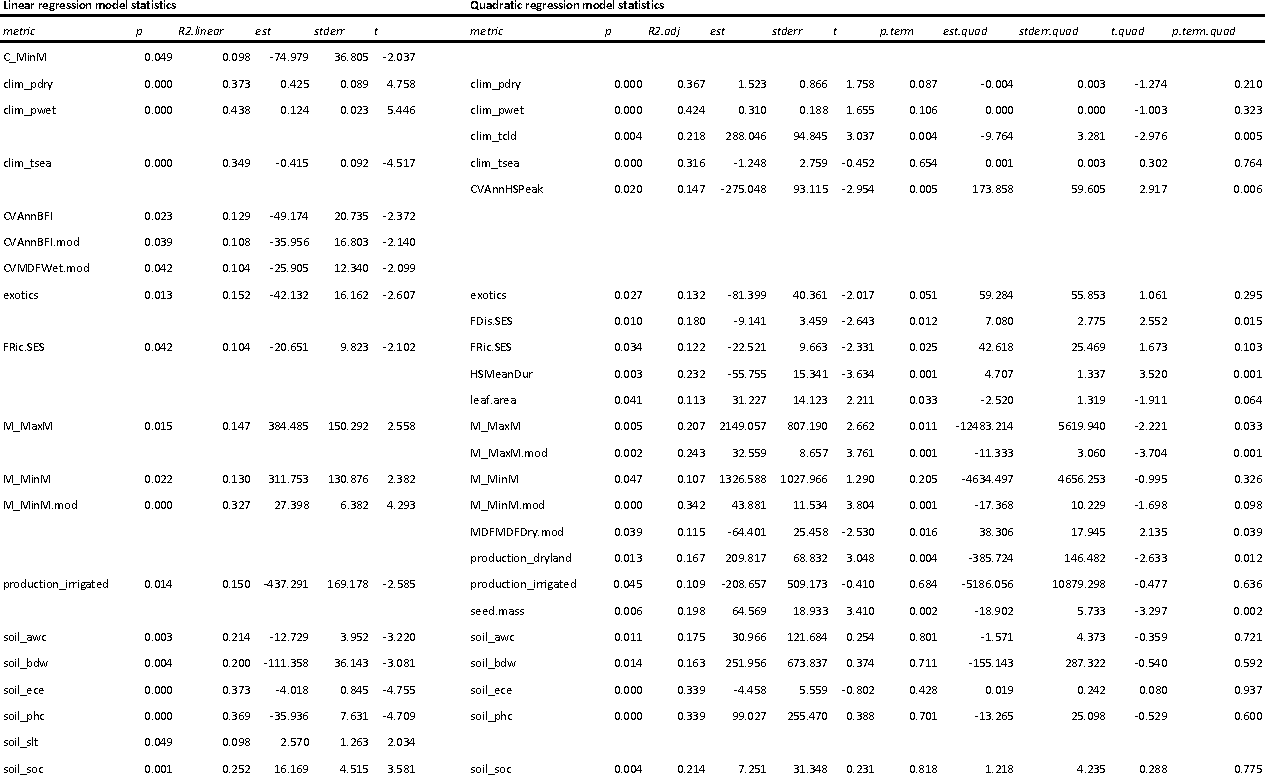
\includegraphics[width=20cm]{regression_stats_sprichChao1.pdf} % figures can be in pdf, png, jpeg or eps format
\caption[Univariate OLS regression statistics for species richness.]{\small{Univariate OLS regression statistics for species richness.}} %The caption in the square bracket is used for the table of figures. The caption in the curved brackets is the one that is printed as actual caption. 
\label{fig:Ch4sup2_F1} % label for cross-referencing
\end{center}
\end{figure}   
\end{landscape}
\clearpage

\begin{landscape}
\begin{figure}[h!]
\begin{center}
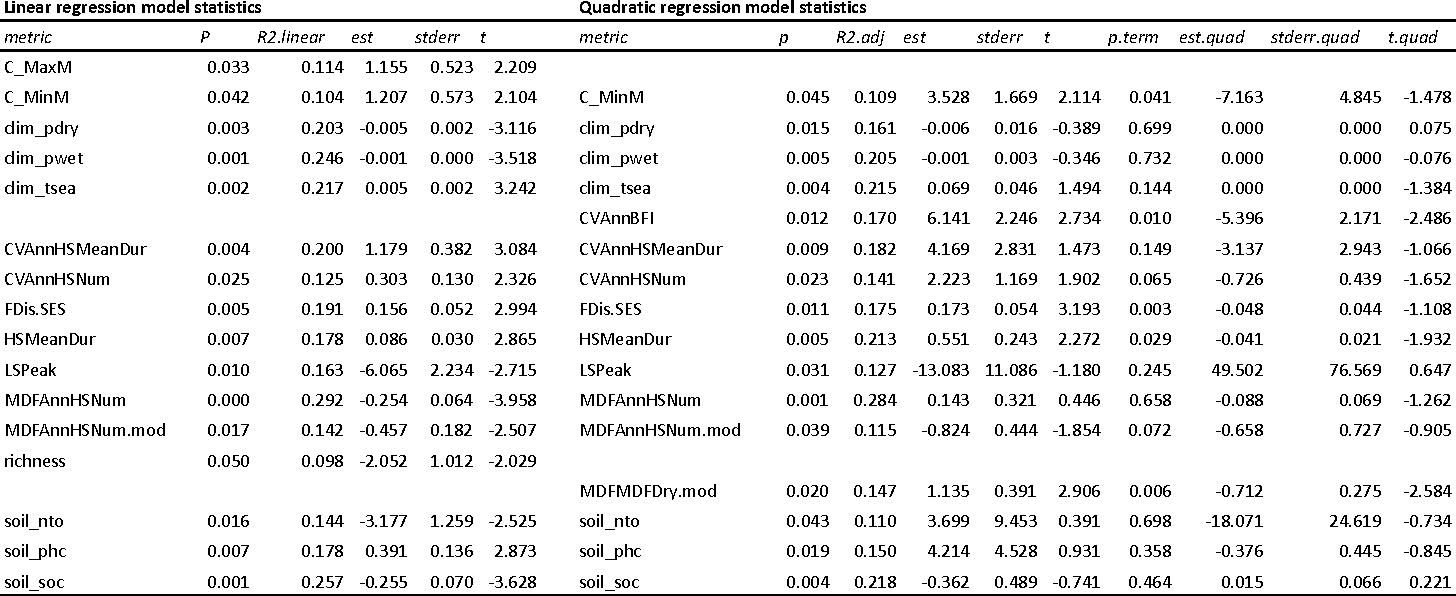
\includegraphics[width=20cm]{S2b.pdf} % figures can be in pdf, png, jpeg or eps format
\caption[Univariate OLS regression statistics for FRic.SES.]{\small{Univariate OLS regression statistics for FRic.SES.}} %The caption in the square bracket is used for the table of figures. The caption in the curved brackets is the one that is printed as actual caption. 
\label{fig:Ch4sup2_F1} % label for cross-referencing
\end{center}
\end{figure}   
\end{landscape}
\clearpage

\begin{landscape}
\begin{figure}[h!]
\begin{center}
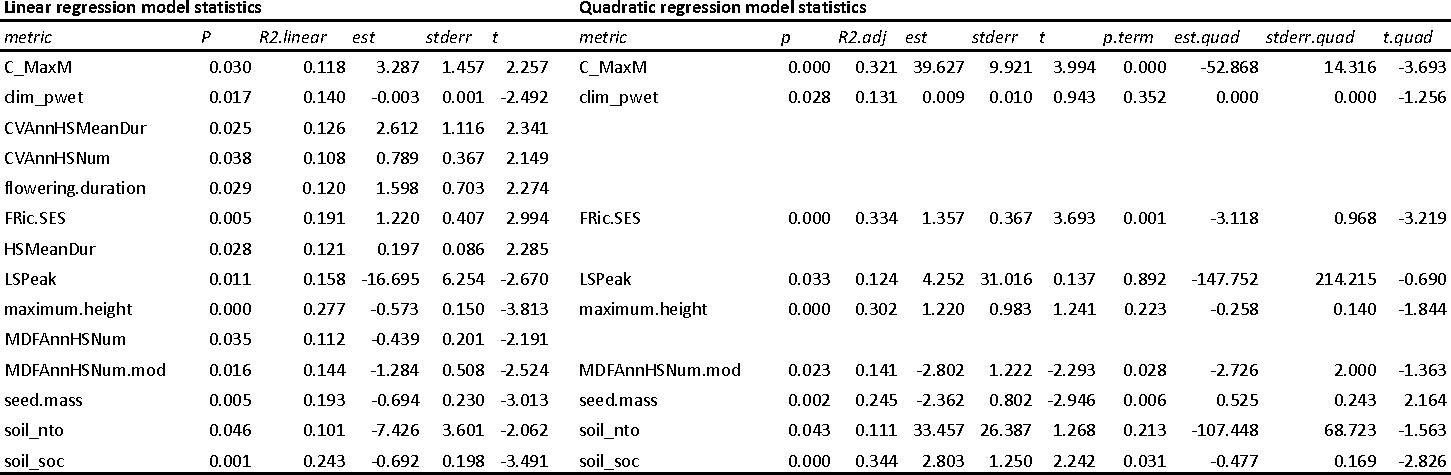
\includegraphics[width=20cm]{S2c.pdf} % figures can be in pdf, png, jpeg or eps format
\caption[Univariate OLS regression statistics for FDis.SES.]{\small{Univariate OLS regression statistics for FDis.SES.}} %The caption in the square bracket is used for the table of figures. The caption in the curved brackets is the one that is printed as actual caption. 
\label{fig:Ch4sup2_F1} % label for cross-referencing
\end{center}
\end{figure}   
\end{landscape}
\clearpage

\begin{landscape}
\begin{figure}[h!]
\begin{center}
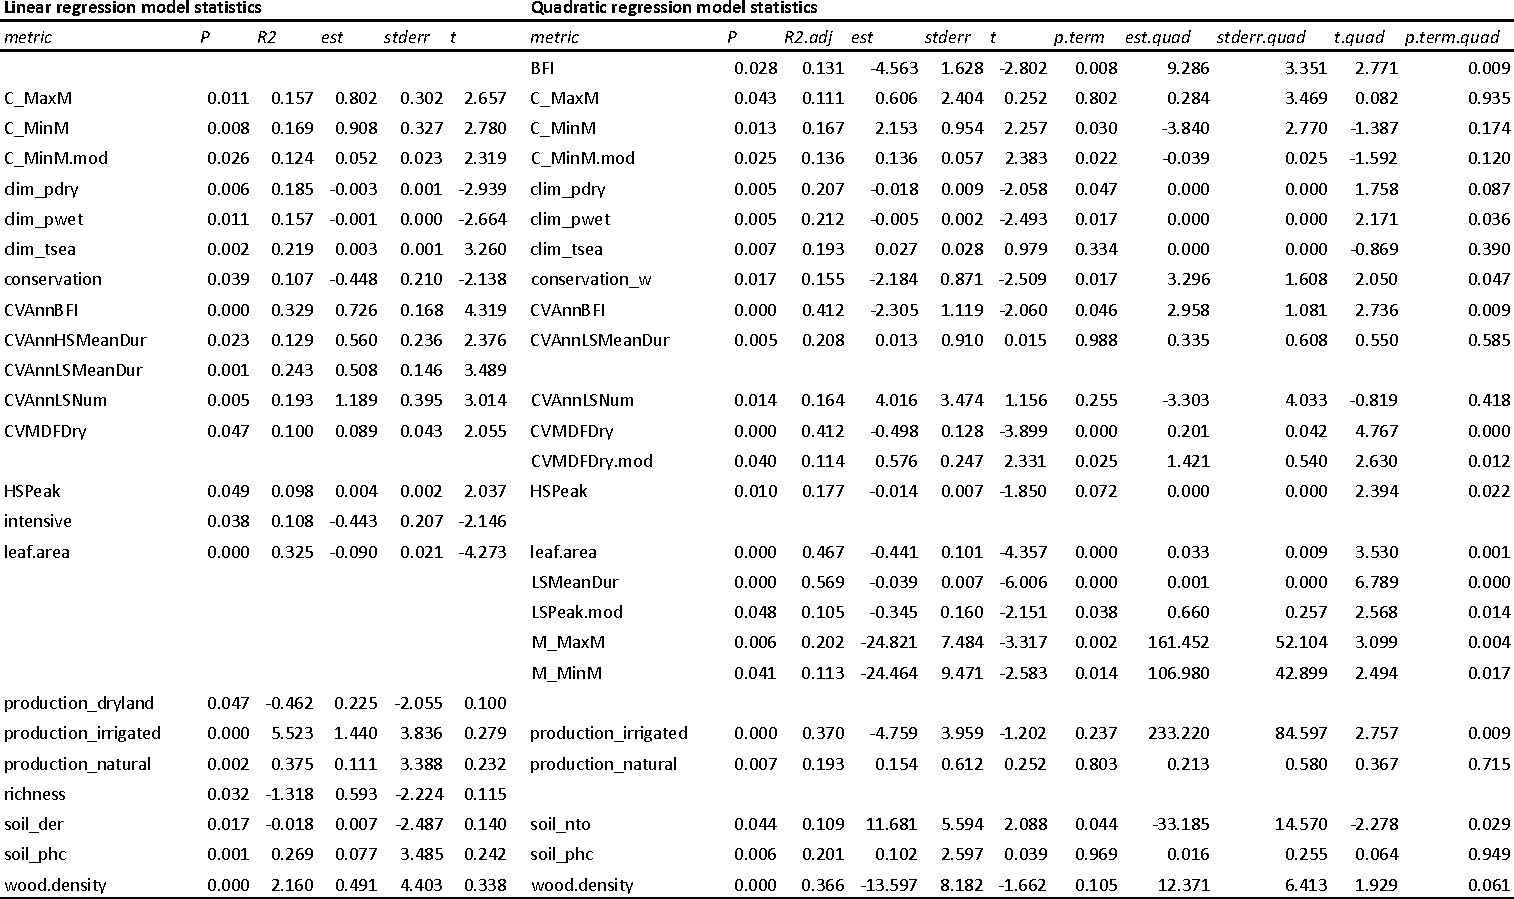
\includegraphics[width=20cm]{S2d.pdf} % figures can be in pdf, png, jpeg or eps format
\caption[Univariate OLS regression statistics for exotic abundance.]{\small{Univariate OLS regression statistics for exotic abundance.}} %The caption in the square bracket is used for the table of figures. The caption in the curved brackets is the one that is printed as actual caption. 
\label{fig:Ch4sup2_F1} % label for cross-referencing
\end{center}
\end{figure}   
\end{landscape}
\clearpage


\clearpage

\chapter[Appendix 4c (Bibliography of trait data sources, supp. Ch4)]{Appendix 4c (Bibliography of trait data sources, supp. Ch4)}
\includepdf[pages=-]{Ch4Bibliography_.pdf}
\clearpage

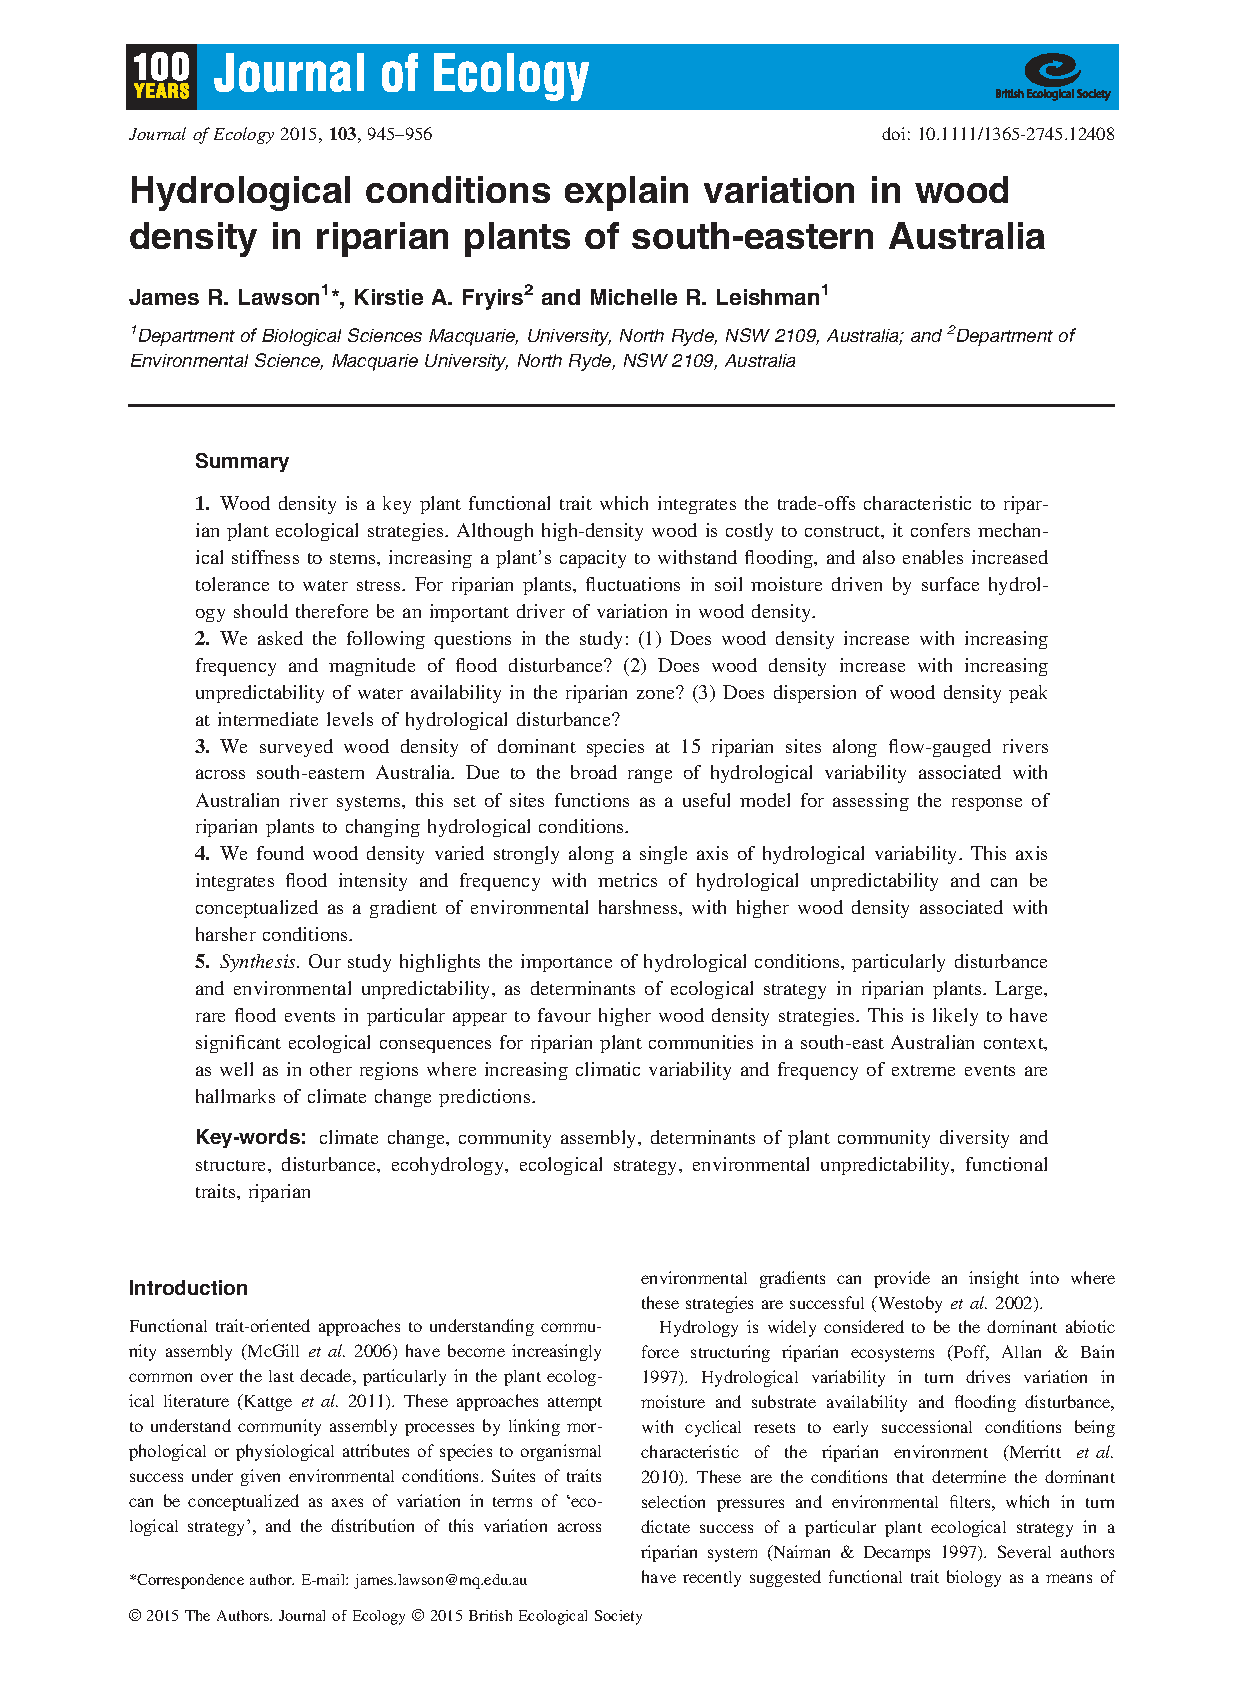
\includepdf[pages=-]{lawson2015a.pdf}
\clearpage

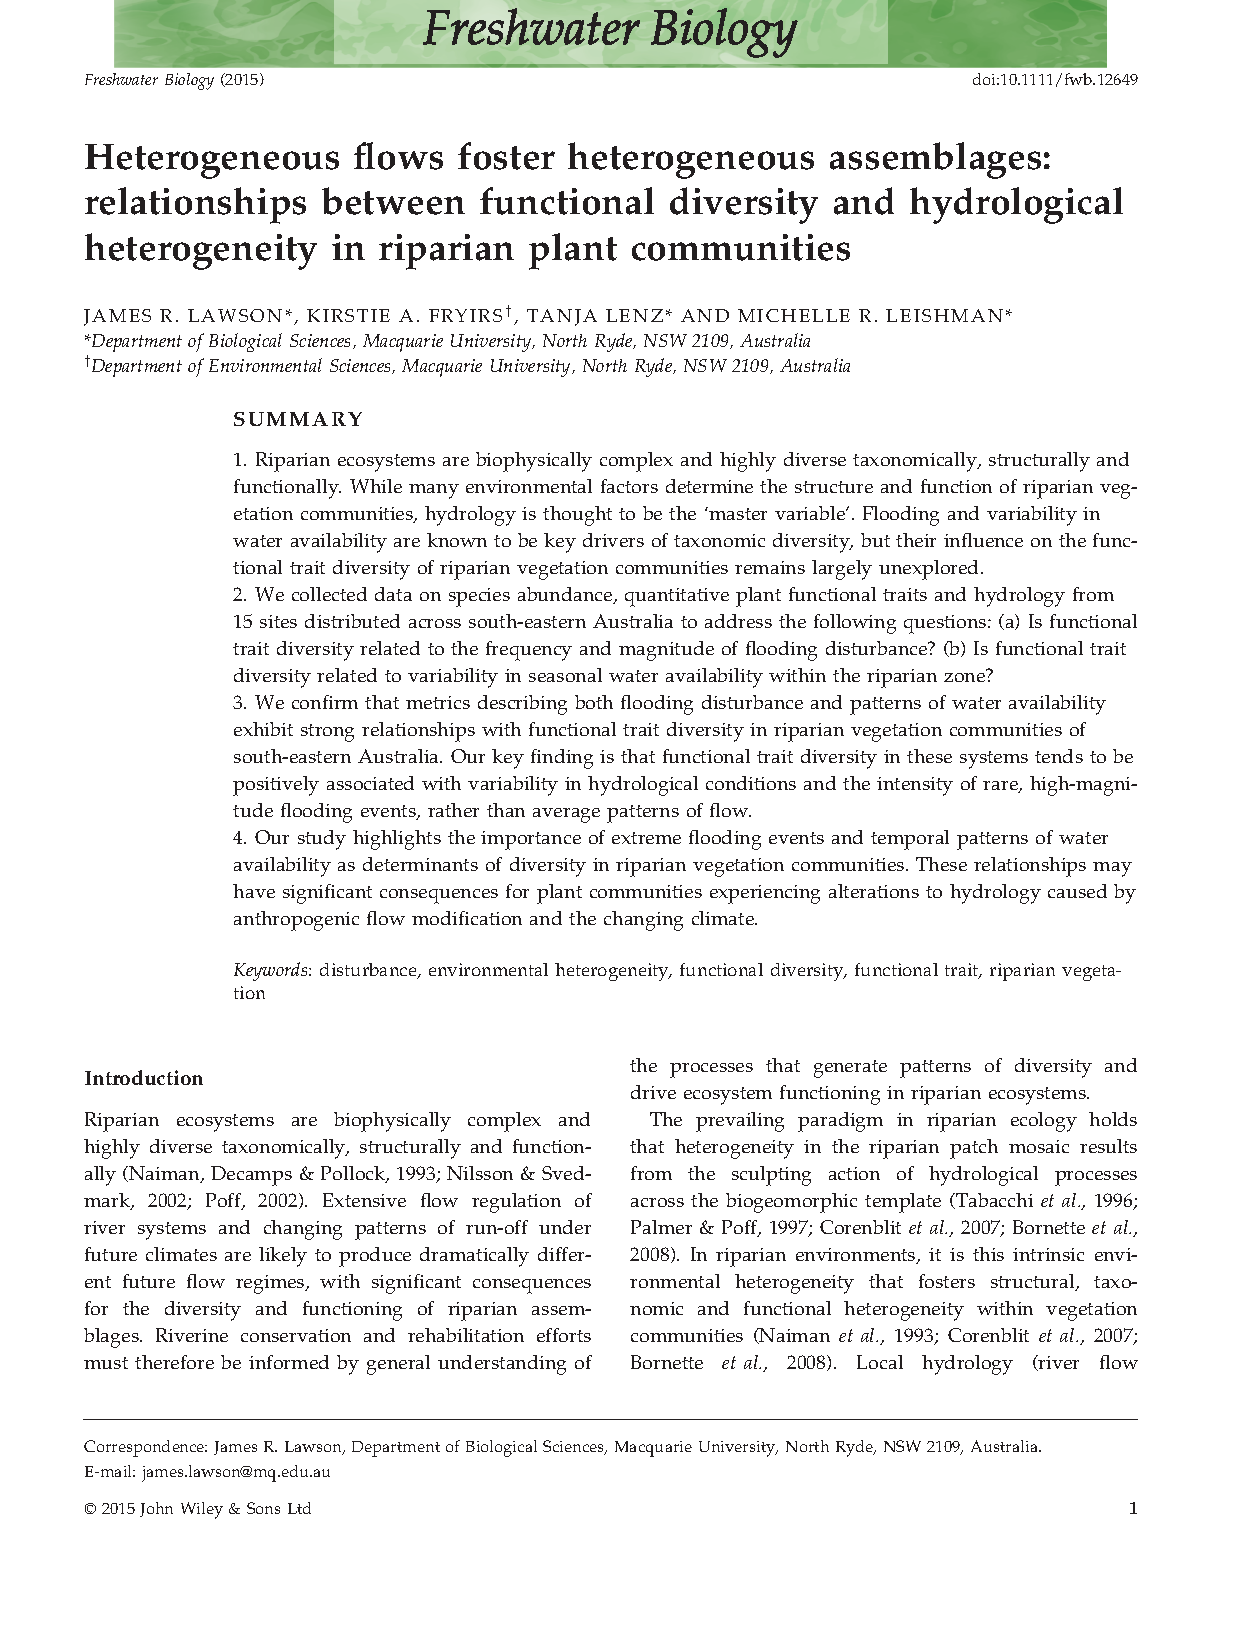
\includepdf[pages=-]{lawson2015b.pdf}
\clearpage

%%%%%%%%%%%%%%%%%%%%%%%%%%%%%%%%%%%%%%%%%%%%%%%%%%%%%%%%%%%%%%%%%%%
\end{document}
%%%%%%%%%%%%%%%%%%%%%%%%%%%%%%%%%%%%%%%%%%%%%%%%%%%%%%%%%%%%%%%%%%%

